\documentclass{ctexart}
% Language setting
% Replace `english' with e.g. `spanish' to change the document language
\usepackage[english]{babel}


\usepackage{amsfonts}
% Set page size and margins
% Replace `letterpaper' with `a4paper' for UK/EU standard size
\usepackage[letterpaper,top=2cm,bottom=2cm,left=3cm,right=3cm,marginparwidth=1.75cm]{geometry}
\usepackage{listings}
\usepackage{xcolor} % 用于颜色支持

\lstset{
    basicstyle=\ttfamily\small,
    keywordstyle=\color{blue},
    commentstyle=\color{green},
    numbers=left, % 显示行号
    frame=single, % 边框
    breaklines=true, % 自动换行
}
% Useful packages


% 自定义颜色
\definecolor{verilog-keyword}{RGB}{0, 0, 255}    % 关键字(蓝色)
\definecolor{verilog-comment}{RGB}{0, 128, 0}    % 注释(绿色)
\definecolor{verilog-string}{RGB}{200, 100, 0}   % 字符串/数字(橙色)
\definecolor{verilog-directive}{RGB}{128, 0, 128} % 预处理指令(紫色)
\definecolor{verilog-background}{RGB}{245, 245, 245} % 背景色(浅灰)

\usepackage{fancyhdr} % 页眉页脚控制
\usepackage{lastpage} % 获取总页数(可选)

% 设置页眉页脚样式
\pagestyle{fancy}
\fancyhf{} % 清除默认页眉页脚

% --- 页眉设置 ---
\fancyhead[L]{\color{brown!50!black!}{\leftmark}}       % 左侧:当前章节标题
\fancyhead[R]{\color{brown!50!black!}{\thepage}}        % 右侧:当前页码

% --- 页脚设置 ---
\fancyfoot[C]{\small \color{brown!50!black!}{高等数学(II) by 404NOTFOUND}} % 居中:自定义文本

\usepackage{amsmath}
\usepackage{tcolorbox}
\usepackage{graphicx}
\usepackage[colorlinks=true, allcolors=blue]{hyperref}
\usepackage{esint}
\usepackage{bm}
\usepackage{float}

% 设置目录链接颜色为黑色
\hypersetup{
    colorlinks=true, % 启用链接颜色
    linkcolor=black, % 目录链接颜色
    anchorcolor=black, % 锚点颜色
    urlcolor=black, % URL 颜色
    citecolor=black % 引用颜色
}
\usepackage{pagecolor} % 用于设置页面背景色

% 定义淡米黄色
\definecolor{pagecream}{RGB}{255, 255, 251}

% 设置页面背景色(取消注释生效)
\pagecolor{pagecream} % 使用定义的米黄色
%\pagecolor{pageivory} % 或切换为其他颜色



\usepackage{xcolor}  % 加载颜色支持
\usepackage{titlesec} % 加载标题格式控制宏包

% 仅修改 section 标题颜色为棕色
\titleformat{\section}
  {\normalfont\Large\bfseries\color{brown!70!black}\centering} % 仅添加颜色
  {\thesection}
  {1em}
  {}

% 仅修改 subsection 标题颜色为棕色
\titleformat{\subsection}
  {\normalfont\large\bfseries\color{brown!70!black}\centering} % 仅添加颜色
  {\thesubsection}
  {1em}
  {}

% 仅修改 subsubsection 标题颜色为棕色
\titleformat{\subsubsection}
  {\normalfont\normalsize\bfseries\color{brown!70!black}\centering} % 仅添加颜色
  {\thesubsubsection}
  {1em}
  {}
 \tcbuselibrary{skins}
\newtcolorbox{myimagebox}[1][]{
    blanker,
    enhanced,
    shadow={1mm}{-0.5mm}{0mm}{black!50!brown},
    width=\textwidth, % 默认宽度(会被参数覆盖)
    auto outer arc,
    size=minimal,
    before upper={\parindent0pt},
    #1 % 允许传入width=0.6\textwidth等参数
}
\tcbuselibrary{breakable}
\let\oldtextbf\textbf
\renewcommand{\textbf}[1]{\textcolor{brown!50!red}{\oldtextbf{#1}}}

\definecolor{bac1}{rgb}{1,0.97,0.93}  % bac1(橙3% + 白97%)
\definecolor{bac2}{rgb}{1,0.97,0.97}  % bac2(红3% + 白97%)

% 定义框架色(中等饱和度)
\definecolor{fra1}{rgb}{1,0.79,0.70}  % fra1(橙30% + 白70%)
\definecolor{fra2}{rgb}{1,0.70,0.70}  % fra2(红30% + 白70%)

% 定义文本色(高饱和度)
\definecolor{tex1}{rgb}{0.40,0.20,0.00}  % tex1(棕60% + 黑40%)
\definecolor{tex2}{rgb}{0.60,0.00,0.00}  % red!60!black(红60% + 黑40%)

\title{高等数学(II)}
\author{404-NOT-FOUND}
\begin{document}
\maketitle
\tableofcontents
\clearpage
\section{重积分}
\subsection{二重积分}
\subsubsection{二重积分的概念与性质}
二重积分的定义与定积分相似。我们先切割区域$D=\bigcup_{i=1}^{n}D_i $,然后在每一个区域找一个近似点,近似值代替这个区域的值,然后进行\textbf{\color{brown!50!red}求和},最后\textbf{\color{brown!50!red}取极限}。因此我们对二重积分有如下定义:

\begin{tcolorbox}[
    colback=bac2,     % 极浅黄色背景
    colframe=fra2,   % 浅黄色边框
    coltitle=white,             % 标题文字白色
    coltext=tex2,
    title=二重积分的定义,
    fonttitle=\bfseries,        % 标题加粗
arc=3mm,                     % 圆角稍大
breakable
]
设$z=f(x;y)$是定义在平面上的有界闭区域D上的函数。如果对D的任意分割$\{D_1,D_2,...,D_n\}$以及任意选择的$(x_i;y_i)\in D_i(i=1,2...,n)$,当$\lambda\to 0$时,和数:
\begin{align*}
    \sum_{i=1}^n f(x_i;y_i)\delta_i
\end{align*}

总有极限,称该极限是$f(x;y)$在区域上的二重积分,记作:
\begin{align*}
    \iint_D f(x;y)\mathrm{d}x\mathrm{d}y\tag{1-1}
\end{align*}

\end{tcolorbox}
根据二重积分的定义,我们可以得到:$\iint_D 1\mathrm{d}x\mathrm{d}y=S_D$。对于几何含义,我们联想到定积分可以表示面积,自然可以判断出二重积分可以代表体积(令$z=f(x;y)$是几何体的高),也就是说:
\begin{align*}
    \iint_D f(x;y)\mathrm{d}x\mathrm{d}y=V(x;y;z)=V_{up}-V_{down}
\end{align*}


\begin{tcolorbox}[
    colback=bac1,     % 极浅黄色背景
    colframe=fra1,   % 浅黄色边框
    coltitle=white,             % 标题文字白色
    coltext=tex1,
    title=二重积分的性质,
    fonttitle=\bfseries,        % 标题加粗
arc=3mm,                     % 圆角稍大
breakable
]
二重积分满足如下性质:

\textbf{\color{brown!50!red}1:数乘} $\iint_D kf(x;y)\mathrm{d}x\mathrm{d}y=k\iint_D f(x;y)\mathrm{d}x\mathrm{d}y$

\textbf{\color{brown!50!red}2:加法} $\iint_D(f+g)\mathrm{d}x\mathrm{d}y=\iint_D f\mathrm{d}x\mathrm{d}y+\iint_D g\mathrm{d}x\mathrm{d}y$

\textbf{\color{brown!50!red}3:保不等式} $\forall f\geq g,(x;y)\in D$,则:$\iint_D f\mathrm{d}x\mathrm{d}y\geq \iint_D g\mathrm{d}x\mathrm{d}y$

\textbf{\color{brown!50!red}4:分片可加性} $D=D_1\cup D_2$,$D_1^*\cap D_2^*=\varphi$ (两个区域完全隔绝),则:$\iint_D f\mathrm{d}\mathrm{d}y=\iint_{D_1}f\mathrm{d}x\mathrm{d}y+\iint_{D_2}f\mathrm{d}x\mathrm{d}y$

\textbf{\color{brown!50!red}5:积分中值定理}  $f\in C(D)$,则$\exists (x_0,y_0)\in D^*$,使得:$\iint_D \mathrm{d}x\mathrm{d}y=S(D)\times f(x_0;y_0)$
\end{tcolorbox}



\textbf{\color{brown!50!red}例:}如果$f(x;y)\geq 0,(x,y)\in D,f\in C(D),\iint_D f(x;y)\mathrm{d}x\mathrm{d}y\geq 0$,求证:$f(x;y)\equiv 0$。

\textbf{\color{brown!50!red}解:}利用积分中值定理,
\begin{align*}
    &\exists (x_0,y_0)\in D,\text{使得}f(x;y)=\delta>0\\
    &\exists D_1\subseteq D,\text{使得}f(x;y)\geq \frac{\delta}{2}\text{在}(x;y)\in D_1\text{成立}\\
    &\iint_D f(x;y)\mathrm{d}x\mathrm{d}y=\iint_{D_1}f(x;y)\mathrm{d}x\mathrm{d}y+\iint_{D_2}f(x;y)\mathrm{d}x\mathrm{d}y\geq \frac{\delta}{2}\times S_{D_1}>0,\text{矛盾}
\end{align*}

\subsubsection{二重积分在直角坐标系的计算}

二重积分的计算本质就是转化成累次积分,即就是:
\begin{tcolorbox}[
    colback=bac2,     % 极浅黄色背景
    colframe=fra2,   % 浅黄色边框
    coltitle=white,             % 标题文字白色
    coltext=tex2,
    title=二重积分的计算方式,
    fonttitle=\bfseries,        % 标题加粗
    arc=3mm                     % 圆角稍大
]
\begin{align*}
    \iint_D f(x;y)\mathrm{d}x\mathrm{d}y=\int_a^b(\int_c^d f(x;y)\mathrm{d}x)\mathrm{d}y\tag{1-2}
\end{align*}
\end{tcolorbox}


我们看第一种情况:$D=\{(x;y),x\in[a,b],\varphi_1(x)\leq y\leq \varphi_2(x)\}$。

\begin{figure}[H]    
\centering     
\renewcommand{\figurename}{图}     
\renewcommand{\thefigure}{1.1}    
\begin{myimagebox}[width=0.36\textwidth] % 直接传入图片尺寸参数      
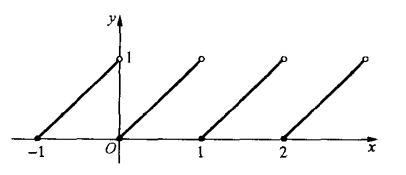
\includegraphics[width=\textwidth]{1.1.png} % 无需重复指定宽度  
\end{myimagebox}     
\caption{\label{fig:1.1}二重积分第一种形式}   
\end{figure}

根据式子1-2,则有
\begin{align*}
    \iint_D f(x;y)\mathrm{d}x\mathrm{d}y&=\int_a^b\left
 ( \int_{\varphi_1(x)}^{\varphi_2(x)} f(x;y)\mathrm{d}y  \right) \mathrm{d}x
\\&=\int_a^b A(x)\mathrm{d}x \tag{1-3}
\end{align*}

如果直观理解,我们相当于是从y轴正方向压扁,每一个自变量的赋值就是这个压扁的所有值的和。

第二种情况类似,$D=\{(x;y),y\in[a,b],\varphi_1(y)\leq x\leq \varphi_2(y)\}$。则:
\begin{align*}
    \iint_D f(x;y)\mathrm{d}x\mathrm{d}y&=\int_a^b\left
 ( \int_{\varphi_1(y)}^{\varphi_2(y)} f(x;y)\mathrm{d}x  \right) \mathrm{d}y
\\&=\int_a^b B(y)\mathrm{d}y \tag{1-4}
\end{align*}

如果是一般情况,我们也可对区域做出切割使其回到前两种情况。累次积分的内层是一个\textbf{\color{brown!50!red}函数},并且\textbf{\color{brown!50!red}上下限是外层变量的函数}。外层则是一个\textbf{\color{brown!50!red}一般定积分}。积分的次序取决于区域和函数的性质。

\textbf{\color{brown!50!red}例}:计算$\iint_D\frac{y}{(1+x^2+y^2)^{3/2}}\mathrm{d}x\mathrm{d}y,D=[0,1]\times[0,1]$

\textbf{\color{brown!50!red}解}:理论上来说谁先谁后都无所谓,但是我们要考虑原函数的简洁性,因此我们考虑先对$y$积分,再对$x$积分。即就是:
    \begin{align*}
    \iint_D\frac{y}{(1+x^2+y^2)^{3/2}}\mathrm{d}x\mathrm{d}y&=
\int_0^1\mathrm{d}x\int_0^1 \frac{y}{(1+x^2+y^2)^{3/2}}\mathrm{d}y\\
&=\int_0^1 \mathrm{d}x \left.[ -\frac{1}{(1+x^2+y^2)^{1/2}} ]\right| _0^1 \\
&=\int_0^1\left [ \frac{1}{(1+x^2)^{1/2}}-\frac{1}{(2+x^2)^{1/2}}\mathrm{d}x    \right ] \\
&=\left.\ln\frac{x+\sqrt{1+x^2}}{x+\sqrt[]{2+x^2} } \right| _0^1\\
&=\ln \frac{2+\sqrt[]{2} }{1+\sqrt[]{3} }
\end{align*}

然而,有的时候\textbf{积分顺序选择不合理,会导致我们有的时候求不出来原函数},我们看下面的这道例题:

\textbf{\color{brown!50!red}例}:计算$\iint_D e^{-y^2}\mathrm{d}x\mathrm{d}y,x\in[0,1],y\in[x,1]$

\textbf{\color{brown!50!red}解}:如果我们先对y积分,我们发现这个原函数不是初等函数。因此我们的想法就是先对x积分,那么区域就可以改写成:$y\in[0,1],x\in[0,y]$,则有:

\begin{align*}
    \iint_D e^{-y^2}\mathrm{d}x\mathrm{d}y&=\int_0^1\mathrm{d}y\int_0^y e^{-y^2}\mathrm{d}x\\
&=\left.\int_0^1\mathrm{d }y[xe^{-y^2}]\right|_0^y\\
&=\int_0^1 ye^{-y^2}\mathrm{d}y\\&=\frac{1}{2}-\frac{1}{2e}  
\end{align*}
\begin{tcolorbox}[
    colback=bac1,     % 极浅橙色背景(几乎白色,但带暖调)
    colframe=fra1,   % 浅橙色边框(柔和)
    coltitle=white!80,    
    coltext=tex1,% 标题文字白色
    title=另一种办法,
    fonttitle=\bfseries,        % 标题加粗
    arc=2mm                     % 轻微圆角
]
当然如果我们强硬地先对$y$积分,利用变积分上限的性质,则可以写作:
\begin{align*}
    \iint_D e^{-y^2}\mathrm{d}x\mathrm{d}y&=\int_0^1\mathrm{d}x\int_x^1 e^{-y^2}\mathrm{d}y\\
&=\int_0^1 A(x)\mathrm{d}x \\
&=\left.xA(x)\right|_0^1-\int_0^1 xA(x)'\mathrm{d}x\\
&=0+\int_0^1xe^{-x^2}\mathrm{d}x= \frac{1}{2}-\frac{1}{2e}  
\end{align*}
\end{tcolorbox}


同理,在参数方程的情况中中也可以这样运算(\textbf{\color{brown!50!red}因为都是对$x,y$积分})。

\textbf{\color{brown!50!red}例}:D为圆摆线:$x(t)=a(t-\sin t),y(t)=a(1-\cos t),t\in[0,2\pi]$与$x$轴围成的区域,计算:$\iint_D y\mathrm{d}x\mathrm{d}y$。

\textbf{\color{brown!50!red}解}:我们考虑先对$y$积分,再对$x$积分。$y$的下限是0,但是上限是关于$x$的函数,且我们难以直接表示。不妨设做$\varphi(x)$。最后一步我们进行换元改变上下限,则有:
\begin{align*}
    \iint_D y\mathrm{d}x\mathrm{d}y&=\int_0^{2\pi a}\mathrm{d}x\int_0^{\varphi(x)} y\mathrm{d}y\\
&=\int_0^{2\pi a}\frac{1}{2}\varphi(x)^2\mathrm{d}x\\   
&=\int_0^{2\pi} \frac{1}{2}[a(1-\cos t)]^2 a(1-\cos t)\mathrm{d}t\\
&=\frac{5\pi a^3}{2}   
\end{align*}

\textbf{\color{brown!50!red}本质上可以在第一步直接换元,就变成了一元定积分。}

我们还要注意,二重积分利用\textbf{\color{brown!50!red}对称性}也可以进行化简计算。例如:如果$f(x;y)$是关于y的\textbf{\color{brown!50!red}奇函数},则在关于y对称的区域上积分为0。如果是关于x的\textbf{\color{brown!50!red}偶函数},则在关于x对称的区域左右两侧积分相等。\textbf{\color{brown!50!red}我们可以利用区间的对称性和被积函数的奇偶性来化简积分运算。}

\begin{figure}[H]    
\centering     
\renewcommand{\figurename}{图}     
\renewcommand{\thefigure}{1.2}    
\begin{myimagebox}[width=0.34\textwidth] % 直接传入图片尺寸参数      
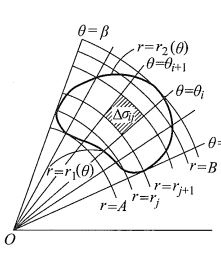
\includegraphics[width=\textwidth]{1.2.png} % 无需重复指定宽度  
\end{myimagebox}     
\caption{\label{fig:1.2}二重积分极坐标形式}   
\end{figure}

对于二重积分的定义方式仍然一样,如同图1.2所示,得出的结果也等同于1-1式。然而,这里的面积是有变化的,它不再是一个小矩形,而是一个小扇形环。因此面积则是:
\begin{align*}
    \delta_i&=\frac{1}{2}(r_i+\Delta r_i)^2\Delta\theta_i-\frac{1}{2}r_i^2\Delta\theta_i\\
    &=r_i\Delta r_i\Delta \theta_i\tag{1-5}
\end{align*}

因此我们的积分形式就变为:
\begin{tcolorbox}[
    colback=bac2,     % 极浅黄色背景
    colframe=fra2,   % 浅黄色边框
    coltitle=white,             % 标题文字白色
    coltext=tex1,
    title=二重积分极坐标计算方式,
    fonttitle=\bfseries,        % 标题加粗
    arc=3mm,                    % 圆角稍大
    breakable,
]
\begin{align*}
    \iint_D f(x;y)\mathrm{d}x\mathrm{d}y=\iint_{D'}f(r\cos\theta;r\sin\theta)r\mathrm{d}r\mathrm{d}\theta\tag{1-6}
\end{align*}
\end{tcolorbox}

这里的$D'$是区域$D$在$r;\theta$平面上的映射。极坐标有很多的应用。例如对一个半径是$R_1--R_2$的圆环,在极坐标下的积分可写成:

\begin{align*}
    \iint_D f(r;\theta)\mathrm{d}r\mathrm{d}\theta=\int_0^{2\pi}\mathrm{d}\theta\int_{R_1}^{R_2}rf(r;\theta)r\mathrm{d}r
\end{align*}

\textbf{\color{brown!50!red}例}:计算$z=1-(x^2+y^2),x^2+y^2\leq 1$与平面$Oxy$围成的几何体的体积。

\textbf{\color{brown!50!red}解}:根据之前二重积分的几何意义,我们只需计算$I=\iint_D 1-x^2-y^2 \mathrm{d}x\mathrm{d}y$即可。我们发现$z$是关于$x,y$对称。因此我们可以只看第一象限。

\begin{align*}
    I&=4\int_0^1\mathrm{d}x\int_0^{\sqrt{1-x^2}}1-x^2-y^2\mathrm{d}y \\
&=4\int_0^1\mathrm{d}x\cdot[(1-x^2)\sqrt{1-x^2}-\frac{1}{3} (1-x^2)^{3/2} ]\\
&=\frac{\pi}{2} 
\end{align*}

第二种想法是在极坐标下计算。令$x=r\cos\theta,y-\sin\theta$,则有:
\begin{align*}
    I&=\iint_{D'}(1-r^2)r\mathrm{d}r\mathrm{d}\theta\\
&=\int_0^{2\pi}\int_0^1(r-r^3)\mathrm{d}r=\frac{\pi}{2}  
\end{align*}

关于区域的映射,也是一个重点。我们需要严格记住极径和极角是对于原点确认的。我们看下面的几个区域:

\begin{figure}[H]    
\centering     
\renewcommand{\figurename}{图}     
\renewcommand{\thefigure}{1.3}    
\begin{myimagebox}[width=0.86\textwidth] % 直接传入图片尺寸参数      
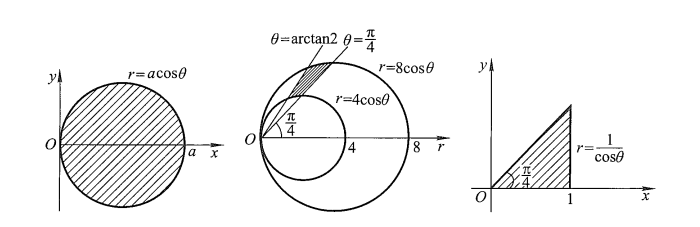
\includegraphics[width=\textwidth]{1.3.png} % 无需重复指定宽度  
\end{myimagebox}     
\caption{\label{fig:1.3}极坐标区域映射}   
\end{figure}

对于左侧,每一个$\theta$对应的极径为$a\cos\theta$。r的取值范围为$[0,r\cos\theta]$。对于第二个,找到一个$\theta$,对应的r的范围为$[4\cos\theta,8\cos\theta]$。第三个图的话,对应的r的范围是$[0,\frac{1}{\cos\theta}]$。

\textbf{\color{brown!50!red}例}:试说明:$I=\int_{-\infty}^{\infty} e^{-x^2}\mathrm{d}x=\sqrt{\pi}$。

\textbf{\color{brown!50!red}解}:我们可以发现,
\begin{align*}
    I^2&=\int_{-\infty}^{\infty} e^{-x^2}\mathrm{d}x\int_{-\infty}^{\infty} e^{-y^2}\mathrm{d}y\\
&=\int_{-\infty}^{\infty}\int_{-\infty}^\infty e^{-x^2-y^2}\mathrm{d}x\mathrm{d}y\\
&=\lim_{a\to\infty}\iint_{x^2+y^2=a^2} e^{-x^2+y^2}\mathrm{d}x\mathrm{d}y\\
&=\lim_{r\to\infty}\int_0^{2\pi}\mathrm{d}\theta\int_0^are^{-r^2}\mathrm{d}r=\pi 
\end{align*}

在选择极坐标积分还是直角坐标积分的选择问题上,一方面要关注积分区域,另一方面也要关注被积函数的特征,例如:

计算$\iint_D \frac{\mathrm{d}x\mathrm{d}y}{(a^2+x^2+y^2)^{3/2}}$,其中$D=\{(x,y)|0\leq x\leq a,0\leq y\leq a\} $

这个区域虽然是矩形,然而如果按照直角坐标积分的话,原函数则太过于困难。由于出现了$x^2+y^2$的形式,我们第一时间可以想到\textbf{\color{brown!50!red}极坐标换元}。而积分函数是关于直线$y=x$对称,因此我们转化成图1.3的第三个图作为积分区域,使用极坐标积分。因此:
\begin{align*}
\iint_D\frac{\mathrm{d}x\mathrm{d}y  }{(a^2+x^2+y^2)^{3/2}}&=2\int_0^{\frac{\pi}{4} }\int_0^
{\frac{r}{\cos\theta} }\frac{a\mathrm{d}r\mathrm{d}\theta }{(a^2+r^2)^{3/2}} \\
&=2\int_0^{\frac{\pi}{4}}\mathrm{d}\theta \left.\times \frac{-1}{(a^2+r^2)^{1/2}} \right|_0^
{\frac{a}{\cos\theta}}\\
 &=\frac{\pi}{2a}-\frac{2}{a}\int_0^\frac{\pi}{4}\frac{\cos\theta\mathrm{d}\theta }
{\sqrt[]{1+\cos\theta^2} }     
\end{align*} 

而后面的积分可以由下面计算:
\begin{align*}
  \int_0^\frac{\pi}{4}\frac{\cos\theta\mathrm{d}\theta }
{\sqrt[]{1+\cos\theta^2} }     &=\int_0^{\frac{\sqrt{2}}{2}}\frac{1}{\sqrt[]{2-t^2} }\mathrm{d}t\\
&=\left.\arcsin{\frac{t}{\sqrt[]{2} }} \right|_0^{\frac{\sqrt[]{2}}{2}  }  \\&=\frac{\pi}{6}  
\end{align*} 

因此可以得到,
\begin{align*}
\iint_D\frac{\mathrm{d}x\mathrm{d}y  }{(a^2+x^2+y^2)^{3/2}}=\frac{\pi}{2a}-\frac{2}{a}\times 
\frac{\pi}{6}=\frac{\pi}{6a}   
\end{align*} 

\subsubsection{二重积分在一般情况下的映射}
极坐标和直角坐标是最简单的两种映射。然而如果映射推广到一般情况,即就是:$x=x(\zeta ,\eta),y=(\zeta,\eta) $,情况又该如何呢?关键是要求出\textbf{\color{brown!50!red}面积微元的比例}。我们在映射后的区域寻找一点$P_0'=(\zeta_0,\eta_0)$,这个点在原来区域内对应的点为$P_0=(x_0,y_0)$。在映射后区域内选择面积微元增量$\mathrm{d}\zeta,\mathrm{d}\eta$,对应的矩形四个顶点为$P_0',P_1',P_2',P_3'$,那么这个矩形的面积为$\Delta \sigma'=\mathrm{d}\zeta\mathrm{d}\eta$。在图1.4表示了这种面积的映射关系。

\begin{figure}[H]    
\centering     
\renewcommand{\figurename}{图}     
\renewcommand{\thefigure}{1.4}    
\begin{myimagebox}[width=0.88\textwidth] % 直接传入图片尺寸参数      
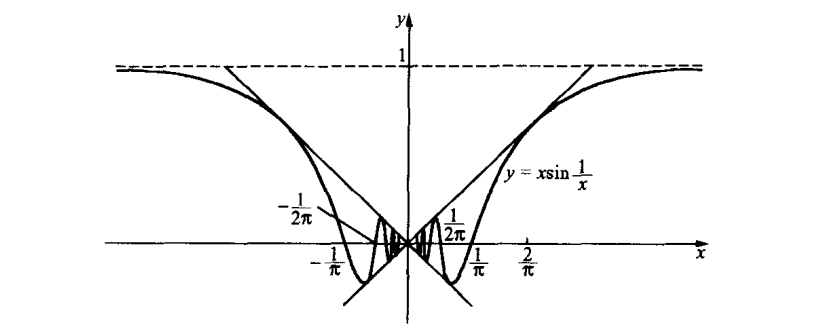
\includegraphics[width=\textwidth]{1.4.png} % 无需重复指定宽度  
\end{myimagebox}     
\caption{\label{fig:1.4}一般坐标映射}   
\end{figure}

我们继续来看,在原来的坐标中,四个顶点为$P_0,P_1,P_2,P_3$,这个图形是一个曲边的四边形,当增量足够小,近似可以看成一个平行四边形,因此这个平行四边形的面积满足:
\begin{align*}
   \Delta \sigma=|\bm{P_0P_1}\times\bm{P_0P_3} |\tag{1-7} 
\end{align*}

接下来我们先计算$x_1-x_0$,即就是:
\begin{align*}
x_1-x_0=\frac{\partial x}{\partial\zeta} \mathrm{d}\zeta 
\end{align*}

这是因为对于$x_1$,增量是由于变量$\zeta$的变化导致函数$x(\zeta,\eta)$的变化。因此类比得到:
\begin{align*}
\bm{P_0P_1}&=(\frac{\partial x}{\partial \zeta}, 
\frac{\partial y}{\partial \zeta})\mathrm{d}\zeta \\
\bm{P_0P_3}&=(\frac{\partial x}{\partial \eta}, 
\frac{\partial y}{\partial \eta})\mathrm{d}\eta \\
\end{align*}

代入1-7,则得到:
\begin{align*}
\Delta \sigma=\left |  \begin{vmatrix}
 \frac{\partial x}{\partial \zeta} & \frac{\partial y}{\partial \zeta}\\
 \frac{\partial x}{\partial \eta} &\frac{\partial y}{\partial \eta}
\end{vmatrix} \Delta \sigma' \right |
\end{align*}

因此,我们就可以得到:
\begin{tcolorbox}[
    colback=bac2,     % 极浅黄色背景
    colframe=fra2,   % 浅黄色边框
    coltitle=white,             % 标题文字白色
    coltext=tex1,
    title=二重积分的一般映射
    fonttitle=\bfseries,        % 标题加粗
    arc=3mm                     % 圆角稍大
]
\begin{align*}
\iint_D f(x;y)\mathrm{d}x\mathrm{d}y=\iint_{D'}f(x(\zeta,\eta);y(\zeta,\eta))\mathrm{d}\zeta
\mathrm{d}\eta\times |\frac{D(x;y)}{D(\zeta;\eta)}|  \tag{1-8}   
\end{align*}
\end{tcolorbox}

根据高数上的所学,在1-8成立的要求是1-7成立,也就是说$x,y$要可以对$\zeta,\eta$求偏微分,因此这\textbf{\color{brown!50!red}要求雅可比行列式处处不为0}(实际上,只要不是一大片为0就没问题),在几何上,\textbf{\color{brown!50!red}这个条件意味着原来的矩形经过映射后必须近似是一个平行四边形}。实际上,1-7可以写成:
\begin{align*}
    \Delta \sigma=\Delta \sigma' |J\textbf{\color{brown!50!red}|}
\end{align*}

例:根据一般映射计算:$\iint_D (x+y)^2e^{x^2-y^2}\mathrm{d}x\mathrm{d}y$,其中$D=\{(x,y)|0\leq x+y\leq 1,0\leq x-y \leq 1\}$

解:不妨令$u=x+y,v=x-y$,则$x=\frac{u+v}{2},y=\frac{u-v}{2}$,则|J|=0.5。因此:
\begin{align*}
\iint_D (x+y)^2e^{x^2-y^2}\mathrm{d}x\mathrm{d}y=\int_0^1\int_0^1u^2e^{uv}\times \frac{1}{2}
\mathrm{d}u\mathrm{d}v =\frac{1}{4}  
\end{align*}

有一类特殊的极坐标积分叫做\textbf{\color{brown!50!red}广义极坐标积分},即就是$x=ar\cos\theta,y=br\sin\theta$,此时的雅可比行列式的结果为:
\begin{align*}
|J|=\begin{vmatrix}
 a\cos\theta &  b\sin\theta\\
 -ar\sin\theta & br\cos\theta
\end{vmatrix}=abr\tag{1-9}
\end{align*}

广义极坐标积分通常在积分区间为椭圆的时候使用。利用一般区域积分还有一种常见的区域为:\textbf{\color{brown!50!red}两类相同函数(四条函数)交出的区域}。如由$y=ax^2,y=bx^2,y=cx,y=dx$围成的区域。这种情况下令$\zeta=\frac{y}{x^2},\eta=\frac{y}{x}$即可。
\begin{tcolorbox}[
    colback=bac1,     % 极浅橙色背景(几乎白色,但带暖调)
    colframe=fra1,   % 浅橙色边框(柔和)
    coltitle=white!80,    
    coltext=tex1,% 标题文字白色
    title=补充知识:利用二重积分证明不等式,
    fonttitle=\bfseries,        % 标题加粗
    arc=2mm                     % 轻微圆角
]
接下来我们介绍一个不等式:\textbf{\color{brown!50!red}Schwarz不等式}。
\begin{align*}
\left(\int_a^bf(x)g(x)\mathrm{d}x \right)^2\leq\int_a^bf(x)^2\mathrm{d}x\int_a^bg(x)^2\mathrm{d}x\tag{1-10}
\end{align*}

它的证明过程与二重积分有关。构造$h(x;y)=[f(x)g(y)-f(y)g(x)]^2$。由于$\iint_D h(x;y)\mathrm{d}x\mathrm{d}y\geq 0$,令区域$D=[a,b]\times[a,b]$,则有:
\begin{align*}
\iint_D h(x;y)\mathrm{d}x\mathrm{d}y&=\int_a^b\int_a^b[f(x)^2g(y)^2+f(y)^2g(x)^2]\mathrm{d}x\mathrm{d}y
-2\int_a^b\int_a^b f(x)f(y)g(x)g(y)\mathrm{d}x\mathrm{d}y\\
=\int_a^bf(x)^2\mathrm{d}x &\int_a^bg(y)^2\mathrm{d}y+ 
\int_a^bf(y)^2\mathrm{d}y\int_a^bg(x)^2\mathrm{d}x -2 \int_a^bf(x)g(x)\mathrm{d}x 
\int_a^bf(y)g(y)\mathrm{d}y\\
&=2\left[\int_a^bf(x)^2\mathrm{d}x\int_a^bg(y)^2\mathrm{d}y\right]-2\left(\int_a^b f(x)g(x)\mathrm{d}x 
\right)^2\\
&=2\left[\int_a^bf(x)^2\mathrm{d}x\int_a^bg(x)^2\mathrm{d}x\right]-2\left(\int_a^b f(x)g(x)\mathrm{d}x 
\right)^2\geq 0
\end{align*}

证毕。这里用了二重积分的一些性质。下面一道题也可以利用二重积分的一些思路去解决。
\end{tcolorbox}

\textbf{\color{brown!50!red}证明}:函数$f(x)$在[0,1]上单调递减且连续,$f(x)>0$,证明:$\frac{\int_0^1xf(x)^2\mathrm{d}x }{\int_0^1xf(x)\mathrm{d}x}\leq 
 \frac{\int_0^1f(x)^2\mathrm{d}x }{\int_0^1f(x)\mathrm{d}x}$

 我们去掉分母,即就是证明:
\begin{align*}
&\int_0^1xf(x)^2\mathrm{d}x \int_0^1f(x)\mathrm{d}x\leq 
\int_0^1f(x)^2\mathrm{d}x \int_0^1xf(x)\mathrm{d}x\\
&\int_0^1xf(x)^2\mathrm{d}x \int_0^1f(y)\mathrm{d}y\leq 
\int_0^1f(y)^2\mathrm{d}y \int_0^1xf(x)\mathrm{d}x\\
&I=\int_0^1\int_0^1xf(x)f(y)[f(x)-f(y)]\mathrm{d}x\mathrm{d}y\leq0\tag{a}
\end{align*}

我们把自变量互换,也就是说:
\begin{align*}
I=\int_0^1\int_0^1yf(x)f(y)[f(y)-f(x)]\mathrm{d}x\mathrm{d}y\leq0\tag{b} 
\end{align*}

两式相加,可得:
\begin{align*}
I=&\frac{1}{2}\int_0^1\int_0^1f(x)f(y)[xf(x)-xf(y)+yf(y)-yf(x)]\mathrm{d}x\mathrm{d}y\\
=&\frac{1}{2}\int_0^1\int_0^1f(x)f(y)(x-y)[f(x)-f(y)]\mathrm{d}x\mathrm{d}y\leq0
\end{align*}

证毕。

\subsection{三重积分}
\subsubsection{三重积分在直角坐标系的计算}
三重积分的定义类似于二重积分。这里不再赘述。

三重积分的计算类似于二重积分,也是化作累次积分。第一种办法是内一重外二重(也就是先对$z$积分,然后对$x,y$积分);第二种办法是内二重外一重(也就是先对$x,y$积分,再对$z$积分)。
\begin{tcolorbox}[
    colback=bac2,     % 极浅黄色背景
    colframe=fra2,   % 浅黄色边框
    coltitle=white,             % 标题文字白色
    coltext=tex2,
    title=三重积分的计算,
    fonttitle=\bfseries,        % 标题加粗
arc=3mm,                     % 圆角稍大
breakable
]
\textbf{\color{brown!50!red}情形1}:积分区间$\Omega=\{(x,y,z);(x,y)\in D,z\in[z_1(x,y),z_2(x,y)]\}$,在几何条件上,我们要求\textbf{\color{brown!50!red}积分区间的侧面是一个柱面,上下底面可以是曲面}。类似于一个圆柱。因此则有:
\begin{align*}
\iiint_\Omega f(x,y,z)\mathrm{d}x\mathrm{d}y\mathrm{d}z=\iint_D\mathrm{d}x\mathrm{d}y
\int_{z_1(x;y)}^{z_2(x;y)}\mathrm{d}z\tag{1-11}  
\end{align*}

\begin{figure}[H]    
\centering     
\renewcommand{\figurename}{图}     
\renewcommand{\thefigure}{1.5}    
\begin{myimagebox}[width=0.44\textwidth] % 直接传入图片尺寸参数      
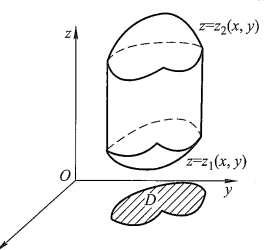
\includegraphics[width=\textwidth]{1.5.png} % 无需重复指定宽度  
\end{myimagebox}     
\caption{\label{fig:1.5}三重积分第一种情况}   
\end{figure}

\textbf{\color{brown!50!red}情形2}:积分区间$\Omega=\{(x,y,z);z\in[a,b]\},(x,y)\in D_z$。\textbf{\color{brown!50!red}在几何上要求上下底面的z是平面。然后在中间去一个Oxy平面,先对取到的平面与积分空间的交面$D_z$积分}。因此:
\begin{figure}[H]    
\centering     
\renewcommand{\figurename}{图}     
\renewcommand{\thefigure}{1.7}    
\begin{myimagebox}[width=0.45\textwidth] % 直接传入图片尺寸参数      
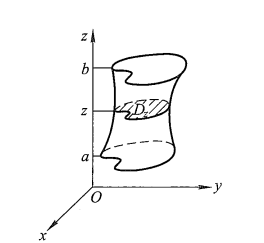
\includegraphics[width=\textwidth]{1.7.png} % 无需重复指定宽度  
\end{myimagebox}     
\caption{\label{fig:1.7}三重积分第二种情况}   
\end{figure}
\begin{align*}
    \iiint_\Omega f(x,y,z)\mathrm{d}x\mathrm{d}y\mathrm{d}z=\int_a^b\mathrm{d}z\iint_{D_z}f(x,y,z)\mathrm{d}x\mathrm{d}y\tag{1-12}
\end{align*}

\textbf{(为了形象记忆,我们可以理解成:情形1压扁积分,情形2抽片积分)}
\end{tcolorbox}

\textbf{\color{brown!50!red}例}:计算 $\iiint_\Omega y\cos(x+z)\mathrm{d}x\mathrm{d}y\mathrm{d}z$,区域由$y=0,z=0,x+z=\frac{\pi}{2},y=\sqrt{x}$围成。

\textbf{\color{brown!50!red}解}:在做三重积分的时候我们习惯于先把积分空间在几何上表达出来。这个几何空间如下图所示:
\begin{figure}[H]    
\centering     
\renewcommand{\figurename}{图}     
\renewcommand{\thefigure}{1.6}    
\begin{myimagebox}[width=0.45\textwidth] % 直接传入图片尺寸参数      
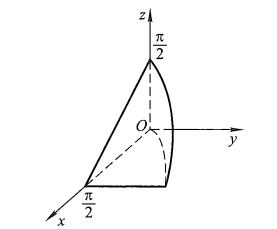
\includegraphics[width=\textwidth]{1.6.png} % 无需重复指定宽度  
\end{myimagebox}     
\caption{\label{fig:1.6}几何空间}   
\end{figure}

\textbf{\color{brown!50!red}我们先要确认$z$的上下界函数。然后再把这个体积“拍扁”到$Oxy$平面上即可。}

\begin{align*}
  \iiint_\Omega y\cos(x+z)\mathrm{d}x\mathrm{d}y\mathrm{d}z&=\iint_D y\mathrm{d}x\mathrm{d}y
\int_0^{\frac{\pi}{2}-x}\cos(x+z)\mathrm{d}z\\  
&=\int_0^\frac{\pi}{2}\mathrm{d}x\int_0^{\sqrt[]{x}}y(1-\sin x)\mathrm{d}y\\
&=\frac{1}{2}\left( \frac{\pi^2}{8}-1  \right) 
\end{align*}

\textbf{\color{brown!50!red}例}:计算$\iint_\Omega e^{-z^2}\mathrm{d}x\mathrm{d}y\mathrm{d}z$,其中$\Omega=\{z\in[0,1],x^2+y^2\leq z^2\}$
\begin{align*}
    \iint_\Omega e^{-z^2}\mathrm{d}x\mathrm{d}y\mathrm{d}z&=\int_0^1e^{-z^2}\mathrm{d}z
\iint_{x^2+y^2\leq z^2}\mathrm{d}x\mathrm{d}y\\
  &=\int_0^1e^{-z^2}\mathrm{d}z\int_0^z r\mathrm{d}r\int_0^{2\pi}\mathrm{d}\theta 
\\&=\pi\int_0^1ze^{-z^2}\mathrm{d} z\\&=\frac{\pi}{2}(1-\frac{1}{e})   
\end{align*}

\subsubsection{三重积分在柱坐标系与球坐标系的计算}
\begin{tcolorbox}[
    colback=bac2,     % 极浅黄色背景
    colframe=fra2,   % 浅黄色边框
    coltitle=white,             % 标题文字白色
    coltext=tex2,
    title=三重积分的柱坐标系计算,
    fonttitle=\bfseries,        % 标题加粗
arc=3mm,                     % 圆角稍大
breakable
]
在柱坐标下,由于$x=r\cos\theta,y=r\sin\theta,z=z$,则在$Oxy$平面下的立方体在$r\theta z$平面下是一个柱体。因此:
\begin{align*}
    \Delta V&=\Delta \sigma z=r\mathrm{d}r\mathrm{d}\theta\\
    \iiint_\Omega f(x;y;z)\mathrm{d}x\mathrm{d}y\mathrm{d}z&=\iiint_{\Omega'}f(r\cos\theta,r\sin\theta,z)\mathrm{d}r\mathrm{d}\theta\mathrm{d}z\tag{1-13}
\end{align*}

这一步用到了式子1-6。
\end{tcolorbox}

\textbf{\color{brown!50!red}例}:利用柱坐标系换元计算$\iiint_\Omega x^2y^2z\mathrm{d}x\mathrm{d}y\mathrm{d}z$,其中$\Omega=\{z\in[0,1],x^2+y^2\leq z^2\}$

\begin{align*}
     \iiint_\Omega x^2y^2z\mathrm{d}x\mathrm{d}y\mathrm{d}z&=\iiint_{\Omega'}zr^4\cos^2\theta\sin
^2\theta  r\mathrm{d}r\mathrm{d}\theta  {d}z \\
&=\int_0^1z\mathrm{d}z \int_0^{2\pi}\cos^2\theta\sin^2\theta\mathrm{d}\theta \int_0^z r^5\mathrm
d{r}\\
&=\int_0^1\frac{z^7}{24}\mathrm{d}z\int_0^{2\pi}\sin^22\theta\mathrm{d}\theta=\frac{\pi}{192}   
\end{align*}

\textbf{\color{brown!50!red}例}:求三重积分,积分空间由柱面$x^2+y^2=1$与平面$z=-1,z=1$围成。
\begin{align*}
    I=\iiint_{\Omega}\frac{\mathrm{d}V }{\sqrt{x^2+y^2+(z-2)^2} } 
\end{align*}

\textbf{\color{brown!50!red}解}:利用柱坐标系换元去计算,则:
\begin{align*}
I&=\int_0^{2\pi}\mathrm{d}\theta \int_{-1}^1\mathrm{d}z\int_0^1\frac{r\mathrm{d}r }{\sqrt{r^2+(z-2)^2}}
\\&=2\pi \int_{-1}^1[(\sqrt{1+(z-2)^2}-|z-2|]\mathrm{d}z\\
&=2\pi \int_{-1}^1\sqrt[]{1+(z-2)^2}\mathrm{d}z  \\
&=\pi[-\sqrt{2}+3\sqrt{10}+\ln (\sqrt{2}-1)-\ln(\sqrt{10}-3)-8    ]  
\end{align*}

\textbf{\color{brown!50!red}注意去根号的时候是要带绝对值的}。

三重积分在球坐标下又是如何计算的呢?球坐标由1.8左图所示。在这里,$\varphi\in[0,\pi],\theta\in[0,2\pi],\rho\in[0,+\infty]$,球坐标换元因此就有:$x=\rho\cos\theta\sin\varphi,y=\rho\sin\theta\sin\varphi,z=\rho\cos\varphi$。
\begin{figure}[H]    
\centering     
\renewcommand{\figurename}{图}     
\renewcommand{\thefigure}{1.8}    
\begin{myimagebox}[width=0.65\textwidth] % 直接传入图片尺寸参数      
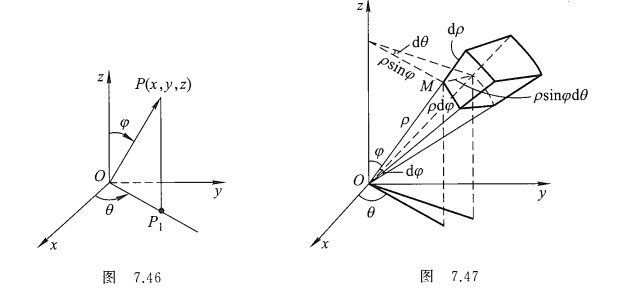
\includegraphics[width=\textwidth]{1.8.png} % 无需重复指定宽度  
\end{myimagebox}     
\caption{\label{fig:1.8}三重坐标的球坐标换元}   
\end{figure}

接下来我们需要计算体积微元比例。如右图所示。右图的体积类似于一个长方体,其体积为:
\begin{align*}
\mathrm{d}V=\rho^2\sin\varphi\mathrm{d}\rho\mathrm{d}\varphi\mathrm{d}\theta   
\end{align*}
\begin{tcolorbox}[
    colback=bac2,     % 极浅黄色背景
    colframe=fra2,   % 浅黄色边框
    coltitle=white,             % 标题文字白色
    coltext=tex2,
    title=三重积分的球坐标计算,
    fonttitle=\bfseries,        % 标题加粗
arc=3mm,                     % 圆角稍大
breakable
]
三重积分的球坐标计算为:
\begin{align*}
    \iiint_{\omega} f(x,y,z)\mathrm{d}V=\iiint_{\Omega'}f(\rho,\theta,\varphi)\rho^2\sin\varphi \mathrm{d}\rho\mathrm{d}\varphi\mathrm{d}\theta\tag{1-14}
\end{align*}
\end{tcolorbox}

\textbf{\color{brown!50!red}例}:计算半径为$r$的球的体积。

\begin{align*}
\iiint_\Omega 1\mathrm{d}V&=\int_0^{2\pi}\mathrm{d}\theta \int_0^\pi\sin\varphi\mathrm{d}\varphi
\int_0^r\rho^2\mathrm{d}\rho\\
&=2\pi \times 2\times \frac{r^3}{3}\\
&=\frac{4\pi r^3}{3}      
\end{align*}

\textbf{\color{brown!50!red}例}:求三重积分:
\[I=\iiint_\Omega \frac{(x+y+z)^2}{(x^2+y^2+z^2)^2}\mathrm{d}V\]

其中积分区间由$x^2+y^2+z^2=4,3z=x^2+y^2,z\geq0$围成。

这种问题首先需要我们画出积分空间。积分空间的示意图如1.9所示。
\begin{figure}[H]    
\centering     
\renewcommand{\figurename}{图}     
\renewcommand{\thefigure}{1.9}    
\begin{myimagebox}[width=0.665\textwidth] % 直接传入图片尺寸参数      
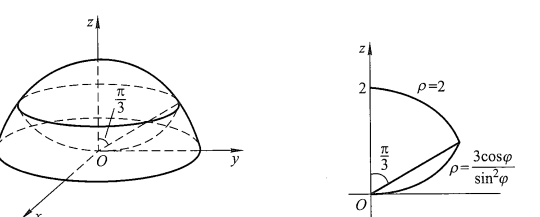
\includegraphics[width=\textwidth]{1.9.png} % 无需重复指定宽度  
\end{myimagebox}     
\caption{\label{fig:1.9}积分空间}   
\end{figure}

因为原函数是很难直接积分的,即使换成球坐标,分子也不好处理。但是我们应该注意到,在这个图形是绕着$z$轴对称的,对于分母部分,$xy,xz,yz$项都会因为对称性被消除,因此其实分子的有效项只有平方项,因此:
\begin{align*}
   I=\iiint_\Omega \frac{(x+y+z)^2}{(x^2+y^2+z^2)^2}\mathrm{d}V=
\iiint_\Omega \frac{x^2+y^2+z^2}{(x^2+y^2+z^2)^2}\mathrm{d}V
=\iiint_\Omega \frac{1}{x^2+y^2+z^2}\mathrm{d}V
\end{align*}

接下来我们要使用球坐标换元。我们先根据积分空间判断,这一一个复合空间(球空间和抛物面空间),交面为$z=1$。在这个面上下,参数的取值范围略有不同。首先我们可以发现,无论是哪个部分,$\theta\in[0,2\pi]$。对于上面的积分$I_1$,我们发现$\rho\in[0,2],\varphi\in[0,\frac{\pi}{3}]$,因此可以计算出:
\begin{align*}   I_1&=\int_0^{2\pi}\mathrm{d}\theta\int_0^2\mathrm{d}r\int_0^{\pi/3} \sin\varphi\mathrm{d}\varphi 
\\&= 2\pi\times2\times \frac{1}{2}=2\pi 
\end{align*}

对于下面的讨论略显的复杂,因为$\rho$的范围是根据$\phi$决定的,此时根据$3z=x^2+y^2$换元得到,$3\cos\varphi=\rho\sin\varphi^2$,即就是$\rho=\frac{3\cos\varphi}{\sin^2\phi}$。因此对这一部分的积分$I_2$可表示为:

\begin{align*} I_2&=\int_0^{2\pi}\mathrm{d}\theta\int_{\pi/3}^{\pi/2} \sin\varphi\mathrm{d}\varphi 
\int_0^{3\cos\varphi/\sin^2\varphi }\mathrm{d}r
\\&= 2\pi\times \int_{\pi/3}^{\pi/2} \frac{3\cos\varphi }{\sin\varphi} \mathrm{d}\varphi
\\&=6\pi\ln\frac{2}{\sqrt{3}} 
\end{align*}

因此原积分可以表示为:
\begin{align*}
    I=I_1+I_2=2\pi\left(1-\ln\frac{\sqrt{3}}{2}\right)
\end{align*}

\subsubsection{三重积分在一般情况下的映射}
这里与二重积分是类似的,我们不加证明地给出定理:
\begin{tcolorbox}[
    colback=bac2,     % 极浅黄色背景
    colframe=fra2,   % 浅黄色边框
    coltitle=white,             % 标题文字白色
    coltext=tex2,
    title=三重积分在一般情况下的映射,
    fonttitle=\bfseries,        % 标题加粗
arc=3mm,                     % 圆角稍大
breakable
]
设从$\Omega'\to\Omega$有一个映射,使得$x=x(u,v,w),y=y(u,v,w),z=z(u,v,w),(u,v,w)\in\Omega'\text{且在}\Omega'$上一阶连续可导。则:
\begin{align*}
   \iiint_\Omega f(x,y,z)\mathrm{d}x\mathrm{d}y\mathrm{d}z=\iiint_{\Omega'}
f(x(u,v,w),y(u,v,w),z(u,v,w)|\bm{J} |\mathrm{d}u\mathrm{d}v\mathrm{d}w\tag{1-15}
\end{align*}

其中:
\begin{align*}
    |\bm{J} |=\frac{D(x,y,z)}{D(u,v,w)}=\begin{Vmatrix}
 \frac{\partial x}{\partial u} & \frac{\partial y}{\partial u} & \frac{\partial z}{\partial u}\\
 \frac{\partial x}{\partial v} &\frac{\partial y}{\partial v}  &\frac{\partial z}{\partial v} \\
 \frac{\partial x}{\partial w} & \frac{\partial y}{\partial w} &\frac{\partial z}{\partial w}
\end{Vmatrix} \tag{1-16}
\end{align*}
\end{tcolorbox}

一种应用是椭球积分。例如下面的例题。

\textbf{例:}求解下面的积分,其中$\Omega: \frac{x^2}{a^2}+\frac{y^2}{b^2}+\frac{z^2}{c^2}\leq 1$。
\begin{align*}
    I=\iiint_\Omega (1-\frac{x^2}{a^2}-\frac{y^2}{b^2}-\frac{z^2}{c^2})^{3/2}\mathrm{d}V
\end{align*}

\textbf{解:}我们做换元,即就是$x=a\rho\cos\theta\sin\varphi,y=b\rho\sin\theta\sin\varphi,z=c\rho\cos\varphi$,计算这个雅可比行列式算得:
\begin{align*}
    |\bm{J} |=abc\rho^2\sin\varphi\tag{1-17}
\end{align*}

因此根据公式得到:
\begin{align*}  
I&=abc\int_0^{2\pi}\mathrm{d}\theta\int_0^\pi\sin\varphi\mathrm{d}
\varphi\int_0^1(1-\rho^2)^{3/2}\rho^2\mathrm{d}\rho\\
&=abc\times2\pi\times 2\times \int_0^{\pi/2}\cos^4\beta\sin^2\beta\mathrm{d} \beta \\
&=4\pi abc\times\frac{\pi}{32}=8\pi^2 abc
\end{align*}

最后两步是使用了Wallis公式。

\subsection{重积分的应用}
\subsubsection{平面面积,空间体积计算}
我们在前两个部分介绍过,$S_D=\iint_D1\mathrm{d}\delta,V_\Omega=\iiint_\Omega 1\mathrm{d}V$。

\textbf{\color{brown!50!red}例}:计算曲面$z=x^2+3y^2$与$z=8-x^2-y^2$围成的体积。

这道题最难的地方是还原出几何空间,如下图所示。
\begin{figure}[H]    
\centering     
\renewcommand{\figurename}{图}     
\renewcommand{\thefigure}{1.10}    
\begin{myimagebox}[width=0.5\textwidth] % 直接传入图片尺寸参数      
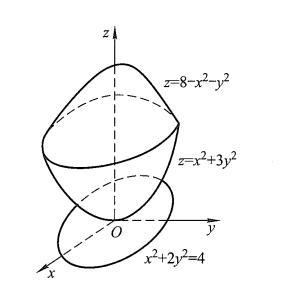
\includegraphics[width=\textwidth]{1.10.png} % 无需重复指定宽度  
\end{myimagebox}     
\caption{\label{fig:1.10}积分空间}   
\end{figure}

在这两个交面上,联立可得:
\begin{align*}
    x^2+3y^2&=8-x^2-y^2\\
    x^2+2y^2&=4
\end{align*}

接下来我们要思考使用哪一种办法去解决,显然在这里使用压扁法更好(使用切片法会发现这个交界面不是平整的)。因此我们可以这样计算:
 \begin{align*}
V & = \iint_D\mathrm{d}x\mathrm{d}y\int_{x^2+3y^2}^{8-x^2-y^2}\mathrm{d}z\\ 
& = \iint_D(8-2x^2-4y^2)\mathrm{d}x\mathrm{d}y
\\&=\int_0^{2\pi}\mathrm{d}\theta\int_0^1(8-8r^2)\cdot2\sqrt{2}r\mathrm{d}r\\
&=8\sqrt{2}\pi  
\end{align*}

最后两步使用了椭圆换元,$x=2r\cos\theta,y=\sqrt{2}r\sin\theta$,计算雅可比行列式可得到$|J|=2\sqrt{2}r$。

\subsubsection{曲面面积计算}
\begin{figure}[H]    
\centering     
\renewcommand{\figurename}{图}     
\renewcommand{\thefigure}{1.11}    
\begin{myimagebox}[width=0.45\textwidth] % 直接传入图片尺寸参数      
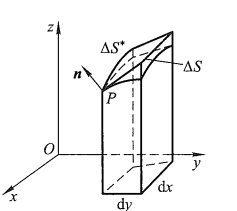
\includegraphics[width=\textwidth]{1.11.png} % 无需重复指定宽度  
\end{myimagebox}     
\caption{\label{fig:1.11}曲面面积的计算}   
\end{figure}

我们假设空间曲面的方程为:$z=f(x,y),f(x,y)\in D,D$是空间曲面在$Oxy$平面上的投影。我们考虑曲面上的任意一点点$P(x,y,z)$,并且考虑两个增量:$\mathrm{d}x,\mathrm{d}y>0$,把$\Delta \sigma=\mathrm{d}x\mathrm{d}y$,小微元曲面面积为$\Delta S$。

过$P$做$S$的切平面,切平面上的微元面积记作$\Delta S^*$,则我们有:
\begin{align*}
    \Delta \sigma=|\cos \bm{r}|\Delta S^*\tag{1-18} 
\end{align*}

其中$\bm{r}$是过P点的法向量$\bm{n}$与$z$正半轴夹角。这一点是好理解的,类比曲线长度和切线长度的关系。

而继续计算可知,法向量可表示为:
\begin{align*}
    \bm{n}=(f_x(x,y),f_y(x,y),-1)\tag{1-19}
\end{align*}

因此带入1-18,可以得到:
\begin{align*}
    \Delta S^*&={\sqrt{f_x(x,y)^2+f_y(x,y)^2+1}}\Delta\sigma\\
 \mathrm{d}S&={\sqrt{f_x(x,y)^2+f_y(x,y)^2+1}}\mathrm{d}\sigma
\end{align*}

\begin{tcolorbox}[
    colback=bac1,     % 极浅黄色背景
    colframe=fra1,   % 浅黄色边框
    coltitle=white,             % 标题文字白色
    coltext=tex1,
    title=Cauchy柯西不等式,
    fonttitle=\bfseries,        % 标题加粗
arc=3mm,                     % 圆角稍大
breakable
]
因此曲面面积的计算公式为:
\begin{align*}
S&=\iint_D{\sqrt{f_x(x,y)^2+f_y(x,y)^2+1}}\mathrm{d}\sigma\tag{1-20} 
\end{align*}
\end{tcolorbox}
其实1-19式的来源也比较简单,类似之前学习证明二重积分一般映射一样,曲面有两条向量可以表示为$(\mathrm{d}x,0,f_x'\mathrm{d}x)$与$(0,\mathrm{d}y,f_y'\mathrm{d}y)$。二者叉乘就可以表示法向量了。

\textbf{\color{brown!50!red}例}:计算圆柱面$x^2+z^2=R^2(R>0)$被圆柱面$x^2+y^2=R^2$所割部分在第一卦限面积。

这个题首先需要\textbf{\color{brown!50!red}求出曲面的方程},即就是:$z=\sqrt{R^2-x^2}$。然后求积分的区域,即就是$x^2+y^2=R^2$。然后求出一些参数,$f_x=\frac{-x}{\sqrt{R^2-x^2}},f_y=0$。因此:
\begin{align*}
    S&=\int_0^R\mathrm{d}x\int_0^{\sqrt{R^2-x^2} }\sqrt{\frac{x^2}{R^2-x^2}+0+1 }\mathrm{d}y
\\&=\int_0^R R\mathrm{d}y=R^2  
\end{align*}

这里注意,积分顺序的选择会大大改变计算量。

对于一般参数化的曲面,面积如何计算?记$x=x(u,v),y=y(u,v),z=z(u,v)$。那么我们可以在曲面上找到两个向量,计算法向量,然后类似于之前的做法即可。
\begin{align*}
 &\bm{a}  =(\frac{\partial x}{\partial  u},\frac{\partial y}{\partial  u},\frac{\partial z}{\partial  u})
\qquad  
\bm{b}  =(\frac{\partial x}{\partial  v},\frac{\partial y}{\partial  v},\frac{\partial z}{\partial  v})
\\
&\bm{n} =\bm{a} \times \bm{b} =(\frac{D(y,z)}{D(u,v)},\frac{D(x,z)}{D(u,v)},\frac{D(x,y)}{D(u,v)})
=(A,B,C)\tag{1-21}
\end{align*}
\begin{tcolorbox}[
    colback=bac1,     % 极浅黄色背景
    colframe=fra1,   % 浅黄色边框
    coltitle=white,             % 标题文字白色
    coltext=tex1,
    title=曲面面积的参数方程法则,
    fonttitle=\bfseries,        % 标题加粗
arc=3mm,                     % 圆角稍大
breakable
]
因此曲面面积可计算为:
\begin{align*}
    S=\iint_{D'}\sqrt{A^2+B^2+C^2}\mathrm{d}u\mathrm{d}v\tag{1-22}
\end{align*}

所以我们只需要求出参数$A,B,C$即可。为了计算方便,我们可以验证:
\begin{align*}
A^2+B^2+C^2=EG-F^2\tag{1-23}\\
E=x_u^2+y_u^2+z_u^2\\
F=x_ux_v+y_uy_v+z_uz_v\\
G=x_v^2+y_v^2+z_v^2
\end{align*}
\end{tcolorbox}

\textbf{例}:已知曲面$S$的参数方程为:
\[
\mathbf{r}(u,v) = (u\cos v, u\sin v, v), \quad 0 \leq u \leq 1, \ 0 \leq v \leq 2\pi
\]
求该曲面的面积。

\textbf{解:}首先计算各项系数:

\begin{align*}
E &= \left(\frac{\partial x}{\partial u}\right)^2 + \left(\frac{\partial y}{\partial u}\right)^2 + \left(\frac{\partial z}{\partial u}\right)^2 \\
  &= (\cos v)^2 + (\sin v)^2 + 0^2 = 1 \\
F &= \frac{\partial x}{\partial u}\frac{\partial x}{\partial v} + \frac{\partial y}{\partial u}\frac{\partial y}{\partial v} + \frac{\partial z}{\partial u}\frac{\partial z}{\partial v} \\
  &= \cos v (-u\sin v) + \sin v (u\cos v) + 0 \cdot 1 = 0 \\
G &= \left(\frac{\partial x}{\partial v}\right)^2 + \left(\frac{\partial y}{\partial v}\right)^2 + \left(\frac{\partial z}{\partial v}\right)^2 \\
  &= (-u\sin v)^2 + (u\cos v)^2 + 1^2 = u^2 + 1
\end{align*}

最终曲面积分为:
\[
S = \int_0^{2\pi} \int_0^1 \sqrt{u^2 + 1}\,du\,dv= \pi \left(\sqrt{2} + \ln(1+\sqrt{2})\right)
\]


\subsection{习题补充与拓展}
\textbf{\color{brown!50!red}例1}:设区域$D$是由$x=R,y=0,y=\frac{2}{R}x-1$围成,计算:
\begin{align*}
     \lim_{R\to\infty} \iint_D e^{-x}\arctan{\frac{y}{x} }\mathrm{d}x\mathrm{d}y 
\end{align*}

\textbf{\color{brown!50!red}解}:这个问题不是直接计算得到的,原函数基本来说很难计算。因此我们需要另辟蹊径。利用\textbf{积分中值定理},存在点$(x_0,y_0)\in D$,使得:
\begin{align*} 
   \iint_D e^{-x}\arctan{\frac{y}{x} }\mathrm{d}x\mathrm{d}y&=e^{-x_0}\arctan{\frac{y_0}{x_0} }
\cdot  S_D\\
&=\frac{R}{4}e^{-x_0}\arctan{\frac{y_0}{x_0} }
\end{align*}

在这里,$\frac{R}{2}\leq x_0\leq R,0\leq y_0\leq 1,R\to\infty$时,有:
\begin{align*} 
  \left| \iint_D e^{-x}\arctan{\frac{y}{x} }\mathrm{d}x\mathrm{d}y
\right|\leq \frac{R}{4}e^{-\frac{R}{2}}\arctan{\frac{2}{R}}\to0
\end{align*}

夹逼定理,原式为0。

\textbf{\color{brown!50!red}例2}:做极坐标变换,将二重积分
\begin{align*} 
\iint_D f(\sqrt{x^2+y^2})\mathrm{d}x\mathrm{d}y
\end{align*}

转化为定积分。其中$D=\{(x,y)| 0\leq y\leq x\leq 1\}$

\textbf{\color{brown!50!red}解}:令$x=r\cos\theta,y=r\sin\theta$,化成定积分就要先对$\theta$积分。这个积分区域是右下三角。因此:
\begin{align*} 
\iint_D f(\sqrt{x^2+y^2})\mathrm{d}x\mathrm{d}y&=\iint_Df(r)r\mathrm{d}r\mathrm{d}\varphi\\
&=\int_0^\frac{\pi}{4} \mathrm{d}\varphi\int_0^\frac{1}{\cos\varphi}f(r)r\mathrm{d}r
\end{align*}

但这还不是定积分的形式。因此这里的\textbf{\color{brown!50!red}积分顺序需要变化},也就是说\textbf{\color{brown!50!red}要先对$\varphi$积分}。当$0\leq r\leq 1$时,$ 0\leq\theta\leq\frac{\pi}{4}$;当$1 \leq r \leq \sqrt{2}$的时候,$\arccos{\frac{1}{r}}\leq\theta\leq\frac{\pi}{4}$,因此:
\begin{align*} 
\iint_Df(r)r\mathrm{d}r\mathrm{d}\varphi
&=\int_0^1 \mathrm{d}r\int_0^\frac{\pi}{4} f(r)r\mathrm{d}\varphi+
\int_1^{\sqrt{2}}\mathrm{d}r\int_{\arccos \frac{1}{r}}^\frac{\pi}{4}f(r)r\mathrm{d}\varphi\\
 &=\frac{\pi}{4}\int_0^1 f(r)r\mathrm{d} r+\int_1^{\sqrt{2}}(\frac{\pi}{4}-\arccos \frac{1}{r})f(r)r\mathrm{d}r\\
&=\frac{\pi}{4}\int_0^{\sqrt{2}}f(r)r\mathrm{d}r-  \int_1^{\sqrt{2}}\arccos{\frac{1}{r}}f(r)r\mathrm{d}r
\end{align*}

\textbf{\color{brown!50!red}例3}:计算
\begin{align*} 
&(1)\qquad\iint_D\left(\sqrt{\frac{x-c}{a}}+\sqrt{\frac{y-c}{b}}\right)\mathrm{d}x\mathrm{d}y\\
&(2)\qquad\iint_\Omega(x+y)\mathrm{d}x\mathrm{d}y
\end{align*}

其中$D$由曲线$\sqrt{\frac{x-c}{a}}+\sqrt{\frac{y-c}{b}}=1,x=c,y=c(a,b,c>0)$围成。$\Omega$ 由曲线 $y^2=2x,x+y=4,x+y=12$围成。

\textbf{\color{brown!50!red}解}:这两道题都涉及到换元。第一题是\textbf{\color{brown!50!red}广义极坐标换元}。令$x=c+a\rho\cos^4\theta,y=c+b\rho\sin^4\theta$。那么换元后的积分区域变为$0\leq\theta\leq\frac{\pi}{2},0\leq\rho\leq1$。对于雅可比行列式,我们可以计算:
\begin{align*} 
|J|=\begin{Vmatrix}
 a\cos^4\theta & b\sin^4\theta \\
 -4a\rho\cos^3\theta\sin\theta & 4b\rho\sin^3\theta\cos\theta
\end{Vmatrix}=4ab\rho\cos^3\theta\sin^3\theta
\end{align*}

因此:
\begin{align*} 
\iint_D\left(\sqrt{\frac{x-c}{a}}+\sqrt{\frac{y-c}{b}}\right)\mathrm{d}x\mathrm{d}y
&=\int_0^{\frac{\pi}{2}}\mathrm{d}\theta\int_0^1  4ab\rho^{\frac{3}{2}}\cos^3\theta\sin^3\theta
\mathrm{d}\rho\\
&=\frac{2ab}{15}  
\end{align*}

对于第二题,如果不换元我们发现无论积分顺序如何都会要分区域去计算,但是如果我们按照$x+y$方向“压扁”计算,则计算难度会小得多。实际上,换元法就是把图象“\textbf{\color{brown!50!red}按照不同的方式去压扁}”,只要二者线性无关即可(这也解释了为什么雅可比行列式不能为0)。因此令$u=x+y,v=y$。对于$y^2-2x\leq 0$这个区域进行化简,新的区域为$4\leq u\leq 12,-1-\sqrt{2u+1}\leq v\leq -1+\sqrt{2u+1}$,雅可比行列式结果为1,因此:
\begin{align*} 
\iint_\Omega(x+y)\mathrm{d}x\mathrm{d}y&=\int_4^{12}u\mathrm{d}u\int_{-1-\sqrt{2u+1}}  
^{-1+\sqrt{2u+1}}\mathrm{d}v\\
&=\int_4^{12} 2u\sqrt{2u+1}\mathrm{d}u\quad (\sqrt{2u+1}=t)\\
&=\frac{8156}{15}    
\end{align*}

\textbf{\color{brown!50!red}例4}:计算
\begin{align*} 
\iiint_\Omega xyz\mathrm{d}x\mathrm{d}y\mathrm{d}z
\end{align*}

其中$\Omega$为$x^2+y^2+z^2\leq 4,x^2+y^2+(z-2)^2\leq 4,x,y\geq 0$的公共部分。

\textbf{\color{brown!50!red}解}:这是两个球的重叠体积。两个球的重叠面为$z=1,x^2+y^2=3$,因此先对$z$积分,再对$x,y$积分(压扁法)。即就是:

\begin{align*} 
\iiint_\Omega xyz\mathrm{d}x\mathrm{d}y\mathrm{d}z &=\iint_D\mathrm{d}x\mathrm{d}y\int
_{2-\sqrt{4-x^2-y^2}}^{\sqrt{4-x^2-y^2}} xyz\mathrm{d}z\\
&=2\iint_D xy(\sqrt{4-x^2-y^2}-1) \mathrm{d}x\mathrm{d}y\\
&=2\int_0^{\frac{\pi}{2}}\sin\theta\cos\theta\mathrm{d}\theta\int_0^{\sqrt{3}}(\sqrt{4-\rho^2}-1)\rho^3\mathrm{d}\rho\\
&=\frac{53}{60} 
\end{align*}

\textbf{\color{brown!50!red}例5}:设
\begin{align*} 
F(t)=\iiint_{x^2+y^2+z^2\leq t^2}f(x^2+y^2+z^2)\mathrm{d}x\mathrm{d}y\mathrm{d}z  
\end{align*}

其中$f$为连续函数,$f(1)=1$,证明:$F'(1)=4\pi$。

\textbf{\color{brown!50!red}解}:利用球坐标换元转化成一元定积分,则:
\begin{align*} 
F(t)&=\int_0^{2\pi}\mathrm{d}\theta\int_0^\pi \sin\varphi\mathrm{d}\varphi\int_0^t f(r)r^2\mathrm{d}r\\
 &=4\pi\int_0^t f(r)r^2\mathrm{d}r
\end{align*}

这是一个变上限积分。对两端求导,得:
\begin{align*} 
F'(t)=4\pi f(t)t^2
\end{align*}

代入$t=1$即可。

\textbf{\color{brown!50!red}例6}:设$f\in[0,1]$是正连续函数。证明:
\begin{align*} 
1\leq\int_0^1\frac{\mathrm{d}x}{f(x)}\int_0^1f(x)\mathrm{d}x\leq\frac{m^2+M^2}{2mM}   
\end{align*}

其中$m,M$为函数在这个区间上的最小值,最大值。

\textbf{\color{brown!50!red}解}:类似于前面证明schwarz不等式一样,我们变换自变量,可以得到:
\begin{align*} 
I&=\int_0^1\frac{\mathrm{d}x}{f(x)}\int_0^1f(x)\mathrm{d}x=\int_0^1\int_0^1\frac{f(y)}{f(x)}\mathrm{d}x
\mathrm{d}y\\
&=\frac{1}2\int_0^1\int_0^1\left[\frac{f(y)}{f(x)}+\frac{f(x)}{f(y)} \right]\mathrm{d}x
\mathrm{d}y    
\end{align*}

构造函数$F(z)=z+\frac{1}{z}$,则$F(z)\geq 2$,$I\geq 2\int_0^1\int_0^1 2\mathrm{d}x\mathrm{d}y=1$,左边证毕。另一方面,$F(z)$在$z>1$单调递增,则$F(z)<F(M/m)$,即就是$F(z)\leq \frac{m}{M}+\frac{M}{m}$,代入右边证毕。

\textbf{\color{brown!50!red}例7}:$f$是连续函数,证明:
\begin{align*} 
\left \{ \int_a^b\mathrm{d}x\left[\int_c^d f(x,y)\mathrm{d}y \right]^2  \right \}^{1/2}
\leq \int_c^d\mathrm{d} y\left[\int_a^b f^2(x,y)\mathrm{d}x \right]^{1/2}
\end{align*}

\textbf{\color{brown!50!red}解}:\noindent 证明过程如下:

\begin{align*}
\left\{ \int_a^b \mathrm{d}x \left[ \int_c^d f(x,y) \, \mathrm{d}y \right]^2 \right\}^{1/2}
&\leq \left( \int_a^b \left( \int_c^d f^2(x,y) \, \mathrm{d}y \right) \left( \int_c^d 1^2 \, \mathrm{d}y \right) \mathrm{d}x \right)^{1/2} \quad \text{(由柯西-施瓦茨不等式)} \\
&= \left( (d - c) \int_a^b \int_c^d f^2(x,y) \, \mathrm{d}y \, \mathrm{d}x \right)^{1/2} \\
&= \left( (d - c) \int_c^d \int_a^b f^2(x,y) \, \mathrm{d}x \, \mathrm{d}y \right)^{1/2} \quad \text{(交换积分次序)} \\
&= \left( \int_c^d \left( \int_a^b f^2(x,y) \, \mathrm{d}x \right) (d - c) \, \mathrm{d}y \right)^{1/2} \\
&\leq \int_c^d \left( \int_a^b f^2(x,y) \, \mathrm{d}x \right)^{1/2} \mathrm{d}y \quad \text{(由闵可夫斯基不等式)}.
\end{align*}

\noindent 因此,原不等式得证。

当然这里需要我们介绍柯西——施瓦茨不等式(式子1-10)和闵可夫斯基不等式。
\begin{tcolorbox}[
    colback=bac1,     % 极浅黄色背景
    colframe=fra1,   % 浅黄色边框
    coltitle=white,             % 标题文字白色
    coltext=tex1,
    title=闵可夫斯基不等式,
    fonttitle=\bfseries,        % 标题加粗
arc=3mm,                     % 圆角稍大
breakable
]
设$f,g$在$[a,b]$连续,则:
\begin{align*} 
\int_a^b [f^2(x)+g^2(x)]^{1/2}\mathrm{d}x\leq\left(\int_a^bf^2(x)\mathrm{d}x \right)^{1/2}
+\left(\int_a^bg^2(x)\mathrm{d}x \right)^{1/2}\tag{1-24} 
\end{align*}
\end{tcolorbox}

\textbf{\color{brown!50!red}例8}:设$A=\sqrt{a^2+b^2+c^2}>R>0$,且:
\begin{align*} 
I=\iiint_{x^2+y^2+z^2\leq R^2}\frac{\mathrm{d}x\mathrm{d}y\mathrm{d}z   }{\sqrt{(x-a)^2+(y-b)^2+(z-c)^2}}   
\end{align*}

证明:
\begin{align*} 
\frac{4\pi}{3}\frac{R^3}{A+R}\leq I\leq \frac{4\pi}{3}\frac{R^3}{A-R}   
\end{align*}

\textbf{\color{brown!50!red}解}:我们\textbf{\color{brown!50!red}自定义一个积分顺序}:把圆拆成一个一个小圆环,圆环面积微元为$\mathrm{d}S$,,然后根据圆环半径$s$积分,因此:
\begin{align*} 
I&=\int_0^R\mathrm{d}s\iint_{x^2+y^2+z^2=s^2} \frac{\mathrm{d}S}{\sqrt{(x-a)^2+(y-b)^2+(z-c)^2}}\\
&= \int_0^R\mathrm{d}s\iint_{x^2+y^2+z^2=s^2} \frac{\mathrm{d}S}{\sqrt{s^2+A^2-2ax-2by-2cz}}
\end{align*}

然后根据Cauchy不等式,有:
\begin{align*} 
(ax+by+cz)^2&\leq(a^2+b^2+c^2)(x^2+y^2+z^2)\\
-As&\leq ax+by+cz\leq As
\end{align*}

因此,
\begin{align*} 
I&\leq\int_0^R\mathrm{d}s\iint_{x^2+y^2+z^2=s^2} \frac{\mathrm{d}S}{\sqrt{s^2+A^2-2As}}\\
&=\int_0^R\frac{4\pi s^2}{A-s} \mathrm{d}s\\
&\leq  \int_0^R\frac{4\pi s^2}{A-R} \mathrm{d}s=\frac{4\pi}{3}\frac{R^3}{A-R}  
\end{align*}

不等式另一边用相同的方式($-As$)同理。

\textbf{\color{brown!50!red}例9}:设$f(t)$是连续函数,令:
\begin{align*} 
f(t)=\iiint_D f(xyz)\mathrm{d}x\mathrm{d}y\mathrm{d}z 
\end{align*}

其中$D=\{(x,y,z)| 0\leq x,y,z \leq t\}$。定义$g(u)=\int_0^u f(s)\mathrm{d}s$,证明:
\begin{align*} 
F'(t)=\frac{3}{t}\int_0^{t^3}\frac{g(u)\mathrm{d}u}{u}  
\end{align*}

\textbf{\color{brown!50!red}解}:根据自变量的情况,令$xyz=u$,则:
\begin{align*} 
F(t)&=\int_0^t\mathrm{d}x\int_0^t\mathrm{d}y\int_0^{txy}\frac{f(u)\mathrm{d}u}{xy}\\
   &=\int_0^t\frac{1}{x} \mathrm{d}x\int_0^t\frac{g(txy)}{y} \mathrm{d}y
\end{align*}

然后对两边求导,这里的求导法则很复杂。
\begin{tcolorbox}[
    colback=bac1,     % 极浅黄色背景
    colframe=fra1,   % 浅黄色边框
    coltitle=white,             % 标题文字白色
    coltext=tex1,
    title=莱布尼茨符合求导法则,
    fonttitle=\bfseries,        % 标题加粗
arc=3mm,                     % 圆角稍大
breakable
]
我们先说明:
\begin{align*} 
\left[\int_{A(t)}^{B(t)}m(x;t)\mathrm{d}x\right]'=m(B(t);t)B'(t)-m(A(t);t)A'(t)+\int_{A(t)}^{B(t)}\frac{\partial m(x;t)}{\partial t}\mathrm{d}x
\end{align*}
\end{tcolorbox}

在本题中,我们得到:
\begin{align*} 
m(x;t)&=\frac{1}{x} \int_0^t\frac{g(txy)}{y}\mathrm{d}y \\
m(t;t)&=\frac{1}{t}\int_0^t\frac{g(t^2y)}{y}\mathrm{d}y\\
\frac{\partial m}{\partial t}&=\frac{1}{x}[\frac{g(t^2x)}{t}+\int_0^t\frac{\partial g(txy)/y
}{\partial t}\mathrm{d}y ]  \\
&=\frac{1}{x}[\frac{g(t^2x)}{t}+\int_0^t f(txy)x \mathrm{d}y ]
\\F'(t)&=\int_0^t\frac{g(t^2y)}{ty}\mathrm{d}y+\int_0^t\frac{g(t^2x)}{tx}\mathrm{d}x
+\int_0^t\mathrm{d}x\int_0^t f(txy)\mathrm{d}y
\end{align*}

这里在算$m(x;t)$的一阶偏导时,又套了一遍莱布尼茨公式。然后分别进行换元。
\begin{align*} 
F'(t)&=\int_0^t\frac{g(t^2y)}{ty}\mathrm{d}y+\int_0^t\frac{g(t^2x)}{tx}\mathrm{d}x
+\int_0^t\mathrm{d}x\int_0^t f(txy)\mathrm{d}y\\
&=2\int_0^{t^3}\frac{g(u)}{ut}\mathrm{d}u+\int_0^t\mathrm{d}x \int_0^{t^2x}\frac{f(u)}{tx}\mathrm{d}u\\
&= \frac{2}{t}\int_0^{t^3}\frac{g(u)}{u}\mathrm{d}u+\int_0^t \frac{g(t^2x)}{tx}\mathrm{d}x\\
&=\frac{3}{t}\int_0^{t^3}\frac{g(u)}{u}\mathrm{d}u 
\end{align*}

\textbf{例10}:(1)设函数$f(t)$是连续的正函数,证明当$t>0$时下列函数严格单调递减。
\begin{align*}
    F(t)=\frac{\iiint_{x^2+y^2+z^2\leq t^2}f(x^2+y^2+z^2)\mathrm{d}x\mathrm{d}y\mathrm{d}z}{\iint_{x^2+y^2\leq t^2}(x^2+y^2)f(x^2+y^2)\mathrm{d}x\mathrm{d}y}
\end{align*}

(2)设$r$是正实数,且是$(-r,r)$上定义的连续函数,$f(0)=0$且在0处可导,则对于每个$t>0$定义:
\begin{align*}
    V(t)=\{(x,y,z)\in\mathbb{R}^3|x^2+16y^2+\frac{z^2}{25}\leq t^2\}
\end{align*}

证明:
\begin{align*}
    \lim_{t\to 0}\frac{1}{t^5}\iiint_{V(t)}f(x^2+16y^2+\frac{z^2}{25})\mathrm{d}V=\pi f'(0)
\end{align*}

\textbf{解}:(1)我们要说明函数的导数小于0,令$F(t)$的分子和分母分别为$X(t),Y(t)$,则只需要说明$X'(t)Y(t)-X(t)Y'(t)<0$。接下来我们分开处理。

对于$X(t)$,采用球坐标换元。则:
\begin{align*}
X(t)&=\int_0^t\mathrm{d}r\int_0^\pi\mathrm{d}\varphi\int_0^{2\pi}f(r^2)r^2\sin\varphi\mathrm{d}\theta\\
&=4\pi\int_0^t r^2f(r^2)\mathrm{d}r
\end{align*}

对于$Y(t)$,采用极坐标换元,则:
\begin{align*}
    Y(t)&=\int_0^t\mathrm{d}r \int_0^{2\pi} r^2f(r^2)\cdot r\sin\theta\mathrm{d}\theta\\
    &=2\pi\int_0^tr^3f(r^2)\mathrm{d}r
\end{align*}

因此把它们转化成了一元变上限积分。然后计算二者的导数:
\begin{align*}
    X'(t)=4\pi t^2f(t^2)\qquad Y'(t)=2\pi t^3f(t^2)
\end{align*}

因此代入:
\begin{align*}
    X'(t)Y(t)-X(t)Y'(t)&=-8\pi ^2t^3f(t^2)\int_0^t r^2f(r^2)\mathrm{d}r+8\pi^2 t^2f(t^2)\int_0^t  r^3f(r^2)\mathrm{d}r\\
    &=8\pi t^2f(r^2)\left[ - \int_0^t tr^2f(r^2)\mathrm{d}r+ \int _0^t r^3f(r^2)\mathrm{d}r \right]\\
    &=8\pi t^2f(r^2) \int_0^t (-t+r)r^2f(r^2)\mathrm{d}r<0
\end{align*}

(2)同理利用椭圆换元,令极限左侧的式子为$F(t)$,则:
\begin{align*}
    F(t)&=\frac{1}{t^5}\int_0^t\mathrm{d}r\int_0^{2\pi}\mathrm{d}\theta\int_0^\pi \frac{5}{4}f(r^2)r^2\sin\varphi \mathrm{d}\varphi\\
&=\frac{5\pi}{t^5}\int_0^t f(r^2)r^2\mathrm{d}r
\end{align*}

由于此时分子分母都趋近于0,因此使用洛必达法则:
\begin{align*}
    \lim_{t\to 0}F(t)&=\lim_{t\to 0}\frac{5\pi f(t^2)t^2}{5t^4}\\
    &=\lim_{t\to 0}\frac{\pi f(t^2)}{t^2}\\
    &=\lim_{t\to 0}\frac{\pi f'(t^2)\cdot 2t}{2 t}=\pi f'(0)
\end{align*}
\section{曲线积分}
\subsection{第一型曲线积分}
\subsubsection{第一型曲线积分的定义}
\begin{figure}[H]    
\centering     
\renewcommand{\figurename}{图}     
\renewcommand{\thefigure}{2.1}    
\begin{myimagebox}[width=0.4\textwidth] % 直接传入图片尺寸参数      
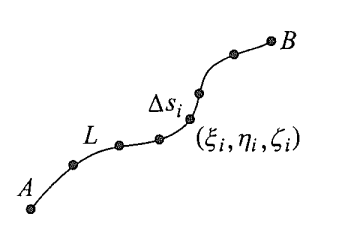
\includegraphics[width=\textwidth]{2.1.png} % 无需重复指定宽度  
\end{myimagebox}     
\caption{\label{fig:2.1}第一型曲线积分的定义}   
\end{figure}

我们考虑一条绳子,绳子上任意一点$M(x,y,z)$的线密度为$\rho(x,y,z)$,我们利用微元法可以计算出绳子的质量为:
\begin{align*}
    m=\int_L \rho(x,y,z)\mathrm{d}s\tag{2-1}
\end{align*}

这就是\textbf{\color{brown!50!red}沿着曲线$L$的第一型曲线积分}。$\mathrm{d}s$是\textbf{\color{brown!50!red}弧微元}。曲线$L$是\textbf{\color{brown!50!red}积分曲线}。

对于2-1有意义,则则弧微分要存在,也就是说这条曲线要\textbf{\color{brown!50!red}分段光滑}。那么我们可以将曲线进行参数化定义连续性。令曲线L有$x=x(t),y=y(t),z=z(t)$。则第一型曲线积分存在的\textbf{\color{brown!50!red}充分必要条件}为$x(t),y(t),z(t)\in C^1[a,b]$。
\begin{tcolorbox}[
    colback=bac2,     % 极浅黄色背景
    colframe=fra2,   % 浅黄色边框
    coltitle=white,             % 标题文字白色
    coltext=tex2,
    title=第一型曲线积分的性质,
    fonttitle=\bfseries,        % 标题加粗
arc=3mm,                     % 圆角稍大
breakable
]
第一型曲线积分有一些性质。分别是:

\textbf{\color{brown!50!red}线性性}:$\int_L(af+bg)\mathrm{d}s=a\int_Lf\mathrm{d}s+b\int_Lg\mathrm{d}s$

\textbf{\color{brown!50!red}分段可加性}:设$L=L_1\cup L_2,S(L_1\cap L_2)=\Phi $,则有$\int_L f\mathrm{d}s=\int_{L_1}f\mathrm{d}s+\int_{L_2}\mathrm{d}s$

\textbf{\color{brown!50!red}无方向性}:设$R$是$L$逆向曲线,则$\int_L f\mathrm{d}s=\int_R f\mathrm{d}s$
\end{tcolorbox}

\subsubsection{第一型曲线积分的计算}
在式子2-1中,进一步就是对于弧微分的化简。假如我们将曲线全部参数化,根据高数(I)的结论,则:
\begin{tcolorbox}[
    colback=bac1,     % 极浅黄色背景
    colframe=fra1,   % 浅黄色边框
    coltitle=white,             % 标题文字白色
    coltext=tex1,
    title=第一型曲线积分的计算,
    fonttitle=\bfseries,        % 标题加粗
arc=3mm,                     % 圆角稍大
breakable
]
第一型曲线计算方法为:
\begin{align*} 
\int_L\rho(x,y,z)\mathrm{d}s=\int_L\rho(x(t);y(t);z(t))\sqrt{x'(t)^2+y'(t)^2+z'(t)^2}\mathrm{d}t
\tag{2-2}  
\end{align*}

一般地对于一个二维平面的曲线$y=y(x)$,式子2-2会简化成:
\begin{align*} 
\int_Ly(x)\mathrm{d}s=\int_Ly(x)\sqrt{y'(x)^2+1}\mathrm{d}x
\tag{2-3} 
\end{align*}
\end{tcolorbox}

第一型曲线积分可以\textbf{\color{brown!50!red}求弧长}。只需要对1积分即可。

\textbf{\color{brown!50!red}例}:计算$\int_L xy^2\mathrm{d}s$,其中$L$为$\Delta OAB$的边界,$O(0,0),A(0,1),B(1,1)$。

\textbf{\color{brown!50!red}解}:令$L_1=OA,L_2=AB,L_3=BO$,分开进行积分即可。
\begin{align*} 
\int_{L_1}xy^2\mathrm{d}s&=\int_0^1x\times0\mathrm{d}s=0\\
 \int_{L_2}xy^2\mathrm{d}s&=\int_0^1 y^2\mathrm{d}y=\frac{1}{3}\\
\int_{L_3}xy^2\mathrm{d}s&=\int_0^1y^3\sqrt{2}\mathrm{d}y=\frac{\sqrt{2}}{4}\\
I&=\frac{1}{3}+\frac{\sqrt{2}}{4}
\end{align*}

\textbf{\color{brown!50!red}例}:当曲线复杂的时候,可能第一型曲线积分的计算会有一些困难。求$I=\oint_C x^2\mathrm{d}s$,其中$C$是平面$x^2+y^2+z^2=R^2,x+y+z=0$的交线。

\textbf{\color{brown!50!red}解}:这是一个平面和球面的交线,因此\textbf{\color{brown!50!red}它是空间的一个圆周(在$Oxy$平面的投影是一个椭圆)}。将$z=-x-y$代入球面,得到$x^2+y^2+z^2=\frac{R^2}{2}$,配方法得到:
\begin{align*}
    \left(\frac{\sqrt{3}}{2}x\right)^2+\left(\frac{x}{2}+y\right)^2=\frac{R^2}{2}
\end{align*}

因此令$\frac{\sqrt{3}}{2}x=\frac{R}{\sqrt{2}}\cos t$,令$\frac{x}{2}+y=\frac{R}{\sqrt{2}}\sin t$,则$z=-\frac{R}{\sqrt{6}}\cos t-\frac{R}{\sqrt{2}}\sin t$,因此弧微分有:
\begin{align*} 
\mathrm{d}s&=\sqrt{x'(t)^2+y'(t)^2+z'(t)^2}\mathrm{d}t\\
&=\sqrt{\frac{2}{3}\sin^2t+(\frac{\cos t}{\sqrt{2}}+\frac{\sin t}{\sqrt{6}})^2
+ (-\frac{\cos t}{\sqrt{2}}+\frac{\sin t}{\sqrt{6}})^2 }\mathrm{d}t\\
&=R\mathrm{d}t
\end{align*}

因此代入就有:
\begin{align*} 
I=\int_0^{2\pi}\frac{2}{3}R^3\cos^2t\mathrm{d}t=\frac{2}{3}\pi R^3   
\end{align*}

\subsection{第二型曲线积分}
\subsubsection{第二型曲线积分的定义}
\begin{figure}[H]    
\centering     
\renewcommand{\figurename}{图}     
\renewcommand{\thefigure}{2.2}    
\begin{myimagebox}[width=0.39\textwidth] % 直接传入图片尺寸参数      
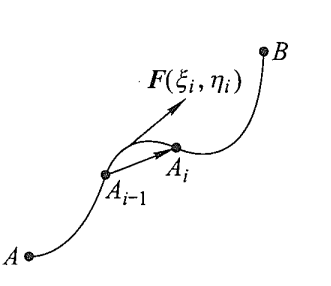
\includegraphics[width=\textwidth]{2.2.png} % 无需重复指定宽度  
\end{myimagebox}     
\caption{\label{fig:2.2}第二型曲线积分的定义}   
\end{figure}

我们考虑一个物理问题:给定三维空间中光滑曲线$L$和一个正方向。设一个点$P$从$A$点运动到$B$点,沿途受力为向量$\bm{F}(x,y,z)$,求力做的功。

那么根据微元法,先进行分割,则微元功为$\Delta W_i=|\bm{F}||\bm{A_{i-1}A_i}|\cos\theta=\bm{F_i}\cdot \bm{r_i}$。然后进行积分取极限可得:
\begin{align*}
W=\int_{\bm{AB}}\bm{F}\mathrm{d}\bm{r}\tag{2-4}
\end{align*}

第二型曲线积分具有线性性和分段可加性。但与第一型曲线积分不同的是,它具有有向性。

\subsubsection{第二型曲线积分的计算}
\begin{tcolorbox}[
    colback=bac1,     % 极浅黄色背景
    colframe=fra1,   % 浅黄色边框
    coltitle=white,             % 标题文字白色
    coltext=tex1,
    title= 第二型曲线积分的计算,
    fonttitle=\bfseries,        % 标题加粗
arc=3mm,                     % 圆角稍大
breakable
]
如果说给出了直角坐标系$\bm{F}$的解析式$\bm{F}=(P(x,y,z),Q(x,y,z),R(x,y,z))$,由于$\mathrm{d}\bm{r}=(\bm{d}x,\bm{d}y,\bm{d}z)$。根据向量点乘与式子2-4的左侧可以得到:
\begin{align*} 
\int_{\bm{AB}}\bm{F}\mathrm{d}\bm{r}=
\int_{\bm{AB}}P\mathrm{d}x+Q\mathrm{d}y+R\mathrm{d}z\tag{2-5}  
\end{align*}

那么曲线参数化的时候会变成什么样?给定有向曲线L的方程为$x(t),y(t),z(t),t\in[\alpha,\beta]$,且参数方程都一阶连续可导,则有:
\begin{align*}  \int_{\bm{AB}}\bm{F}\mathrm{d}\bm{r}=
\int_{\bm{AB}}\left[P(t)x'(t)+Q(t)y'(t)+R(t)z'(t)\right]\mathrm{d}t\tag{2-6} 
\end{align*}
\end{tcolorbox}

\textbf{\color{brown!50!red}例}:计算积分$I=\int_C (x^2+2xy)\mathrm{d}y$,其中积分曲线为逆时针方向的上半椭圆$\frac{x^2}{a^2}+\frac{y^2}{b^2}=1$

\textbf{\color{brown!50!red}解}:利用参数方程$x=a\cos t,y=b \sin t,t\in[0,\pi]$,可以进行计算。
\begin{align*}
   I&=\int_C (x^2+2xy)\mathrm{d}y=\int_0^\pi(a^2\cos^2t+2a^2\cos t\sin t)b\cos t\mathrm{d}t \\
&=a^2b\left ( \int_0^\pi\cos^3 t\mathrm{d}t+2\int_0^\pi\cos^2 t\sin t\mathrm
d t \right )\\
&=a^2b(\frac{2}{3}+ \frac{2}{3})=\frac{4}{3}a^2b 
\end{align*}

\textbf{\color{brown!50!red}例}:计算积分$\int_L(x+y^3)\mathrm{d}x+3xy^2\mathrm{d}y,A(0,1),B(1,0),C(1,1)$。积分路径$L$分别为折线段$ACB$与圆弧$AB$。

\textbf{\color{brown!50!red}解:}对于第一种情况,应该为$I_1=\int_0^1(x+1)\mathrm{d}x+\int_1^03y^2\mathrm{d}y=\frac{1}{2}$。

对于第二种情况,令$x=\cos t,y=\sin t,t\in[\pi,0]$,进行换元计算,答案也是$\frac{1}{2}$。

巧合的是,这两个积分的值是一样的,这个积分与积分路径无关。这背后的原因我们会在下个部分解释。

\subsubsection{两种曲线积分的联系}
假设曲线参数化,则2-6中$\mathrm{d}\bm{r}=(x',y',z'),|\mathrm{d}\bm{r}|=\mathrm{d}s$。而又根据方向余弦的定义有:
\begin{align*}
   \frac{\mathrm{d}\bm{r} }{|\mathrm{d}\bm{r} |} =(\cos\alpha ,\cos\beta ,\cos\gamma ) =(\frac{\mathrm{d}x}{\mathrm{d}s},\frac{\mathrm{d}y}{\mathrm{d}s},\frac{\mathrm{d}z}{\mathrm{d}s})\tag{2-7}
\end{align*}

因此,$\mathrm{d}x=\cos\alpha\mathrm{d}s$,带换到2-5可得:
\begin{align*}
\int_{\bm{AB}}P\mathrm{d}x+Q\mathrm{d}y+R\mathrm{d}z=
\int_{\bm{AB}}[P\cos\alpha+Q\cos\beta+R\cos\gamma ]\mathrm{d}s\tag{2-8} 
\end{align*}

我们要注意,这个方向余弦是\textbf{\color{brown!50!red}曲线切线}和\textbf{\color{brown!50!red}各个坐标轴的余弦值}。因此进行转化的时候,本质上就是要求出\textbf{\color{brown!50!red}方向余弦值}的大小

\textbf{\color{brown!50!red}例}:将第二型曲线积分$I=\int_L y\mathrm{d}x+x\mathrm{d}y+xyz\mathrm{d}z$转化成第一型曲线积分。其中曲线$L$的参数方程为$x=2t,y=t^2,z=t-1,t\in[0,1]$。

\textbf{\color{brown!50!red}解}:先找曲线的切线向量,为$(2,2t,1)$。然后计算方向余弦,$\cos\alpha=\frac{2}{\sqrt{5+4t^2}}=\frac{2}{\sqrt{5+4y^2}},\cos\beta=\frac{2t}{\sqrt{5+4t^2}}=\frac{x}{\sqrt{5+4y^2}},\cos\gamma=\frac{1}{\sqrt{5+4y^2}}$,然后代入2-8即可。

\subsection{格林公式}
\subsubsection{格林公式的内容}
格林公式的本质就是把\textbf{\color{brown!50!red}平面上的第二型曲线积分转化成二重积分}。为了引入这一公式,我们需要先引入几个概念。

我们定义平面简单闭合曲线(\textbf{\color{brown!50!red}Jordan曲线}):是、有映射$\phi[\alpha,\beta]\to \mathbb{R}^2,\phi(t)=(x(t),y(t)),\phi\in C[\alpha,\beta]$且单射,$\phi(\beta)=\phi(\alpha)$的曲线。从集合上看就是\textbf{\color{brown!50!red}首尾重合且其他地方不相交的曲线}。

一条Jordan曲线把平面分成有界部分和无界部分(Jordan定理)。我们定义有界部分是Jordan曲线的\textbf{\color{brown!50!red}内部}。

现在我们来定义单连通区域:设平面区域D内任意一条Jordan曲线内部都包含于区域D中,称区域D为\textbf{\color{brown!50!red}单连通区域}。

接下来我们为Jordan曲线确定方向。设二维有界区域D的边界$\partial$D由一条或多条Jordan曲线组成,则定义$\Gamma$的正方向如下:设正向移动时区域D的内部总在转动方向左侧,把正方向记作$\Gamma^+$
\begin{figure}[H]    
\centering     
\renewcommand{\figurename}{图}     
\renewcommand{\thefigure}{2.3}    
\begin{myimagebox}[width=0.7\textwidth] % 直接传入图片尺寸参数      
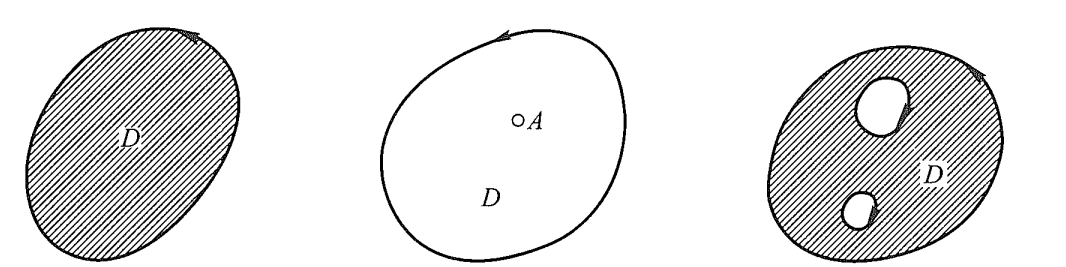
\includegraphics[width=\textwidth]{2.3.png} % 无需重复指定宽度  
\end{myimagebox}     
\caption{\label{fig:2.3}单连通区域的正向曲线}   
\end{figure}

在这个图中,只有左边的区域为单连通区域,其余的是多连通区域。正方向如图中所表示。

接下来我们介绍\textbf{\color{brown!50!red}格林公式}:
\begin{tcolorbox}[
    colback=bac2,     % 极浅黄色背景
    colframe=fra2,   % 浅黄色边框
    coltitle=white,             % 标题文字白色
    coltext=tex2,
    title=Green格林公式,
    fonttitle=\bfseries,        % 标题加粗
arc=3mm,                     % 圆角稍大
breakable
]
设二维有界区域$D$的边界由一条或多条Jordan曲线围成,令$\bm{F}(x,y)=(P(x,y),Q(x,y)\in C^1(D)$,则有:
\begin{align*}
\oint_{\Gamma^+}\bm{F}\mathrm{d}\bm{r}=\iint_D (\frac{\partial  Q}{\partial  x}-
\frac{\partial P}{\partial  y}  )\mathrm{d}x\mathrm{d}y\tag{2-9}  
\end{align*}
\end{tcolorbox}

Green公式的证明,只需要我们去证明
\begin{align*}
  \oint_{\Gamma^+}P\mathrm{d}x&=\iint -P_y\mathrm{d}x\mathrm{d}y\tag{2-10}\\
  \oint_{\Gamma^+}Q\mathrm{d}y&=\iint Q_x\mathrm{d}x\mathrm{d}y  
\end{align*}

这两个式子的证明方式是一样的,我们只证明第一个式子即可。

我们从单连通区域先入手,单连通区域也从最特殊的情况先入手。
\begin{figure}[H]    
\centering     
\renewcommand{\figurename}{图}     
\renewcommand{\thefigure}{2.4}    
\begin{myimagebox}[width=0.3\textwidth] % 直接传入图片尺寸参数      
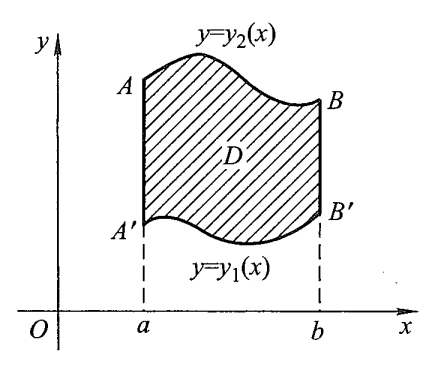
\includegraphics[width=\textwidth]{2.4.png} % 无需重复指定宽度  
\end{myimagebox}     
\caption{\label{fig:2.4}单连通区域的Green公式}   
\end{figure}

这个区域是由$y=y_1(x),y=y_2(x),x=a,x=b$围成。则2-10等式左侧可以计算为:
\begin{align*}
\oint_{\Gamma^+}P\mathrm{d}x&=\int_{\stackrel\frown{A'B'}}P\mathrm{d}x+
\int_{\stackrel\frown{B'B}}P\mathrm{d}x+\int_{\stackrel\frown{BA}}P\mathrm{d}x+
\int_{\stackrel\frown{AA'}}P\mathrm{d}x\\
&=\int_a^bP(x,y_1(x))\mathrm{d}x+0+\int_b^aP(x,y_2(x))\mathrm{d}x+0  
\end{align*}

另一方面,根据二重积分计算方法,2-10右侧可写成:
\begin{align*}
\iint_D-\frac{\partial  P}{\partial  y}\mathrm{d}x\mathrm{d}y&=\int_a^b\mathrm{d}x\int_{y_1(x)}
^{y_2(x)}  -\frac{\partial  P}{\partial  y}\mathrm{d}y\\
&=-\int_a^b[P(x,y_2(x))-P(x,y_1(x))]\mathrm{d}x\\
&=\int_a^bP(x,y_1(x))\mathrm{d}x+\int_b^aP(x,y_2(x))\mathrm{d}x
\end{align*}

因此2-10证毕,这也就是说在这种情况下Green公式成立。在复杂的单连通区域中,我们可以割成多个这样的单连通区域。

对于一般的多连通区域,我们继续割成多个单连通区域,如图2.5。
\begin{figure}[H]    
\centering     
\renewcommand{\figurename}{图}     
\renewcommand{\thefigure}{2.5}    
\begin{myimagebox}[width=0.7\textwidth] % 直接传入图片尺寸参数      
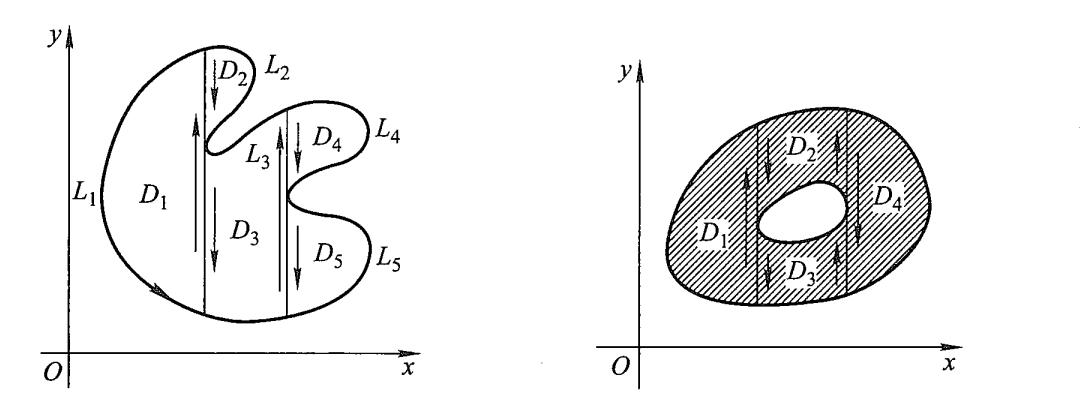
\includegraphics[width=\textwidth]{2.5.png} % 无需重复指定宽度  
\end{myimagebox}     
\caption{\label{fig:2.5}多连通区域的Green公式}   
\end{figure}

在这种情况下,我们发现\textbf{\color{brown!50!red}分割线上的积分相互抵消}。剩下的积分就是区域的正向曲线上的积分。因此Green公式继续成立。

接下来我们利用2-9和2-8证明一个很重要的命题:
\begin{tcolorbox}[
    colback=bac1,     % 极浅黄色背景
    colframe=fra1,   % 浅黄色边框
    coltitle=white,             % 标题文字白色
    coltext=tex1,
    title=Green公式推论,
    fonttitle=\bfseries,        % 标题加粗
arc=3mm,                     % 圆角稍大
breakable
]
给定向量函数$\bm{F}(x;y)=(P(x;y),Q(x;y))\in C^1(D)$,且$\bm{n}$为边界的单位外法向量。则:
\begin{align*}
\oint_{\Gamma}\bm{F}\cdot\bm{n}\mathrm{d}s=\iint_D(\frac{\partial  P}{\partial x}
+\frac{\partial  Q}{\partial  y}  )\mathrm{d}x\mathrm{d}y\tag{2-11}   
\end{align*}

根据Green公式与式子2-8,则有:
\begin{align*}
\iint_D(\frac{\partial  P}{\partial x}
+\frac{\partial  Q}{\partial  y}  )\mathrm{d}x\mathrm{d}y&=
\oint_{\Gamma^+}-Q\mathrm{d}x+P\mathrm{d}y \\
&=\oint_{\Gamma^+}[Q\sin(x,\mathrm{n} )+P\cos(x,\bm{n}) ]\mathrm{d}s 
\end{align*}

而在几何上容易得到$\sin(x,\bm{n})=\cos(y,\bm{n})$,证毕。在2-11中,右侧的积分函数称作\textbf{\color{brown!50!red}散度}。
\end{tcolorbox}

\textbf{\color{brown!50!red}例}:曲线$C$是抛物线$2x=\pi y^2,O(0,0)\to B(\frac{\pi}{2},1)$的弧段,求积分:
\begin{align*}
I=\int_C(2xy^3-y^2\cos x)\mathrm{d}x+(1-2y\sin x+3x^2y^2)\mathrm{d}y  
\end{align*}

第一种办法是根据之前的办法计算。第二种是Green公式。但这不是一个闭合味道。因此我们选取点$A(\frac{\pi}{2},0)$,取围道$OBAO$。由于:
\begin{align*}
\frac{\partial  Q}{\partial  x}-
\frac{\partial P}{\partial  y}  =0
\end{align*}

因此整体是0。也就是说,I的值也可以根据积分路径$OAB$计算。且$OA$路径上$y=0$,积分为0.因此:
\begin{align*}
I=\int_0^1(1-2y+3(\frac{\pi}{2})^2y)\mathrm{d}y=\frac{\pi^2}{4}   
\end{align*}

\textbf{\color{brown!50!red}例}:计算积分:
\begin{align*}
I=\oint_C\frac{e^y}{x^2+y^2}[(x\sin x+y\cos x)\mathrm{d}x+(y\sin x-x\cos x)\mathrm{d}y]   
\end{align*}
$C$的边界不过原点,是平面内任意一条Jordan曲线。

\textbf{\color{brown!50!red}解}:Green公式的使用条件是\textbf{\color{brown!50!red}P、Q在区域内连续可微}。在这里,令:
\begin{align*}
P(x,y)=\frac{e^y}{x^2+y^2}(x\sin x+y\cos x)\qquad Q(x,y)=\frac{e^y}{x^2+y^2}(y\sin x-x\cos x) 
\end{align*}

显然这两个函数在原点不是连续可微的,因此需要分类讨论。当原点不在区域内的时候,可以直接构建Green函数公式,由于$\partial{Q}/\partial{x}-\partial{P}/\partial{y}=0$,则积分直接为0。

当原点在区域内的时候,选择围道$C_\varepsilon:x^2+y^2=\varepsilon^2$,逆时针方向。则$I=\oint_C-\oint_{C_\varepsilon}+\oint_{C_\varepsilon}=\oint_{C_\varepsilon}$,因此:
\begin{align*}
I&= \oint_{C_\varepsilon}\frac{e^y}{x^2+y^2}[(x\sin x+y\cos x)\mathrm{d}x+(y\sin x-x\cos x)\mathrm{d}y]\\
&=\frac{1}{\varepsilon ^2} \oint_{C_\varepsilon}e^y[(x\sin x+y\cos x)\mathrm{d}x+(y\sin x-x\cos x)\mathrm{d}y]
\end{align*}

此时对于里面的函数,可以使用Green公式了,因此使用Green公式并进行一次积分中值定理:
\begin{align*}
I&=\frac{1}{\varepsilon ^2} \iint_{D}-2e^y\cos x\mathrm{d}x\mathrm{d}y\\
&=\frac{1}{\varepsilon ^2}(-2\pi \varepsilon ^2e^\eta\cos\xi)\\
&=-2\pi e^\eta\cos\xi 
\end{align*}

由于这是对任意的$\epsilon>0$都成立,因此当$\varepsilon\to 0$时,$I\to -2\pi$,即就是答案。

我们接下来再看一个问题。给定D为单连通有界闭区域,且函数$u=u(x,y)\in C^2(D),\nabla u=(u_x,u_y)=(P,Q)$。证明:
\begin{align*}
\oint_{\Gamma^+}(\nabla u\cdot \bm{n})\mathrm{d}s=\iint_D\Delta u\mathrm{d}x\mathrm{d}y   
\qquad (\Delta u=u_{xx}+u_{yy})\tag{2-12}
\end{align*}

这个题直接带入式子2-11即可。这个是式子有着非常多的应用的。例如:如果函数$f$在区域D满足$\Delta f=0$以及边界$\Gamma$上满足$f=0$,则在整个区域D上满足$f\equiv 0$。

\textbf{\color{brown!50!red}证明}:令$u=f^2$,则有:
\begin{align*}
\nabla u=2f\nabla f&\qquad\Delta u=2f\Delta f+2\nabla f\cdot\nabla f\\
\iint_D\Delta u\mathrm dx\mathrm{d}y&=0=\iint_D(2f\Delta  f +2\nabla f\cdot\nabla f)\mathrm dx\mathrm{d}y\\
&=2\iint_D\nabla f\cdot\nabla f \mathrm dx\mathrm{d}y\\
&=2\iint_D(f_{x}^2+f_{y}^2)\mathrm{d}x\mathrm{d}y
\end{align*}

我们指出,式子为0这一步是利用了式子2-12的左侧,因为在边界上$\nabla u=2f\nabla f=0\nabla f$,因此$\nabla u$在边界上是0向量。因此我们可以得到在区域内$f_x=0,f_y=0$,即就是$f\equiv C$。而在边界上取值为0,一次在整个区域内$f\equiv 0$。证毕。
\begin{tcolorbox}[
    colback=bac2,     % 极浅黄色背景
    colframe=fra2,   % 浅黄色边框
    coltitle=white,             % 标题文字白色
    coltext=tex2,
    title=多说一点,
    fonttitle=\bfseries,        % 标题加粗
arc=3mm,                     % 圆角稍大
breakable
]
因此这个问题可以进一步扩展到,给定区域$D$与边界$\Gamma$,有$\Delta f=g(D),f=h(\Gamma)$。则这个解是唯一的(提示:利用反证法,二者相减即可证明)。
\end{tcolorbox}

\subsubsection{积分与积分路径无关}
在什么时候第二型曲线积分的积分路径和积分值无关?根据Green公式的性质,我们可以得到结论:
\begin{tcolorbox}[
    colback=bac2,     % 极浅黄色背景
    colframe=fra2,   % 浅黄色边框
    coltitle=white,             % 标题文字白色
    coltext=tex2,
    title=积分与路径无关,
    fonttitle=\bfseries,        % 标题加粗
arc=3mm,                     % 圆角稍大
breakable
]
设D为单连通区域,$(P,Q)\in C^1 (D)$,则\textbf{\color{brown!50!red}任意曲线积分与路径无关的充要条件是在区域D内有}:
\begin{align*}
\frac{\partial  Q}{\partial  x}-
\frac{\partial P}{\partial  y}  =0\tag{2-13}
\end{align*}
\end{tcolorbox}

从右往左证明很简单,选择积分围道即可。从左往右证明可以利用反证法。不妨$\exists (x_0,y_0)\in D^*,(Q_x-P_y)=a>0$,则$\exists D_1\subseteq D$,使得$Q_x-P_y>\frac{a}{2}$二重积分的值$ I \geq \frac{aS}{2}>0 $,矛盾。

当然,证明与路径无关还有其他定理。2-13成立的充分条件是:存在函数$u(x,y)$,满足:
\begin{align*}
\mathrm{d}u=P\mathrm{d}x+Q\mathrm{d}y  \tag{2-14}
\end{align*}

充分性证明很简单,直接求导即可。必要性则是证明2-13成立可推导至2-14成立。2-13成立说明积分与路径无关。我们固定积分起点$(x_0,y_0)$,则曲线积分的值就是积分终点$(x,y)$的函数。令积分大小为$u(x;y)$,即就是:
\begin{align*}
u(x;y)=\int_{(x_0,y_0)}^{(x,y)}P\mathrm{d}x+Q\mathrm{d}y   
\end{align*}

我们只需证明$u_x=P$即可。另一侧是一样的。两边求微分:
\begin{align*}
u(x+\Delta x,y)-u(x,y)&=\int_x^{x+\Delta x}P\mathrm{d}x=P(\xi,y)\Delta x\\  
\lim_{\Delta x\to 0} \frac{u(x+\Delta x,y)-u(x,y)}{\Delta x}&=\lim_{\Delta x\to 0} P(\xi,y)=P(x,y)
\end{align*}

我们得到了一个副产物:$u$就是\textbf{\color{brown!50!red}积分值}。因此我们得到第二型曲线积分的另一种计算方法:
\begin{align*}
\int_{\bm{AB}}P\mathrm{d}x+Q\mathrm{d}y=u(B)-u(A)\tag{2-15} 
\end{align*}

\subsection{习题补充与拓展}
\textbf{\color{brown!50!red}例1}:计算下面的积分:
\begin{align*}
&(1)\int_C (x^{\frac{4}{3} }+y^{\frac{4}{3} })\mathrm{d}s \qquad 
C:x^{\frac{2}{3} }+y^{\frac{2}{3} }=a^\frac{2}{3}\\ 
&(2)\int_C |y|\mathrm{d}s\qquad C:(x^2+y^2)^2=a^2(x^2-y^2) 
\end{align*}

解:第一题进行曲线参数化,记$x=a\cos^3\theta,y=a\cos^3\theta$。则弧微分可表示为:
\begin{align*}
\mathrm{d}s&=\sqrt{(-3a\cos^2\theta\sin\theta)^2+(3a\sin^2\theta\cos\theta)^2}\mathrm{d}\theta \\
&=3a\sin\theta\cos\theta\mathrm{d}\theta 
\end{align*}
因此原式可以写成:
\begin{align*}
I&=\int_0^{2\pi}a^{\frac{4}{3} }(\cos^4\theta+\sin^3\theta)3a\sin\theta\cos\theta\mathrm{d}\theta \\
&=4a^{\frac{7}{3}}
\end{align*}

第二题似乎不太好进行参数化,我们使用极坐标方程$x=r\cos\theta,y=r\sin\theta$,代换得到$r^2=a^2\cos{2\theta}$。\textbf{\color{brown!50!red}极坐标下的弧微元计算方法如下}:
\begin{align*}
\mathrm{d}s&=\sqrt{r^2+(r')^2}\mathrm{d}\theta = \frac{a}{\sqrt{\cos 2\theta}}\mathrm{d}\theta\tag{2-16}  \\
I&=4\int_0^{\frac{\pi}{4} }a\sqrt{\cos2\theta}\sin\theta\frac{a}{\sqrt{\cos 2\theta}}\mathrm{d}\theta\\
&=-4a^2\cos\theta|_0^{\frac{\pi}{4} }\\
&=2a^2(2-\sqrt{2})
\end{align*}

\textbf{\color{brown!50!red}例2}:在第一型曲线积分中,对于式子2-2,如果把曲线拓展到多维空间,则曲线$\Gamma: \bm{x}=\bm{x}(t)\in\mathbb{R}^n$。则第一型曲线积分的表达式为:
\begin{align*}
    \int_L f(x)\mathrm{d}s=\int_a^bf(x(t))|x(t)'|\mathrm{d}t
\end{align*}

那么设曲线$\Gamma=\widetilde{AB}$是n维空间的简单可求长度的曲线,弧长记作L,对每一个$s\in[0,L]$,均存在唯一的$\bm{x}\in\Gamma,\bm{x}=(x_1,x_2,...,x_n)$,使得曲线上从A到这一点的曲线段的弧长为$s$,因此我们定义了一个函数$\bm{x}=\bm{x}(s),0\leq s\leq L$。这就是\textbf{\color{brown!50!red}曲线以弧长$s$为参数的参数方程}。设$f$是定义在曲线的函数,如果$f$在曲线上的第一型曲线积分存在,证明:
\begin{align*}
f(\bm{x} )\mathrm{d}s=\int_0^Lf(\bm{x} (s))\mathrm{d}s   
\end{align*}

\textbf{\color{brown!50!red}解}:记$a=s^{-1}(0),b=s^{-1}(L)$,则根据表达式则有:
\begin{align*}
|\bm{x}'(t)|&=s'(t)=\frac{\mathrm{d}s(t) }{\mathrm{d}t } \\
|\bm{x}'(s)|&=\frac{\mathrm{d}s }{\mathrm{d}s }=1   
\end{align*}

因此就有:
\begin{align*}
\int_a^b f(x(t))|x'(t)|\mathrm{d}t=\int_0^Lf(x(s))|x'(s)|\mathrm{d}s=\int_0^Lf(x(s))\mathrm{d}s  
\end{align*}

\textbf{\color{brown!50!red}例3}:计算第二型曲线积分
\begin{align*}
\oint_C (y^2+z^2)\mathrm{d}x+(z^2+x^2)\mathrm{d}y+(x^2+y^2)\mathrm{d}z
\end{align*}
其中$C$是曲面$x^2+y^2+z^2=2Rx,x^2+y^2=2ax,0<a<R,z>0$的交线。且从z轴正向看是逆时针方向。

\textbf{\color{brown!50!red}解}:采用柱坐标换元。则联立曲线则有:
\begin{align*}
z^2+r^2=2Rr\cos\theta\qquad r^2=2ar\cos\theta\\
x=2a\cos^2\theta\quad y=2a\sin\theta\cos\theta\quad  z=\sqrt{4a\cos^2\theta(R-a)} 
\end{align*}

根据$z>0$,可以得到$\theta\in[-\frac{\pi}{2},\frac{\pi}{2}]$。因此原积分可以写作:
\begin{align*}
I&=\oint_C (y^2+z^2)\mathrm{d}x+(z^2+x^2)\mathrm{d}y+(x^2+y^2)\mathrm{d}z\\
&=\int_{-\frac{\pi}{2}}^{\frac{\pi}{2} }(4a^2\sin^2\theta\cos^2\theta+4a\cos^2\theta(R-a))(-4a\cos\theta\sin\theta)
\mathrm{d}\theta+\\
& \int_{-\frac{\pi}{2}}^{\frac{\pi}{2} }(4a\cos^2\theta(R-a)+4a^2\sin^2\theta\cos^2\theta)(2a\cos 2\theta)
\mathrm{d}\theta+\int_{-\frac{\pi}{2}}^{\frac{\pi}{2} }(4a^2\cos^2\theta)z'(\theta)\mathrm{d}\theta 
\end{align*}

由于第一项和第三项的\textbf{\color{brown!50!red}被积函数都是奇函数},因此积分值直接为0,因此:
\begin{align*}
I&=\int_{-\frac{\pi}{2}}^{\frac{\pi}{2} }(4a\cos^2\theta(R-a)+4a^2\sin^2\theta\cos^2\theta)(2a\cos 2\theta)
\mathrm{d}\theta\\
&=8a^2\int_{-\frac{\pi}{2}}^{\frac{\pi}{2} }(-a\cos^4\theta+R\cos^2\theta)\cos2\theta\mathrm{d}\theta\\
&=2a^2R\pi 
\end{align*}

\textbf{\color{brown!50!red}例4}:解下列积分。

(1)$\oint_C\frac{\partial u}{\partial \bm{n}}\mathrm{d}s$,其中$u=x^2+y^2,C;x^2+y^2=6x,\bm{n}$为曲线上的单位外法向量。

(2) 设$C$为逐段光滑的简单闭曲线,$l$为给定方向。证明$\oint_C \cos(\bm{l},\bm{n})=0$,其中$\bm{n}$是曲线上的单位外法向量。

\textbf{\color{brown!50!red}解}:考虑到方向导数的定义,则有:
\begin{align*}
\frac{\partial  u}{\partial  \bm{n}}&=\frac{\partial u}{\partial x}\cos(n,x)+\frac{\partial u}
{\partial y}\cos(n,y) \\
\frac{\partial  u}{\partial  \bm{n}}\mathrm{d}s &=\frac{\partial u}{\partial x}\mathrm{d}y -\frac{\partial u}
{\partial y}\mathrm{d}x \\
I&=\iint_D(\frac{\partial^2 u}{\partial x^2} +\frac{\partial^2 u}
{\partial y^2})\mathrm{d}x\mathrm{d}y\\&=\iint_D 4\mathrm{d}x\mathrm{d}y=36\pi 
\end{align*}

对于第二题,我们先定义$\bm{t}$表示单位切向量,$\bm{n}$为单位法向量,如下图所示。
\begin{figure}[H]    
\centering     
\renewcommand{\figurename}{图}     
\renewcommand{\thefigure}{2.6}    
\begin{myimagebox}[width=0.5\textwidth] % 直接传入图片尺寸参数      
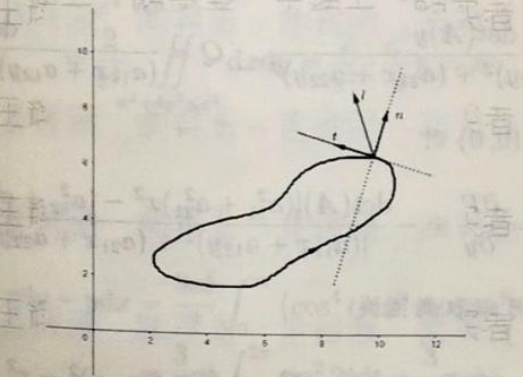
\includegraphics[width=\textwidth]{2.6.png} % 无需重复指定宽度  
\end{myimagebox}     
\caption{\label{fig:2.6}例4第二题示意图}   
\end{figure}

一方面,我们可以注意到,
\begin{align*}
(l,n)&=(l,x)-(n,x)\\
\cos(l,n)&=\cos(l,x)\cos(n,x)+\sin(l,x)\sin(n,x)
\end{align*}

另一方面,由于
\begin{align*}
\sin(n,x)&=-\cos(t,x)=-\frac{\mathrm{d}x}{\mathrm{d}s}\\
\cos(n,x)&=\sin(t,x)=\frac{\mathrm{d}y}{\mathrm{d}s}
\end{align*}

因此有:
\begin{align*}
\cos(l,n)\mathrm{d}s=\cos(l,x)\mathrm{d}y-\sin(l,x)\mathrm{d}x   
\end{align*}

而$l$方向给定,因此$\cos(l,x),\sin(l,x)$是定值。因此根据Green公式则有:
\begin{align*}
I=\oint_C\cos(l,x)\mathrm{d}y-\sin(l,x)\mathrm{d}x =\iint_D 0\mathrm{d}x\mathrm{d}y=0    
\end{align*}

\textbf{\color{brown!50!red}例5}:设$u(x;y)$在平面空间上连续。证明:
\begin{align*}
    u(x,y)=\frac{1}{\pi r^2}\iint_{(x-\xi)^2+(y-\eta)^2\leq r^2}u(\xi,\eta)\mathrm{d}\xi\mathrm{d}\eta
\end{align*}

对于$\forall r>0$成立的必要条件是
\begin{align*}
     u(x,y)=\frac{1}{2\pi r}\oint_{(x-\xi)^2+(y-\eta)^2\leq r^2}u(\xi,\eta)\mathrm{d}s
\end{align*}

对于$\forall r>0$成立。

\textbf{\color{brown!50!red}解}:进行极坐标换元$\xi=x-\rho\cos\theta$,$\eta=y-\rho\sin\theta$,将第一个式子化简即得:
\begin{align*}
    \pi r^2 u(x,y)=\int_0^{2\pi}\mathrm{d}\theta\int_0^r \rho u(x-r\cos\theta,y-r\sin\theta)\mathrm{d}\rho
\end{align*}

根据这个积分的收敛性,两边对r求导后,右边可以直接对积分函数求导,则有:
\begin{align*}
    2\pi r u(x,y)=\int_0^{2\pi} r u(x-r\cos\theta,y-r\sin\theta)\mathrm{d}\theta
\end{align*}

而把第一型曲面积分转化为定积分也是这个答案。

\textbf{\color{brown!50!red}例6}:证明两个不等式。

(1)设$L$是曲线$C$的弧长,定义$M=\max_{(x,y)\in C}\{\sqrt{P(x,y)^2+Q(x,y)^2}\}$,证明:
\begin{align*}
    \left | \int_CP(x,y)\mathrm{d}x+Q(x,y)\mathrm{d}y\right | \leq ML  
\end{align*}

(2) 设$f(x;y)$在区域G上连续一阶可微。在$\partial G$有$f=0,G=\{x^2+y^2=a^2\}$,证明:
\begin{align*}
    \left | \iint_Gf(x,y)\mathrm{d}x\mathrm{d}y\right | \leq \frac{\pi}{3}a^3\max_G\{(f_x^2+f_y^2)^{\frac{1}{2} }\} 
\end{align*}

\textbf{\color{brown!50!red}解}:第一问利用两类曲线积分的关系与柯西不等式即可。
\begin{align*}
I&=\left | \int_CP(x;y)\cos\alpha+Q(x;y)\sin\alpha \mathrm{d}s  \right |\\
 &\leq\int_C\left| P(x;y)\cos\alpha+Q(x;y)\sin\alpha \mathrm{d}s \right | \\
&\leq\int_C\left| \sqrt{(P^2+Q^2)(\cos^2\alpha+\sin^2\alpha) }\mathrm{d}s \right |\\
&\leq ML
\end{align*}

第二问,我们先根据格林公式,有:
\begin{align*}
\oint_Cfg\mathrm{d}y=\iint_D(fg)_x\mathrm{d}x\mathrm{d}y=\iint_Dfg_x\mathrm{d}x\mathrm{d}y
+\iint_Df_xg\mathrm{d}x\mathrm{d}y
\end{align*}

这里令$g=x$,由于边界取值为0,则有:
\begin{align*}
\iint_Df\mathrm{d}x\mathrm{d}y
=-\iint_Df_xx\mathrm{d}x\mathrm{d}y
\end{align*}

同理可得:
\begin{align*}
\iint_Df\mathrm{d}x\mathrm{d}y
=-\iint_Df_yy\mathrm{d}x\mathrm{d}y
\end{align*}

因此:
\begin{align*}
I&=\frac{1}{2} \left |\iint_D(xf_x+yf_y)\mathrm{d}x\mathrm{d}y  \right | \\
&\leq\frac{1}{2}\iint_D\sqrt{(f_x^2+g_x^2)(x^2+y^2)}\mathrm{d}x\mathrm{d}y\\
&\leq\frac{M}{2}\iint_{x^2+y^2\leq a^2}    \sqrt{x^2+y^2}\mathrm{d}x\mathrm{d}y
\\&=\frac{\pi}{3}a^3M
\end{align*}

\textbf{例7}:设$\Gamma$是取逆时针方向的圆周$(x-1)^2+(y-1)^2=1$,且$f(x)$是正的连续函数,证明:
\begin{align*}
    \oint_{\Gamma}xf(y)\mathrm{d}y-\frac{y}{f(x)}\mathrm{d}x\geq 2\pi
\end{align*}

\textbf{解}:由于$xf(y),\frac{y}{f(x)}$在圆内没有奇点,因此直接使用Green公式:
\begin{align*}
    I=\iint_D f(y)+\frac{1}{f(x)}\mathrm{d}S
\end{align*}

而这里$x,y$的地位等价(类似于我们在上一章讨论过的那样),因此:
\begin{align*}
    I&=\frac{1}{2}\iint_D f(x)+f(y)+\frac{1}{f(x)}+\frac{1}{f(y)}\mathrm{d}S\\
    &\geq \int 2\mathrm{d}S=2\pi
\end{align*}

\textbf{例8}:已知$\Gamma$从$(0,-1)$沿着抛物线$y^2=1-x$到$(0,1)$的曲线段,计算:
\begin{align*}
    I=\int_\Gamma \frac{(x-\frac{1}{2}-y)\mathrm{d}x+(x-\frac{1}{2}+y)\mathrm{d}y}{(x-\frac{1}{2})^2+y^2}
\end{align*}

\textbf{解}:这个题直接用格林公式比较繁琐,因为一是要补充围道成为闭区域,另一方面在区域内存在奇点。因此我们采用直接计算法。令$x=1-y^2$,则:
\begin{align*}
    I&=\int_{-1}^1\frac{(\frac{1}{2}-y^2-y)\cdot(-2y)\mathrm{d}y+(\frac{1}{2}-y^2+y)\mathrm{d}y}{(\frac{1}{2}
-y^2)^2+y^2 }\\
&=\int_{-1}^1 \frac{8y^3+4y^2+2}{4y^4+1}\mathrm{d}y=2\int_0^1\frac{4y^2+2}{4y^4+1}\mathrm{d}y\\
\\&=2\int_0^1\frac{\sqrt{2}y+1}{2y^2+\sqrt{2}y+1 }\mathrm{d}y -2
\int_0^1\frac{\sqrt{2}y-1}{2y^2-\sqrt{2}y+1 }\mathrm{d}y \\
&=\sqrt{2} \ln(y^2+\sqrt{2}y+1) |_0^1-\sqrt{2} \ln(y^2-\sqrt{2}y+1) |_0^1\\
&=\sqrt{2}\ln\frac{2+\sqrt{2}}{2-\sqrt{2}}
\end{align*}

\section{曲面积分}
\subsection{第一型曲面积分}
\subsubsection{第一型曲面积分的定义}
假设有一个光滑曲面$S$,其每一点上的密度$\rho(x;y;z)$,求这个光滑曲面的质量。

\begin{figure}[H]    
\centering     
\renewcommand{\figurename}{图}     
\renewcommand{\thefigure}{3.1}    
\begin{myimagebox}[width=0.45\textwidth] % 直接传入图片尺寸参数      
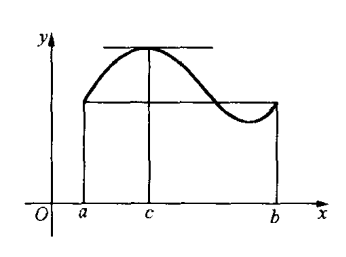
\includegraphics[width=\textwidth]{3.1.png} % 无需重复指定宽度  
\end{myimagebox}     
\caption{\label{fig:3.1}第一型曲面积分的定义}   
\end{figure}

分割取极限不难得到,这个极限可以写作:

\begin{align*}
\iint_S \rho(x;y;z)\mathrm{d}S\tag{3-1}  
\end{align*}

注意这里的$S$是曲面面积。如图3.1所示。

第一型曲面积分与第一型曲线积分类似,具有可加性,区域可合并性,并且是\textbf{\color{brown!50!red}无方向的}。

第一型曲面积分也可以计算曲面的面积,只需要令$\rho(x;y;z)=1$即可,这也因此和我们在重积分的应用里面所提到的一致。

\subsubsection{第一型曲面积分的计算}
对于第一型曲面积分的计算主要是对于$\mathrm{d}S$的处理。这里处理方式如式子1-21,1-22,1-23所示。我们这里直接给出一道例题,通过两种方法计算,帮助读者更好了解第一型曲面积分的计算方法。

\textbf{例}:设曲面$S$是$z=\sqrt{x^2+y^2}$被$x^2+y^2=2ax$割下的部分。求第一型曲面积分:
\begin{align*}
    I=\iint_S(x^2y^2+y^2z^2+z^2x^2)\mathrm{d}S
\end{align*}

\textbf{解}:第一种方法是在直角坐标系下计算:
\begin{align*}
    \frac{\partial z}{\partial x}=\frac{x}{\sqrt{x^2+y^2}}\qquad \frac{\partial z}{\partial y}=\frac{y}{\sqrt{x^2+y^2}}\qquad \sqrt{1+z_x^2+z_y^2}=\sqrt{2}
\end{align*}

因此原积分转化为:
\begin{align*}
I=\iint_D[x^2y^2(x^2+y^2)^2]\cdot\sqrt{2}\mathrm{d}x\mathrm{d}y
\end{align*}

其中$D:x^2+y^2\leq 2ax$。用极坐标换元$x=r\cos\theta,y=r\sin\theta$:
\begin{align*}
I&=\sqrt{2}\int_{-\pi/2}^{\pi/2}\mathrm{d}\theta\int_0^{2a\cos\theta}(r^4\cos^2\theta\sin^2\theta+r^4)r\mathrm{d}r\\
&=  \sqrt{2}\int_{-\pi/2}^{\pi/2}(\cos^2\theta\sin^2\theta+1)(\left.\frac{1}{6}r^6\right|_0^{2a\cos\theta})\mathrm{d}\theta\\
&=\frac{\sqrt{2}}{6}(2a)^6\int_{-\pi/2}^{\pi/2}(\cos^2\theta\sin^2\theta+1)\cos^6\theta\mathrm{d}\theta\\
&=\frac{64\sqrt{2}}{3}a^6\int_0^{\pi/2}(\cos^8\theta-\cos^{10}\theta+\cos^6\theta)\mathrm{d}\theta\\
&=\frac{64\sqrt{2}}{3}a^6\times\frac{\pi}{2}\times(\frac{35}{128}-\frac{63}{256}+\frac{5}{16})\\
&=\frac{29\sqrt{2}}{8}\pi a^6
\end{align*}

第二种办法采用球坐标换元。根据$z=\sqrt{x^2+y^2}$可得,球坐标参数$\varphi=\frac{\pi}{4}$。因此令$x=\frac{r\cos\theta}{\sqrt{2}},y=\frac{r\sin\theta}{\sqrt{2}},z=\frac{r}{\sqrt{2}}$。那么由于曲面的边界为$x^2+y^2=2ax$,因此得到:
\begin{align*}
    D=\{(r,\theta)| \theta\in[-\frac{\pi}{2},\frac{\pi}{2}],r\in[0,2\sqrt{2}a\cos\theta]\}
\end{align*}

因此解得$E=\frac{1}{2}r^2,F=0,G=1$,积分化简为:
\begin{align*}
    I&=\int_{-\pi/2}^{\pi/2}\mathrm{d}\theta\int_0^{2\sqrt{2}a\cos\theta}(\frac{1}{4}r^4\cos^2\theta\sin^2\theta+\frac{1}{4}r^4)\frac{r}{\sqrt{2}}\mathrm{d}r\\
    &=\frac{29\sqrt{2}}{8}\pi a^6
\end{align*}
\subsection{第二型曲面积分}
\subsubsection{第二型曲面积分的定义}
类似于第二型曲线积分一样我们先引入一些定义。我们先介绍什么是\textbf{\color{brown!50!red}双侧正则曲面}。定义一个在三维空间的曲面$S$,且曲面上任意一点$P$处可以定义两个法方向的单位法向量$\bm{n}^+,\bm{n}^-$。当点$P$运动时,这两个法向量也会连续运动。当点$P$在曲面上又运动回到起点时,这两个法向量的方向不变。就说$S$是双侧正则曲面。显然我们可以发现,莫比乌斯环不是一个双侧正则曲面。

双侧正则曲面的正面和背面如何证明?在重积分的应用得点P处的法向量$(f_x,f_y,-1)$与$(-f_x,-f_y,1)$。如果选定第一个法向量为参与积分的法向量,则定义是\textbf{\color{brown!50!red}曲面的正侧}。反之为反侧。

第二型曲面积分的物理背景是什么?假设有一个河道,并且河道里中的水的流速由下边的矢量函数给出:$\bm{v}=(P(x;y;z),Q(x;y;z),R(x;y;z))$,定义河道里一个双侧曲面并且选定一侧,问单位时间流出这个面的水的流量。

显然每一个面积微元$S_i$的流量为$\bm{v_i}\cdot \bm{n_i}$,因此定义第二型曲面积分为:
\begin{align*}
\iint_S \bm{f} (P;Q;R)\cdot \bm{n}(P;Q;R) \mathrm{d}S = 
\iint_S \bm{f} (P;Q;R)\cdot  \mathrm{d}\bm{S}\tag{3-2} 
\end{align*}

第二型曲面积分是有方向的,因此取不同的面积分,得到的结果是相反的。

第二型曲面积分该如何表示?我们看3.2左侧,这是一个向量点乘,而法向量可以由方向余弦$(\cos\alpha,\cos\beta,\cos\gamma)$表示。

\begin{tcolorbox}[
    colback=bac2,     % 极浅黄色背景
    colframe=fra2,   % 浅黄色边框
    coltitle=white,             % 标题文字白色
    coltext=tex2,
    title=第二型曲面积分的表示,
    fonttitle=\bfseries,        % 标题加粗
arc=3mm,                     % 圆角稍大
breakable
]
根据上式,积分可以表示为:
\begin{align*}
I=\iint_SP(x;y;z)\cos\alpha+Q(x;y;z)\cos\beta+R(x;y;z)\cos\gamma\mathrm{d}S \tag{3-3} 
\end{align*}

3-3表示了第一型曲面积分和第二型曲面积分之间的关系。在法向量的坐标好求的时候,我们可以直接转化成第一型曲面积分进行计算(这也是第二型曲面积分的方向角表示法)。

接下来我们来观察$\cos\gamma\mathrm{d}S$的含义。如图3.2所示。与$z$轴的方向余弦与曲面面积微元的乘积就是其曲面在$Oxy$的投影面积微元。因此我们可以得到:
\begin{align*}
I=\iint_{S}P(x;y;z)\mathrm
{d}y\mathrm{d}z+Q(x;y;z)\mathrm
{d}z\mathrm{d}x+R(x;y;z)\mathrm
{d}x\mathrm{d}y \tag{3-4} 
\end{align*}

\begin{figure}[H]    
\centering     
\renewcommand{\figurename}{图}     
\renewcommand{\thefigure}{3.2}    
\begin{myimagebox}[width=0.35\textwidth] % 直接传入图片尺寸参数      
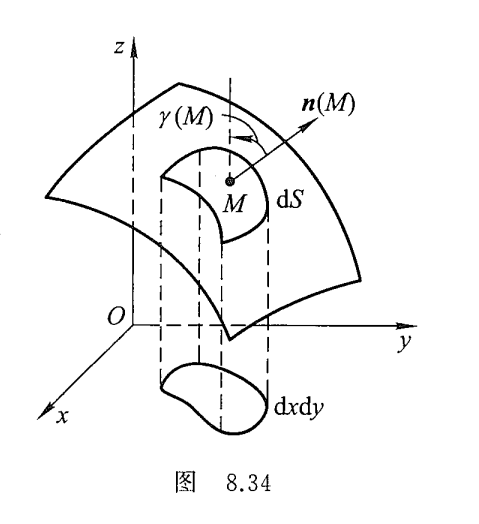
\includegraphics[width=\textwidth]{3.2.png} % 无需重复指定宽度  
\end{myimagebox}     
\caption{\label{fig:3.2}第一型曲面积分的定义}   
\end{figure}

\end{tcolorbox}


\textbf{\color{brown!50!red}然而这和重积分有很大区别}。一方面,积分区域是一个三维曲面,因此你不能直接去把它看作是三个二重积分的和;另一方面,积分函数是三元函数。还有一个问题就是,这里的$\mathrm{d}x\mathrm{d}y$等\textbf{\color{brown!50!red}微元是有正负号的,因为它受到了方向余弦的正负控制}。

\subsubsection{第二型曲面积分的计算}
第二型曲面积分计算的第一步是\textbf{\color{brown!50!red}转化成第一型曲面积分}。在一些特殊的例子中可以一步计算。

\textbf{\color{brown!50!red}例}:令积分区域为$x^2+y^2+z^2=R^2$的外侧,计算积分:
\begin{align*}
I=\iint_S\frac{(x,y,z)}{\sqrt{x^2+y^2+z^2}}\cdot \bm{n}^+  \mathrm{d}S 
\end{align*}

\textbf{\color{brown!50!red}解}:这里直接求方向余弦即可。
\begin{align*}
I&=\iint_S\frac{(x,y,z)}{\sqrt{x^2+y^2+z^2}}\cdot \frac{(x,y,z)}{\sqrt{x^2+y^2+z^2}}  \mathrm{d}S 
\\&=\iint_S\frac{1}{x^2+y^2+z^2}\mathrm{d}S\\
&=\frac{1}{r^2}\iint_S\mathrm{d}S=4\pi   
\end{align*}


计算第二型曲面积分的第二步是转化成\textbf{\color{brown!50!red}二重积分}。假设曲面的表达式为$z=f(x;y)$。我们先看第二型曲面积分的定义式3-2,假设在曲面正侧积分,那么法向量的表达式为:
\begin{align*}
\bm{n}^+ =\frac{(-f_x,-f_y,1)}{\sqrt{f_x^2+f_y^2+1}}  
\end{align*}

同时$\mathrm{d}S=\sqrt{1+f_x^2+f_y^2}\mathrm{d}\sigma$代入到3-3进行计算:
\begin{align*}
I&=\iint_\sigma (-Pf_x-Qf_y+R )\frac{1}{\sqrt{f_x^2+f_y^2+1} } \cdot(f_x^2+f_y^2+1)\mathrm{d}\sigma\\
&= \iint_\sigma (-Pf_x-Qf_y+R )\mathrm{d}\sigma\tag{3-5} 
\end{align*}

其中$\sigma$为曲面在$Oxy$的投影。

\textbf{\color{brown!50!red}例}:已知S是球面$z=\sqrt{R^2-x^2-y^2}$的上侧,计算积分:
\begin{align*}
    I=\iint_S yz\mathrm{d}z\mathrm{d}x+zx\mathrm{d}x\mathrm{d}y
\end{align*}

\textbf{\color{brown!50!red}解}:注意到这里$P=0,Q=yz.R=zx,-f_y=\frac{y}{z}$,因此直接带入:
\begin{align*}
 I&=\iint_D (yz\times\frac{y}{z}+zx)\mathrm{d}\sigma \\
&=\iint_D  y^2+x\sqrt{R^2-x^2-y^2}\mathrm{d}x\mathrm{d}y\\
&= \int_0^{2\pi}\mathrm{d}\theta\int_0^R(r^2\sin^2\theta+r\cos\theta\sqrt{R^2-r^2})r\mathrm{d}r
\\&=\int_0^{2\pi}\frac{R^4}{4}\sin^2\theta+\frac{1}{16}R^4\cos\theta\mathrm{d}\theta\\ 
&=\frac{1}{4} \pi R^4
\end{align*}

当曲面被参数化的时候,即$x=x(u,v),y=y(u,v),z=z(u,v)$,法向量是$(A,B,C)$,投影面积是$\sqrt{A^2+B^2+C^2}\mathrm{d}\sigma$,二重积分可以表示成:
\begin{align*}
I=\iint_{D_{uv}}(PA+QB+RC)\mathrm{d}\sigma_{uv}\tag{3-6}
\end{align*}

例:利用球坐标重新计算上一题。

解:令$x=R\sin\varphi\cos\theta,y=R\sin\varphi\sin\theta,z=R\cos\varphi$,则$A=R^2\sin^2\varphi\cos\theta,B=R^2\sin^2\varphi\sin\theta,C=R^2\sin\varphi\cos\varphi$,带入计算得:
\begin{align*}
 I&=\iint_D (R^2\sin\varphi\cos\varphi\sin\theta\times R^2\sin^2\varphi\sin\theta
+R^2\sin\varphi\cos\theta\cos\varphi\times R^2\sin\varphi\cos\varphi)\mathrm{d}\sigma \\
&=R^4\int_0^{2\pi}\mathrm{d}\theta\int_0^\frac{\pi}{2} 
(\sin^3\varphi\cos\varphi\sin^2\theta+\sin^2\varphi\cos^2\varphi\cos\theta)\mathrm{d}\varphi
\\&=R^4\int_0^{2\pi}\frac{1}{4}\sin^2\theta+\frac{1}{16}\cos\theta\mathrm{d}\theta\\ 
&=\frac{1}{4} \pi R^4
\end{align*}

\subsection{高斯公式与斯托克斯公式}
\subsubsection{高斯公式}
在格林公式的延伸中,我们根据2.11得到了一个结论。在这里我们令$P_x+Q_y$是向量$\bm{F}$的\textbf{\color{brown!50!red}散度},拓展到三维空间的向量散度表示为:
\begin{align*}
    \nabla\cdot F=(\frac{\partial}{\partial x},\frac{\partial}{\partial y},
\frac{\partial}{\partial z})\cdot(P,Q,R)=P_x+Q_y+R_z
\end{align*}

因此我们在2.11得到了$\oint_c \bm{F}\cdot \bm{n}\mathrm{d}s=\iint_D\nabla\cdot\bm{F}\mathrm{d}\sigma$。把这个结论拓展到三维空间就得到了\textbf{\color{brown!50!red}Gauss公式}:

\begin{tcolorbox}[
    colback=bac2,     % 极浅黄色背景
    colframe=fra2,   % 浅黄色边框
    coltitle=white,             % 标题文字白色
    coltext=tex2,
    title=Gauss公式,
    fonttitle=\bfseries,        % 标题加粗
arc=3mm,                     % 圆角稍大
breakable
]
设$\Omega$为三维区域有界区域,其边界是若干分片光滑曲面$S$,$F=(P,Q,R)\in C^1$,且积分面在\textbf{\color{brown!50!red}外侧},则:
\begin{align*}
   \oiint_S \bm{F}\cdot \bm{n}\mathrm{d}s=\iiint_\Omega\nabla\cdot\bm{F}\mathrm{d}V\tag{3-7} 
\end{align*}
\end{tcolorbox}

证明方式与格林公式类似,取特殊区域$\Omega:\{(x,y)\in D_y,z\in[A(x,y),B(x,y)]\}$,则在这个空间有上底面,下底面,侧面$S_1,S_2,S_3$,单位法向量分别向上,向下,向外。则此时:
\begin{align*}
   \oiint_S R\mathrm{d}x\mathrm{d}y&=\iint_{S_1}R\mathrm{d}x\mathrm{d}y+\iint_{S_2}R\mathrm{d}x\mathrm{d}y\\
&=\iint_D R(x,y,A)\mathrm{d}\sigma-\iint_D R(x,y,B)\mathrm{d}\sigma\\
&=\iint_D\mathrm{d}\sigma\int_B^A\frac{\partial R}{\partial z}\mathrm{d}z\\
&=\iiint_\Omega R_z\mathrm{d}V 
\end{align*}

然后一般空间切割成这种曲面即可。

\textbf{\color{brown!50!red}例}:S是锥面$z=\sqrt{x^2+y^2},z\in[0,1]$的下侧,计算积分:
\begin{align*} 
  \iint_S (y-z)\mathrm{d}y\mathrm{d}z+(z-x)\mathrm{d}z\mathrm{d}x+(x-y^2)\mathrm{d}z\mathrm{d}y      
\end{align*}

\textbf{\color{brown!50!red}解}:我们\textbf{\color{brown!50!red}加一个盖子}$z=1$的圆,取上侧且在这个面上的积分为$I_1$,在整个表面上的积分为$I_2$,则:
\begin{align*} 
  I&=I_2-I_1=\iiint P_x+Q_y+R_z \mathrm{d}V-\iint_D (x-y^2)\mathrm{d}\sigma\\
&=\iint_{x^2+y^2\leq 1}(x-y^2)\mathrm{d}x\mathrm{d}y \\
&=\frac{-\pi}{4} 
\end{align*}

\textbf{\color{brown!50!red}例}:设曲面$S:x^2+y^2+z^2=1.a,b,c>0$,取外侧,计算积分:
\begin{align*} I=\iint_S\frac{x\mathrm{d}y\mathrm{d}z+y\mathrm{d}z\mathrm{d}x+z\mathrm{d}x\mathrm{d}y}
{(ax^2+by^2+cz^2)^{3/2}} 
\end{align*}

和格林公式的用法一样,我们要先观察$P,Q,R$有没有\textbf{\color{brown!50!red}一阶连续偏导}。显然在没有有原点的地方,满足$P_x+Q_y+R_z=0$,因此在没有原点的地方积分为0。

在有原点的地方,我们做曲面$S_\varepsilon:ax^2+by^2+cz^2=\varepsilon^2$,因此:
\begin{align*} 
  I&=\frac{1}{\varepsilon ^2} 
\iint_Sx\mathrm{d}y\mathrm{d}z+y\mathrm{d}z\mathrm{d}x+z\mathrm{d}x\mathrm{d}y\\
&=\frac{1}{\varepsilon ^2} \iiint1\mathrm{d}V=\frac{4\pi}{\sqrt{abc} } 
\end{align*}
\subsubsection{高斯公式的应用}
利用高斯公式可以用第二型曲面积分表示三维空间体体积。
\begin{tcolorbox}[
    colback=bac1,     % 极浅黄色背景
    colframe=fra1,   % 浅黄色边框
    coltitle=white,             % 标题文字白色
    coltext=tex1,
    title=三维空间体的体积,
    fonttitle=\bfseries,        % 标题加粗
arc=3mm,                     % 圆角稍大
breakable
]
三维空间体的体积可以表示为:
\begin{align*} 
  V&=\iiint_V1\mathrm{d}V=\oiint_S x\mathrm{d}y\mathrm{d}z  \\
&=\frac{1}{3}\oiint_Sx\mathrm{d}y\mathrm{d}z+y\mathrm{d}z\mathrm{d}x+z\mathrm{d}x\mathrm{d}y       \tag{3-8}
\end{align*}
\end{tcolorbox}

当空间表面方程参数化时$x=x(u,v),y=y(u,v),z=z(u,v)$,根据两种曲面积分的关系:
\begin{align*} 
  V
&=\frac{1}{3}\left|\oiint_S Ax+By+Cz\mathrm{d}u
\mathrm{d}v\right|\\
&=\frac{1}{3}\left|\begin{vmatrix}
 x & y & z\\
 x_u & y_u& z_u\\
 x_v & y_v &z_v
\end{vmatrix}  \mathrm{d}u\mathrm{d}v \right|\tag{3-9}      
\end{align*}

\subsubsection{斯托克斯公式}
在格林公式中,我们说明了$\oint_L \bm{F}\mathrm{d}\bm{r}=\iint_D(Q_y-P_x)\mathrm{d}\sigma$,如果把它扩展到三维情况呢?就是\textbf{\color{brown!50!red}Stokes公式}:
\begin{tcolorbox}[
    colback=bac1,     % 极浅黄色背景
    colframe=fra1,   % 浅黄色边框
    coltitle=white,             % 标题文字白色
    coltext=tex1,
    title=Stokes公式,
    fonttitle=\bfseries,        % 标题加粗
arc=3mm,                     % 圆角稍大
breakable
]
令$S$是三维空间中分片光滑双侧曲面,边界$\Gamma$是若干Jordan曲线,$S$的定向面上的法向量与边界方向\textbf{\color{brown!50!red}构成右手系},则:
\begin{align*} 
 \oint_L\bm{F}\mathrm{d}\bm{r}&=\iint_S(R_y-Q_z)\mathrm{d}y\mathrm{d}z+(P_z-R_x)\mathrm{d}z\mathrm
{d}x+(Q_x-P_y)\mathrm{d}x\mathrm{d}y \\
&=\iint_S\begin{vmatrix}
\mathrm{d}y\mathrm{d}z  & \mathrm{d}z\mathrm{d}x& \mathrm{d}x\mathrm{d}y\\
\frac{\partial}{\partial x}  & \frac{\partial}{\partial y} & \frac{\partial}{\partial z}\\
P  & Q & R
\end{vmatrix} \\ 
&=\iint_S \nabla\times\bm{F}\cdot \bm{n}\mathrm{d}S\tag{3-10}       
\end{align*}

其中$\nabla\times\bm{F}$称作\textbf{\color{brown!50!red}旋度},又称rot$\bm{F}$,其表示为:
\begin{align*} 
 \nabla \times \mathbf{F} = \begin{vmatrix}
\mathbf{i} & \mathbf{j} & \mathbf{k} \\
\frac{\partial}{\partial x} & \frac{\partial}{\partial y} & \frac{\partial}{\partial z} \\
F_x & F_y & F_z
\end{vmatrix} \tag{3-11}       
\end{align*}
\end{tcolorbox}

证明过程与高斯定理和格林公式类似,只需证明$\oint_LP\mathrm{d}x=\iint_S P_z\mathrm{d}z\mathrm{d}x-P_y\mathrm{d}x\mathrm{d}y$即可。我们将曲线参数化,令$x=x(u,v);y=y(u,v);z=z(u;v)$,则:
\begin{align*} 
 \oint_LP\mathrm{d}x&=\oint _\Gamma P(x;y;z)(x_u\mathrm{d}u+x_v\mathrm{d}v)\\
&=\oint_\Gamma (Px_u)\mathrm{d}u+(Px_v)\mathrm{d}v\\
&=\iint_S[(Px_v)_u-(Px_u)_v\mathrm{d}\sigma] \\
&=\iint_S(P_ux_v+Px_{uv}-P_vx_u-Px_{uv})\mathrm{d}\sigma   \\
&=\iint_S(P_xx_u+P_yy_u+P_zz_u)x_v-(P_xx_v+P_yy_v+P_zz_v)x_u\mathrm{d}\sigma\\ 
&=\iint_S-P_y(-y_ux_v+y_vx_u)+P_z(z_ux_v-z_vx_u)\mathrm{d}\sigma \\
&=\iint(-P_yC+P_zB)\mathrm{d}\sigma     
\end{align*}

\textbf{\color{brown!50!red}例}:已知$C$是立方体$\{(x,y,z)|0\leq x\leq a,0\leq y\leq a,0\leq z\leq a\}$的表面与平面$x+y+z=\frac{3a}{2}$的交线,取向是从$z$轴正向看的逆时针方向。计算:
\begin{align*} 
 I=\oint_C(y^2-z^2)\mathrm{d}x+(z^2-x^2)\mathrm{d}y+(x^2-y^2)\mathrm{d}z     
\end{align*}

\textbf{\color{brown!50!red}解}:如果不用Stokes公式,需要分六段计算,虽然有点麻烦,不过表示出来很简单。用Stokes公式,对于3-10我们利用两种积分关系,把行列式第一行写成方向向量,后面加上$\mathrm{d}S$,则解出:
\begin{align*} 
 I&=\iint_\sigma \begin{vmatrix}
 \frac{\sqrt{3} }{3}  & \frac{\sqrt{3} }{3} & \frac{\sqrt{3} }{3}\\
\frac{\partial }{\partial  x}  & \frac{\partial }{\partial  y}  & \frac{\partial }{\partial  z}\\
y^2-z^2  & z^2-x^2 &x^2-y^2
\end{vmatrix}   \mathrm{d}S \\
&=\frac{\sqrt{3} }{3}\iint_\sigma -4(x+y+z)\mathrm{d}S\\
&=-2\sqrt{3}aS_\sigma\\
&=\frac{-9a^3}{2}   
\end{align*}
\subsection{习题补充与扩展}
\textbf{\color{brown!50!red}例1}:求第一型曲面积分$F(t)=\iint_{x^2+y^2+z^2=t^2}f(x;y;z)\mathrm{d}S$,其中:
\begin{align*}
    f(x;y;z)=\begin{cases}
         x^2+y^2 & z\geq\sqrt{x^2+y^2}\\
         0 & z\leq\sqrt{x^2+y^2}
    \end{cases}
\end{align*}

\textbf{\color{brown!50!red}解}:根据题目条件,计算:
\begin{align*} 
  \sqrt{1+z_x^2+z_y^2}=\frac{|t|}{\sqrt{t^2-x^2-y^2}}  
\end{align*}

联立$x^2+y^2+z^2=t^2,z=\sqrt{x^2+y^2}$,得到$x^2+y^2=\frac{t^2}{2}$。因此:
\begin{align*} 
 I&=\iint_{x^2+y^2\leq t^2/2}(x^2+y^2)\frac{|t|}{\sqrt{t^2-(x^2+y^2)} }\mathrm{d}\sigma\\
&=|t|\int_0^{2\pi}\mathrm{d}\theta\int_0^{\frac{|t|}{\sqrt{2}}}\frac{r^3\mathrm{d}r }{\sqrt{t^2-r^2}} \\
&=\frac{(8-5\sqrt{2})\pi}{6} t^4 
\end{align*}

\textbf{\color{brown!50!red}例2}:已知$S: y^2+z^2=1$被$x=0,x=1,z+y=0,z-y=0$截取的上方部分,取外侧。计算积分:
\begin{align*} 
 I=\iint_Sx(z^2-y^2)\mathrm{d}y\mathrm{d}z+y(x^2-z^2)\mathrm{d}z\mathrm{d}x+  
 z(y^2-x^2)\mathrm{d}x\mathrm{d}y
\end{align*}

\textbf{\color{brown!50!red}解}:画出这个区域,然后换元$x=x,y=\sin\theta,z=\cos\theta$,则$x\in[0,1],\theta\in[\frac{-\pi}{4},\frac{\pi}{4}]$,然后计算参数:$A=0,B=\sin\theta,C=\cos\theta$。因此:
\begin{align*} 
 I=\int_{-\frac{\pi}{4} }^ \frac{\pi}{4}\mathrm{d}\theta\int_0^1x^2(\sin^2\theta-\cos^2\theta)
\mathrm{d}\theta =\frac{1}{3}   
\end{align*}

\textbf{\color{brown!50!red}例3}:已知$C:x=y,z=\sqrt{a^2-x^2-y^2}$交线,从$A(\frac{a}{\sqrt{2}},\frac{a}{\sqrt{2}},0)$到$B(-\frac{a}{\sqrt{2}},-\frac{a}{\sqrt{2}},0)$,求:
\begin{align*} 
 I=\int_C (z^3+3x^2y)\mathrm{d}x+(x^3+3y^2z)\mathrm{d}y+(y^3+3z^2x)\mathrm{d}z   
\end{align*}

\textbf{\color{brown!50!red}解}:连接AB,记作$\Gamma$,方向从B到A。则根据Stokes公式:
\begin{align*} 
 I_{C+\Gamma}&=\iint_S\begin{vmatrix}
 \mathrm{d}y\mathrm{d}z   & \mathrm{d}z\mathrm{d}x & \mathrm{d}x\mathrm{d}y\\
F_x  & F_y & F_z\\
z^3+3x^2y  & x^3+3y^2z &y^3+3z^2x
\end{vmatrix}=0\\
I&=\int_{-\Gamma}(z^3+3x^2y)\mathrm{d}x+(x^3+3y^2z)\mathrm{d}y+(y^3+3z^2x)\mathrm{d}z  \\
&=\int_{-a/\sqrt{2} }^{a/\sqrt{2} }(3t^3+t^3+t^3)\mathrm{d}t=0
\end{align*}

\textbf{\color{brown!50!red}例4}:设$\Gamma$是光滑闭曲面,围成的区域是$\Omega$,,$\bm{n}$是$\Gamma$上的单位外法向量,$(x_0,y_0,z_0)$是$\Omega$内固定一点,且$(x,y,z)\in\Gamma,\bm{r}=(x-x_0,y-y_0,z-z_0)$,试证明:
\begin{align*} 
\oiint_\Gamma\cos(\bm{n},\bm{r})\mathrm{d}S=2\iiint_\Omega\frac{\mathrm{d}x\mathrm{d}y\mathrm{d}z}
{|\bm{r}|}  
\end{align*}

\textbf{\color{brown!50!red}证明}:我们先令法向量的方向余弦$\cos \alpha,\cos\beta,\cos\gamma$,则:
\begin{align*} 
\cos(\bm{n},\bm{r})&=\cos(x,\bm{r})\cos\alpha+\cos(y,\bm{r})\cos\beta+\cos(z,\bm{r})\cos\gamma
\\&=\frac{x-x_0}{|\bm{r}|}\cos\alpha+\frac{y-y_0}{|\bm{r}|}\cos\beta+
\frac{z-z_0}{|\bm{r}|}\cos\gamma
\end{align*}

如果直接用高斯公式,由于在点$x_0,y_0,z_0$处的$P,Q,R$没有一节连续偏导,因此需要先挖一个球,不含此点用高斯定理:
\begin{align*} 
I&=\iiint_{\Omega_0}(\frac{x-x_0}{|\bm{r}|})_x+(\frac{y-y_0}{|\bm{r}|})_y+
(\frac{z-z_0}{|\bm{r}|})_z\mathrm{d}V\\
&=2\iiint_{\Omega_0}\frac{\mathrm{d}V }{|\bm{r}|} 
\end{align*}

而在这个球面上,由于$\bm{r}$与$\bm{n}$方向相反,即就$\cos(\bm{n},\bm{r})=-1$,因此$I=-4\pi\varepsilon^2\to 0$,证毕。

\section{常微分方程(ODE)}
\subsection{简论}
\subsubsection{基本定义}
定义一个联系自变量$x$,因变量$y$以及$n$阶导数的方程:
\begin{align*} 
  F(x,y^{(1)},y^{(2)},...,y^{(n)})=0\tag{4-1}
\end{align*}

称作\textbf{$n$阶ODE方程}。如果$y=y(x)$在区域$[a,b]$上满足4-1,则称$y(x)$为4-1的一个解。定义若函数集合$\psi(x,c_1,c_2,...,c_n)$都是4-1的解,其中$c_1,c_2,...c_n$都是独立常数,则称其为通解。通解中独立常数的个数就是ODE方程的阶数。

如果说带着$n$个参数的函数集合$\psi(x,c_1,c_2,...,c_n)$,这$n$个参数相互独立,则雅可比矩阵不应该为0,即就是:
\begin{align*} 
  \frac{D(\psi,\psi^{(1)},...,\psi^{(n-1)})}{D(c_1,c_2,..c_n)}\neq0\tag{4-2}
\end{align*}

\textbf{特解}指的是当这$n$个参数取特定值产生的某一个解。奇解是不包含在通解内的特解。如果一个函数$y(x)$不再通解内,但在任意点$x$处,$y(x)$与某一个通解相切,称$y(x)$为包络。特别的,包络是一阶ODE的奇解。例如方程$x+yy'=0$,必然有一个解$x^2+y^2=C$,这个就是奇解

\textbf{初值问题}就是找到4-1的一个解,$y=y(x),x\in[0,x]$,如果满足:
\begin{align*}
    y(0)=y_0\qquad y'(0)=y_1\quad...\quad y^{(n-1)}(0)=y_{n-1}
\end{align*}

那么这个问题就是初值问题。
\subsubsection{一阶ODE解的存在唯一性}
对于一阶ODE初值问题$y'=f(x;y),y(x_0)=y_0$是否有解,解是否唯一呢?我们先介绍Lipschitz性质:若$\exists L>0,\forall (x,y_1),(x,y_2)$,如果有:
\begin{align*} 
  |f(x;y_1)-f(x;y_2)|\leq L|y_1,y_2|\tag{4-3}
\end{align*}

则称$f(x;y)$在区域D上有关于$y$的Lipschitz连续。这就意味着如果$f_y$存在并且有界,则函数关于$y$的Lipschitz连续可以根据拉格朗日中值定理写作:
\begin{align*} 
  |f(x;y_1)-f(x;y_2)|=|f_y(x;\varepsilon )(y_2-y_1)|\leq L|y_1,y_2|
\end{align*}

接下来我们再介绍一个定理:设区域$D$是矩形$[x_0-a,x_0+a]\times[y_0-b,y_0+b]$,设函数$f(x;y)$在区域内有界,$\max|f(x;y)|=M$,且$f(X;y)$在区域D上有关于$y$的Lipschitz连续,则初值问题在区间$[x_0-h,x_0+h]$内有唯一解,其中$h=\min\{a,\frac{b}{M}\}$
\begin{figure}[h]
\centering
\renewcommand{\figurename}{图}
\renewcommand{\thefigure}{4.1}
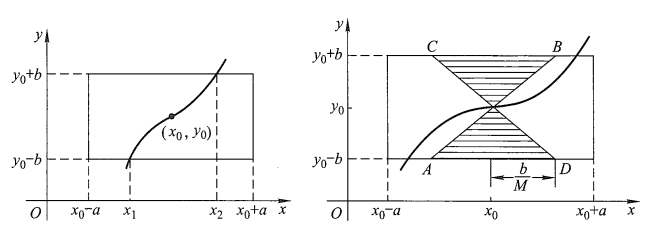
\includegraphics[width=0.69\textwidth]{4.1.png}
\caption{\label{fig:4.1.png}定理证明}
\end{figure}

我们先去理解定义讲了一个什么内容。在这张图虽然$f(x;y)$在区域有定义,然而原函数可能如右侧的方式穿过区域D,当这种情况发生时,$x<x_1;x>x_2$的两部分原函数超过了区域,$f(x;y)$没有定义。如果$|f|\leq M$,则原函数斜率绝对值不会大于$M$。我们过$(x_0,y_0)$做两条斜率为$M$的曲线,那么函数$f(x;y)$会被严格限制在矩形$ABCD$内侧,那么$x_D-x_0=\min\{a,\frac{b}{M}\}$。接下来我们来证明这个定理。

第一步是\textbf{\color{brown!50!red}构造Picard序列}:我们首先指出一阶初值问题与积分方程:
\begin{align*} 
  y=y_0+\int_{x_0}^x f(x;y)\mathrm{d}x \tag{4-4}
\end{align*}

是等价的(这个很好证明)。首先将常数函数$y(x)=y(0),x\in[x_0-h,x_0+h]$带到积分方程进行拟合,得到一阶近似解:
\begin{align*} 
  y_1(x)=y_0+\int_{x_0}^x f(x;y_0)\mathrm{d}x \tag{4-5}
\end{align*}

根据这个式子,我们得到:
\begin{align*} 
  |y_1(x)-y_0|=|\int_{x_0}^x f(x;y_0)\mathrm{d}x|\leq M|x-x_0|\leq b 
\end{align*}

因此$(x,y_1(x))$就在区域内。因此继续做二阶近似解:
\begin{align*} 
  y_2(x)=y_0+\int_{x_0}^x f(x;y_1(x))\mathrm{d}x 
\end{align*}

同理可以证明,$(x,y_2(x))$也在区域内。因此我们可以做到$n$阶近似。其中$x\in[x_0-h,x_0+h]$。上述近似解$y_1(x),y_2(x)...y_n(x)$为Picard序列。

第二步:证明$n\to\infty$的时候皮卡序列的极限函数存在,即就是:
\begin{align*} 
  \lim_{n\to\infty}y_n(x)=\varphi(x)\qquad x\in[x_0-h,x_0+h]
\end{align*}

第三步:对原积分函数同时求极限,就是:
\begin{align*} \varphi(x)=y_0+\int_{x_0}^{x}f(x;\varphi(x))\mathrm{d}x \qquad x\in[x_0-h,x_0+h]\tag{a}
\end{align*}

接下来去证明解是唯一的。假设我们存在另一个解$\psi(x)$,只需要证明与$\varphi(x)$等价即可。并注意函数满足Lipschitz连续,则有:
\begin{align*}
|\psi(x)-\varphi(x)|&\leq L|\int _{x_0}^x|\varphi(x)-\psi(x) |\mathrm{d}x |\\
&\leq LA|x-x_0|
\end{align*}

把这个式子代入a式,得到:
\begin{align*}
|\psi(x)-\varphi(x)|&\leq A\frac{(L|x-x_0|)^2}{2!}
\end{align*}

反复带回到式子a,得到:
\begin{align*}
|\psi(x)-\varphi(x)|&\leq A\frac{(L|x-x_0|)^n}{n!}\leq \lim_{n\to\infty}A\frac{(LA)^n}{n!}=0 
\end{align*}

证毕。在这一块我们主要需要掌握Picard序列的构造。我们来看一道例题:考虑初值问题$y'=x^2+y^2,y(0)=0$的Picard序列前三项。

\textbf{\color{brown!50!red}解}:我们先要把$y$转化成积分式:
\begin{align*}
y=\int_0^{x}(x^2+y^2)\mathrm{d}x 
\end{align*}

将$y=0$代入到积分式中,得到一阶Picard序列:
\begin{align*}
y_1=\int_0^{x}(x^2+0^2)\mathrm{d}x=\frac{1}{3}x^3  
\end{align*}

将$y=\frac{x^3}{3}$代入积分式得到二阶Picard序列:
\begin{align*}
y_1=\int_0^{x}(x^2+(\frac{1}{3}x ^3)^2)\mathrm{d}x=\frac{1}{3}x^3  +\frac{1}{63}x^7 
\end{align*}

三阶Picard序列同理。这里不再赘述。

\subsection{(一阶微分方程的)初等积分法}
一阶ODE一般利用不定积分去求解,即就是:
\begin{align*}
y'=f(x)\to y(x)=\int_0^xf(s)\mathrm{d}s+C  
\end{align*}

接下来的办法都是基于化成这种形式来计算的。注意:并非所有一阶ODE有初等函数解,我们能解出来的ODE实质上少之又少。
\subsubsection{变量分离方程}
变量分离的方程有下面的这种形式:
\begin{align*}
y'(x)=f(x)\cdot g(y) 
\end{align*}

不妨设$y(x),x\in[a,b],y\neq0$是一个解。如果$y>0$,那么就有:
\begin{align*}
\frac{y'(x)}{g(y)}=f(x)\to\frac{\mathrm{d}y }{g(y)}=f(x)\mathrm{d}x\to\ln|g(y)|=\int f(x)\mathrm{d}x  =F(x)+C   
\end{align*}

那么我们得到了$g(y)$的表达式,那么$y$的表达式能否直接求反函数,即$y=G^{-1}(F(x)+C)$是否存在。由于$G'(y)=g(y)^{-1}>0$,因此反函数存在。我们来判断参数是否独立,即就是:
\begin{align*}
\frac{\partial  y}{\partial C}=\frac{1}{G'(y)}> 0
\end{align*}

因此C是独立常数。并且如果再给出$g(y_0)=0$,那么$y(x)=y(0)$就是一个解。例:解ODE$y'=axy,a>0$,$y=y^{3/4}$

\textbf{\color{brown!50!red}解}:第一题对于上方的表达式我们可以计算出:
\begin{align*}
\frac{\mathrm{d}y}{y}=ax\mathrm{d}x\to \ln y=\frac{1}{2}ax^2+C\to y=Ce^{\frac{1}{2}ax^2 }  
\end{align*}

然而你要把$y$除过去,$y\neq 0$。我们再验证$y=0$时,原式也成立。因此$y=0$是一个\textbf{\color{brown!50!red}特解/奇解}。而根据上一章我们说,\textbf{\color{brown!50!red}特解是通解的包络}。这是因为:本质上$x=0$是所有通解形成的函数的渐进公切线。

第二问也是如此,$y=0$是一个特解,$y=(\frac{x+c}{4})^4$是通解,特解是通解的包络。

接下来我们看一些能化作变量分离的一阶ODE:第一种形式,$y'=f(ax+by+c)$,例题:解$y'=\sin(x+y+1)$。我们可以令$z=x+y+1$,那么$z'=1+y'=1+\sin z$,,因此:
\begin{align*}
\int\frac{\mathrm{d}z }{1+\sin z}=\int 1\mathrm{d}x\to \tan(\frac{z}{2}-\frac{\pi}{4} )=x+C
\end{align*}

积分这一步使用了万能公式。接下来我们看第二种形式:$y'=f(\frac{y}{x})$。因此我们可以换元$u=\frac{y}{x}$,则$y'=u'x+u$,即就是:
\begin{align*}
u'x+u=h(u)\to \int\frac{1}{x}\mathrm{d}x=\int\frac{\mathrm{d}u }{h(u)-u} \tag{4-6} 
\end{align*}

第三种形式是$y'=f(\frac{a_1x+b_1y+c_1}{a_2x+b_2y+c_2})$,这种形式比较复杂,我们先需要看下面的这个方程组:
\begin{align*}
\begin{cases}
a_1x+b_1y+c_1=0\\
a_2x+b_2y+c_2=0
\end{cases}      
\end{align*}

是否有解。根据Crammer法则,如果$a_1b_2-a_2b_1\neq0$,那么方程有唯一解$x_0,y_0$,因此:
\begin{align*}
y'=f\left(\frac{a_1(x-x_0)+b_1(y-y_0)}{a_2(x-x_0)+b_2(y-y_0)} \right)    
=f\left(\frac{a_1x^*+b_1y^*}{a_2x^*+b_2y^*} \right)
=f\left(\frac{a_1+b_1u}{a_2+b_2u} \right)\tag{4-7}
\end{align*}

如果$a_1b_2-a_2b_1=0$,那么就是存在常数$k$,使得$k(a_1,b_1)=(a_2,b_2)$。此时:
\begin{align*}
y'=f\left(\frac{a_1x+b_1y+C_1}{k(a_1x+b_1y)+C_2} \right)    
=f\left(\frac{u+C_1}{ku+C_2} \right)\tag{4-8}
\end{align*}

如果在上边的情况进一步,$a_1=b_1=0$,那么我们找不到常数$k$,但其实是退化到了$y'=f(ax+by+C)$类似的情况。我们看一道例题:解方程$y'=\frac{2x+y+1}{4x+2y-3}$。

这是我们上述说的第二种情况,因此令$2x+y+1=u$,则$u'=2+y'$,因此:
\begin{align*}
u'-2=\frac{u}{2u-5} \to \mathrm{d}u\frac{2u-5}{5u-10}=\mathrm{d}x \to\frac{2}{5}u-
\frac{1}{5}\ln (5u-10)=x+C   
\end{align*}

\subsubsection{一阶非齐次线性ODE}
再推而广之,一阶ODE的形式为:
\begin{align*}
    y'+P(x)y=Q(x)
\end{align*}

我们先前研究的是$Q(x)=0$的形式,称作齐次方程。而满足齐次条件线性方程则会有一个重要的性质:若$y_1,y_2$为解,则$C_1y_1+C_2y_2$也为解。然而在非齐次条件下,$Q(x)\neq 0$,那么此时该怎么去解呢?我们有两种办法:

第一种是常数变易法。我们假设$Q(x)=0$,那么我们可以解出:
\begin{align*}
    y=Ce^{f(x)}=Ce^{\int_{x_0}^xP(s)\mathrm{d}s}
\end{align*}

那么常数变易法就是假设这个常数是一个关于$x$的函数,即就是$C=u(x)$,因此:
\begin{align*}
   (ue^{-F})'+Pue^{-F}&=Q
\\u'e^{-F}&=Q\\
u&=\int_{x_0}^xQ(t)e^{F(t)}\mathrm{d}t+C 
\end{align*}

因此我们发现:\textbf{\color{brown!50!red}非齐次线性通解就是一个特解与齐次通解的组合}。

第二种情况不是通用的,即就是积分因子法。由于我们对$f(x;y)=0$做全微分可以得到:
\begin{align*}
    P(x;y)+Q(x;y)y'=0
\end{align*}

根据在Green公式一章,如果$P_y=Q_x$,那么就存在原函数$u$,把原式可以化作全微分方程。即就是$\mathrm{d}u=0$。

当然有的时候可能需要变形,例如同时乘一个函数或者除一个函数,对于一般地无法直接化成全微分方程的式子$M\mathrm{d}x+N\mathrm{d}y=0$,我们可以同乘一个函数$\mu$,使之存在原函数,即就是:
\begin{align*}
    \mu M\mathrm{d}x+\mu N\mathrm{d}y=0
\end{align*}

此时我们称$\mu$是\textbf{\color{brown!50!red}积分因子}。当然一般来说,我们可以假设积分因子只是$x$的函数或者只是$y$的函数,然后进行计算。

\textbf{\color{brown!50!red}例}:利用合适的办法求解如下微分方程:
\begin{align*}
    (2xy^2-y)\mathrm{d}x+(x+3y^3)\mathrm{d}y=0
\end{align*}

\textbf{\color{brown!50!red}解}:如果利用常数变易法,我们先把一阶ODE化作标准形式,即就是:
\begin{align*}
 y'+\frac{2xy^2-y}{x+3y^3}=0 
\end{align*}

我们发现化简不到常规形式,因此这个题我们考虑积分因子法。假设积分因子是关于$y$的函数,则:
\begin{align*}
 \frac{\partial [\mu(x+3y^3)]}{\partial x }&=\frac{\partial[\mu(2xy^2-y)]}{\partial y}\\
 \mu&=\mu_y(2xy^2-y)+\mu(4xy-1)\\
\mu&=\frac{1}{y^2}
\end{align*}

因此代入积分因子可以得到:
\begin{align*}
 P=&\mu M=2x-\frac{1}{y}\quad Q=\mu N=\frac{x}{y^2}+3y\\
u=&x^2+\frac{3}{2}y^2-\frac{x}{y}=C    
\end{align*}

\subsubsection{可降阶的二次方程}
有一些特殊的二阶方程可以化成一阶方程进行计算。第一种是不显式含$y$的式子,即$F=(x,y',y'')$,此时我们令$z=y'$即可。例如解方程$y''=a\sqrt{1+(y')^2}$

我们假设$z=y'$,原方程变为:
\begin{align*}
 z'=a\sqrt{1+z^2}\quad& \ln(z+\sqrt{1+z^2})=ax+C_1\\
&z=\sinh (ax+C_1)    
\end{align*}

第二种是不显示含$x$的情况,例如$F=(y,y',y'')$。我们假设$y'=P$,那么:
\begin{align*}
 \frac{\mathrm{d}P}{\mathrm{d}y }&=\frac{\mathrm{d}P}{\mathrm{d}x }\cdot  \frac{\mathrm{d}x}{\mathrm{d}y }\\
   y''&={y'}\frac{\mathrm{d}P}{\mathrm{d}y }
\end{align*}

例题:解初值问题:$1+(y')^2=2y'y'',y(1)=1,y'(1)=-1$。我们令$P=y'$,则$y''=y\frac{\mathrm{d}P}{\mathrm{d}y}$,带入到原式得到:
\begin{align*}
1+p^2&=2yp\frac{\mathrm{d}p}{\mathrm{d}y}\\
\frac{p\mathrm{d}p }{1+p^2}&=\frac{\mathrm{d}y }{2y}\\
1+p^2&=C_1|y|\\
  p&=-\sqrt{2y-1}\\
\sqrt{2y-1}&=2-x  
\end{align*}

这里注意一般是$\ln |y|$,而要注意的是,$y$在1附近的时候,$p$要在-1附近。

\subsection{二阶常系数线性ODE}
\subsubsection{齐次方程}
我们先看一个高阶线性常系数方程:
\begin{align*}
y^{(n)}+P_1y^{(n-1)}+...+P_{n-1}y'+P_ny=0\tag{4-9}   
\end{align*}

它的解的求法如下:先写出相应的特征多项式:
\begin{align*}
\lambda^n+P_1\lambda^{n-1}+...+P_{n-1}\lambda+P_n=0
\end{align*}

这个特征多项式是有很多解的。我们对于每一个解$\lambda$,如果$\lambda,\lambda^*$是共轭$k$重根,那么解的形式一定是下面函数的组合:
\begin{align*}
e^{\lambda x},e^{\lambda^*x},xe^{\lambda x},xe^{\lambda^*x},...,
x^{k-1}e^{\lambda x},x^{k-1}e^{\lambda^*x}\tag{4-10} 
\end{align*}

接下来我们来具体分析一些情况:第一种,当$\lambda$为实数根的时候,此时$\lambda=\lambda^*$,此时4-10化简为:
\begin{align*}
e^{\lambda x},xe^{\lambda x},...,
x^{k-1}e^{\lambda x}\tag{4-11} 
\end{align*}

特殊的,在二阶常系数中,根只可能是二重或者一重。一重的时候解为$e^{\lambda x}$。当$\lambda=a+bi$的时候,那么我们注意到:
\begin{align*}
e^{\lambda x}=e^{ax}(\cos bx+i\sin bx)\quad e^{\lambda^* x}=e^{ax}(\cos bx-i\sin bx)
\end{align*}

那么这两个函数本质上也是
\begin{align*}
e^{ax}\cos bx\quad e^{ax}\sin bx
\end{align*}

做线性变换得到的。因此4-10可以进一步化简成:
\begin{align*}
e^{ax}\cos bx,e^{ax}\sin bx,xe^{ax}\cos bx,xe^{ax}\sin bx,...\tag{4-12} 
\end{align*}

\textbf{\color{brown!50!red}例}:解方程$4y''-12y'+9y=0$。对于这个题解特征方程得出二重根$\lambda=\frac{3}{2}$,因此原方程通解为:
\begin{align*}
    y=C_1e^{\frac{3}{2}x}+C_2xe^{\frac{3}{2}x}
\end{align*}

\subsubsection{非齐次方程}
我们接下来讨论的是如下情况的非齐次方程:
\begin{align*}
    y''+py'+qy=f(x)\tag{4-13}
\end{align*}

首先它的通解在上一部分已经介绍。那么我们这一部分的主要内容是讨论其特解的形式。这一部分我们只介绍简单的形式。\textbf{\color{brown!50!red}第一种形式}为:
\begin{align*}
    f(x)=a_0x^n+a_1x^{n-1}+...+a_n(a_0\neq0)
\end{align*}

那么我们可以发现通解也是一个多项式,且通解$\psi$是由函数$Q(x)=b_0x^n+b_0x^{n-1}+...+b_n$变化而来的。接下来我们继续分类讨论:

\textbf{\color{brown!50!red}1.1}:当$p,q\neq0$时,此时$\psi=Q(x)$,利用待定系数法带回到原方程有:
\begin{align*}
\begin{cases}
qb_0=a_0\\
npb_0+qb_1=a_1\\
...
\end{cases} \tag{4-14}
\end{align*}

\textbf{\color{brown!50!red}1.2}:当$p\neq0,q=0$时,那么解的形式为:
\begin{align*}
    \psi=xQ(x)\tag{4-15}
\end{align*}

\textbf{\color{brown!50!red}1.3}:当$p=q=0$时,那么解的形式为:
\begin{align*}
    \psi=x^2Q(x)\tag{4-16}
\end{align*}

\textbf{\color{brown!50!red}第二种形式}为:
\begin{align*}
    f(x)=ae^{\alpha x},\alpha\in\mathbb{R},\alpha\neq0
\end{align*}

\textbf{\color{brown!50!red}2.1}:$\alpha$不是特征根($\alpha^2+p\alpha+q\neq0$),此时解的形式为:
\begin{gather*}
\psi=Ae^{\alpha x}\tag{4-17}\\
A\alpha^2e^{\alpha x}+Ap\alpha e^{\alpha x}+Aqe^{\alpha x}=ae^{\alpha x}\\
\psi=\frac{a}{\alpha^2+p\alpha+q}e^{\alpha x} 
\end{gather*}

\textbf{\color{brown!50!red}2.2}:$\alpha$是特征根且为单重根,那么解的形式为:
\begin{gather*}
\psi=Axe^{\alpha x}\tag{4-18}\\
\psi=\frac{a}{2\alpha+p}xe^{\alpha x} 
\end{gather*}

\textbf{\color{brown!50!red}2.3}:$\alpha$是特征根且是二重根,那么解的形式为:
\begin{gather*}
\psi=Ax^2e^{\alpha x}\tag{4-19}\\
\psi=\frac{a}{2}x^2e^{\alpha x} 
\end{gather*}

\textbf{\color{brown!50!red}第三种形式}为:
\begin{align*}
    f(x)=a\cos\beta x+b\cos\beta x
\end{align*}

\textbf{\color{brown!50!red}3.1}:$i\beta$不是原方程的一个根,此时解的形式为:
\begin{gather*}
  \psi=A\cos\beta x+B\sin\beta x\tag{4-20}\\
-A\beta^2\cos\beta x-B\beta^2\sin\beta x+p(-A\beta\sin\beta x+B\beta\cos\beta x)
+q(A\cos\beta x+B\sin\beta x)=f(x)\\
(q-\beta^2)A+p\beta b=a\quad -p\beta A+(q-\beta^2)B=b
\end{gather*}

\textbf{\color{brown!50!red}3.2}:$i\beta$是原方程的一个根,此时解的形式为:
\begin{align*}
    \psi=x(A\cos\beta x+B\sin\beta x)\tag{4-21}
\end{align*}

上面的几种情况可以总结为一般形式,对于$f(x)$形如:
\begin{gather*}
  f(x)=P_n(x)e^{\alpha x}(a\cos\beta x+b\sin\beta x)
\end{gather*}

\textbf{\color{brown!50!red}4.1}:如果$\alpha\pm i\beta$不是特征根,特解的形式为:
\begin{gather*}
  \psi=e^{\alpha x}(Q_n(x)\cos\beta x+R_n(x)\sin\beta x)\tag{4-22} 
\end{gather*}

\textbf{\color{brown!50!red}4.2}:如果$\alpha\pm i\beta$是特征根,特解的形式为:
\begin{gather*}
  \psi=xe^{\alpha x}(Q_n(x)\cos\beta x+R_n(x)\sin\beta x)\tag{4-23} 
\end{gather*}

\textbf{\color{brown!50!red}例}:解方程$y''+y=x\cos 2x+\sin x$的一个特解。

\textbf{\color{brown!50!red}解}:我们拆成两个方程,首先先看$y''+y=\sin x$,那么由于$i$是一个特征根,因此这一部分的特解写成:
\begin{align*}
    y&=x(A\cos x+B\sin x)\\
    y&=-\frac{1}{2}\cos x
\end{align*}

第二个方程是$y''+y=x\cos 2x$,由于$2i$不是特征根,因此:
\begin{align*}
    y&=(Ax+B)\cos 2x+(Cx+D)\sin x\\
    &=-\frac{1}{3}x\cos 2x+\frac{4}{9}\sin 2x
\end{align*}

因此整体的特解就是两个特解之和。

\subsubsection{常数变易法}
在上一章我们讨论了二阶常系数线性ODE的通解写成$C_1\psi(x_1)+C_2\psi(x_2)$的形式,并且研究了特解的形式。那么我们能否结合通解和特解,像一阶OD的常数变易法一样,写成$C_1(x)\psi_1(x)+C_2(x)\psi_2(x)$?答案是可以的。我们先令$\varphi=C_1\psi_1+C_2\psi_2$,则:
\begin{gather*}
\varphi'=C_1'\psi_1+C_1\psi_1'+C_2'\psi_2+C_2\psi_2' 
\end{gather*}

我们假设:
\begin{gather*}
  C_1'\psi_1+C_2'\psi_2=0
\end{gather*}

因此求二阶导数,并且代入到原方程中就有:
\begin{gather*}
  C_1'\psi_1'+C_2'\psi_2'=f(x)
\end{gather*}

将这两个式子联立就可以解出$C_1',C_2'$,进一步解出$C_1,C_2$。当然解存在的条件就是Wronsky行列式不为0。

\textbf{\color{brown!50!red}例}:利用常数变易法解方程$y''+y=x^2+x$

\textbf{\color{brown!50!red}解}:先解特征方程得到$\lambda=\pm i$,因此齐次通解为$C_1\cos x+C-2\sin x$,然后利用常数变易法得到方程组:
\begin{align*}
&\begin{cases}
C_1'\cos x+C_2'\sin x=0\\
C_1'(-\sin x)+C_2'\cos x=x^2+x
\end{cases}
\\
&\begin{cases}
C_1=x^2\cos x-2x\sin x-2\cos x+x\cos x-\sin x+D_1\\
C_2=x^2\cos x+2x\cos x-2\sin x+x\sin x+\cos x+D_2
\end{cases}
\end{align*}

接下来我们来看一种特殊的ODE——\textbf{\color{brown!50!red}欧拉ODE}:
\begin{align*}
    a_0x^ny^{(n)}+a_1x^{n-1}y^{(n-1)}+...+a_ny=0\quad(x>0)\tag{4-24}
\end{align*}

我们只需要做变量替换$t=\ln x$,然后表示即可。例如解方程$x^2y''+\frac{3}{2}xy'-y=0$,我们令$x=e^t$,因此:
\begin{align*}
y'&=\frac{\mathrm{d}y }{\mathrm{d}t }\frac{1}{x}=e^{-t}  \frac{\mathrm{d}y }{\mathrm{d}t }\\
y''&=(-e^{-t}\frac{1}{x} ) \frac{\mathrm{d}y }{\mathrm{d}t }+e^{-t}\frac{\mathrm{d}^2y }
{\mathrm{d}t^2}\frac{1}{x}=e^{-2t}(  \frac{\mathrm{d}^2y }
{\mathrm{d}t^2}-\frac{\mathrm{d}y }
{\mathrm{d}t})
\end{align*}

因此带入到原方程:
\begin{align*}
    \frac{\mathrm{d}^2y}{\mathrm{d}t^2}+\frac{1}{2}\frac{\mathrm{d}y}{\mathrm{d}t}-y=0
\end{align*}

下略。

\subsection{一阶ODE组}
我们想解决的是下面的一个ODE组:关于自变量$x$与因变量$y_1'\sim y_n',y_1\sim y_n$的方程组:
\begin{align*}
\begin{cases}
y_1'=f_1(x,y_1,...,y_n)\\
y_2'=f_2(x,y_1,...,y_n)\\
...\\
y_n'=f_n(x,y_1,...,y_n)
\end{cases}
\end{align*}

如果我们令$\bm{y}=(y_1,y_2,...,y_n),\mathbb{R}\to\mathbb{R}^n$,则$\bm{f}(x,\bm{y})=(f_1,f_2,...,f_n)$,原方程组可以写作:$\bm{y'}=\bm{f}(x,\bm{y})$。接下来我们介绍一个定理:如果方程组的解唯一,那么:
\begin{align*}
\nabla_{\bm{y}}\bm{f}=\frac{D(f_1,f_2,...,f_n)}{D(y_1,y_2,...y_n)}
=\begin{vmatrix}
 \frac{\partial f_1}{\partial y_1} & \frac{\partial f_1}{\partial y_2} & ... &\frac{\partial f_n}{\partial y_n} \\
 \frac{\partial f_2}{\partial y_1} & \frac{\partial f_2}{\partial y_2} & ... & \frac{\partial f_2}{\partial y_n}\\
 ... & ... & ... & ...\\
 \frac{\partial f_n}{\partial y_1} & \frac{\partial f_n}{\partial y_2} & ... &\frac{\partial f_n}{\partial y_n}
\end{vmatrix}\neq 0\tag{4-24} 
\end{align*}

接下来我们只研究$n=2$的方程组,即就是:
\begin{align*}
\begin{cases}
y_1'=a_{11}y_1+a_{12}y_2\\
y_2'=a_{21}{y_1}+a_{21}y_2
\end{cases}
\end{align*}

我们对第二个式子求导,得到:
\begin{align*}
y_2''&=a_{21}y_1'+a_{22}y_2'\\
&=a_{21}\left[\frac{a_{11}}{a_{21}}(y_2'-a_{22}y_2)+a_{12}y_2\right]+a_{22}y_2'
\end{align*}

\textbf{\color{brown!50!red}例}:已知$x,y$是关于$t$的方程,求解方程组:
\begin{align*}
\begin{cases}
x'=x+y\\
y'=3y-2x
\end{cases}
\end{align*}

解:由条件得,$y''=2y'-2x'$,而$x'=\frac{1}{2}(3y-y')+y=\frac{5y-y'}{2}$,因此$y''-4y'+5y=0$下略。

\subsection{习题补充与拓展}
\begin{tcolorbox}[
    colback=bac1,     % 极浅黄色背景
    colframe=fra1,   % 浅黄色边框
    coltitle=white,             % 标题文字白色
    coltext=tex1,
    title=可解的微分方程,
    fonttitle=\bfseries,        % 标题加粗
arc=3mm,                     % 圆角稍大
breakable
]
我们需要先明确我们能求解的微分方程形式:
\begin{gather*}
    y'+P(x)y=Q(x)\\
\mathrm{d}u=p(using \quad \mu)\\
F=(x,y',y'')(z=y')\\
F=(y,y',y'')(z=y')\\
y''+py'+qy=f(x)\\
a_0x^ny^{(n)}+a_1x^{n-1}y^{(n-1)}+...+a_ny=0\quad(x>0)\\
\begin{cases}
y_1'=a_{11}y_1+a_{12}y_2\\
y_2'=a_{21}{y_1}+a_{21}y_2
\end{cases}
\end{gather*}
\end{tcolorbox}

\textbf{\color{brown!50!red}例1}:求方程的通解:
\begin{align*}
    y\mathrm{d}x+(xy+x-e^y)\mathrm{d}y=0
\end{align*}

\textbf{\color{brown!50!red}解}:显然这不能直接带入到上述的任意一种形式。但是如果我们把$x$当做因变量,$y$当做自变量,则有:
\begin{align*}
   x'+(1+\frac{1}{y})x&=\frac{e^y}{y}\\
x=A(y)&\frac{e^{y}}{y} \\
 \frac{\mathrm{d}A}{\mathrm{d}y }+2A&=1\\
x=\frac{e^y}{2y}&+\frac{C}{ye^y} 
\end{align*}

\textbf{\color{brown!50!red}例2}:求解微分方程:
\begin{align*}
    (x\cos y+\cos x)\frac{\mathrm{d}y}{\mathrm{d}x}-y\sin x+\sin y=0
\end{align*}

\textbf{\color{brown!50!red}解}:原方程等价于:
\begin{align*}
    (x\cos y+\cos x){\mathrm{d}y}-(y\sin x+\sin y)\mathrm{d}x=0
\end{align*}

这种形式只能是全微分方程,可以不用积分因子直接积分得来:
\begin{align*}
    \mathrm{d}(y\cos x+x\sin y)=0
\end{align*}

\textbf{\color{brown!50!red}例3}:设在第一象限曲线$y=y(x)$上任意一点$P$处的切线在$y$轴上的截距等于在这一点出发的法线在$x$轴的截距。

(1)求曲线的方程。

(2)设曲线为$\Gamma$且过点$(1,0)$,设其与坐标轴围成的面积为$D$,求其面积与绕$x$轴旋转一周的体积。

\textbf{\color{brown!50!red}解}:根据题目条件,可以列出微分方程:
\begin{align*}
   y-xy'=x+yy'\to y'=\frac{y-x}{y+x}   
\end{align*}

令$y=ux$,则$\mathrm{d}u=\frac{x\mathrm{d}y-y\mathrm{d}x}{x^2}=\frac{\mathrm{dy}}{x}-\frac{u\mathrm{d}x}{x}$,即$y'=xu'+u$,因此积分得到:
\begin{align*}
   xu'+u&=\frac{u-1}{u+1} \\
\frac{u+1}{u^2+1}\mathrm{d}u&=-\frac{\mathrm{d}x }{x}\\ 
\arctan u+\ln\sqrt{1+u^2}&=-\ln{x}+C    
\end{align*}

因此曲线$\Gamma$的方程为:
\begin{align*}
    \arctan \frac{y}{x}+\ln\sqrt{x^2+y^2}=C
\end{align*}

(2)第一种想法就是直接进行积分,然而我们很难去把$y$写成关于$x$的函数。第二种是化作极坐标,由于$\mathrm{d}x\mathrm{d}y=r\mathrm{d}r\mathrm{d}\theta$,因此可以先算极坐标下的面积,由于又过$(1,0)$,因此可以解得曲线的方程为:
\begin{align*}
    r=e^{-\theta}(\theta\in[0,\frac{\pi}{2}])
\end{align*}

因此曲线的面积为:
\begin{align*}
    A=\int_0^{\frac{\pi}{2}}\mathrm{d}\theta \int_0^{e^{-\theta}}r\mathrm{d}r=\frac{1}{4}(1-e^{-\pi})  
\end{align*}

另一方面,体积是是$y^2\mathrm{d}x$的积分,我们换元$y=r\sin\theta,x=r\cos\theta$,因此:
\begin{align*}
    V&=\left|\pi\int_0^\frac{\pi}{2}y
^2\mathrm{d}x\right|\\
 &=\pi\int_0^\frac{\pi}{2}e^{-2\theta}\sin^2\theta(e^{-\theta}\sin\theta+e^{-\theta}\cos\theta)
\mathrm{d}\theta\\
&=\frac{1}{15}\pi(1-3e^\frac{3\pi}{2})  
\end{align*}

\textbf{\color{brown!50!red}例4}:(1)解下面方程的初值问题:
\begin{align*}
    x''(t)+2x'(t)+2x(t)=e^{-t}\sin t\quad x(0)=0\quad x'(0)=1 
\end{align*}

(2)证明下面的函数有最大值,并且求其最大值。
\begin{align*}
   f(t)=\frac{x^2(t)}{1+x^4(t)} 
\end{align*}

\textbf{\color{brown!50!red}解}:(1)先解通解,特征方程$\lambda^2+2\lambda+2=0\to \lambda=-1\pm i$,因此通解形式为:
\begin{align*}
   x(t)=\frac{C_1\sin t+C_2\cos t}{e^{t}} 
\end{align*}

然后解特解,由于$-1+i$是一个特征根,因此特解形式为$\frac{x(C\sin t+D\cos t)}{e^t}$,代入得到:
\begin{align*}
   x(t)=\frac{-\frac{1}{2}t\cos t }{e^t} 
\end{align*}

代入初值条件,解出:
\begin{align*}
   x(t)=\frac{\frac{3}{2}\sin t -\frac{1}{2}t\cos t }{e^t} 
\end{align*}

(2) 由于$1+x^4(t)\geq x^2(t)$,因此$f(t)\leq \frac{1}{2}$,现证明$\frac{1}{2}$可以取到,因此证明$\exists t_0\in\mathbb{R},x(t_0)=1$。

注意到:$x(0)=0,x(-3\pi/2)=\frac{3}{2}e^{3\pi/2}>1$,因此根据介值定理,证毕。

\textbf{\color{brown!50!red}例5}:证明如果在$(-\infty,+\infty)$上有连续可微的函数$f(x)$,使得$|f(x)+f'(x)|\leq 1$,证明:
\begin{align*}
    |f(x)|\leq 1
\end{align*}

\textbf{\color{brown!50!red}解}:构造辅助函数$g(x)=e^xf(x)$,那么$g(x)$也是连续可微的。因此我们考虑:
\begin{align*}
   &|g'(x)|=e^x|f(x)+f'(x)|\leq e^x\\
&g(x)-g(-\infty)=\int_{-\infty}^xg'(x)\mathrm{d}x
\end{align*}

由于$f(x)$有界,因此$g(-\infty)=0$,因此:
\begin{align*} 
  | g(x)|&=|\int_{-\infty}^xg'(x)\mathrm{d}x|\leq\int_{-\infty}^x e^x\mathrm{d}x=e^x\\
|f(x)|&\leq 1
\end{align*}

\textbf{\color{brown!50!red}例6}:如果函数$f(x)$在$[1,+\infty]$上连续可导且大于0,并且满足:
\begin{align*}
    \int_1^x f(t)\mathrm{d}
t\leq [f(x)]^3
\end{align*}

证明:
\begin{align*}
    f(x)\geq \sqrt{\frac{2}{3}(x-1)}
\end{align*}

\textbf{\color{brown!50!red}解}:记$F(x)=\int_1^x f(t)\mathrm{d}t$,则原不等式可以化作:
\begin{align*} 
 F(x)F'(x)^{-\frac{1}{3} }=1\\
\int F(x)F'(x)^{-\frac{1}{3} }\mathrm{d}x =\int1\mathrm{d}x\\
\frac{3}{2}F(x)^\frac{2}{3}=x+C\\
F(x)=[\frac{2}{3}(x+C)]^\frac{3}{2}   
\end{align*}

由于$F(1)=0$,则$C=-1$,然后对两侧求导即可证毕。

\textbf{\color{brown!50!red}例7}:设函数$f(x)$在区间$(0,+\infty)$上可导,并且$f(1)=3$,求满足下式的$f(x)$:
\begin{align*}
    \int_1^{xy}f(t)\mathrm{d}t=x\int_1^y f(t)\mathrm{d}t+y\int_1^xf(t)\mathrm{d}t\quad(x,y>0)
\end{align*}

\textbf{\color{brown!50!red}解}:对两侧直接求导,则:
\begin{align*}
    f(xy)y=\int_1^yf(t)\mathrm{d}t+yf(x)
\end{align*}

代入$x=1$,得到:
\begin{align*}
f(y)y=\int_1^yf(t)\mathrm{d}t+3y
\end{align*}

两边对$y$求导,则:
\begin{align*}
    f(y)y'=3\to f(x)=3\ln x+3
\end{align*}

\textbf{\color{brown!50!red}例8}:当$x>-1$时,若可微函数$f(x)$满足:
\begin{align*}
    f'(x)+f(x)-\frac{1}{x+1}\int_0^x f(t)\mathrm{d}t=0
\end{align*}

且$f(0)=1$,证明:$x\geq 0$时,$e^{-x}\leq f(x)\leq 1$

\textbf{\color{brown!50!red}解}:这个方程不能直接微分,因为没有说$f(x)$可以二阶微分,因此我们令$g(x)=\int_0^x f(t)\mathrm{d}t$,则:
\begin{align*}
    f'(x)+f(x)&=\frac{g(x)}{1+x}\\
    [e^xf(x)]'&=\frac{e^xg(x)}{1+x}\\
    e^xf(x)-e^0f(0)&=\int_0^x\frac{e^tg(t)}{(1+t)}\mathrm{d}t
\end{align*}

接下来我们要说明$f(x)>0$,由于$f(0)=1$,因此$\exists \varepsilon_0$,使得$f(x)>0,\forall x\in[0,\varepsilon_0]$,假设存在$x_0>0$使得$f(x_0)=0$,代入上式:
\begin{align*}
    e^{x_0}f(x_0)-1=\int_0^{x_0}\frac{e^tg(t)}{1+t}\mathrm{d}t
\end{align*}

左边是-1,右边大于0,矛盾。因此$f(x)$没有零点,说明$f(x)>0$,因此$g(x)>0$,因此:
\begin{align*}
    e^xf(x)-1>0\to f(x)>e^{-x}
\end{align*}

另一方面,我们数学归纳,假设$x\in[0,x_0),f(x)\leq 1$,则$g(x)\leq x$,得到:
\begin{align*}
    \int_0^{x_0}\frac{e^tg(t)}{1+t}\mathrm{d}t\leq e^{x_0}-1-\int_0^{x_0}\frac{e^t}{1+t}\mathrm{d}t
\end{align*}

因此:
\begin{align*}
    e^{x_0}(f(x_0)-1)<0\to f(x_0)<1
\end{align*}

因此如果$\forall x\in[0,x_0],f(x)<1\to f(x_0)<1$,数学归纳递推即可。 

\section{级数}
\subsection{数列有关收敛}
\subsubsection{数项收敛与柯西收敛}
在本章中,我们想关注的是“和的极限”,因此我们先从数列的极限出发去探讨这个问题。数列的极限我们先给出一个定理:
\begin{tcolorbox}[
    colback=bac2,     % 极浅黄色背景
    colframe=fra2,   % 浅黄色边框
    coltitle=white,             % 标题文字白色
    coltext=tex2,
    title=柯西收敛原理,
    fonttitle=\bfseries,        % 标题加粗
arc=3mm,                     % 圆角稍大
breakable
]
\textbf{\color{brown!50!red}(定理1)柯西收敛原理}:给定数列$\{a_n\}$,则数列收敛(有极限)的充要条件为:$\forall \varepsilon>0,\exists N_\varepsilon>0,s.t,|a_n-a_m|<\varepsilon,\forall n,m>N_\varepsilon$
\end{tcolorbox}

直观上而言很简单,就是数列相邻两项之间的差的绝对值会越来越小。从前往后证明的过程较为简单,由于$\{a_n\}$收敛,则极限$\lim_{n\to\infty}=A$必然存在,因此根据极限的定义,$\exists N_\varepsilon>0$,使得$|a_n-A|\leq\frac{\varepsilon}{2}$,则$|a_n-a_m|<|a_n-A|-|a_m-A|<\varepsilon$,证毕。

从后往前证明,需要用到“\colorbox{pink!30!white}{有界数列必定有极限}”的定理;由柯西性质有$\exists N_1>0,|a_n-a_m|\leq 1,\forall n,m> N_1$,因此对于$\forall n>N_1$,就有$|a_n-a_{N_1}|<1$,即就是$|a_n|\leq |a_{N_1}|+1 $。接下来有界数列必有极限,我们取子列$\{a_{nk}\}(k=1\sim\infty)$,并且其极限为$A$。因此$\forall \varepsilon>0,\exists k_\varepsilon>0$,使得$|a_{nk}-A|\leq\varepsilon,\forall k>k_\varepsilon$。这句话的意思是子列有极限,那么对于子列的这个约束大于$nk$的项都趋近于$A$,那么在原数列是否如此?那么只需让原数列选择的满足柯西条件的范围小于子列的范围,在这个地方$|a_n-a_{nk}|<\varepsilon$,因此$|a_n-A|<2\varepsilon$,证毕。

假如说我们令这个数列无限的稠密,就可以近似成一个函数,因此得到如下推论:
\begin{tcolorbox}[
    colback=bac2,     % 极浅黄色背景
    colframe=fra2,   % 浅黄色边框
    coltitle=white,             % 标题文字白色
    coltext=tex2,
    title=圆角框,
    fonttitle=\bfseries,        % 标题加粗
arc=3mm,                     % 圆角稍大
breakable
]
\textbf{\color{brown!50!red}(推论2)柯西收敛原理的函数形式}:设函数$f(x)$在区域$(a-\delta,a+\delta)$有定义,如果对$\forall \varepsilon>0,\exists \delta_\varepsilon>0$,使得$|f(x_1)-f(x_2)|<\varepsilon,\forall x_1,x_2\in(a-\delta_\varepsilon,a+\delta_\varepsilon)$,称$f(x)$收敛。
\end{tcolorbox}

我们定义对于一个给定的数列$\{a_n\}_1^\infty$,我们定义部分和:
\begin{align*}
    S_n=\sum_{k=1}^\infty  a_k
\end{align*}

如果$S_k$有极限,我们称作$\sum a_n$收敛,否则称作发散。因此很容易得到如果数列收敛,则数列极限一定为0。我们来看我们最常见的一个级数$\sum_{n=0}^\infty q^n$,它的和为:
\begin{align*}
S_n=\begin{cases}
n & q=1\\
\frac{1-q^n}{1-q}&q\neq 1 
\end{cases}
\end{align*}

很容易得到,当\colorbox{pink!30!white}{$|q|\geq 1$时,发散;在$|q|\leq 1$时,收敛}。这个结论非常重要。接下来我们再介绍一个定理:
\begin{tcolorbox}[
    colback=bac2,     % 极浅黄色背景
    colframe=fra2,   % 浅黄色边框
    coltitle=white,             % 标题文字白色
    coltext=tex2,
    title=级数柯西定理,
    fonttitle=\bfseries,        % 标题加粗
arc=3mm,                     % 圆角稍大
breakable
]
\textbf{\color{brown!50!red}(定理3)级数柯西定理}:如果$\sum_{n=1}^\infty a_n$收敛,其充分必要条件为:$\forall \varepsilon>0,\exists N_\varepsilon>0$,使得$|\sum_{k=n+1}^{n+p}a_n|=|S_{n+p}-S_n|<\varepsilon$,$\forall n\geq N_\varepsilon,p\geq 1,m=n+p$。
\end{tcolorbox}

一言以蔽之,就是在数列中存在一个起点,\textbf{\color{brown!50!red}在这个起点之后任意截断和的绝对值都可以无穷小}。我们可以验证这个结论的正确性:我们考虑两个级数$\sum_{n=1}^\infty \frac{1}{n}$与$\sum_{n=1}^\infty \frac{1}{n^2}$,第一个级数是发散的,第二个是收敛的。这是因为对于第一项而言:
\begin{align*}
S_{2n}-S_n=\frac{1}{n+1}+\frac{1}{n+2}+...+\frac{1}{2n}\geq n\cdot\frac{1}{2n}=\frac{1}{2}     
\end{align*}

这意味着如果我取的$\varepsilon<\frac{1}{2}$,那么你随便取一个起点$N$,我能找到$2N$使得截断和大于$\varepsilon$,因此这一定是发散的。

对于第二个级数而言,截断和为:
\begin{align*}
S_{n+p}-S_n=\frac{1}{(n+1)^2}+\frac{1}{(n+2)^2}+...+\frac{1}{(n+p)^2}<\frac{1}{n}
 -\frac{1}{n+p}<\frac{1}{n}     
\end{align*}

因此对于任意的$\varepsilon$,只要我的起点$n$满足$\frac{1}{n}<\varepsilon$,那么对于它后方的截断和都是小于$\frac{1}{n}$的,证毕。

级数收敛也有一些实用的性质。它具有\textbf{\color{brown!50!red}线性性}:如果$\sum_{n=1}^\infty a_n,\sum_{n=1}^\infty b_n$都是收敛的,并且$S_a=A,S_b=B$,那么$\sum_{n=1}^\infty (c_1a_n\pm c_2b_n)=(c_1A\pm c_2B)$。

第二个性质是:\textbf{\color{brown!50!red}改变序列的有限项不改变级数的敛散性}。即如果$\sum a_n$收敛,数列$\{b_n\}$满足$\exists N>0,\forall n>N,b_n=a_n$,则$\sum b_n$也收敛。这个性质很好理解,因为我们只要取截断和起点在改变项数的最大项之后,根据级数柯西定理很好说明。

第三个性质是:\textbf{\color{brown!50!red}收敛数列的子数列一定收敛}。因此如果我们能找到发散的子数列,那么级数一定发散。

\textbf{\color{brown!50!red}例}:判断下面的级数是否收敛:
\begin{align*}
    (1)\sum_{n=1}^\infty \cos^2\frac{\pi}{n}\qquad (2)\sum_{n=1}^\infty \sqrt[n]{0.1}
\end{align*}

\textbf{\color{brown!50!red}解}:对于第一个式子,由于$n\to\infty$时,$a_n\to 1\neq 0$,因此级数发散;对于第二个式子同理。

\textbf{\color{brown!50!red}例}:设级数$\sum_{n=1}^\infty u_n$收敛。且$u_n\geq u_{n+1}\geq 0$,证明:$\lim_{n\to\infty} nu_n=0$。

\textbf{\color{brown!50!red}解}:由于收敛,因此对于任意的$\varepsilon>0$,存在相应的$N$,对任意$p$则有:
\begin{align*}
     |u_N+...+u_{N+p}|=u_N+...+u_{N+p}<\varepsilon \\
(p+1)u_{N+p}<\varepsilon \\
2Nu_{2N}<\frac{2N}{N+1}\varepsilon<2\varepsilon  
\end{align*}

另一方面,我们的$p=N$,只考虑了偶数项满足这样的条件,未考虑奇数项,因此再令$p=N+1$,说明$(2N+1)u_{2N+1}<2\varepsilon$,就能完整证明了。

\subsubsection{正项级数}
在本部分我们讨论的级数每一项都是大于0的,即就是$\sum_{n=1}^\infty u_n,u_n>0$,则$S_n$是单调递增的,因此级数收敛的充要条件就是$S_n$\textbf{\color{brown!50!red}有上界}。
\begin{tcolorbox}[
    colback=bac2,     % 极浅黄色背景
    colframe=fra2,   % 浅黄色边框
    coltitle=white,             % 标题文字白色
    coltext=tex2,
    title=比较定理,
    fonttitle=\bfseries,        % 标题加粗
arc=3mm,                     % 圆角稍大
breakable
]
\textbf{\color{brown!50!red}(定理4)比较定理}:给定正项级数$\sum u_n,\sum v_n$,且$\exists N>0$,使得$0\leq u_n\leq v_n,\forall n\geq N$成立,则:\textbf{\color{brown!50!red}当$\sum v_n$收敛时,$\sum u_n$收敛;当$\sum u_n$发散时,$\sum v_n$发散}。
\end{tcolorbox}

我们证明前半部分,后半部分是前半部分的逆否命题。由于$S_v$有界,那么$S_u<S_v<k$也是有界的,上确界有界,证毕。

\textbf{\color{brown!50!red}例}:分类讨论级数$\sum_{n=1}^\infty \frac{1}{n^p},p>0$的敛散性。

\textbf{\color{brown!50!red}解}:当$p\in(0,1]$时,构造$v_n=\frac{1}{n}$,则$u_n\geq v_n$。而在上一章我们证明\textbf{\color{brown!50!red}等比级数}$\sum \frac{1}{n}$发散,因此$\sum u_n$发散。

当$p\in(1,\infty)$时,根据拉格朗日中值定理,则有:
\begin{align*}
     \frac{1}{(x-1)^{p-1}}-\frac{1}{x^{p-1}}&=(p-1)\frac{1}{(x-\eta)^{p}}\cdot1 \\
(p-1)\frac{1}{n^p}&\leq\frac{1}{(n-1)^{p-1}}-\frac{1}{n^{p-1}} \\
\sum\frac{1}{n^p}&=1+\sum_{n=2}^\infty \frac{1}{n^p}\\
&\leq 1+\sum_{n=2}^\infty
\frac{1}{p-1} [\frac{1}{(n-1)^{p-1}}-\frac{1}{n^p}]   \\
&=\lim_{N\to\infty}[1+\frac{1}{p-1}(1-\frac{1}{N^{p-1}})]=\frac{p}{p-1}         
\end{align*}

这说明了$S_n$是有界的,因此是收敛的。综上我们得到了:
\begin{tcolorbox}[
    colback=bac1,     % 极浅黄色背景
    colframe=fra1,   % 浅黄色边框
    coltitle=white,             % 标题文字白色
    coltext=tex1,
    title=p级数的收敛条件,
    fonttitle=\bfseries,        % 标题加粗
arc=3mm,                     % 圆角稍大
breakable
]
p级数的敛散性为:
\begin{align*}
   \sum_{n=1}^\infty \frac{1}{n^p}\begin{cases}
\text{发散}&p\in (0,1]\\
\text{收敛}&p\in (1,+\infty)
\end{cases} 
\end{align*}
\end{tcolorbox}

\textbf{\color{brown!50!red}这个级数称作$p$级数。它和等比级数都是非常重要的级数}。注意我们在找$v_n$的时候,不一定让$v_n$每一项都大于$u_n$,只要$n>N$的时候满足这个条件就可以了,因此有时不用全部放缩。在这一例子中,第一项1就没有放缩。

例:讨论下列级数的敛散性。
\begin{align*}
    (1)\sum\frac{\ln n}{\sqrt{n}}\quad(2)\sum \frac{\sqrt{n^2+1}}{n^2+n}\quad(3)\sum\frac{(\ln n)^{100}}{n^p}(p>0)
\end{align*}

\textbf{\color{brown!50!red}解}:第一个式子中,从第三项开始,$u_n\geq\frac{1}{\sqrt{n}}$,根据p级数得知其发散。

第二个式子中,由于:
\begin{align*}
    \frac{\sqrt{n^2+1}}{n^2+n}=\frac{n}{n^3}\frac{\sqrt{1}+\frac{1}{n^2}}{1+\frac{1}{n^2}}<\frac{1}{n^2}
\end{align*}

根据p级数得知其发散。

第三个式子中,当$p\leq 1$时,原级数发散。当$p>1$时,则:
\begin{align*}
   \frac{(\ln n)^{100}}{n^p}=\frac{1}{n^{\frac{p+1}{2}}}\frac{(\ln n)^{100}}{n^{\frac{n-1}{2}}}  
\end{align*}

当$n$非常大的时候,指数爆炸告诉我们其小于1,因此足够大的时候有:
\begin{align*}
   \frac{(\ln n)^{100}}{n^p}<\frac{1}{n^{\frac{p+1}{2}}} 
\end{align*}

而后面的p级数是收敛的,因此级数收敛。
\begin{tcolorbox}[
    colback=bac2,     % 极浅黄色背景
    colframe=fra2,   % 浅黄色边框
    coltitle=white,             % 标题文字白色
    coltext=tex2,
    title=做比法,
    fonttitle=\bfseries,        % 标题加粗
arc=3mm,                     % 圆角稍大
breakable
]
\textbf{\color{brown!50!red}(定理5)做比法}:给定两个数列$\{u_n\},\{v_n\}$,二者都是正项的,且$\lim_{n\to\infty}\frac{u_n}{v_n}=h\geq 0$,则\textbf{\color{brown!50!red}当$h\in[0,\infty)$时,可以从$\sum v_n$收敛推出$\sum u_n$收敛;当$h\in (0,\infty]$时,可以从$\sum u_n$收敛推导出$\sum v_n$收敛;当$0<h<+\infty$时,二者敛散性一定一致}。
\end{tcolorbox}

证明:根据极限的定义,对$\forall \varepsilon>0,\exists N>0,\forall n>N,h-\varepsilon\leq\frac{u_n}{v_n}\leq h+\varepsilon$。当$h\neq 0$且$h\neq +\infty$时,如果$v_n$收敛,则$u_n<(h+\varepsilon)v_n$,对于$N$以后的项数,$\sum_N^\infty u_n<(h+\varepsilon)_N^\infty v_n<(h+\varepsilon) A$。当$h=+\infty$时,那么$\frac{v_n}{u_n}<\varepsilon$,同理。

\textbf{\color{brown!50!red}例}:判断级数$\sum \frac{3n+4}{(n+1)(n+2)}$的敛散性。

\textbf{\color{brown!50!red}解}:因为:
\begin{align*}
   \lim_{n\to\infty}\frac{(3n+4)/(n+1)(n+2)}{1/n} =3>0
\end{align*}

因此其与$\sum \frac{1}{n}$的敛散性一致,所以发散。

然而定理五还需要我们选择辅助数列。接下来我们介绍两个定理,都是只用一个数列的判别方法:

\begin{tcolorbox}[
    colback=bac2,     % 极浅黄色背景
    colframe=fra2,   % 浅黄色边框
    coltitle=white,             % 标题文字白色
    coltext=tex2,
    title=达朗贝尔判别法,
    fonttitle=\bfseries,        % 标题加粗
arc=3mm,                     % 圆角稍大
breakable
]
\textbf{\color{brown!50!red}(定理6)达朗贝尔判别法}:给定正项级数$\sum u_n$,如果极限$\lim_{n\to\infty}\frac{u_{n+1}}{u_n}=l\geq 0$存在,那么\textbf{\color{brown!50!red}当$l<1$时级数收敛;$l>1$时级数发散,$l=1$时无法确定}。然而显然\textbf{\color{brown!50!red}这个定理对$p$级数是无效的}。
\end{tcolorbox}


\begin{tcolorbox}[
    colback=bac2,     % 极浅黄色背景
    colframe=fra2,   % 浅黄色边框
    coltitle=white,             % 标题文字白色
    coltext=tex2,
    title=柯西判别法,
    fonttitle=\bfseries,        % 标题加粗
arc=3mm,                     % 圆角稍大
breakable
]
\textbf{\color{brown!50!red}(定理7)柯西判别法}:给定正项级数$\sum u_n$,如果$\lim_{n\to\infty}u_n^{1/n}=l\geq 0$存在,那么\textbf{\color{brown!50!red}当$l<1$时级数收敛;$l>1$时级数发散,$l=1$时无法确定}。
\end{tcolorbox}



\textbf{\color{brown!50!red}例}:判断下面两个级数的敛散性:
\begin{align*}
    \sum\frac{q^n}{n^p}(p,q>0)\quad \sum\frac{3^nn!}{n^n}
\end{align*}

解:对于第一个式子,我们使用柯西判别法:
\begin{align*}
   \lim_{n\to\infty}u_n^{\frac{1}{n}}=\lim_{n\to\infty}\frac{q}{n^{p/n}}=q 
\end{align*}

因此当$q<1$是收敛的,$q>1$是发散的。$q=1$时无法确定,但原级数退化成p级数,证毕。

对于第二个式子,我们两种办法都可以使用如果用柯西定理:
\begin{align*}
   \lim_{n\to\infty}u_n^{\frac{1}{n}}=\lim_{n\to\infty}\frac{3(n!)^{\frac{1}{n} }}{n}
=\frac{3}{e}>1 
\end{align*}

这里我们需要判断极限$\lim_{n\to\infty}\frac{(n!)^{1/n}}{n}$的大小,其推导过程使用了定积分的定义:
\begin{align*}
   \lim_{n\to\infty}\frac{(n!)^{\frac{1}{n} }}{n}=\exp{\lim_{n\to\infty}\frac{1}{n}
\sum _{k=1}^{+\infty}\ln{\frac{k}{n}}}=\exp{\int_0^1\ln x\mathrm{d}x}=\frac{1}{e} 
\end{align*}
\begin{tcolorbox}[
    colback=bac1,     % 极浅橙色背景(几乎白色,但带暖调)
    colframe=fra1,   % 浅橙色边框(柔和)
    coltitle=white!80,    
    coltext=tex1,% 标题文字白色
    title=另一种办法,
    fonttitle=\bfseries,        % 标题加粗
arc=2mm,                     % 轻微圆角
breakable
]
如果用达朗贝尔判别法也可以,则:
\begin{align*}
   \lim_{n\to\infty}\frac{u_{n+1}}{u_{n}}=\lim_{n\to\infty}3(n+1)\frac{n^n}{(n+1)^n}
=3\lim_{n\to\infty}\frac{1}{(1+\frac{1}{n})^n }=\frac{3}{e}  
\end{align*}
\end{tcolorbox}

我们介绍另一种判别法:
\begin{tcolorbox}[
    colback=bac2,     % 极浅黄色背景
    colframe=fra2,   % 浅黄色边框
    coltitle=white,             % 标题文字白色
    coltext=tex2,
    title=拉阿伯判别法,
    fonttitle=\bfseries,        % 标题加粗
arc=3mm,                     % 圆角稍大
breakable
]

\textbf{\color{brown!50!red}(定理8)拉阿伯判别法}:给定正项级数$\sum u_n$,设下面的极限存在:
\begin{align*}
    \lim_{n\to+\infty}n(\frac{u_n}{u_{n+1}}-1)=l
    \end{align*}

则\textbf{\color{brown!50!red}当$l>1$时级数收敛;$l<1$时级数发散,$l=1$时无法确定}。
\end{tcolorbox}


我们先证明这个结论是对的:我们选取参考数列$v_n=\frac{1}{n^p}$,上边这个极限为$n[(\frac{n+1}{n}^p)-1]=p$。由于我们的数列存在上面的极限,因此如果说$l>p>1$,那么就存在$N$足够大的时候有:
\begin{align*}
   n(\frac{u_n}{u_{n+1}}-1)&\geq n[(\frac{n+1}{n})^p-1]\\
u_n\cdot n^p&\geq u_{n+1}\cdot (n+1)^p\\
u_{n+1}\cdot (n+1)^p&\leq u_N\cdot N^p\\
u_n&\leq \frac{1}{n^p}u_N\cdot N^p     
\end{align*}

而此时右边边是收敛的,因为$u_NN^p$是定值,因此左边也是收敛的,$l>1$时级数收敛证毕。另两种情况请自己完成。

\textbf{\color{brown!50!red}拉阿伯判别法在本质上是与$p$级数进行比较;柯西判别法和达朗贝尔判别法本质上是根据等比级数进行的比较。}

\textbf{\color{brown!50!red}例}:判断下面级数的敛散性:
\begin{align*}
    \sum_{n=1}^\infty \frac{(2n-1)!!}{(2n)!!(2n+1)}
\end{align*}

如果用达朗贝尔判别法,那么答案算出是1,失效。用拉阿伯判别法,极限为$\frac{3}{2}>1$因此是收敛的。

这个数列既然是收敛的,说明这个级数的极限为0。这也是可以证明的。根据三角函数积分,我们得到:
\begin{align*}
  I_n=\int_0^{\frac{\pi}{2}}\sin^nx\mathrm{d}x=\begin{cases}
\frac{(2k-1)!!}{(2k)!!}\frac{\pi}{2}&n=2k\\
\frac{(2k)!!}{(2k+1)!!}&n=2k+1   
\end{cases}      
\end{align*}

进一步而言,$I_{2k+1}\leq I_{2k}\leq I_{2k-1}$,我们就有:
\begin{align*}
    \left[\frac{(2k)!!}{(2k-1)!!} \right]^2\frac{1}{2k+1}\leq\frac{\pi}{2}\leq 
     \left[\frac{(2k)!!}{(2k-1)!!} \right]^2\frac{1}{2k}
\end{align*}

两边使用夹逼定理,可以的得到下面的极限:
\begin{align*}
 \lim_{k\to\infty}\left[\frac{(2k)!!}{(2k-1)!!} \right]^2\frac{1}{2k}=\frac{\pi}{2}\tag{5-1}  
\end{align*}

这个极限称作Wallis极限。因此:
\begin{align*}
 \lim_{k\to\infty}\left[\frac{(2k-1)!!}{(2k)!!} \right]\frac{1}{2k+1}=\lim_{k\to\infty}
\frac{1}{\sqrt{\pi k}}  \frac{1}{2k+1}=0 
\end{align*}

\begin{tcolorbox}[
    colback=bac1,     % 极浅橙色背景(几乎白色,但带暖调)
    colframe=fra1,   % 浅橙色边框(柔和)
    coltitle=white!80,    
    coltext=tex1,% 标题文字白色
    title=Wallis极限,
    fonttitle=\bfseries,        % 标题加粗
arc=2mm,                     % 轻微圆角
breakable
]
在本题中运用到了一个重要的极限:
\begin{align*}
    \lim_{k\to\infty}\left[\frac{(2k)!!}{(2k-1)!!} \right]^2\frac{1}{2k}=\frac{\pi}{2}
\end{align*}
\end{tcolorbox}

接下来我们介绍\textbf{\color{brown!50!red}无穷积分和其收敛的定义}:设函数$f(x)$在$[a,+\infty)$有定义,且对于$\forall A>a$,函数$\int_a^A f(x)\mathrm{d}x$可积,且$\lim_{A\to\infty}\int_a^A f(x)\mathrm{d}x$存在,则称$\int_a^{+\infty}f(x)\mathrm{d}x$收敛。换言之,这个积分是可积的。例如积分$\int_0^\infty \frac{\mathrm{d}x
}{1+x^2}$,其可以写作$\lim_{A\to+\infty}\arctan A=\pi/2$,这个积分收敛且可积。
\begin{tcolorbox}[
    colback=bac2,     % 极浅黄色背景
    colframe=fra2,   % 浅黄色边框
    coltitle=white,             % 标题文字白色
    coltext=tex2,
    title=无穷积分与正项级数敛散关系,
    fonttitle=\bfseries,        % 标题加粗
arc=3mm,                     % 圆角稍大
breakable
]
\textbf{\color{brown!50!red}(定理9)无穷积分与正项级数}:给定正项级数$\sum u_n$,设存在在$[1,+\infty)$上的\textbf{\color{brown!50!red}单调递减}函数$f(x)$满足$u_n=f(n),f(x)\geq 0,x\in[1,+\infty)$,\textbf{\color{brown!50!red}则$\int_1^{+\infty}f(x)\mathrm{d}x$与$\sum u(x)$的敛散性一致。又称积分判别法。}
\end{tcolorbox}

证明:由于正项级数收敛,因此部分和$S_n=\sum_{k=1}^nu_k$是有界的。而无穷积分收敛可以说明$F(A)=\int_1^Af(x)\mathrm{d}x$是有界的。因此对于整数$n$则有:
\begin{align*}
 F(n)=\sum_{k=1}^{n-1}\int_k^{k+1}f(x)\mathrm{d}x
\end{align*}

由于函数$f(x)$单调递减,因此有:
\begin{align*}
 \sum_{k=1}^{n-1}\int_k^{k+1}f(k+1)\mathrm{d}x&\leq F(n)\leq\sum_{k=1}^{n-1}\int_k^{k+1}f(k)\mathrm{d}x\\
\sum_{k=1}^{n-1}f(k+1)&\leq F(n)\leq \sum_{k=1}^{n-1}f(k)\\
\sum_{k=1}^{n-1}u_{k+1}&\leq F(n)\leq\sum_{k=1}^{n-1}u_{k}\\
S_n-u_1&\leq F(n)\leq S_{n-1}
\end{align*}

如果正项级数收敛,根据不等式右侧得知积分也收敛;如果正项级数发散,根据不等式左侧得知积分也发散。如果积分收敛,根据不等式左侧正项级数收敛。如果积分发,根据不等式右侧正项级数发散。

\textbf{\color{brown!50!red}例}:判断下面的两个级数是否收敛。
\begin{align*}
    (1)\sum_{n=2}^\infty \frac{1}{n\ln n}\qquad (2)\sum_{n=2}^\infty \frac{1}{n(\ln n)^2}
\end{align*}

这两个级数可以直接积分:
\begin{align*}
    \int_2^\infty \frac{1}{x\ln x}\mathrm{d}x&=\ln(\ln x)|_2^\infty\to\infty\\
    \int_2^\infty \frac{1}{x\ln^2 x}\mathrm{d}x&=-\frac{1}{\ln x}|_2^\infty=\frac{1}{\ln 2}
\end{align*}

因此第一个级数发散,第二个级数收敛。

\subsubsection{任意项级数}
任意项级数的一个特例是\textbf{\color{brown!50!red}交错级数}。它的每一项是正负交替的,即就是对于$u_n>0$,我们构造的是$\sum(-1)^{n+1} u_n$。这种级数的敛散性可以用下面的定理判断:
\begin{tcolorbox}[
    colback=bac2,     % 极浅黄色背景
    colframe=fra2,   % 浅黄色边框
    coltitle=white,             % 标题文字白色
    coltext=tex2,
    title=莱布尼茨判别法,
    fonttitle=\bfseries,        % 标题加粗
arc=3mm,                     % 圆角稍大
breakable
]
\textbf{\color{brown!50!red}(定理10)莱布尼茨判别法}:对于正项级数$u_n$,如果$\forall n\in \mathbb{N}^+,u_{n+1}\leq u_n$,并且$\lim_{n\to+\infty}=0$,则$\sum (-1)^{n+1}u_n$\textbf{\color{brown!50!red}交错级数收敛}。
\end{tcolorbox}



我们做如下证明,我们定义这两个式子:
\begin{align*}
    S_{2n}&=\sum_{k=1}^n(u_{2k-1}-u_{2k})=E_n\\
    S_{2n+1}&=u_1-\sum_{k=1}^n(u_{2k}-u_{2k+1})=Q_n
\end{align*}

由条件我们得到,$E_n$是单调递增的,而$Q_n$是单调递减的。如果我们能\textbf{\color{brown!50!red}说明$E_n$,$Q_n$都是有极限的,并且极限一样,那么就能证明原级数收敛}。而$S_{2n+1}-S_{2n}=u_{2n+1}>0$,则$Q_n>E_n>E_1$,因此$Q_n$有下界;同理$E_n$有上界。而$\lim_{n\to+\infty}Q_n-E_n=\lim_{n\to+\infty}u_{2n+1}=0$,证毕。

那我们是否能举一个例子,在正项级数中不收敛而在交错级数下收敛呢?$\sum\frac{1}{n}$是发散的,然而$\sum(-1)^n\frac{1}{n}$是收敛的。因此我们定义:给定级数$\sum a_n$,如果$\sum |a_n|$与$\sum a_n$都收敛,称$\sum a_n$为\textbf{\color{brown!50!red}绝对收敛};如果$\sum a_n$收敛而$\sum |a_n|$发散,称之为\textbf{\color{brown!50!red}条件收敛}。那么对于一个数列$\{a_n\}$,我们也可以把每一项做这样的拆解:令$a_n^+=\max\{a_n,0\},a_n^-=\min\{a_n,0\}$,很显然,$a_n=a_n^++a_n^-$并且$|a_n|=|a_n^+|+|a_n^-|$。我们把$a_n^+$与$a_n^-$称作级数的\textbf{\color{brown!50!red}正部与负部}。领利用此我们有如下的定理:
\begin{tcolorbox}[
    colback=bac2,     % 极浅黄色背景
    colframe=fra2,   % 浅黄色边框
    coltitle=white,             % 标题文字白色
    coltext=tex2,
    title=级数正部和负部与任意项级数收敛的关系,
    fonttitle=\bfseries,        % 标题加粗
arc=3mm,                     % 圆角稍大
breakable
]
\textbf{\color{brown!50!red}(定理11)级数正负部和收敛}:如果$\sum a_n$\textbf{\color{brown!50!red}绝对收敛},则\textbf{\color{brown!50!red}正部序列与负部序列都收敛}(充要条件);如果$\sum a_n$\textbf{\color{brown!50!red}条件收敛},那么\textbf{\color{brown!50!red}正部序列与负部序列都发散}。
\end{tcolorbox}

我们接下来证明这个定理:

如果原级数绝对收敛,这意味着$\sum |a_n|$收敛,其有上界。而$\sum |a_n|=\sum |a_n^+|+\sum|a_n^-|$,因此后面两个级数都有上界,因此都收敛。或者这样理解,等式左侧大于右侧的任意一项,而左右侧级数都是正项级数。左侧收敛,则右侧的级数根据比较定理(定理4)都是收敛的。

另一方面,如果原级数条件收敛,则正部,负部不可能全部收敛。假设正部收敛负部发散。然而$\sum a_n^-=\sum a_n-\sum a_n^+$,右侧两个级数都是收敛的,因此负部也要发散。

接下来我们介绍\textbf{\color{brown!50!red}重排}的定义:给定数列$\{a_n\}$,如果数列$\{b_n\}$满足:$\{ b_n\}_{m=1}^{+\infty}=\{a_n\}_{m=1}^{+\infty}$并且对任意的$n$存在$m_n$,使得$b_{m_n}=a_n$,称$\{b_m\}$是$\{a_n\}$的一个重排。通俗来说,重排序列是交换了原数列的项数,但是要注意:\textbf{\color{brown!50!red}交换的项数可不一定是有限的}。例如我把一个级数的奇数项和偶数项进行互换。还有一些其他的重排,例如将每六项划为一组,先加135项,后加246项,等等。那么重排后的序列与重排前的序列敛散性是否一致?
\begin{tcolorbox}[
    colback=bac2,     % 极浅黄色背景
    colframe=fra2,   % 浅黄色边框
    coltitle=white,             % 标题文字白色
    coltext=tex2,
    title=重排序列的敛散性,
    fonttitle=\bfseries,        % 标题加粗
arc=3mm,                     % 圆角稍大
breakable
]
\textbf{\color{brown!50!red}(定理12)重排序列的敛散性}:如果原数列$\{a_n\}$\textbf{\color{brown!50!red}绝对收敛},那么重排序列$\{b_m\}$\textbf{\color{brown!50!red}绝对收敛},并且二者级数和相等。\textbf{\color{brown!50!red}条件收敛则不一定成立}。
\end{tcolorbox}

如果$\sum a_n$绝对收敛,则正部序列和负部序列都收敛,我们可以找到一个数$M$,$\sum_1^{+\infty} a_n^+\leq M,\sum_1^{+\infty} a_n^-\leq M$。而对于重排序列,当我们考虑正部序列有限时,我们先看$\sum_1^k b_m^+$是否收敛。我们假设其中有一项$b_n$在重排前的序列下标最大并且原最大下标为$t$,这个级数和本来就是在原级数的前$t$项挑着几项进行相加的。那么自然不如从第一项加到低$t$项大。即就是:
\begin{align*}
    \sum_1^k b_m^+ <\sum_1^t a_n^+<M
\end{align*}

这个情况可以推理到$t$无穷大也成立,因此重排后的正部序列手里,同理负部序列也收敛。因此重排序列也是绝对收敛的。

那么条件收敛重排后不一定条件收敛,那么我们再考虑:如果重拍后也条件收敛,那么重排前后的级数和相同吗?答案是\colorbox{pink!30!white}不一定。我们看下面的一个例子:

我们看$\sum (-1)^{n+1} \frac{1}{n}$,其表达式为:
\begin{align*}
    \sum_{n=1}^{+\infty}(-1)^{n+1}\frac{1}{n}=\sum_{k=1}^{+\infty}(\frac{1}{2k-1}-\frac{1}{2k})=1-\frac{1}{2}+\frac{1}{3}-\frac{1}{4}+...
\end{align*}

我们进行如下的重排:
\begin{align*}
    \sum_{k=1}^{+\infty}(\frac{1}{2k-1}-\frac{1}{4k-2}-\frac{1}{4k})&=1-\frac{1}{2}-\frac{1}{4}+\frac{1}{3}-\frac{1}{6}-\frac{1}{8}+\frac{1}{5}-...\\
    &\sum_{k=1}^{+\infty}(\frac{1}{4k-2}-\frac{1}{4k})=\frac{1}{2}\sum_{k=1}^{+\infty}(\frac{1}{2k-1}-\frac{1}{2k})
\end{align*}

我们重排后理论上是可以遍历原级数的每一项,并且也是收敛的,但是收敛的值不一样了。因此定理12给我们一种从交错级数到任意项级数的思路。

接下来我们来看任意项级数的两个判别法:狄利克雷判别法和阿贝尔判别法。但在此之前,我们需要介绍一个预备知识。
\begin{tcolorbox}[
    colback=bac1,     % 极浅橙色背景(几乎白色,但带暖调)
    colframe=fra1,   % 浅橙色边框(柔和)
    coltitle=white!80,    
    coltext=tex1,% 标题文字白色
    title=阿贝尔变换,
    fonttitle=\bfseries,        % 标题加粗
arc=2mm,                     % 轻微圆角
breakable
]
(定义13)\textbf{\color{brown!50!red}阿贝尔变换}:给定两个数列$\{\alpha_k\}_1^\infty,\{\beta_k\}_1^\infty$,记前者前$n$项和为$A_n$,后者的前$n$项和为$B_n$,且$n\leq m$。记“前0项和”$A_n=B_n=0$,则下面的乘积可以表示为:
\begin{align*} 
  \sum_{k=1}^m \alpha_k\beta_k&=\sum_{k=1}^{m-1}(\alpha_k-\alpha_{k+1})B_k+\alpha_mB_m\\
&=\sum_{k=1}^{m-1}(\beta_k-\beta_{k+1})A_k+\beta_mA_m
\end{align*}
\end{tcolorbox}

证明这一变换只需要将右侧拆开对应即可。这一变换存在引理:如果$\{\alpha_k\}$在$k=1,2..,m$是单调的,并且存在一个常数$M$,使得$|B_n|\leq M$在$n=1,2,...,m$成立(M是截止到m项和中的最大值),那么:
\begin{align*} 
  |\sum_{k=1}^m \alpha_k\beta_k|\leq 2M(|\alpha_1|+|\alpha_m|)
\end{align*}

这个引理的证明方式如下:
\begin{align*} 
 |\sum_{k=1}^m \alpha_k\beta_k|&=|\sum_{k=1}^{m-1}(\alpha_k-\alpha_{k+1})B_k+\alpha_mB_m|\\
&\leq\sum_{k=1}^{m-1}|(\alpha_k-\alpha_{k+1})||B_k|+\sum_{k=1}^{m-1}||\alpha_m||B_m|\\
&\leq M(\sum_{k=1}^{m-1}|\alpha_k-\alpha_{k+1}|+|\alpha_m|)\\
&=M(\alpha_1-\alpha_m+|\alpha_m|)\leq2M(|\alpha_1|+|\alpha_m|)
\end{align*}

倒数第二步利用了单调递减。最后一步的系数是$2M$而不是$M$,考虑了$\alpha_m$是负数的情况。同理如果把$k=n+1$作为起点,那么下面的式子根据引理也是成立的:
\begin{align*} 
 |\sum_{k=n+1}^m \alpha_k\beta_k|\leq (|\alpha_{n+1}|+|\alpha_m|)M+|\alpha_n|M+|\alpha_m|M
\end{align*}

这个式子可以帮助我们证明狄利克雷判别法,接下来介绍之:
\begin{tcolorbox}[
    colback=bac2,     % 极浅黄色背景
    colframe=fra2,   % 浅黄色边框
    coltitle=white,             % 标题文字白色
    coltext=tex2,
    title=狄利克雷判别法,
    fonttitle=\bfseries,        % 标题加粗
arc=3mm,                     % 圆角稍大
breakable
]
\textbf{\color{brown!50!red}(定理14)狄利克雷判别法}:给定数列$\{a_n\},\{b_n\}$,其中如果:
\begin{enumerate}
    \item $\{a_n\}$单调,且$\lim_{n\to+\infty}a_n=0$
    \item $B_n=\sum_{k=1}^n b_k$且$\exists M,\forall n\in N,|B_n|\leq M$(数列$\{b_n\}$的\textbf{\color{brown!50!red}级数和收敛})
\end{enumerate}

则:$\sum a_nb_n$收敛。
\end{tcolorbox}

这是因为对于部分和,根据引理则有:$|S_m-S_n|\leq(|a_{n+1}|+|a_m|)M+|a_n|M+|a_m|M\leq 4M|a_n|\to 0$。证毕。
\begin{tcolorbox}[
    colback=bac2,     % 极浅黄色背景
    colframe=fra2,   % 浅黄色边框
    coltitle=white,             % 标题文字白色
    coltext=tex2,
    title=阿贝尔判别法,
    fonttitle=\bfseries,        % 标题加粗
arc=3mm,                     % 圆角稍大
breakable
]
\textcolor{brown!50!red}{\textbf{定理15(阿贝尔判别法)}}:给定数列$\{a_n\},\{b_n\}$,其中如果:
\begin{enumerate}
    \item $\{a_n\}$单调,且$|a_n|$有界。
    \item $B_n=\sum_{k=1}^n b_k$且$\exists M,\forall n\in N,|B_n|\leq M$(数列$\{b_n\}$的\textbf{\color{brown!50!red}级数和收敛})
\end{enumerate}
则:$\sum a_nb_n$收敛。
\end{tcolorbox}
我们令$a_n^*=a_n-a$(a为数列的极限,这个数列一定是有极限的)。那么根据定理14,$\sum a_n^*b_n$一定是收敛的。而它又等于$\sum a_nb_n-a\sum b_n$,因此证毕。但实际上:\textbf{\color{brown!50!red}狄利克雷判别法只要求级数和是有界的}!(例如-1,1,-1,1...)级数和有界但并不收敛。

\textbf{\color{brown!50!red}例}:设$p>0,\theta\neq 2k\pi$为常数,讨论下面级数的敛散性:
\begin{align*}
    \sum_{k=1}^{+\infty}\frac{\cos(n\theta)}{n^p}
\end{align*}

对于这个任意项级数,用达朗贝尔判别法更为简单。因此我们要先确定$\{a_n\},\{b_n\}$,显然$\cos(n\theta)$不单调,因此令$a_n=\frac{1}{n^p},b_n=\cos(n\theta)$,前者时满足条件1的,此时如果后者满足条件2的话,原级数收敛。即我们需要证明$|\sum \cos(n\theta)|\leq M$。因此:
\begin{align*} 
 |\sum_{k=1}^n \cos(k\theta)|&=|\frac{1}{\sin\frac{\theta}{2}}\sum_{k=1}^n \cos(k\theta)
\sin\frac{\theta}{2}|\\&=\left|\frac{1}{\sin\frac{\theta}{2}}\frac{1}{2} \sum_{k=1}^n 
\left(\sin(k\theta+\frac{1}{2}\theta)- \sin(k\theta-\frac{1}{2}\theta)\right)\right|\\
&=\left|\frac{1}{\sin\frac{\theta}{2}}\sin(n\theta+\frac{1}{2}\theta)-\sin\frac{1}{2}\theta \right|
\\&\leq\left|\frac{1}{\sin\frac{\theta}{2}}\right|
\end{align*}

满足条件2,因此时原级数是收敛的。然而原级数是否绝对收敛?利用比较定理:
\begin{align*} 
\frac{1}{n}>\frac{|\cos n\theta|}{n^p}>\frac{\cos^2(n\theta)}{n^p}=\frac{1}{2} \frac{1+\cos(2n\theta)}{n^p}   
\end{align*}

因此当$p>1$原级数是条件收敛。$p<1$时,原级数是绝对收敛。
\begin{tcolorbox}[
    colback=bac1,     % 极浅橙色背景(几乎白色,但带暖调)
    colframe=fra1,   % 浅橙色边框(柔和)
    coltitle=white!80,    
    coltext=tex1,% 标题文字白色
    title=注意,
    fonttitle=\bfseries,        % 标题加粗
arc=2mm,                     % 轻微圆角
breakable
]
这道题里面关于$\sum \cos nx,\sum \sin nx$的求和方式是机器重要的,不难证明:
\begin{align*}
    \sum_{k=1}^n \sin k\theta=\frac{1}{\cos\frac{\theta}{2}}[\sin(n+\frac{1}{2})\theta-\sin\frac{\theta}{2}]\\
     \sum_{k=1}^n \cos k\theta=\frac{1}{\sin\frac{\theta}{2}}[\sin(n+\frac{1}{2})\theta-\sin\frac{\theta}{2}]
\end{align*}
\end{tcolorbox}

\subsection{函数项有关收敛}
\subsubsection{函数项级数}
在这一部分我们要讨论的级数基于函数序列:对于函数序列$\{ f_n(x)\}_{x=1}^{+\infty},x\in D$有什么样的性质。(举个例子$x,x^2,x^3,...$)在这里我们给出所谓“\textbf{\color{brown!50!red}极限函数}$f(x)$”(\textbf{\color{brown!50!red}注意,$f(x)\neq f_1(x)$})的定义:给定函数序列$\{ f_n(x)\}_{x=1}^{+\infty},x\in \Omega$,如果当$x\in D$时,$\lim_{n\to+\infty} f_n(x)$存在,称区间$D$为收敛域,$f(x)$为极限函数。例如对于$x\in[0,1],f_n(x)=x^n$,我们需要计算$\lim_{n\to+\infty}x^n$,显然$x\in[0,1),f(x)=0;x=1,f(x)=1$,这就是极限函数。

那么如果我们给定$x\in[0,1)$,对于任意的$\varepsilon>0$,我们想让$|f_n(x)-f(x)|<\varepsilon$要满足什么条件?此时$x^n<\varepsilon,n>\{\ln \varepsilon\}/{\ln x}$,$n$的范围与$\varepsilon,x$都有关。因此我们称它\textbf{\color{brown!50!red}不一致收敛}。因此我们做如下定义来解释\textbf{\color{brown!50!red}一致收敛}:

给定函数序列$\{f_n(x)\}$,设极限函数为$f(x),x\in D$,若对$\forall \varepsilon>0,\exists N_\varepsilon$与$x$无关,使得$|f_n(x)-f(x)|<\varepsilon,\forall n>N_\varepsilon,x\in D$成立,称$f_n(x)$一致收敛到$f(x)$,记作$f_n(x)\Longrightarrow f(x)$。

这个定义在几何上可以这样理解:\textbf{\color{brown!50!red}当我的“误差”$\varepsilon$足够小的时候,只要我的$n$足够大大过一个边界,那么函数$f_n(x)$的值在整个极值函数的定义域上和极值函数的差值都不超过这个误差,也就是说,图像上“无穷拟合极值函数”},如图5.1所示,左侧是$x^n$的图象,当我的误差足够小的时候,没有一个函数能在整个定义域上与极值函数的误差无穷小。第二个是$f_n(x)=x^n(1-x)^n$的图象,极值函数为$0$。这个函数是一致收敛的。此时$N=[\ln \varepsilon/-\ln4]+1$。
\begin{figure}[H]    
\centering     
\renewcommand{\figurename}{图}     
\renewcommand{\thefigure}{5.1}    
\begin{myimagebox}[width=0.69\textwidth] % 直接传入图片尺寸参数      
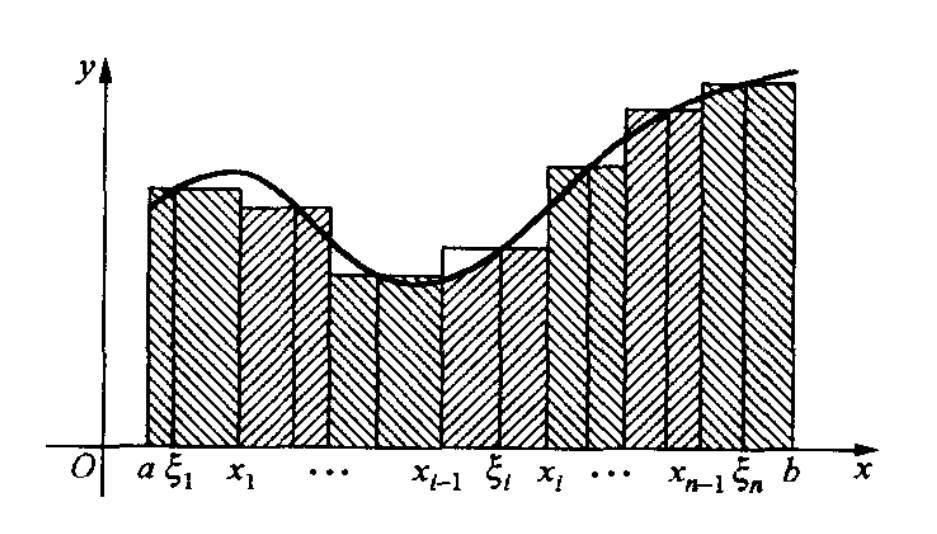
\includegraphics[width=\textwidth]{5.1.png} % 无需重复指定宽度  
\end{myimagebox}     
\caption{\label{fig:1.1}一致收敛的直观感受}   
\end{figure}

根据一致收敛的定义,我们可以得到如下推论:
\begin{tcolorbox}[
    colback=bac2,     % 极浅黄色背景
    colframe=fra2,   % 浅黄色边框
    coltitle=white,             % 标题文字白色
    coltext=tex2,
    title=利用强级数说明一致收敛,
    fonttitle=\bfseries,        % 标题加粗
arc=3mm,                     % 圆角稍大
breakable
]
\textbf{\color{brown!50!red}(推论16)利用强序列说明一致收敛}:给定$\{f_n(x)\},x\in D$,如果存在序列$\{u_n\}$,其中$\lim_{n\to+\infty}u_n=0$,且$|f_n(x)-f(x)|\leq |u_n|$,则$f_n(x)$一致收敛于$f(x)$。这个的原理很简单,因为$u_n$是与$x$无关的。
\end{tcolorbox}

\begin{tcolorbox}[
    colback=bac2,     % 极浅黄色背景
    colframe=fra2,   % 浅黄色边框
    coltitle=white,             % 标题文字白色
    coltext=tex2,
    title=利用反例序列说明不一致收敛,
    fonttitle=\bfseries,        % 标题加粗
arc=3mm,                     % 圆角稍大
breakable
]
\textbf{\color{brown!50!red}(推论17)寻找反例序列说明不一致收敛}:给定$\{f_n(x)\},x\in D$,如果存在$l>0$和序列$\{x_n\}\in D$,使得$|f_n(x_n)-f(x)|>l,\forall n\in\mathbb{N}$或者$\lim_{n\to+\infty}|f_n(x_n)-f(x_n)|=l$,则$f_n(x)$不一致收敛于$f(x)$。这是证明函数不一致收敛的重要办法。
\end{tcolorbox}


\textbf{\color{brown!50!red}例}:判断下列的函数序列是否一致收敛到极限函数。
\begin{align*}
    (1)f_n(x)=x^n\;x\in[0,1)\qquad
    (2)f_n(x)=\frac{n+x^2}{nx}\; x\in(0,1]\qquad
    (3)f_n(x)=\frac{n+x^2}{1+(nx)^2}\;x\in[0,1]
\end{align*}

第一个和第三个的极限函数都是0,第二个极限函数是$\frac{1}{x}$。第一个序列不一致收敛,我们可以找到点序列$x_n=1-\frac{1}{n}$,计算:
\begin{align*}
    \lim_{n\to\infty}|f_n(x)-f(x)|=\lim_{n\to\infty}(1-\frac{1}{n})^n=\frac{1}{e}>0
\end{align*}

对于第二个函数,由于:
\begin{align*}
    |f_n(x)-f(x)|=\frac{x^2}{nx}=\frac{x}{n}\leq\frac{1}{n}=u_n
\end{align*}

因此是一直收敛。对于第三个函数,寻找点序列$x_n=\frac{1}{n}$,则:
\begin{align*}
    |f_n(x)-f(x)|=\frac{1}{2}=l
\end{align*}

因此不一致收敛。然而利用推论16,17判断一致收敛也非常麻烦。接下来我们继续介绍一个定理:
\begin{tcolorbox}[
    colback=bac2,     % 极浅黄色背景
    colframe=fra2,   % 浅黄色边框
    coltitle=white,             % 标题文字白色
    coltext=tex2,
    title=一致收敛柯西定理,
    fonttitle=\bfseries,        % 标题加粗
arc=3mm,                     % 圆角稍大
breakable
]
\textbf{\color{brown!50!red}(定理18)一致收敛柯西定理}:给定函数序列$\{f_n(x)\},x\in D$,如果对$\forall \varepsilon>0,\exists N_\varepsilon$使得$|f_n(x)-f_m(x)|<\varepsilon,\forall n,m>N_\varepsilon,x\in D$,则原函数序列一致收敛。
\end{tcolorbox}

这个定理非常好证明,请自己完成。我们介绍下面的一个定义,它是我们常用的一个判别法的基础:给定函数集$\{f_n(x)\},x\in D$,定义\textbf{\color{brown!50!red}部分和函数}:$S_n=\sum_{k=1}^n f_k(x)$,$S_n(x)$有极限函数$S(x)$且一致收敛称作$\sum f_n(x)$收敛。我们看一个函数项级数$\sum x^n,x\in(-1,1)$,则其部分和为:$S_n(x)=\frac{1-x^{n-1}}{1-x}$,极限函数$S(x)=\frac{1}{1-x}$,因此:
\begin{align*}
    |S_n(x)-S_(x)|=\frac{|x|^{n-1}}{1-x}\geq \frac{1}{2}|x|^{n-1}
\end{align*}

我们找反例序列$x_n=1-\frac{1}{n}$,因此$|S_n(x)-S(x)|\geq \frac{1}{2}(1-\frac{1}{n})^{n-1}\to 2e^{-1}>0$,不一致收敛,证毕。

\begin{tcolorbox}[
    colback=bac2,     % 极浅黄色背景
    colframe=fra2,   % 浅黄色边框
    coltitle=white,             % 标题文字白色
    coltext=tex2,
    title=M判别法,
    fonttitle=\bfseries,        % 标题加粗
arc=3mm,                     % 圆角稍大
breakable
]
\textbf{\color{brown!50!red}(推论19)M判别法}:给定函数集$\{f_n(x)\},x\in D$,若存在\textbf{\color{brown!50!red}收敛的正项级数}$\sum u_n$,使得$|f_n(x)|\leq u_n$,则$S_n(x)$一致收敛。证明也很简单,因为$|S_m(x)-S_n(x)|\leq|\sum_{k=n+1}^m u_k(x)|$,根据定理3证毕。
\end{tcolorbox}

M判别法的应用非常广泛,因为我们只需要把函数$f_n(x)$向大放缩到与$x$无关的正数$u_n$,那么就变成了证明正项级数收敛的问题。我们看下面的一个函数项级数是否一致收敛:
\begin{align*}
    \sum_{n=1}^{+\infty}2^n\sin(\frac{1}{3^n(1+x^2)}),x\in \mathbb{R}
\end{align*}

由于$\sin$里面的值一定是大于0的,因此$\sin x<x$,并且$1+x^2\geq 1$,因此可以放大到$(2/3)^n$,这个等比级数收敛。和任意项级数的两种判别法一样,一致收敛也有狄利克雷判别法和阿贝尔判别法。我们先介绍“\textbf{\color{brown!50!red}一致有界}”的概念:对于$G_n(x)=\sum_{k=1}^n g_k(x)$,若$\forall n>0, x\in D$都有$|G_n(x)|\leq M$,称$G_n(x)$一致有界。
\begin{tcolorbox}[
    colback=bac2,     % 极浅黄色背景
    colframe=fra2,   % 浅黄色边框
    coltitle=white,             % 标题文字白色
    coltext=tex2,
    title=一致狄利克雷判别法,
    fonttitle=\bfseries,        % 标题加粗
arc=3mm,                     % 圆角稍大
breakable
]
\textbf{\color{brown!50!red}(定理20)一致狄利克雷判别法}:给定两个函数序列$\{f_n(x)\},\{g_n(x)\},x\in D$,如果对于$x\in D$固定,有$f_n(x)$关于$n$单调且$f_n(x)$一致收敛到0,并且$G_n(x)$一致有界,那么$\sum f_n(x)g_n(x)$一致收敛。
\end{tcolorbox}
\begin{tcolorbox}[
    colback=bac2,     % 极浅黄色背景
    colframe=fra2,   % 浅黄色边框
    coltitle=white,             % 标题文字白色
    coltext=tex2,
    title=一致阿贝尔判别法,
    fonttitle=\bfseries,        % 标题加粗
arc=3mm,                     % 圆角稍大
breakable
]
\textbf{\color{brown!50!red}(定理21)一致阿贝尔判别法}:给定两个函数序列$\{f_n(x)\},\{g_n(x)\},x\in D$,如果对于$x\in D$固定,有$f_n(x)$关于$n$单调且$f_n(x)$一致有界,并且$G_n(x)$一致收敛,那么$\sum f_n(x)g_n(x)$一致收敛。
\end{tcolorbox}

\textbf{\color{brown!50!red}证明一致收敛使用的是定理19,20,21}.\textbf{\color{brown!50!red}证明不一致收敛}通常是写出$|S_n(x)-S(x)|$,然后找反例序列,计算极限$|S_n(x_n)-S(x_n)|>0$,\textbf{\color{brown!50!red}利用了推理17}。

\textbf{\color{brown!50!red}例}:已知$x\in \mathbb{R}$,说明下面两个级数是否一致收敛。
\begin{align*}
    (1)\sum (-1)^{n-1}x^2e^{-nx^2}\qquad
    (2)\sum x^2e^{-nx^2}
\end{align*}

对于第一个级数我们使用定理20,令$g_n(x)=(-1)^{n-1}$,显然$G(x)$为$1/0$,一致有界。另一方面,如果我们固定$x$,那么$x^2e^{-nx^2}$关于$n$一定单调递减,并且$f_n(x)=\frac{1}{n}nx^2e^{-nx^2}\leq \frac{1}{n}\frac{nx^2}{1+nx^2}\leq \frac{1}{n}\Longrightarrow 0$,一致收敛到0。因此原级数一致收敛。

对于第二个级数,我们先计算部分和:
\begin{align*}
    S_n(x)=\sum_{k=1}^n x^2e^{-kx}=x^2\sum (e^{-x^2})^k=\frac{1-e^{-nx^2}}{1-e^{-x^2}}x^2e^{-nx^2}
 \end{align*}

 因此我们得到极限函数:
 \begin{align*}
     S_n(x)=\begin{cases}
         \frac{x^2}{e^{x^2}-1}&x\neq 0\\
         0&x=0\\
     \end{cases}
 \end{align*}

 当$x=0$,$S_n(0)-S(0)=0$;当$n\neq 0$时,则有:
 \begin{align*}
     |S_n(x)-S(x)|=|\frac{1-e^{-nx^2}}{1-e^{-x^2}}x^2e^{-nx^2}-\frac{x^2}{e^{x^2}-1}|=x^2e^{-x^2}\frac{e^{-nx^2}}{1-e^{-x^2}}
 \end{align*}

 我们取$x_n=\frac{1}{\sqrt{n}}$,因此$|S_n(x)-S(x)|=\frac{1}{n}\frac{1}{e(e^{1/n}-1)}\to \frac{1}{e}>0$,因此不是一致收敛的。

 \subsubsection{一致收敛的性质}
 我们继续看之前的一个例子$f_n(x)=x^n,x\in(0,1]$,这是不一致收敛的。我们发现对于任意取一个$n$,$x^n$是连续的;然而极限函数$f(x)$是在1处不连续的。因此我们称这种现象叫做“\textbf{\color{brown!50!red}不一致连续}”。因此我们给出下面的定理:
 \begin{tcolorbox}[
    colback=bac2,     % 极浅黄色背景
    colframe=fra2,   % 浅黄色边框
    coltitle=white,             % 标题文字白色
    coltext=tex2,
    title=一致收敛保连续,
    fonttitle=\bfseries,        % 标题加粗
arc=3mm,                     % 圆角稍大
breakable
]
\textbf{\color{brown!50!red}(定理22)一致收敛保连续}:设$f_n(x),x\in D$一致收敛于$f(x)$,且每个$f_n(x)$在定义域上连续,则$f(x)$也在定义域上连续。
\end{tcolorbox}

 这个定理的证明如下:我们取$x_0\in[a,b]$,对于任意的$\varepsilon>0$,我们找一个$\delta$,使得$|f(x)-f(x_0)|<\varepsilon,\forall |x-x_0|<\delta$。根据一致连续的几何意义,我们能找到一个$N_\varepsilon$,对于任意的$n>N_\varepsilon$,都能使$|f_n(x)-f(x)|<\varepsilon,\forall x\in D$。因此:
 \begin{align*} 
|f(x)-f(x_0)|&=|f(x)-f_n(x)+f_n(x)-f_n(x_0)+f_n(x_0)-f(x_0)|\\
&\leq |f(x)-f_n(x)|+|f_n(x)-f_n(x_0)|+|f_n(x_0)-f(x_0)|\\
&\leq 3\varepsilon 
\end{align*}

这个方法叫做在分析学中称作\textbf{\color{brown!50!red}三分法},在例题18中我们将进一步给出一致收敛保连续的完整解释。

因此如果说,\textbf{\color{brown!50!red}$f_n(x)$是连续的,但是极限函数不连续,我们就可以直接说不一致收敛}。因此上一章的最后一个例题就可以直接解决了,因为极限函数不是连续的。
\begin{tcolorbox}[
    colback=bac2,     % 极浅黄色背景
    colframe=fra2,   % 浅黄色边框
    coltitle=white,             % 标题文字白色
    coltext=tex2,
    title=一致收敛保积分,
    fonttitle=\bfseries,        % 标题加粗
arc=3mm,                     % 圆角稍大
breakable
]
\textbf{\color{brown!50!red}(定理23)一致连续保积分}:对于$f_n(x)$一致收敛于$f(x)$,且每一个$f_n(x)$在定义域上可积,则极限函数可积,且:
\begin{align*}
    \int_a^b f(x)\mathrm{d}x=\int_a^b \lim_{n\to\infty}f_n(x)\mathrm{d}x=\lim_{n\to\infty}\int_a^b f(x)\mathrm{d}x
\end{align*}
\end{tcolorbox}

这就是说,极限符号与积分符号可以互换!我们接下来进行如下证明:我们在这里证明:显然$|\int_a^b f(x)\mathrm{d}x-\int_a^b f_n(x)\mathrm{d}x|\leq \int_a^b |f(x)-f_n(x)|\mathrm{d}x$,对于$\forall \varepsilon,\exists N,|f(x)-f_n(x)|<\varepsilon$,因此左边$\leq \varepsilon(b-a)$,证毕。

我们接下来看一个不一致收敛的例子,并说明其极限和积分不可互换。对于函数:
\begin{align*}
    f_n(x)=\begin{cases}
        0 &x\in[\frac{1}{n},1]\\
        2n^2x &x\in[0,\frac{1}{2n}]\\
        2n^2(\frac{1}{n}-x) &x\in[\frac{1}{2n},\frac{1}{n}]
    \end{cases}
\end{align*}

它的极限函数为$0,x\in[0,1]$。因此极限函数的积分是0,然而对原函数的积分是$\frac{1}{2}$。同理我们可以寻找反序列。我们取$x_n=\frac{1}{2n}$,由于$\lim_{n\to\infty} |f_n(x)-f(x)|=n\to\infty$,因此是不一致收敛的。

那么一致收敛是否保导数?\textbf{\color{brown!50!red}这不一定}!我们看一个一致收敛的例子,$f_n(x)=\frac{x^n}{n},x\in[0,1]$,则极限函数$f(x)=0$,接下来由于$|f_n(x)-f(x)|\leq\frac
{1}{n}\to 0$,因此一致收敛。原函数的导数$f_n'(x)=x^{n-1}$,极限函数导数为0,因此一致收敛不一定保导数。我们接下来阐述一致收敛和导数的联系:
\begin{tcolorbox}[
    colback=bac2,     % 极浅黄色背景
    colframe=fra2,   % 浅黄色边框
    coltitle=white,             % 标题文字白色
    coltext=tex2,
    title=一致收敛保导数,
    fonttitle=\bfseries,        % 标题加粗
arc=3mm,                     % 圆角稍大
breakable
]
\textbf{\color{brown!50!red}(定理24)一致收敛和导数的联系}:设$x\in[a,b],f_n(x)$一致收敛到$f(x)$,且$f_n'(x)\in C^1[a,b]$(导数连续),并且在定义域上导数$f_n'(x)$也一致收敛到$g(x)$,则此时一致收敛保导数,即$\lim_{n\to\infty}f_n'(x)=f'(x)$,$f'(x)=g(x)$。
\end{tcolorbox}

我们接下来证明这个定理:由于一致收敛,因此$\lim(f_n(x)-f_n(a))\to f(x)-f(a)$,如果导数一致收敛,则左边为$\int_a^x f_n'(t)\mathrm{d}t$,右边为$\int_a^x g_n'(t)\mathrm{d}t$,因此$f'(x)=g(x)$。

所以这说明:如果原函数一致收敛,并且导函数也一致收敛并且连续,则求导计算和极限运算可以互换。一致收敛保积分和保导数可以用于级数求和。对于一个给定$\sum_{n=1}^\infty a_n(x)$,我们可以定义部分和函数$S_n(x)=\sum_{k=1}^\infty a_k(x)$,如果有极限函数$S(x)$,换言之,\textbf{\color{brown!50!red}原级数是收敛的},那么其实我们需要计算的是$S(x)$是多少。这本质上是对部分和求极限。因此我们可以选择积分——极限——求导或者求导——极限——积分的算法。

\textbf{\color{brown!50!red}例}:计算$\sum_{n=0}^\infty (n+1)x^n,x\in(-1,1)$。

我们先判断原函数是否收敛。对于$|x|<1$,原级数绝对收敛。我们定义部分和函数$S_n(x)=\sum_{n=0}^\infty (n+1)x^n$,则对于$\forall a\in[0,1),x\in(-a,a)$,部分和函数有极限函数$S(x)$。也就是说,$ \lim \int S_n(x)=\int S(x)$,即就是$S(x)=(\lim \int S_n(x))'$。则
\begin{align*}
    \int_{n=0}^x S(t)\mathrm{d}t&=\int_0^x  \sum_0^\infty  (n+1)t^n\mathrm{d}t\\
    &= \sum_0^\infty t^{n+1}|_0^x\\
    &=\frac{x}{1-x}
\end{align*}

因此$S(x)=(\frac{x}{1-x})'=\frac{1}{(1-x)^2},x\in[-a,a]$,所以原级数和为这个函数。

或者其实再简单一点,我们做的步骤就是:\textbf{\color{brown!50!red}先证明收敛,然后}\textbf{\color{brown!50!red}每一项积分,求和,再求导。}如果我们希望\textbf{\color{brown!50!red}每一项求导,求和,再积分},则要证明\textbf{\color{brown!50!red}原级数收敛,且导数是收敛连续}的。

\textbf{\color{brown!50!red}例}:计算级数和$\sum_{n=1}^\infty (-1)^{n-1}\frac{x^n}{n},x\in(-1,1]$。

这是一个交错级数,根据一致狄利克雷判别法,当$x\in(-1,1)$的时候,这个级数收敛。对每一项求导为$(-1)^{n-1}x^{n-1}$,求和为$\frac{1}{1+x}$,因此原级数和为$S(x)=\ln(1+x)+C$,由于$S(0)=0,C=0$。在$x=1$时,无法用莱布尼茨判别法,但是原级数简化为$(-1)^{n-1}\frac{1}{n}$,我们使用阿贝尔判别法,得到其级数和是收敛的。因此原函数一致收敛。根据一致收敛保连续,此时级数和为$\ln 2$。

(btw,数列有关收敛只是和n有关,函数项有关收敛和x,n都有关)

\subsection{泰勒展开有关级数}
\subsubsection{幂级数}
幂级数是形如$\sum_{n=0}^\infty u_n(x)=\sum_{n=0}^\infty a_n(x-x_0)^n$的级数,$x_0$是一定点。我们先介绍一个引理:

\begin{tcolorbox}[
    colback=bac2,     % 极浅黄色背景
    colframe=fra2,   % 浅黄色边框
    coltitle=white,             % 标题文字白色
    coltext=tex2,
    title=圆角框,
    fonttitle=\bfseries,        % 标题加粗
arc=3mm,                     % 圆角稍大
breakable
]
\textbf{\color{brown!50!red}(引理25)幂级数敛散的特性}:如果存在$x_1$使得$\sum a_nx_1^n$收敛,则对于$\forall x\in(-|x_1|,|x_1|),\sum a_nx^n$都是绝对收敛的;如果存在$x_2$使得$\sum a_nx_2^n$发散,则对于$\forall x\in(-\infty ,-|x_2);(|x_2|,+\infty),\sum a_nx^n$都是发散的。
\end{tcolorbox}

这个引理的证明如下:由于$\sum a_n x_1^n$绝对收敛,则当$x$在这个取值范围下,$\sum |a_nx^n|\leq \sum|a_n x_1^n|\cdot|x/x_1|^n\leq \sum |a_n x_1^n|$。注意我们没有要求在这个范围内收敛,而是\textbf{\color{brown!50!red}绝对收敛}。那么对于第二个问题,假设有$x_3$在这个区间内并且级数收敛,$(-|x_3|,|x_3)$这个范围内原级数绝对收敛。而在我们的$x_2$处是发散的,这是矛盾的。(回想一下,绝对收敛强于普通的条件收敛)

因此我们根据引理25可以发现,幂级数的收敛域有一个“半径”,称作收敛半径。我们对其的定义如下:

\begin{tcolorbox}[
    colback=bac2,     % 极浅黄色背景
    colframe=fra2,   % 浅黄色边框
    coltitle=white,             % 标题文字白色
    coltext=tex2,
    title=圆角框,
    fonttitle=\bfseries,        % 标题加粗
arc=3mm,                     % 圆角稍大
breakable
]
\textbf{\color{brown!50!red}(定义26)收敛半径}:给定幂级数$\sum_{n=0}^\infty a_nx^n$,一定存在$R\in[0,+\infty)$,使得幂级数在$(-R,R)$内绝对收敛,在$(-\infty,-R),(R,+\infty)$发散,在$R$处不确定
\end{tcolorbox}

\textbf{\color{brown!50!red}例}:分析幂级数$\sum_{n=1}^\infty (-1)^n \frac{x^n}{n+1}$的敛散性。

当$|x|<1$的时候,原级数根据莱布尼茨法则收敛。当$|x|>1$时级数发散。当$x=1$原级数收敛。$x=-1$原级数发散。所以收敛半径$R=1$,收敛域为$x\in(-1,1]$。

利用达朗贝尔判别法和柯西判别法本质上也能分析幂级数的敛散性。证明过程非常简单,我们直接介绍定理:
\begin{tcolorbox}[
    colback=bac2,     % 极浅黄色背景
    colframe=fra2,   % 浅黄色边框
    coltitle=white,             % 标题文字白色
    coltext=tex2,
    title=圆角框,
    fonttitle=\bfseries,        % 标题加粗
arc=3mm,                     % 圆角稍大
breakable
]
\textbf{\color{brown!50!red}(定理27)利用达朗贝尔判别法求收敛半径}:对于给定幂级数$\sum a_n x^n$,如果$\lim_{n\to\infty}|\frac{a_{n+1}}{a_n}|=l$,则收敛半径$R=\frac{1}{l}$(注:$l$可以取$0^+,+\infty$)
\end{tcolorbox}

\begin{tcolorbox}[
    colback=bac2,     % 极浅黄色背景
    colframe=fra2,   % 浅黄色边框
    coltitle=white,             % 标题文字白色
    coltext=tex2,
    title=圆角框,
    fonttitle=\bfseries,        % 标题加粗
arc=3mm,                     % 圆角稍大
breakable
]
\textbf{\color{brown!50!red}(定理28)利用柯西判别法求收敛半径}:对于给定幂级数$\sum a_n x^n$,如果$\lim_{n\to+\infty}\sqrt[n]{|a_n|}=l$,则收敛半径$R=\frac{1}{l}$。
\end{tcolorbox}

\textbf{\color{brown!50!red}例}:计算幂级数$\sum \frac{x^{n^2}}{2^n}$的收敛半径和收敛域。我们使用柯西判别法:

\begin{align*}
    \lim_{n\to+\infty}\sqrt[n]{|\frac{x^{n^2}}{2^n} |} =\frac{|x^n|}{2}=\begin{cases}
0 & |x|<1\\
\frac{1}{2}&|x|=1\\
+\infty &|x|>1 
\end{cases} 
\end{align*}

因此收敛半径为$R=1$。而在$x=\pm 1$都是收敛的。所以收敛域为$x\in [-1,1]$。幂级数有如下的性质:

\begin{tcolorbox}[
    colback=bac2,     % 极浅黄色背景
    colframe=fra2,   % 浅黄色边框
    coltitle=white,             % 标题文字白色
    coltext=tex2,
    title=圆角框,
    fonttitle=\bfseries,        % 标题加粗
arc=3mm,                     % 圆角稍大
breakable
]

\textbf{\color{brown!50!red}(定理29)幂级数的性质}:幂级数$\sum a_nx^n$与幂级数$\sum |a_n|x^n$的收敛半径相同。幂级数$\sum a_nx^n$与幂级数$\sum a_n n^mx^n$收敛半径相同($m>0$,是一个常数)。
\end{tcolorbox}

我们接下来对定理29进行证明:前一半是很简单的情况,我们只证后一半。设两个幂级数的收敛半径分别为$R_1,R_2$。那么$R_1\geq R_2$是显然的。因为当$n\to +\infty$时,$n^m>1$,所以根据比较判别法得知当$\sum a_nn^mx^n$收敛时$\sum a_nx^n$也一定收敛。接下来我们取$b\in(-R_1,R_1)$,则$\sum a_nx^n$在$[-b,b]$绝对收敛。因此对于$x\in(-b,b)$上,$\sum |a_nx^nn^m|=\sum|a_n b^n||n^m(x/b)^n|$,也是绝对收敛的。因此$R_2\geq b$。而$b$是任取的,因此$R_2\geq R_1$。因此我们证明了$R_1=R_2$。

幂函数之间四则运算与收敛半径的关系也有一些规律。接下来我们介绍:
\begin{tcolorbox}[
    colback=bac2,     % 极浅黄色背景
    colframe=fra2,   % 浅黄色边框
    coltitle=white,             % 标题文字白色
    coltext=tex2,
    title=幂函数收敛半径运算,
    fonttitle=\bfseries,        % 标题加粗
arc=3mm,                     % 圆角稍大
breakable
]
\textbf{\color{brown!50!red}(定理30)幂函数收敛半径运算}: 给定幂级数$\sum a_nx^n,\sum b_nx^n$,收敛半径分别是$R_a,R_b$,记$R=\min\{R_a,R_b\}$。则对于$\sum (a_n\pm b_n)x^n$的收敛半径$R_0$,如果$R_a\neq R_b$,则$R_0=R$;如果$R_a=R_b$,则$R_0\geq R$。对于$c_n=\sum_{j=0}^{n}a_jb_{n-j}$,幂级数$\sum c_nx^n$的收敛半径$R_0\geq R$。
\end{tcolorbox}

\begin{tcolorbox}[
    colback=bac2,     % 极浅黄色背景
    colframe=fra2,   % 浅黄色边框
    coltitle=white,             % 标题文字白色
    coltext=tex2,
    title=幂函数一致收敛性,
    fonttitle=\bfseries,        % 标题加粗
arc=3mm,                     % 圆角稍大
breakable
]
\textbf{\color{brown!50!red}(定理31)幂函数的一致收敛性}:对于给定的幂函数$\sum a_nx^n$与收敛半径R,若对于$\forall b\in(0,R)$,则幂函数在$[-b,b]$上一致收敛。如果在$R$处收敛,则幂函数在$[0,R]$一致收敛。如果在$-R$处收敛,则在$[-R,0]$上一致收敛。
\end{tcolorbox}

我们接下来证明定理31:如果$b\in(0,R)$,则$\sum |a_nx^n|=\sum|a_n r^n||(x/r)^n|\leq M_r|(b/r)^n|$,其中$b<r<R$。后面的正项等比级数是收敛的,因此前边的函数和(幂级数)也是收敛的。对于第二部分,$\sum a_nx^n=\sum a_n R^n(x/R)^n$,$(x/R)^n$是关于$n$单调递减且一致有界的。并且$\sum a_n R^n$收敛,因此由一致阿贝尔判别法得知原级数一致收敛。

因此像之前在一致收敛下进行函数和求和一样,幂级数这里也可以做相似的变换。给定幂级数$\sum a_nx^n$,收敛半径为$R$,记部分和函数$S(x)=\sum_{n=0}^\infty a_nx^n\; x\in(-R,R)$,则如果$S(x)$在$(-R,R)$上连续且幂级数$\sum a_nx^n$在$R$上收敛,则$S$在$(-R,R]$连续。在$-R$处类似。这其实就是\textbf{\color{brown!50!red}幂级数一致收敛保连续}。

幂函数由于自身的特殊性,它一致收敛保导数,并且保任意阶导数。即就是:
\begin{align*}
    S(x)^{(k)}=\sum_{n=0}^{+\infty}(a_nx^n)^{(k)}
\end{align*}

其在任意阶求导都满足内闭一致收敛。我们接下来看一个幂函数,分析其收敛半径,收敛域,并在收敛域下求和,解决第二个部分和:
\begin{align*}
    (1)\sum_{n=0}^{+\infty}\frac{2n+1}{2^n}x^{2n}  \qquad (2)\sum_{n=0}^{+\infty}\frac{(-1)^n}{2n+1}  
\end{align*}

对于第一个幂级数使用柯西判别法,$\lim \sqrt[n]{|\frac{2n+1}{2^n}x^{2n}|}=\frac{x^2}{2}<1$,因此收敛半径为$R=\sqrt{2}$,并且在$x=\pm \sqrt{2}$是发散的,因此收敛域为$(-\sqrt{2},\sqrt{2})$。求函数和采用积分——相加——求导的形式,每一项积分后的和为$\frac{x^{2n+1}}{2^n}$,求和为$\frac{2x}{1-x^2}$,然后求导得出$S(x)=2\frac{2+x^2}{(2-x^2)^2}$。

对于第二个级数和,考虑幂级数$\sum \frac{(-1)^n}{2n+1}x^{2n+1}$收敛半径为1,收敛域为$[-1,1]$。我们同样求导,求和,积分。逐项求导为$(-1)^n x^{2n}$,求和为$\frac{1}{1+x^2}$,积分后$S(x)=\arctan x+C$,根据$S(0)=0$确定$C=0$。然后这里$x=1$,因此原级数和为$S(1)=\frac{\pi}{4}$。我们用幂级数的敛散性来求级数和。

\subsubsection{泰勒级数}
在泰勒展开中,我们也许会想到:我能否一直展开,越来越趋近于原函数,并且原函数是否就是无尽展开的和?泰勒级数正是回答了这一点。我们介绍如下定理:

\begin{tcolorbox}[
    colback=bac2,     % 极浅黄色背景
    colframe=fra2,   % 浅黄色边框
    coltitle=white,             % 标题文字白色
    coltext=tex2,
    title=泰勒级数的参数,
    fonttitle=\bfseries,        % 标题加粗
arc=3mm,                     % 圆角稍大
breakable
]

\textbf{\color{brown!50!red}(定理32)泰勒级数的参数}:给定函数$f(x)$,设存在级数$\sum_{n=0}^\infty a_n(x-x_0)^n$以及某一个正数$r$,使得对于$\forall x\in(x_0-r,x_0+r)$都有:$\sum_{n=0}^{+\infty} a_n(x-x_0)^n=f(x),r\leq R$,则$f\in C^\infty (x_0-r,x_0+r)$,且有:
\begin{align*}
    a_n=\frac{f^{(n)}(x_0)}{n!} 
\end{align*}
\end{tcolorbox}

如果$f(x)$在$x_0$处无穷阶可导,那么就可以定义泰勒级数:
\begin{align*}
    f(x)\sim\sum_{n=0}^{+\infty}\frac{f^{(n)}(x_0)}{n!}(x-x_0)^n
\end{align*}

我们对于下面的函数计算泰勒级数:
\begin{align*}
    f(x)=\begin{cases}
        0&x=0\\
        e^{-\frac{1}{x^2}}& x\neq 0
    \end{cases}
\end{align*}

首先这个函数在$x=0$是无穷阶可导的。因此在0处的泰勒级数就是$\sum f^n\frac{x^n}{n!}$,而在0处的导数都是0,因此其泰勒级数为0,进一步收敛半径为$+\infty$。接下来我们介绍泰勒级数的余项:
\begin{tcolorbox}[
    colback=bac2,     % 极浅黄色背景
    colframe=fra2,   % 浅黄色边框
    coltitle=white,             % 标题文字白色
    coltext=tex2,
    title=泰勒级数的余项,
    fonttitle=\bfseries,        % 标题加粗
arc=3mm,                     % 圆角稍大
breakable
]
\textbf{\color{brown!50!red}(定义33)泰勒级数的余项}:对于给定的函数$f(x)$与泰勒级数,对于$\forall x\in[x_0-R,x_0+R]$,定义余项$R_n(x)=f(x)-\sum \frac{f^{(n)}(x_0)}{n!}(x-x_0)^n$。这里的余项有三种办法表示:
\begin{align*}
   R_n(x)=\begin{cases}
\circ((x-x_0)^n) &\text{佩亚诺余项}\\
\frac{f^{(n+1)}(x_0+\eta(x-x_0))}{(n+1)!}(x-x_0)^{n+1}&\text{拉格朗日余项}\\
\frac{f^{(n)}(x_0+\theta(x-x_0))}{n!}(1-\theta)^n(x-x_0)^{n+1}&\text{柯西余项}  
\end{cases} 
\end{align*}
\end{tcolorbox}

因此如果函数要等于它的泰勒级数,就要保证余项在$n\to\infty$的时候为0。同时要注意,泰勒级数本身是幂级数,存在收敛半径,因此函数等于它的泰勒级数的前提是定义域在收敛半径之内。

\textbf{\color{brown!50!red}例}:根据泰勒展开的形式去写出$e^x,\sin x,\cos x,\ln(1+x),(1+x)^\alpha$的泰勒级数,并且求出收敛半径和收敛域。
\begin{tcolorbox}[
    colback=bac1,     % 极浅橙色背景(几乎白色,但带暖调)
    colframe=fra1,   % 浅橙色边框(柔和)
    coltitle=white!80,    
    coltext=tex1,% 标题文字白色
    title=常见泰勒级数,
    fonttitle=\bfseries,        % 标题加粗
arc=2mm,                     % 轻微圆角
breakable
]
我们给出所有常见的泰勒级数:
\begin{align*}
  &e^x=\sum_{n=0}^{+\infty}\frac{x^n}{n!}\tag{5-2}\\
&\sin x=\sum_{n=0}^{+\infty}(-1)^n\frac{x^{2n+1}}{(2n+1)!}\tag{5-3}\\
&\cos x=\sum_{n=1}^{+\infty}(-1)^n\frac{x^{2n}}{(2n)!}\tag{5-4}\\
&\ln(1+x)=\sum_{n=1}^{+\infty}(-1)^{n+1}\frac{x^n}{n}\tag{5-5}\\
&(1+x)^\alpha=\sum_{n=0}^{+\infty}\frac{\alpha(\alpha-1)...(\alpha-n+1)}{n!}x^n \tag{5-6}     
\end{align*}
\end{tcolorbox}

接下来我们来分析等号是否成立,在何时成立。对于$e^x$而言,余项有:
\begin{align*}
  |R_n(x)|=|\frac{e^{\eta x}}{(n+1)!}x^{n+1}|\to 0    
\end{align*}

对于任意的$x$,余项都是趋近于0,因此收敛半径$R=+\infty$。而对$\sin x$的余项为:
\begin{align*}
  |R_n(x)|=|\frac{\cos(\eta x)}{(2n+3)!}x^{2n+3}|\to 0    
\end{align*}

对于任意的$x$,余项都是趋近于0,因此收敛半径$R=+\infty$。而对于$\ln(1+x)$的余项也如此。但是注意由于$x>-1$,因此收敛半径只能为1,收敛域为$x\in(-1,1]$。而对于$(1+x)^\alpha$,考虑\colorbox{pink!30!white}柯西余项:
\begin{align*}
  |R_n(x)|=\left|\frac{\alpha(\alpha-1)...(\alpha-n)}{n!}x^{n+1}(1+\theta x)^{\alpha-1}
\left(\frac{1-\theta}{1+\theta x} \right)^n \right|
\end{align*}

余项是由4项组成的,我们需要考虑在$n\to\infty$时余项趋近于0的条件。首先当$|x|<1$的时候,无论$\alpha$取值为多少,第一项是有界的,第二项趋近于0,第三项是常数,第四项绝对值在$|x|<1$的时候也是趋近于0的,所以余项趋近于0,也就是说无论$\alpha$为多少,原泰勒级数都在$(-1,1)$绝对收敛。

当$x=\pm 1$的时候,我们需要考虑:
\begin{align*}
  |R_n(x)|=\left|\frac{\alpha(\alpha-1)...(\alpha-n)}{n!}\right|
\end{align*}

是否趋近于0,此时我们关注:$\sum_{n=0}^{+\infty} 
|R_n|$是否收敛。如果收敛就可以证明其趋近于0,如果不收敛也不一定。这个级数使用\colorbox{pink!30!white}拉阿伯判别法:
\begin{align*}
    \lim_{n\to+\infty}n\left(\frac{|u_n|}{|u_{n+1}|}-1\right)=\lim_{n\to+\infty}\frac{n(1+\alpha)}{n-\alpha}
\end{align*}

在大于1的时候才能收敛,因此$\alpha>0$,也就是说,在$\alpha>0$时收敛域为$[-1,1]$。而当$\alpha<0$时又怎么样呢?是否存在条件收敛?因为如果有条件收敛的话,也可以证明$|R_n|\to0$,当$n$足够大的时候,$u_{n+1}/u_n=\frac{\alpha-n}{n+1}<0$是交错级数。在$x=1$我们还是研究上面的级数,用莱布尼茨判别法,则$\alpha>-1$才能使条件收敛成立。如果$x=-1$,$u_{n+1}/u_n=\frac{\alpha-n}{n+1}>0$,不是交错级数了。因此不收敛。因此我们总结一下结论:$\alpha>0$,收敛域$[-1,1]$;$-1<\alpha<0$,收敛域$(-1,1]$;$\alpha\leq -1$,收敛域$(-1,1)$。

对于$\arcsin x,\arctan x$的泰勒展开,我们可以进行\colorbox{pink!30!white}求导后展开再积分的方法,易得到:
\begin{align*}
   &\arctan x=\sum_{n=0}^{+\infty}(-1)^n\frac{x^{2n+1}}{2n+1}\qquad x\in[-1,1]\tag{5-7}\\
 &\arcsin x=\sum_{n=0}^{+\infty}\frac{(2n-1)!!}{(2n)!!}\frac{x^{2n+1}}{2n+1}\qquad x\in[-1,1]\tag{5-8}\\
 &\ln(\frac{1+x}{1-x})=2\sum_{n=0}^{+\infty}\frac{x^{2n+1}}{2n+1}\qquad x\in(-1,1)\tag{5-9}
\end{align*}

\subsection{习题补充与扩展}
本章内容极多,技巧及丰富,应用极广泛,不想看习题可直接跳转。

在本章习题开始前,我们先介绍Strling公式和Wallis公式:
\begin{tcolorbox}[
    colback=bac1,     % 极浅橙色背景(几乎白色,但带暖调)
    colframe=fra1,   % 浅橙色边框(柔和)
    coltitle=white!80,    
    coltext=tex1,% 标题文字白色
    title=Strling公式与Wallis公式,
    fonttitle=\bfseries,        % 标题加粗
    arc=2mm,                    % 轻微圆角
    breakable
]
\begin{align*}
    &n!\sim \sqrt{2\pi n}(\frac{n}{e})^n\\
    &\frac{2n!!}{(2n-1)!!}\sim\sqrt{\pi n}
\end{align*}
\end{tcolorbox}

\textbf{\color{brown!50!red}例1}:尝试证明正项级数收敛的两个判别法:

(1)\textbf{\color{brown!50!red}Sapagof判别法}:设正数数列$\{a_n\}$单调递减,则$\lim_{n\to+\infty} a_n=0$的充要条件为正项级数$\sum_{n=1}^\infty (1-\frac{a_{n+1}}{a_n})$发散。

(2)\textbf{\color{brown!50!red}Kummer判别法}:正项级数$\sum_{n=1}^\infty a_n$收敛的充要条件是存在正数数列$\{b_n\}$和正数$\delta$,当$n$充分大的时候下式成立:
\begin{align*}
    b_n\frac{a_n}{a_{n+1}}-b_{n+1}\geq\delta>0
\end{align*}

\textbf{\color{brown!50!red}解}:(1)不妨令$b_n=1-\frac{a_{n+1}}{a_n}$,由于$\{a_n\}$单调递减,则$\lim_{n\to\infty}a_n=a$,有下界。这里利用假如令$a> 0$,则移项可得:$b_n\leq \frac{a_n-a_{n+1}}{a}$。而:
\begin{align*}
    \sum_{n=1}^\infty b_n=\frac{1}{a}\sum_{n=1}^\infty(a_n-a_{n+1})=\frac{1}{a}(a_1-a)
\end{align*}

所以$\sum b_n$是收敛的。如果$a=0$,则我们计算部分和:
\begin{align*}
\sum_{k=n+1}^{n+p}b_k=\sum_{k=n+1}^{n+p}\frac{a_k-a_{k+1}}{a_k}\geq \frac{a_k-a_{k+1}}{a_{n+1}}=1-\frac{a_{n+p+1}}{a_{n+1}}
\end{align*}

对于每一个给定的$n$,我们总可以找到一个充分大的$p$,使得上面的式子大于$\frac{1}{2}$,利用柯西收敛准则得知级数发散。

(2)先证充分性,由不等式推导收敛。原不等式可以改写为:
\begin{align*}
    0<\delta a_{n+1}\leq b_na_n-b_{n+1}a_{n+1}
\end{align*}

因此正项数列$\{b_na_n\}$是单调递减的。因此:
\begin{align*}
    \sum_{k=1}^\infty a_k\leq a_1+\frac{1}{\delta}\sum_{k=1}^\infty (b_ka_k-b_{k+1}a_{k+1})\leq a_1+\frac{1}{\delta}b_1a_1
\end{align*}

因此原级数是收敛的。然后证明必要性,记$R_n=\sum_{k=1}^\infty a_k-\sum_{k=1}^n a_k,b_n=\frac{R_n}{a_n}$,因此原式可以写作:
\begin{align*}
    b_n\frac{a_n}{a_{n+1}}-b_{n+1}=\frac{R_n-R_{n+1}}{a_{n+1}}=1=\delta
\end{align*}

\textbf{\color{brown!50!red}例2}:讨论下面级数的敛散性
\begin{align*}
    (1)\sum_{n=2}^\infty \frac{1}{(\ln n)^{\ln n}}\qquad
   (2)\sum_{n=1}^\infty \left[ \frac{(2n-1)!!}{2n!!}\right]^k\qquad
   (3) n!(\frac{a}{n})^n(a>0)
\end{align*}

\textbf{\color{brown!50!red}解}:对于第一题,由于:
\begin{align*}
    a^{\ln b}=e^{\ln a\ln b}=b^{\ln a}
\end{align*}

因此第一个级数可以化作:
\begin{align*}
    \sum\frac{1}{\ln n^{\ln n}}=\sum\frac{1}{n^{\ln(\ln n)}}
\end{align*}

当$n>e^{e^2}$的时候,分母大于$n^2$,由于$\sum \frac{1}{n^2}$发散,因此原级数是发散的。对于第二个题,使用Wallis公式可得:
\begin{align*}
    \sum_{n=1}^\infty \left[ \frac{(2n-1)!!}{2n!!}\right]^k=\sum\frac{1}{(\pi n)^{k/2}}
\end{align*}

因此当$k\geq 2$的时候是发散的,$k<2$是收敛的。对于第三个题,由于:
\begin{align*}
    a_n=n!(\frac{a}{n})^n\sim(\frac{a}{e})^n\sqrt{2\pi n}=b_n
\end{align*}

当$a\geq e$的时候,显然$b_n\to 0$不成立,因此级数发散的。当$a<e$时,取$r\in(\frac{a}{e},1)$则有:
\begin{align*}
    \sum b_n<\sum r^n\sqrt{2\pi n}
\end{align*}

这显然是发散的,因此原级数发散。

\textbf{\color{brown!50!red}例3}:(1)设正项级数$\sum_{n=1}^{+\infty}a_n$的部分和数列为$\{S_n\}$,且$p>1$,证明$\sum_{n=1}^{+\infty}\frac{a_n}{S_n^p}$收敛。

(2)设正项级数$\sum_{n=1}^\infty\frac{1}{a_n}$收敛,$\{a_n\}$是单调递增的(实际上接下来的结论不需要这一点,只是这需要一个初等结论)。证明下面的级数收敛:
\begin{align*}
    \sum_{n=1}^\infty \frac{n}{a_1+a_2+...+a_n}
\end{align*}

\textbf{\color{brown!50!red}解}:(1)首先我们需要证明一个不等式,即就是:
\begin{align*}
    \frac{1}{a^{p-1}}-\frac{1}{b^{p-1}}>(p-1)\frac{b-a}{b^p}
\end{align*}

假设这个不等式成立,代入$a=S_{n-1},b=S_n$,则有:
\begin{align*}
    \frac{a_n}{S_n^p}=\frac{S_n-S_{n-1}}{S_n^p}<\frac{1}{p-1}\left(\frac{1}{S_{n-1}^{p-1}}-\frac{1}{S_n^{p-1}}\right)
\end{align*}

因此原级数和为:
\begin{align*}
    \sum_{k=1}^\infty\frac{a_k}{S_k^p}&=\frac{1}{a_1^{p-1}}+\sum_{k=2}^\infty\frac{a_k}{S_k^p}<\frac{1}{a_1^{p-1}}+\frac{1}{p-1}\sum_{k=2}^\infty\left(\frac{1}{S_{k-1}^{p-1}}-\frac{1}{S_k^{p-1}}\right)\\
    &<\frac{1}{a_1^{p-1}}+\frac{1}{p-1}\frac{1}{a_1^{p-1}}=\frac{p}{p-1}\frac{1}{a_1^{p-1}}
\end{align*}

因此我们证明了收敛。接下来我们要说明不等式的正确性。设$0<a<b$,对函数$x^{1-p},x\in[a,b]$上使用拉格朗日中值定理,得到:
\begin{align*}
    \frac{1}{a^{p-1}}-\frac{1}{b^{p-1}}=\frac{(p-1)}{\xi^p}(b-a)>\frac{b-a}{b^p}(p-1)
\end{align*}
\begin{tcolorbox}[
    colback=bac1,     % 极浅橙色背景(几乎白色,但带暖调)
    colframe=fra1,   % 浅橙色边框(柔和)
    coltitle=white!80,    
    coltext=tex1,% 标题文字白色
    title=注意,
    fonttitle=\bfseries,        % 标题加粗
arc=2mm,                     % 轻微圆角
breakable
]
拉格朗日中值定理在这里非常常见,我们的$p$级数证明也用到了拉格朗日中值定理。此外这个不等式的结果要格外重视!
\end{tcolorbox}

(2) 如果$\{a_n\}$单调递增,则有:
\begin{align*}
&a_1+a_2+...+a_{2n-1}\leq a_n+a_{n+1}+...+a_{2n-1}\leq na_n\\
&\frac{2n-1}{a_1+a_2+...+a_{2n-1}}+\frac{2n}{a_1+a_2+...+a_{2n}}\leq \frac{2n-1}{na_n}+\frac{2n}{na_n}\leq 4\frac{1}{a_n}
\end{align*}

因此部分和有上界,因此收敛。这有点类似于正项级数中的第$2n-1,2n$项之和小于4倍的第$n$项。

\textbf{\color{brown!50!red}例4}:判断下面级数的敛散性。
\begin{align*}
    &(1)\sum_{n=1}^\infty \left[\frac{1}{n}-\ln{(1+\frac{1}{n})}\right] &(2)\sum_{n=1}^\infty\frac{n^{n-1}}{(2n^2+n+1)^{\frac{n-1}{2}}}\\
    &(3)\sum_{n=2}^\infty \frac{n^{\ln n}}{(\ln n)^n} 
    &(4)\sum_{n=1}^\infty (1-\frac{\ln n}{n})^n
\end{align*}

\textbf{\color{brown!50!red}解}:(1)当$n$足够大的时候,根据泰勒展开可以得到:
\begin{align*}
    \frac{1}{n}-\ln(1+\frac{1}{n})<\frac{1}{n}-(\frac{1}{n}-\frac{1}{2n^2})=\frac{1}{2n^2}
\end{align*}

因此原级数是收敛的。

(2)利用柯西判别法:
\begin{align*}
    \lim_{n\to\infty}\sqrt[n]{a_n}&=\frac{n^{1-\frac{1}{n}}}{(2n^2+n+1)^{\frac{1}{2}-\frac{1}{2n}  }}
\\&=\left(\frac{n^2}{2n^2+n+1}\right)^{\frac{1}{2} } \left(\frac{n^2}{2n^2+n+1}\right)^{-\frac{1}{2n} }
\\&=\frac{1}{\sqrt{2}}<1 
\end{align*}


因此原级数是收敛的。

(3)使用柯西判别法:
\begin{align*}
    \lim_{n\to\infty}\sqrt[n]{a_n}&=\exp[\frac{1}{n} [(\ln n)^2-n\ln(\ln n)]]\\
&=\exp[(e^{-t}t^2-\ln t)]=0
\end{align*}

因此原级数收敛。

(4)进行指数变换得到近似于$\frac{1}{n}$,发散。

\textbf{\color{brown!50!red}例5}:(1)设$x>0$,证明下面的级数是收敛的:
\begin{align*}
    \sum_{n=1}^\infty \frac{x^n}{(1+x)(1+x^2)...(1+x^n)}
\end{align*}

(2)设数列$\{a_n\}$单调递减,且$\lim_{n\to+\infty}a_n=0$,并且$b_n=a_n-2a_{n+1}+a_{n+2}\geq 0,\forall n\in\mathbb{N}^+$,证明下面的级数收敛,且有:
\begin{align*}
    \sum_{n=1}^\infty nb_n=a_1
\end{align*}

\textbf{\color{brown!50!red}解}:(1)求级数和的另一种办法是裂项:
\begin{align*}
   a_n&=\frac{1}{(1+x)(1+x^2)+...(1+x^{n-1})}-\frac{1}{(1+x)(1+x^2)+...(1+x^{n})} \\
\sum a_n&=\frac{x}{1+x}+\frac{1}{1+x}-\lim_{n\to\infty}\frac{1}{(1+x)...(1+x^n)}=1  
\end{align*}

(2)记$c_n=a_n-a_{n+1}$,因此$b_n=c_n-c_{n+1}\geq 0$,而$\sum c_n=a_1-\lim_{n\to\infty}a_n=a_1$,因此$\sum c_n$收敛,根据Cauchy收敛准则有:
\begin{align*}
    0<C_{N+1}+C_{N+2}+...+C_n<\frac{\varepsilon}{2}
\end{align*}

取$n>2N$,则:
\begin{align*}
    &0<\frac{n}{2}c_n\leq (n-N)c_n<\frac{\varepsilon}{2}\\
    &0<nc_n<\varepsilon\qquad nc_n\to 0
\end{align*}

因此我们要计算的级数和为:
\begin{align*}
    \sum_{n=1}^\infty nb_n=\sum_{n=1}^\infty n(c_n-c_{n+1})=\lim_{n\to+\infty}(\sum_{k=1}^n c_k-(k+1)c_{k+1})=a_1
\end{align*}

\textbf{\color{brown!50!red}例6}:当$x\in(0,e)$时,讨论下方级数的敛散性:
\begin{align*}
    \sum_{n=1}^\infty(2-x)(2-x^{\frac{1}{2}})...(2-x^\frac{1}{n})
\end{align*}

\textbf{\color{brown!50!red}解}:当$x\in(0,1]$时,每一项一定都是大于1的,因此一定发散。当$x=2$时,每一项都是0,一定收敛。

当$x\in(0,1),(2,e)$时,利用拉阿伯判别法:
\begin{align*}
  n(\frac{u_n}{u_{n+1}}-1)&=n(\frac{1}{2-x^{\frac{1}{n+1}}}-1)=n\frac{x^{\frac{1}{n+1}-1}}{2-x^\frac{1}{n+1}}\\
&\to n\exp[\frac{1}{n+1}\ln(x)-1]\to \ln x
\end{align*}

因此原级数是发散的。显然在$x>e$是收敛的。在$x=e$没办法确定。

\textbf{\color{brown!50!red}例7}:设数列$\{a_n\}$单调递减且极限为0,级数$\sum_{n=1}a_n$发散,证明当$x\neq k\pi,k=\pm1,\pm2...$时,下面的级数是条件收敛的:
\begin{align*}
    \sum_{n=1}^\infty a_n\sin nx
\end{align*}

\textbf{\color{brown!50!red}解}:使用狄利克雷判别法,由于$\{a_n\}$单减趋于零,因此我们只需要说明$\sum \sin nx$部分和有界。由于:
\begin{align*}
    2\sin\frac{x}{2}(\sin x+\sin 2x+...+\sin nx)=\cos\frac
    {x}{2}-\cos\frac{(2n+1)x}{2}
\end{align*}

因此得到部分和:
\begin{align*}
    |\sin x+\sin 2x+...+\sin nx|\leq\frac{1}{|\sin \frac{x}{2}|}
\end{align*}

因此部分和是有界的,因此级数是收敛的。另一方面,$|a_n\sin nx|\geq a_n\sin^2 nx=\frac{1}{2}(a_n-a_n\cos 2nx)$,由于$\sum a_n\cos 2nx$是收敛的,$\sum a_n$发散,因此不等式右侧发散,根据比较判别法得知左侧是发散的。证毕。

\textbf{\color{brown!50!red}例8}:判断下面级数的条件收敛性和绝对收敛性。
\begin{align*}
    &(1)\sum_{n=1}^\infty (-1)^n\frac{\cos^2 n}{n} &(2)\sum_{n=1}^\infty\frac{\sin nx}{n}(1+\frac{1}{n})^n\\
    &(3)\sum_{n=1}^\infty (1+\frac{1}{2}+..+\frac{1}{n})\frac{\sin nx}{n}&(4)\sum_{n=1}^\infty \sin(\pi\sqrt{n^2+a^2})
\end{align*}

解:(1)先判断是否绝对收敛,利用二倍角公式得到:
\begin{align*} 
  \sum\frac{\cos^2 n}{n}=\sum \frac{1}{2n}+\sum\frac{\cos 2n}{2n}
\end{align*}

前面这一部分是发散的,后边这一部分$\frac{1}{2n}$单调递减趋近于0,$\sum \cos 2n$时有界的(参考例题7),因此收敛,则整体是发散的,并非绝对收敛。再考虑条件收敛,利用诱导公式:
\begin{align*} 
  \sum(-1)^n\frac{\cos^2 n}{n}=\sum \frac{\cos(2n+n\pi)}{2n}   
\end{align*}

这个级数是收敛的,因此原级数条件收敛。

(2)当$x=k\pi$时,级数每一项都是0,绝对收敛。反之,$\sum \sin nx$是有界的,而:
\begin{align*} 
 & a_n=\frac{(1+\frac{1}{n})^n }{n}=\exp[n\ln(1+\frac{1}{n})-\ln n]\\
 &a_n'<0\qquad \lim_{n\to+\infty}a_n=\frac{e}{n}\to 0 
\end{align*}

因此是单调递减趋于0,根据狄利克雷判别法得知其条件收敛。而由于$(1+\frac{1}{n})^n\geq 1$,而$\sum |\frac{\sin nx}{n}|$是发散的,这是因为,令$x=k\pi+m$,则$|\sin nx=\sin n(k\pi+m)=\sin nm|$,则就有:
\begin{align*} 
 \sum\frac{|\sin nx|}{n}\geq \sum a_n\\
a_n=\begin{cases}
0 & |\sin nx|\neq |\sin m|\\
\frac{|\sin m|}{n} &|\sin nx|=|\sin m|
\end{cases} 
\end{align*}

后面的级数发散,因此原级数不是绝对收敛的、

(3)先判断条件收敛,由狄利克雷判别法易得其条件收敛。对于绝对收敛,由于$(1+\frac{1}{2}+...+\frac{1}{n})>\ln(n+1)$,根据(2)得知其绝对收敛。

(4)利用诱导公式变形:
\begin{align*} 
 \sum\sin(\pi\sqrt{n^2+a^2})=\sum(-1)^n\sin(\pi\sqrt{n^2+a^2}-n\pi)=
\sum(-1)^n\sin(\pi\frac{a^2}{\sqrt{n^2+a^2}+n})
\end{align*}

根据莱布尼茨判别法可知其条件收敛。对于绝对收敛,当$n$足够大,使得正弦内部小于$\frac{\pi}{2}$,由于:
\begin{align*}
    \sin\theta\geq\frac{2\theta}{\pi}(\theta\in[0,\frac{\pi}{2}])
\end{align*}

\begin{align*} 
 \sum_{n=1}^\infty\sin(\pi\frac{a^2}{\sqrt{n^2+a^2}+n})>\sum_{n=N}^\infty\frac{2a^2}{\sqrt
{n^2+a^2} +n}>\sum_{n=N}\frac{a^2}{2\sqrt{n^2+a^2}}  
\end{align*}

因此它不是绝对收敛的。

\textbf{\color{brown!50!red}例9}:假设$p,q>0$讨论下面两个级数的敛散性。
\begin{align*}
    &(1)1-\frac{1}{2^q}+\frac{1}{3^p}-\frac{1}{4^q}+...\\
    &(2)\sum_{n=1}^\infty\frac{(-1)^n(1+p)(2+p)...(n+p)}{n!n^q}
\end{align*}

\textbf{\color{brown!50!red}解}:(1)我们考虑它的一个正负部。\textbf{\color{brown!50!red}当正负部级数都收敛时,原级数绝对收敛(充要条件)。当一个收敛另一个发散的时候,原级数肯定发散。当两个都发散的时候,对于条件收敛需要进一步分析}。
\begin{align*} 
 \sum_{n=1}^\infty a_n^+=\sum_{n=1}^\infty \frac{1}{(2n-1)^p}\qquad  
\sum_{n=1}^\infty a_n^-=\sum_{n=1}^\infty \frac{1}{(2n)^q}  
\end{align*}

显然当$p,q>1$原级数是绝对收敛的;当$p\leq 1,q>1;p>1,q\leq 1$原级数发散。当$p,q<\leq 1$的时候,先考虑最简单的情况$p=q$,根据莱布尼茨判别法得知原级数条件收敛。而当$p\neq q$的时候,给原级数插入$\frac{1}{2^p},\frac{1}{4^p}...$改写成:
\begin{align*} 
 \sum_{n=1}^\infty a_n=\sum_{n=1}^\infty\frac{(-1)^{n-1}}{n^p}+\sum_{n=1}^\infty\left[
\frac{1}{(2n)^p}-\frac{1}{(2n)^q}  \right] 
\end{align*}

第一部分根据莱布尼茨判别法得知收敛。第二部分是发散的。因此原级数发散。

(2)原式可以写作:
\begin{align*} 
 \frac{(-1)^n(1+p)(2+p)...(n+p)}{n!n^q}&=(-1)^n\exp\left[\sum_{k=1}^n
\ln(1+\frac{p}{k})\right]  \cdot\frac{1}{n^q}\\
&=(-1)^n\frac{\exp\left[p\sum_{k=1}^{^n}\frac{1}{k}+\sum_{k=1}^nO(\frac{1}{k^2}) \right]}{n^q}\\
&=(-1)^n\frac{\exp[C+p\ln n+O(1)]}{n^q} \\
&=(-1)^n\frac{e^{C+O(1)}}{n^{q-p}} 
\end{align*}

$q-p>1$绝对收敛,$p<q\leq p+1$条件收敛,其余情况发散。

\textbf{\color{brown!50!red}例10}:研究下列级数的绝对收敛和条件收敛性质,如果分母为0则去掉这一项。
\begin{align*}
    \sum_{n=1}^\infty\frac{1}{1+nx^n}
\end{align*}

\textbf{\color{brown!50!red}解}:当$x>1$的时候,$n$足够大时$\sum a_n>\frac{1}{n^2}$,因此发散。$x=1$时,$\sum\frac{1}{1+n}$发散。$x\in(-1,1)$时,极限为1,发散。$x=-1$,根据莱布尼茨判别法得知其条件收敛,而$\sum\frac{1}{n-1}$并非绝对收敛。当$x<-1$时,$x$足够大的时候,$a_n<\frac{1}{n^2}$,因此绝对收敛。

\textbf{\color{brown!50!red}例11}:(1)已知级数$\sum_{n=1}^\infty a_n$发散,证明:$\sum_{n=1}^\infty (1+\frac{1}{n})a_n$也发散。

(2)证明\textbf{\color{brown!50!red}Du Bois-Reymond判别法}:设级数$\sum_{n=2}^\infty(a_n-a_{n-1})$绝对收敛,且$\sum_{n=1}^\infty b_n$收敛,则$\sum_{n=1}^\infty a_nb_n$收敛。

\textbf{\color{brown!50!red}解}:(1)我们不妨令$b_n=(1+\frac{1}{n})a_n$,则$a_n=\frac{n}{n+1}b_n$。假如$\sum b_n$是收敛的,由于$\frac{n}{n+1}$是单调递增的并且有上界,因此$\sum a_n$也收敛,这产生了矛盾。

(2)我们不妨令$B_n=b_1+b_2+...+b_n$,做Abel变换则有:
\begin{align*} 
 \sum_{k=1}^n a_nb_n=\sum_{k=1}^{n-1}B_k(a_k-a_{k+1})+B_na_n
\end{align*}

由于$\sum b_n$收敛,因此$B_n$有界,且$|B_n|\leq M$。又因为$\sum a_n-a_{n-1}$绝对收敛,则:
\begin{align*}
    \lim_{n\to\infty}a_n=a_1+\sum(a_n-a_{n-1})<a_1+c
\end{align*}

因此等式右边是有界的,所以原级数收敛。

\textbf{\color{brown!50!red}例12}:(1)设函数$f(x)$是在$[1,+\infty)$的非负单调递减函数,则证明下面极限$A$存在且$0\leq A\leq f(1)$。
\begin{align*}
    \lim_{n\to\infty}\left(\sum_{k=1}^\infty f(k)-\int_1^n f(x)\right)=A
\end{align*}

(2)求证下面的极限成立:
\begin{align*}
    \lim_{n\to+\infty}\frac{x^2}{x^2+n^2}=\frac{\pi}{2}
\end{align*}

\textbf{\color{brown!50!red}解}:(1)考虑到定积分分段积分,则有:
\begin{align*} 
 a_n&=\sum_{k=1}^nf(k)-\sum_{k=1}^{n-1}\int_{k}^{k+1}f(x)\mathrm{d}x\\
&\geq \sum_{k=1}^n f(k)-\sum_{k=1}^{n-1}f(k)\cdot1\\
&=f(n)\geq 0
\end{align*}

而在另一边:
\begin{align*} 
 a_{n+1}-a_n&=f(n+1)-\int_{n}^{n+1}f(x)\mathrm{d}x\\
&\leq  f(n+1)-f(n+1)=0
\end{align*}

因此单调递减有下界,下界就是极限$A$,并且$0\leq A\leq f(1)$得证。

(2)我们令这里有:
\begin{align*}
    f(y)=\frac{x}{x^2+y^2}
\end{align*}

则$f(1)=\frac{x}{x^2+1}$,$x\to\infty$时趋近于0,因此$A=0$,进一步就有:
\begin{align*}
    \int_1^nf(y)\mathrm{d}y=\frac{\pi}{2}-\arctan{\frac{1}{x}}\to\frac{\pi}{2}
\end{align*}

因此原式就是其加上A的极限,证毕。

\textbf{\color{brown!50!red}例13}:(1)设级数$\sum na_n$收敛,证明对任意正整数$k$都存在$\sum na_{n+k}$收敛。

(2)设$a>0,a_n\geq 0$,证明下方级数收敛,且和$S\leq \frac{a}{\sqrt{2}}$。
\begin{align*}
    \sum_{n=1}^\infty \frac{a_n}{(a_1+a_2+...+a_n)^{3/2}}
\end{align*}

\textbf{\color{brown!50!red}解}:第一题只需要换标即可。
\begin{align*} 
 \sum_{n=1}^\infty na_{n+k}=\sum_{n=1+k}^\infty(n-k)a_n=\sum_{n=1+k}^\infty na_n(1-\frac{k}{n})
\end{align*}

由Abel判别法,单调有界+级数收敛,证毕。对于第二题,记$S_n=a+a_1+a_2+...+a_n$,则:
\begin{align*} 
 \frac{a_n}{S_n^{p}}=\frac{S_n-S_{n-1}}{S_n^{p}}<\frac{1}{p-1}(\frac{1}{S_{n-1}^{p-1}}-
\frac{1}{S_n^{p-1}}  )  
\end{align*}

这一步是使用了拉格朗日中值定理。因此原级数变为:
    \begin{align*} 
 \sum_{n=1}^\infty\frac{a_n}{S_n^{3/2}}&=\frac{a_1}{(a_1+a)^{3/2}}  +\sum_{n=2}^\infty\frac{a_n}{S_n^{3/2}}\\
&<\frac{a_1}{(a_1+a)^{3/2}}+2\sum_{n=2}^\infty(\frac{1}{S_{k-1}^{1/2}}- \frac{1}{S_{k}^{1/2}})\\
&<\frac{a_1}{(a_1+a)^{3/2}}+\frac{2}{(a_1+a)^{1/2}}<\frac{2}{\sqrt{a}} 
\end{align*}

最后一步是直接化简验证得到的。

\textbf{\color{brown!50!red}例14}:设函数$f(x)$在$[1,+\infty)$上连续可微,且$\int_1^{+\infty} |f'(x)|\mathrm{d}x$收敛,证明广义积分$\int_1^{+\infty}f(x)\mathrm{d}x$与无穷级数$\sum_{n=1}^\infty f(n)$的敛散性一致。

\textbf{\color{brown!50!red}解:}易得$\int_1^{+\infty}f(x)\mathrm{d}x$收敛,因此$\lim_{x\to+\infty}f(x)=l$。如果$l\neq 0$,无穷级数肯定发散,广义积分也发散。这是很好证明的。

如果$l=0$,则$\int_{[r]}^r f(x)\mathrm{d}x=0,r\to\infty$,因此无穷积分收敛等价于$\sum_{n=1}^\infty \int_n^{n+1}f(x)\mathrm{d}x$收敛。因此:

\begin{align*} 
 |\int_n^{n+1}f(x)\mathrm{d}x-f(n) |&=|\int_n^{n+1}[f(x)-f(n)]\mathrm{d}x|=
|\int_n^{n+1}[\int_n^xf'(t)\mathrm{d}t]\mathrm{d}x|\\
&\leq |\int_n^{n+1}[\int_n^{n+1}|f'(t)|\mathrm{d}t]\mathrm{d}x|=\int_n^{n+1}|f'(t)|\mathrm{d}t<+\infty
\end{align*}

\textbf{\color{brown!50!red}例15}:(1)设正项级数$\sum a_n$收敛,数列$\{a_n-a_{n+1}\}$单调递减,证明下列极限:
\begin{align*}
    \lim_{n\to\infty}\left(\frac{1}{a_{n+1}}-\frac{1}{a_n}\right)=+\infty
\end{align*}

(2)设正项级数$\sum a_n$收敛,数列$\{n a_n\}$单调,证明:
\begin{align*}
    \lim_{n\to+\infty}na_n\ln n=0
\end{align*}

\textbf{\color{brown!50!red}解}:(1)由于:
\begin{align*}
    \frac{1}{a_{n+1}}-\frac{1}{a_n}=\frac{a_n-a_{n+1}}{a_na_{n+1}}\geq 0\to\lim_{n\to+\infty}
\frac{a_na_{n+1}}{a_n-a_{n+1}}=0   
\end{align*}

由条件,数列$\{a_n\}$是递减的,因此:
\begin{align*}
    \frac{a_na_{n+1}}{a_n-a_{n+1}}&\leq\frac{a_n^2}{a_n-a_{n+1}}=\frac{1}{a_n-a_{n+1}}
\sum_{k=n}^\infty (a_k^2-a_{k+1}^2)\\
&\leq\sum_{k=n}^\infty\frac{a_k^2-a_{k+1}^2}{a_k-a_{k+1}}=\sum_{k=n}^\infty(a_k-a_{k+1})\to 0
\end{align*}

(2)先证明:$na_n\to 0$单调递减。假设$na_n$单调递增,则有:
\begin{align*}
  na_n>a_1\to a_n>\frac{1}{n}a_1\\
\sum a_n>a_1\sum\frac{1}{n}  
\end{align*}

反证法证毕,并且$na_n\to 0$也可同理证明。因此利用Cauchy准则,对于$\forall \varepsilon>0,\exists N$,使$\forall n>N$,有:
\begin{align*}
  \sum_{k=N}^n a_k<\varepsilon \to\sum_{k=N}^nka_k\cdot\frac{1}{k}<\varepsilon 
\end{align*}

而另一方面:
\begin{align*}
\sum_{k=N}^nka_k\cdot\frac{1}{k}\geq na_n\sum_{k=N}^n\frac{1}{k}\geq na_n\int_N^n\frac{1}{x}\mathrm{d}x=na_n\ln\frac{n}{N}   
\end{align*}

所以取$k=\sqrt{N}$取整,证毕。


\textbf{\color{brown!50!red}例16}:讨论下列函数列或者函数项级数在给定区间上的一致敛散性:
\begin{align*} 
 &(1)S_n=\frac{x}{n}\ln\frac{x}{n},n=1,2,... (a)x\in(0,1);(b)x\in(0+\infty)\\
  &(2)S_n=n\sin\frac{x}{n},n=1,2,... (a)x\in[0,a];(b)x\in(0,+\infty)\\
&(3)S_n=\frac{1}{n}\ln(1+e^{-nx})  ,n=1,2,...(a)x\geq 0;(b)x<0\\
&(4)\sum_{n=1}^\infty\frac{\sin x\sin nx}{\sqrt{n+x} },x>0 
\end{align*}

\textbf{\color{brown!50!red}解:}(1) 极限函数$S(x)=0$,当$x\in(0,1)$时,令$n$足够大的时候,$\frac{x}{n}<\frac{1}{n}<\frac{1}{e}$。另一方面,$|x\ln x|$在$(0,e^{-1})$上递增,因此:
\begin{align*}
    |S_n(x)|\leq|\frac{1}{n}\ln n|\to 0
\end{align*}

因此是一致收敛的。在$x\in(0,+\infty)$时,寻找返利序列$x_n=en$,则:
\begin{align*}
    |S_n(x)|=|e\ln e|=e
\end{align*}

因此不是一致收敛的。

(2)首先寻找极限函数,$S(x)=x$。当$x\in[0,a]$时,$x-n\sin \frac{x}{n}$时单调递增函数并且不变号,因此:
\begin{align*}
    |S_n(x)-S(x)|\leq a-n\sin\frac{x}{n}\to 0
\end{align*}

因此是一致收敛的;而当$x\in(0,+\infty)$时,找反例序列$x_n=n$,则:
\begin{align*}
    |S_n(x)-S(x)|=|n-n\sin 1|\geq 1-\sin 1
\end{align*}

因此不是一致收敛的。

(3)在$x\geq 0$时,极限函数$S(x)=0$,而在$x<0$时,极限函数$S(x)=-x$。当$x\geq 0$时,则:
\begin{align*}
    |S_n(x)-S(x)|<\frac{e^{-nx}}{n}<\frac{1}{n}\to 0
\end{align*}

因此一致收敛。$x<0$的时候,则:
\begin{align*}
    |S_n(x)-S(x)|=|x+\frac{1}{n}\ln(1+e^{-nx}|<|\frac{\ln(2e^{-nx})}{n}+x|<\frac{\ln 2}{n}\to 0
\end{align*}

因此也是一致收敛的。

(4)利用一致狄利克雷判别法。对于$\frac{1}{\sqrt{n+x}}$是单调趋近于0的,而:
\begin{align*}
    |\sum_{k=1}^\infty\sin x\sin nx|&=\frac{1}{2}|\sum_{k=1}^\infty(\cos(k-1)x-\cos(k+1)x|\leq 2
\end{align*}

因此级数和有界,一致收敛证毕。我们这里需要强调,狄利克雷判别法是单调一致收敛到0+和函数一致有界,阿贝尔判别法是单调一致有界+和函数一致收敛。一致狄利克雷和一致阿贝尔相较于狄利克雷和阿贝尔是完全一样的,仅仅是加上“一致”的表述。

\textbf{\color{brown!50!red}例17:}(1)证明下列函数项级数在$(-a,a)$上一致收敛,其中$0<a<2\ln^2 2$:
\begin{align*}
    \sum_{n=2}^\infty \ln(1+\frac{x}{n\ln^2n})
\end{align*}

(2)证明下面函数项级数在$[0,1]$上一致收敛:
\begin{align*}
    \sum_{n=0}^\infty
\int_0^x t^n\sin \pi t\mathrm{d}t
\end{align*}

\textbf{\color{brown!50!red}解}:我们使用M判别法,则有:
\begin{align*}
\ln(1+\frac{x}{n\ln^2n})\leq\frac{x}{n\ln^2n}\leq\frac{a^2}{n\ln^2n}    
\end{align*}

我们只需证后面的级数收敛。而后面的级数是正项级数,使用积分判别法:
\begin{align*}
\int_2^{+\infty}\frac{a^2}{x\ln^2x}\mathrm{d}x=\left.-\frac{a^2}{\ln x}\right|_2^\infty =\frac{a^2}{\ln 2}     
\end{align*}

因此是收敛的,所以原函数项级数一致收敛。

(2)利用Cauchy收敛准则,对于$\forall \varepsilon>0,\exists N$,使$\forall n>N$,有:
\begin{align*}
    |\sum_{k=N}^n
\int_0^x t^k\sin \pi t\mathrm{d}t|<\varepsilon
\end{align*}

而另一方面,由于:
\begin{align*}
     |\sum_{k=N}^k
\int_0^x t^k\sin \pi t\mathrm{d}t|\leq|\sum_{k=N}^\infty
\int_0^x t^k\sin \pi t\mathrm{d}t|\leq
\int_0^1 \frac{t^N}{1-t}\sin \pi t\mathrm{d}t
\end{align*}

因此我们只要能找到后面小于$\varepsilon$的$N$的取值即可。而当$x\in[0,1]$是,下面的不等式成立:
\begin{align*}
    \sin\pi t\leq\pi (1-t)
\end{align*}

且在$t=1$时等号成立,因此:
\begin{align*}
   \int_0^1 \frac{t^N}{1-t}\sin \pi t\mathrm{d}t<\int_0^1 \pi t^N\mathrm{d}t=\pi \frac{1}{N+1}<\varepsilon   
\end{align*}

我们就找到了相应的$N$。

\textbf{\color{brown!50!red}例18}:关于\textbf{\color{brown!50!red}三分法},我们继续使用一致收敛保连续进行说明,首先我们回顾问题:设函数序列$\{S_n(x)\}$在点$x_0$的某个领域上一致收敛于函数$S(x)$,且对于任意正整数$n$,都有$\lim_{x\to x_0}S_n(x)$存在且有限,则:
\begin{align*}
    \lim_{n\to\infty}\lim_{x\to x_0}S_n(x)=\lim_{x\to x_0}\lim_{n\to\infty}S_n(x)
\end{align*}

首先引入$\lim_{x\to x_0}S_n(x)=a_n$,证明$\lim _{n\to\infty} a_n$收敛。根据Cauchy一致收敛准则,$|S_n(x)-S_m(x)|<\varepsilon$,令$x\to x_0$证毕。

接下来令$\lim_{n\to\infty} a_n=A$,我们现在需要证明右边极限$\lim_{x\to x_0} S(x)=A$,我们取估计$|S(x)-A|$,用之前写的办法进行拆项,分拆:
\begin{align*}
  |S(x)-A|&=|S(x)-S_n(x)+S_n(x)-a_n+a_n-A|\\
&\leq|S(x)-S_n(x)|+|S_n(x)-a_n|+|a_n-A|
\end{align*}

现在我们的目标是说明对于每个给定的“误差”$\varepsilon>0$,总能在邻域找到$|x-x_0|<\delta$,使得左侧小于$\varepsilon$,因此我们去加强估计右边三项即可。

对于第一项,由于一致收敛性,当$n$足够大的时候,对邻域内的所有$x$都有小于$\varepsilon/3$的要求。

对于第三项,由于$a_n\to A$,因此当$n$足够大的时候,也满足小于$\varepsilon/3$的要求。因此当$n$足够大,第一项和第三项的和小于$\frac{2\varepsilon}{3}$。

难点在第二项。由于$\lim_{n\to x_0}S_n(x)=a_n$,因此当$x$与$x_0$足够接近的时候,这一项的收敛可以控制领域范围而非$n$值,因此也能小于$\varepsilon/3$。

\textbf{\color{brown!50!red}例19}:(1) 确定下列和函数的定义域,并讨论其连续性和可微性。
\begin{align*}
    S(x)=\sum_{n=1}^\infty (x+\frac{1}{n})^n\quad(x\geq 0)
\end{align*}

(2)证明下列函数项级数在任意的有界闭区间上一致收敛,并且和函数在实数域上可导。
\begin{align*}
    \sum_{n=1}^\infty\frac{x^2+n(-1)^n}{x^2+n^2}
\end{align*}

\textbf{\color{brown!50!red}解}:(1)当$x\geq 1$时,由于通项不趋近于0,因此不一致收敛。当$x\in(0,1)$时,利用M判别法,当$n$足够大的时候,存在常数$a$使得:
\begin{align*}
    0<x+\frac{1}{n}<a<1
\end{align*}

而正项级数$\sum a^n$收敛,因此原级数一致收敛。接下来我们考虑导数:
\begin{align*}
    \sum f'(x)=\sum_{n=1}^\infty n(x+\frac{1}{n})^{n-1}
\end{align*}

原函数不一致收敛的区域本身就不在讨论范围内。当$x\in[0,1)$时,原级数小于$\sum nc^{n-1}$,利用Abel判别法当$n$足够大的时候是收敛的。因此一致收敛保可微,也当然连续。

(2)我们可以拆开成两个函数项级数。在同一区域内分别一致收敛,其和函数也会一致收敛。利用绝对值不等式易证。我们取任意有界闭区间$[a,b]$,令$\max\{|a|,|b|\}=M$,第一部分使用M判别法:
\begin{align*}
    \sum\frac{x^2}{x^2+n^2}\leq\frac{M}{n^2}
\end{align*}

因此第一部分是一致收敛的。第二部分利用Dirchlet判别法,$\sum (-1)^n$一致有界,而$\frac{n}{x^2+n^2}$是单调的并且一致收敛于0,因此第二部分一致收敛。因此元函数项级数在任意有界闭区间上一致收敛。接下来关注导函数:
\begin{align*}
    \sum f'(x)=\sum_{n=1}^\infty\frac{n^2-2n(-1)^nx-x^2}{(n^2+x^2)^2}
\end{align*}

继续利用$M$判别法,有:
\begin{align*}
 \left|\frac{n^2-2n(-1)^nx-x^2}{(n^2+x^2)^2}\right|\leq\frac{1}{n^2}+\frac{2M}{n^3}+\frac{M^2}{n^4}   
\end{align*}

因此证明和函数可导。

\textbf{\color{brown!50!red}例20}:求下列函数项级数的收敛域以及和函数:
\begin{align*}
    &(1)\sum_{n=2}^\infty (-1)^n\frac{x^n}{n(n-1)}\\
    &(2)1+\sum_{n=1}^\infty \frac{(2n-1)!!}{(2n)!!}x^n
\end{align*}

\textbf{\color{brown!50!red}解}:(1)使用类达朗贝尔判别法,计算出收敛半径$R=1$。当$x=1$,由莱布尼茨判别法收敛;当$x=-1$,由裂项发收敛。因此收敛域为$[-1,1]$。

显然这个级数进行两次逐项求导后可以求和。先进行求导:
\begin{align*}
    &\sum f'(x)=\sum_{n=2}^\infty (-1)^n\frac{x^{n-1}}{n-1}\\
   & \sum f''(x)=\sum_{n=2}^\infty (-1)^n x^{n-2}=\frac{1}{1+x}
\end{align*}

第二个式子利用等比数列求和。然而注意,这两个式子都在$(-1,1)$上一致连续,因此端点处需要利用原函数一致收敛保连续确认。因此在$(-1,1)$上:
\begin{align*}
    S'(x)=\int\frac{1}{1+x}\mathrm{d}x=\ln(1+x)+C =\ln(1+x)
\end{align*}

根据$S'(0)=0$确认常数,继续积分:
\begin{align*}
    S(x)=\int \ln(1+x)\mathrm{d}x=(1+x)\ln(1+x)-x
\end{align*}

根据初值条件确定参数。由于一致收敛保连续,当$x=1$也适用上式。当$x=-1$,对上式求极限,得到$S(-1)=1$。

(2)利用类达朗贝尔判断出收敛半径为$R=1$。当$x=-1$,莱布尼茨法则收敛。当$x=1$,由Wallis近似得到其发散。因此收敛域为$[-1,1)$。接下来考虑求导:
\begin{align*}
    S'(x)&=\sum_{n=1}^\infty \frac{(2n-1)!!}{(2n)!!}nx^{n-1}=\frac{1}{2}\left[
1+\sum_{n=1}^\infty \frac{(2n+1)!!}{(2n)!!} x^n\right]\\
&=\frac{1}{2}S(x)+xS'(x)  
\end{align*}

又因为$S(0)=1$,并且导数在$(-1,1)$上一致收敛,因此在这个开区间下,和函数满足以下的初值条件:
\begin{align*}
(1-x)S'=xS\qquad S(0)=1
\end{align*}

解ODE得到:
\begin{align*}
    S(x)=\frac{1}{\sqrt{1-x}}\qquad 1-<x<1
\end{align*}

根据一致收敛保连续,结论拓展到$x\in[-1,1)$。

\textbf{\color{brown!50!red}例21}:计算下列(广义)幂级数的收敛域:
\begin{align*}
   & (1)\sum_{k=0}^\infty \frac{1^n+2^n+...+k^n}{n^2} (\frac{1-x}{1+x} )^n (k\in\mathbb{N^+})\\
&(2)\sum _{n=1}^\infty \sin\frac{1}{3n}(x^2+x+1)^n  \\
&(3) \sum_{n=1}^\infty \frac{a^n+(-b)^n}{n}x^n \quad a,b>0 
\end{align*}

\textbf{\color{brown!50!red}解}:(1)记$a_n=\frac{1^n+...+k^n}{n^2}$,则:
\begin{align*}
  \sqrt[n]{\frac{k^n}{n^2} }\leq \sqrt[n]{a_n}\leq\sqrt[n]{\frac
{k^{n+1}}{n^2}} \to\lim_{n\to\infty}\sqrt[n]{a_n}=k  
\end{align*}

根据类柯西判别法,则:
\begin{align*}
    -\frac{1}{k}<\frac{1-x}{1+x}<\frac{1}{k}\to x\in(\frac{k-1}{k+1},\frac{k+1}{k-1})
\end{align*}

在端点处,利用M判别法可证明收敛。

(2)使用类柯西判别法,得到:
\begin{align*}
  \sqrt[n]{\sin\frac{1}{3n}}=\exp[\frac{1}{n}\ln\sin\frac{1}{3n}  ]=\exp[-\frac{1}{3n^2}\frac{1}
{\tan(3n)^{-1}}  ]=1
\end{align*}

这一步使用了洛必达法则。而在$x^2+x+1=1$时,原级数是发散的。因此$x^2+x+1\in[-1,1)$。

(3)利用类柯西判别法,得到:
\begin{align*}
    \lim\sqrt[n]{\frac{a^n+(-b)^n}{n}}&=\max\{|a|,|b|\}\\
    R&=\frac{1}{\max\{|a|,|b|\}}
\end{align*}

当$|a|>|b|$时,$R=\frac{1}{a}$。在$x=\frac{1}{a}$时,原级数与$\sum \frac{1}{n}$敛散性一致,发散。当$x=-\frac{1}{a}$时:
\begin{align*}
    \sum \frac{a^n+(-b)^n}{n}x^n=\sum\frac{(-1)^n+(b/a)^n}{n}
\end{align*}

这个级数是交错级数。利用莱布尼茨判别法得知收敛,因此收敛域为$[-\frac{1}{a},\frac{1}{a})$。同理当$|a|<|b|$时,收敛域为$(-\frac{1}{b},\frac{1}{b}]$。

当$|a|=|b|$时,原级数在端点处为:
\begin{align*}
    \sum\frac{1^n+(-1)^n}{n}=0/\frac{2}{n}
\end{align*}

这个级数是发散的,因此收敛域为$(-\frac{1}{a},\frac{1}{a})$。

\textbf{\color{brown!50!red}例22}:(1)计算下列函数的收敛域,和函数:
\begin{align*}
    \sum_{n=1}^\infty(-1)^nn^2x^n
\end{align*}

(2)设$f(x)=\sum_{n=1}^\infty \frac{x^n}{n^2}$,其中$-1\leq x\leq 1$,证明当$x\in(0,1)$时有:
\begin{align*}
    f(x)+f(1-x)+\ln x\ln (1-x)=\frac{\pi^2}{6}
\end{align*}

\textbf{\color{brown!50!red}解}:(1)利用类柯西判别法,收敛半径$R=1$。当$x=\pm 1$发散,因此收敛域为$(-1,1)$

不妨令$S(x)=x\sum_{n=1}^\infty (-1)^nn^2x^{n-1}=xI_1(x)$,先对$I_1(x)$进行积分:
\begin{align*}
  \int_0^x I_1(t)\mathrm{d}t=\sum_{n=1}^\infty (-1)^nnx^n=xI_2(x)
\end{align*}

然后对$I_2(x)$进行积分:
\begin{align*}
  \int_0^x I_2(t)\mathrm{d}t=\sum_{n=1}^\infty (-1)^nx^n=-\frac{x}{1+x} 
\end{align*}

因此$I_2(x)=-\frac{1}{(1+x)^2}$,同理得到$I_1(x),S(x)$。
\begin{align*}
    S(x)=\frac{2x^2}{(1+x)^3}-\frac{x}{(1+x)^2}
\end{align*}

(2)我们构造如下的函数:
\begin{align*}
  F(x)=\begin{cases}
f(x)+f(1-x)& x=0,1\\
f(x)+f(1-x)+\ln x\ln(1-x)&x\in(0,1)
\end{cases}
\end{align*}

由于$\lim_{x\to 1^{-}}\ln x\ln(1-x)=\lim_{x\to 0^+}\ln x\ln(1-x)=0$,因此$F(x)$在$[0,1]$连续。根据M判别法得到$f(x)$在$(0,1)$收敛。因此我们可以在$(0,1)$对函数$F(x)$求导数:
\begin{align*}
  F'(x)&=f'(x)-f'(1-x)+\frac{\ln(1-x)}{x}-\frac{\ln x}{1-x}\\
&=\sum_{n=1}^\infty \frac{x^{n-1}}{n}-\sum_{n=1}^\infty \frac{(1-x)^{n-1}}{n} -\frac{1}{x}\sum _{n=1}
^\infty\frac{x^n}{n}-\frac{1}{1-x}\sum_{n=1}^\infty \frac{(-1)^{n-1}(x-1)^n}{n}   \\
&=0   
\end{align*}

因此$F(x)$在$(0,1)$内是常数。而$F(x)$在$[0,1]$连续,因此$F(x)=F(1)=\frac{\pi^2}{6}$

注意,在这里我们利用了一个结论,在之后我们会进行证明:
\begin{align*}
    \sum_{n=1}^\infty\frac{1}{n^2}=\frac{\pi^2}{6}
\end{align*}

\textbf{\color{brown!50!red}例23}: (1)设函数在区间$(-a,a)$无限次可微,且所有导函数序列在区域上一致有界,证明$f$可在这个区间展开为Maclaurin级数。

(2)承接上一问,函数$f$在$(-\infty,+\infty)$上无穷次可导,导函数列也一致有界,如果存在正数数列$\{x_n\}$使得$\lim_{n\to\infty}x_n=0$,且$f(x_n)=0,\forall x_n\in\{x_n\}$成立,证明$f(x)\equiv 0$。

\textbf{\color{brown!50!red}解}:(1)令$|f^(n)(x)|\leq M$,利用拉格朗日余项:
\begin{align*}
  |R_n(x)|=|\frac{f^{(n+1)}(\xi)}{(n+1)!}(x-x_0)^{n+1} |\leq\frac{M|x-x_0|^{n+1}}{(n+1)!}\to 0 
\end{align*}

(2)由第一问,函数可以在$x=0$展开成麦克劳林级数:
\begin{align*}
  f(x)=\sum_{n=0}^\infty \frac{f^{(n)}(0)}{n!}x^n 
\end{align*}

由题意得到,$f(0)=0$。利用罗尔定理,存在序列$\{y_n\}$使得$f'(y_n)=0$,因此$f'(0)=0$,继续推理证毕。

\textbf{\color{brown!50!red}例24}:求麦克劳林展开,确定成立范围:
\begin{align*}
    (1)\frac{e^{x^2}}{1-x^2}\qquad (2)\int_0^x\frac{1-\cos t}{t}\mathrm{d}t\qquad(3) \frac{\ln(x+\sqrt{1+x^2})}{\sqrt{1+x^2}}
\end{align*}

\textbf{\color{brown!50!red}解}:(1)利用待定系数法,假设原级数展开为$\sum a_nx^n$,因此就有:
\begin{align*}
  e^{x^2}&=\sum_{n=0}^\infty\frac{x^{2n}}{n!}=(1-x^2)\sum_{n=0}^\infty
a_nx^n\\
&=\sum_{n=0}^\infty a_nx^{n}-\sum_{n=2}^\infty a_{n-2}x^n
\end{align*}

进行系数比较得到,$a_0=1,a_1=0$。并且有:
\begin{align*}
    a_{2k}-a_{2k-2}=\frac{1}{k!}\qquad a_{2k+1}=0
\end{align*}

进一步化简,$a_{2k}=\sum_{k=0}^\infty \frac{1}{k!}$


利用幂级数的类柯西,得到收敛半径$R=1$,而在$\pm 1$上都是发散的,因此收敛域为$(-1,1)$。

(2)直接在被积函数里展开,得到:
\begin{align*}
  f(x)&=\int_0^x\frac{\mathrm{d}t }{t^2}\left(1-\sum_{n=0}^\infty\frac{(-1)^n}{(2n)!}x^{2n} \right) 
\\&=\int_0^x\sum_{n=1}^\infty \frac{(-1)^{n+1}}{(2n)!}t^{2n-2}\mathrm{d}t\\
&=\sum_{n=1}^\infty \frac{x^{2n-1}}{(2n-1)(2n)!}   
\end{align*}

显然在实数域上都可以展开。

(3)这个函数是有原函数的,积分得到:
\begin{align*}
    f(x)=\ln^2(x+\sqrt{1+x^2})
\end{align*}

建立原函数和导函数的微分方程:
\begin{align*}
    (1+x^2)f'(x)^2=f(x)\to xf'(x)+(x^2+1)f''(x)=2
\end{align*}

回忆高数上的莱布尼茨求导公式:
\begin{align*}
    (uv)^{(n)}=\sum_{k=0}^nC_n^k u^{(k)}v^{(n-k)}
\end{align*}

代入得到:
\begin{align*}
    (1+2n)x f^{(n+1)}(x) + n^2 f^{(n)}(x) + (x^2 + 1) f^{(n+2)}(x) = 0
\end{align*}

代入$x=0$得到:
\begin{align*}
    n^2f^{(n)}(0)+f^{(n+2)}(0)=0
\end{align*}

而原函数中,$f(0)=0$,一阶导数$f'(0)=0$,因此化简得到泰勒展开的参数$a_n$的值为:
\begin{align*}
  a_n=\begin{cases}
0 &n=2k-1\\
2(-1)^n((2k-2)!!)^2 &n=2k
\end{cases}
\end{align*}

\section{广义积分和含参积分}
\subsection{广义积分}
\subsubsection{无穷积分}
无穷积分的定义如下:函数$f$在$[a,+\infty)$有定义,对于$\forall A\geq a$,都有$f$在$[a,A]$上可积。如果$\lim_{A\to\infty}\int_a^A f(x)\mathrm{d}x$存在,则称函数在$[a,+\infty)$可积。记:
\begin{align*}
    \int_a^{+\infty}f(x)\mathrm{d}x=F(+\infty)-F(a)
\end{align*}

例如函数$f(x)=\frac{1}{x^p}$,在$p>1$时,函数在$[1,+\infty)$上存在无穷积分,反之积分发散。正如积分判别法一样,对于无穷积分也可以定义绝对收敛和条件收敛。如果$\int_a^{+\infty}|f(x)|\mathrm{d}x$收敛,称绝对收敛;如果它发散但原无穷积分收敛,称作条件收敛。类比于级数理论,我们有一些办法判断无穷积分是否收敛。
\begin{tcolorbox}[
    colback=bac2,     % 极浅黄色背景
    colframe=fra2,   % 浅黄色边框
    coltitle=white,             % 标题文字白色
    coltext=tex2,
    title=无穷积分Cauchy准则,
    fonttitle=\bfseries,        % 标题加粗
arc=3mm,                     % 圆角稍大
breakable
]
\textbf{\color{brown!50!red}定理1(无穷积分Cauchy准则)}:函数$f$在$[a,+\infty)$有定义,对于$\forall A\geq a$,都有$f$在$[a,A]$上可积。则无穷积分收敛的充要条件为,对$\forall \varepsilon>0,\exists M_\varepsilon\geq a$,使得\textbf{\color{brown!50!red}截断积分}$|\int_A^B f(x)\mathrm{d}x|<\varepsilon,\forall B\geq A\geq M_\varepsilon$都成立。
\end{tcolorbox}

类比于级数理论,我们也可以得到:对于正函数$f(x)$,无穷积分收敛的充要条件为\textbf{\color{brown!50!red}部分积分}有上界,即$\forall A\geq a,|\int_a^A f(x)|\leq M$。
继续类比正项级数,\textbf{\color{brown!50!red}无穷积分的敛散性也可根据比较判别法进行判断}。

类比级数理论,无穷积分的收敛性可以用Abel判别法和Dirchlet判别法:

\begin{tcolorbox}[
    colback=bac2,     % 极浅黄色背景
    colframe=fra2,   % 浅黄色边框
    coltitle=white,             % 标题文字白色
    coltext=tex2,
    title=圆角框,
    fonttitle=\bfseries,        % 标题加粗
arc=3mm,                     % 圆角稍大
breakable
]
\textbf{\color{brown!50!red}定理2(无穷积分Dirchlet判别法)}:若函数$f(x),g(x)\in[a,+\infty)$,如果$f(x)$关于$x$单调且趋近于0,并且$g(x)$积分有界,则$\int_a^{+\infty}f(x)g(x)\mathrm{d}x$一致收敛。
\end{tcolorbox}
\begin{tcolorbox}[
    colback=bac2,     % 极浅黄色背景
    colframe=fra2,   % 浅黄色边框
    coltitle=white,             % 标题文字白色
    coltext=tex2,
    title=圆角框,
    fonttitle=\bfseries,        % 标题加粗
arc=3mm,                     % 圆角稍大
breakable
]

\textbf{\color{brown!50!red}定理3(无穷积分Abel判别法)}::若函数$f(x),g(x)\in[a,+\infty)$,函数$f(x)$有界,并且$g(x)$的无穷积分收敛,则$\int_a^{+\infty}f(x)g(x)\mathrm{d}x$一致收敛。

\end{tcolorbox}


\textbf{\color{brown!50!red}例}:讨论无穷积分$\int_1^\infty \frac{\sin x}{x^p}\mathrm{d}x$的敛散性,其中$p>0$。

\textbf{\color{brown!50!red}解}:当$p>1$时,由于$|\frac{\sin x}{x^p}|\leq \frac{1}{x^p}$,因此原无穷积分绝对收敛。

当$p<1$时,先讨论是否收敛。令$f(x)=\frac{1}{x^p},g(x)=\sin x$,则$f(x)$关于$x$单调递减趋近于0.而$|\int_1^A \sin x|\mathrm{d}x\leq 2$,由Dirhclet判别法得知收敛。然而这个无穷积分不是绝对收敛的,现在我们证明:
\begin{align*} 
  \int_\pi^{+\infty}|\frac{\sin x}{x^p} |\mathrm{d}x&=\sum_{k=1}^\infty \int_{k\pi}^{(k+1)\pi}
|\frac{\sin x}{x^p} |\mathrm{d}x\geq\sum_{k=1}^\infty \int_{k\pi}^{(k+1)\pi}\frac{|\sin x|}{[(k+1)\pi]^p}\mathrm{d}x\\
&= \sum_{k=1}^\infty\frac{1}{(k+1)^p}\frac{1}{\pi^p}\int_{k\pi}^{(k+1)\pi}|\sin x|\mathrm{d}x\\
&=\frac{2}{\pi^p}\sum_{k=1}^\infty \frac{1}{(k+1)^p}   
\end{align*}

因此可证明此积分不绝对收敛。最后我们需要强调:$\int_{-\infty}^{\infty}f(x)\mathrm{d}x$收敛并不能说明负部广义积分和正部广义积分都收敛!

\subsubsection{瑕积分}
瑕积分的定义为:设函数$f$在$(a,b]$上有定义且对于$\forall \delta\in(0,b-a]$,函数在$[a+\delta,b)$上可积,且$\lim_{\delta\to 0^+}|f(a+\delta)|=+\infty$。则如果$\int_{a+\delta}^b f(x)\mathrm{d}x$存在,则称$\int_a^b f(x)\mathrm{d}x$可积,$a$称作\textbf{\color{brown!50!red}瑕点}。

如果令$c\in(a,b)$是函数的唯一瑕点,则$\int_a^b f(x)\mathrm{d}x$收敛的充要条件为$\int_a^c f(x)\mathrm{d}x,\int_b^c f(x)\mathrm{d}x$都收敛。

如何判断一个瑕积分是收敛的还是发散的?我们将Cauchy审敛准则运用到瑕积分:
\begin{tcolorbox}[
    colback=bac2,     % 极浅黄色背景
    colframe=fra2,   % 浅黄色边框
    coltitle=white,             % 标题文字白色
    coltext=tex2,
    title=圆角框,
    fonttitle=\bfseries,        % 标题加粗
arc=3mm,                     % 圆角稍大
breakable
]
\textbf{\color{brown!50!red}定理4(瑕积分Cauchy准则)}:设函数$f$在$(a,b]$有定义且内闭可积,$a$为函数$f$的一个瑕点,则$\int_a^b f(x)\mathrm{d}x$收敛的充要条件为:$\forall \varepsilon>0,\exists \delta>0$,使得$|\int_{a+\delta_1}^{a+\delta_2}f(x)\mathrm{d}x|<\varepsilon,\forall 0<\delta_1<\delta_2\leq \delta$。这个定理意味着:接近瑕点的任意区域积分无穷小。
\end{tcolorbox}

瑕积分可以转化为无穷积分:例如对函数$f(x)\in(a,b]$,其中瑕点为$a$,如果我们令$t=\frac{1}{x-a}$,则有:
\begin{align*} 
  \int_a^bf(x)\mathrm{d}x&=\lim_{A\to\infty}\int_{A}^{\frac{1}{b-a} } f(\frac{1}{t}+a)\frac{1}{-t^2}\mathrm{d}t\\
&=  \int_\frac{1}{b-a}^{+\infty} \frac{1}{t^2}f(a+\frac{1}{t})\mathrm{d}t   
\end{align*}

因此\textbf{\color{brown!50!red}证明无穷积分收敛的办法对瑕积分同样有效},只需要做上述的换元即可!

\textbf{\color{brown!50!red}例}:说明无穷积分$\int_0^1 \frac{1}{x^p}\mathrm{d}x,p>0$瑕积分的敛散性。

\textbf{\color{brown!50!red}解}:利用换元法可以证明,积分转化为:
\begin{align*} 
 \int_0^1\frac{1}{x^p} \mathrm{d}x=\int_1^{+\infty}\frac{1}{t^{2-p}}\mathrm{d}t    
\end{align*}

当$2-p>1,p<1$时收敛,反之发散。当然此题也可用瑕积分的定义去说明。当然有时瑕积分和无穷积分可以组合,例如说明积分$\int_0^{+\infty}\frac{e^{-x}}{x^p}\mathrm{d}x,p>0$的敛散性。这种问题我们一般会把瑕积分部分和无穷积分部分拆开,即就是:
\begin{align*} 
\int_0^{+\infty}\frac{e^{-x}}{x^p}\mathrm{d}x=\int_0^{1}\frac{e^{-x}}{x^p}\mathrm{d}x
+\int_1^{+\infty}\frac{e^{-x}}{x^p}\mathrm{d}x
\end{align*}

先看第一部分,当$x\in(0,1),e^{-1}\leq e^{-x}\leq 1$,因此比较判别法得到当$p<1$收敛,$p\geq 1$发散。第二部分利用比较判别法,由于$e^{-x}$在积分区域上收敛,因此第二部分恒收敛。综合结论证毕。

无穷积分和瑕积分的比值判别法通常也是证明积分敛散性的重要工具,令$f(x),g(x)$都是正值函数,且无穷积分情况在$[a,+\infty)$上可积,瑕积分在$(a,b]$可积。则:
\begin{tcolorbox}[
    colback=bac2,     % 极浅黄色背景
    colframe=fra2,   % 浅黄色边框
    coltitle=white,             % 标题文字白色
    coltext=tex2,
    title=无穷积分和瑕积分的比值判别法,
    fonttitle=\bfseries,        % 标题加粗
arc=3mm,                     % 圆角稍大
breakable
]
\textbf{\color{brown!50!red}定理5(无穷积分和瑕积分的比值判别法)}:对于无穷积分,若$\lim_{x\to+\infty}\frac{f(x)}{g(x)}=h$,如果$h=0$,则$g(x)$收敛可推导出$f(x)$收敛;如果$h=+\infty$,则$f(x)$收敛可推导出$g(x)$收敛。其余情况下,两函数的敛散性相同。对于瑕积分,只需把$x\to+\infty$改为$x\to a^+$即可。
\end{tcolorbox}

瑕积分一般的比较积分为:
\begin{align*}
    \int_a^b\frac{1}{(x-a)^p}\qquad \int_a^b\frac{1}{(x-b)^p}
\end{align*}

这两个瑕积分的敛散性与第一例一致,通常作为比较积分。

\subsection{含参积分}
\subsubsection{一般含参积分}
我们在本部分讨论的含参积分定义域都在矩形区域上,即给定函数$f(x,y),(x,y)\in[a,b]\times[c,d]$,因此对$x$在定义域$[a,b]$上积分,得到$\int_a^b f(x,y)\mathrm{d}x=g(y)$,是一个关于$y$的函数。

然而同一致收敛一样,这个积分运算是否可以成立?含参积分的被积函数是二元积分,其连续性,可微性等性质和积分后的一元函数有什么关系?接下来我们来进行分析:

\begin{tcolorbox}[
    colback=bac2,     % 极浅黄色背景
    colframe=fra2,   % 浅黄色边框
    coltitle=white,             % 标题文字白色
    coltext=tex2,
    title=含参积分的连续性,
    fonttitle=\bfseries,        % 标题加粗
arc=3mm,                     % 圆角稍大
breakable
]
\textbf{\color{brown!50!red}定理6(含参积分的连续性)}:若函数$f(x,y)$在去矩形定义域上连续,$\forall y_0\in[c,d]$都有:
\begin{align*}
    \lim_{y\to y_0}\int_a^bf(x,y)\mathrm{d}x=\int_a^b\lim _{y\to y_0}f(x,y)\mathrm{d}x=\int_a^b f(x,y_0)\mathrm{d}x
\end{align*}
\end{tcolorbox}

也就是说,极限符号和积分符号可以交换!但是问题是,我们在广义积分中要强调被积函数要一致收敛,但这里我们并没有提及一致收敛,这是因为:\textbf{\color{brown!50!red}常规积分是有限项求和,不同于无穷级数的无穷求和,因此保连续值依赖于一致连续,但另一方面,闭区间的连续函数一定一致连续,因此大大简化了前提条件}。我们接下来对这个定理进行证明:
\begin{align*} 
|\int_a^b f(x,y)\mathrm{d}x-\int_a^b f(x,y_0)\mathrm{d}x|&=|\int_a^b [f(x,y)-f(x,y_0)]\mathrm{d}x|\\
&\leq \int_a^b|f(x,y)-f(x,y_0)|\mathrm{d}x\leq \varepsilon (b-a)
\end{align*}

因此如果要证明左边小于$\varepsilon'$,那么去$\varepsilon<\frac{1}{b-a}\varepsilon'$即可,最后一步使用了一致连续的定义。在这里我们不会继续说明为什么闭区间的连续函数一定一致连续,我们只补充一致连续的概念:

设函数$f$是定义在集合$D$上的函数,若对任意的$\varepsilon>0,\exists \delta>0$,对于所有的$x_1,x_2\in D,|x_1-x_2|<\delta$,都有$|f(x_1)-f(x_2)|<\varepsilon$,就定义一致连续。一致连续强于普通连续,可证明在实数域上,$x^2$不一致连续,$\sin x$一致连续。

接下来我们看下面的一个积分:
\begin{align*}
    \lim_{y\to A}\int_0^1\arctan{\frac{x}{y}}\mathrm{d}x\qquad (x,y)\in[0,1]\times[\frac{1}{2},2]
\end{align*}

当$A=0/1$时,这个含参积分的连续性是什么样的?当$A=1$时,含参积分显然在此处连续,因此直接交换次序:
\begin{align*} 
\lim_{y\to 1}\int_0^1\arctan{\frac{x}{y}}\mathrm{d}x=\int_0^1\arctan x\mathrm{d}x=\frac{\pi}{4}
-\frac{\ln 2}{2}   
\end{align*}

当$A=0$时,含参积分不连续,因此我们进行换元处理,令$t=\frac{x}{y}$,则$\mathrm{d}t=\frac{1}{y}\mathrm{d}x$,当$x\in[0,1]$时,$t\in[0,\frac{1}{y}]$,因此:
\begin{align*} 
\lim_{y\to 1}\int_0^1\arctan{\frac{x}{y}}\mathrm{d}x&=\lim_{y\to 0}\int_0^\frac{1}{y}\arctan t\mathrm{d}t\\
&=\left.\lim_{y\to 0}[t\arctan t-\frac{1}{2}\ln(1+t^2 )]y\right|_0^{\frac{1}{y} } \\
&=\lim_{y\to 0}(\arctan y-\frac{y}{2}\ln(1+y^{-2}))\\&=\frac{\pi}{2} 
\end{align*}


在这个过程中,我们也一直没有交换极限和积分的次序。我们继续计算一个例子,这个例子将进一步展示含参积分的连续性条件。
\begin{align*}
   W= \lim_{y\to 0}\int_0^1\frac{x}{y^2}e^{-x^2/y^2}\mathrm{d}x-\int_0^1\lim_{y\to 0}\frac{x}{y^2}
e^{-x^2/y^2}\mathrm{d}x
\end{align*}

令$t=\frac{x}{y^2}$,则$\mathrm{d}t=\frac{1}{y^2}\mathrm{d}x,t\in[0,\frac{1}{y^2}],\frac{x}{y^2}e^{-x^2/y^2}=ty^2e^{-t^2y^2}\mathrm{d}t$,则:
\begin{align*}
   W&= \lim_{y\to 0}\int_0^\frac{1}{y^2}ty^2e^{-t^2y^2}\mathrm{d}x-\int_0^
\frac{1}{y^2}\lim_{y\to 0}\frac{1}{y^2}ty^2e^{-t^2y^2}\mathrm{d}x\\
&=\left.\lim_{y\to 0}(-\frac{1}{2}e^{-t^2y^2})\right|_0^{\frac{1}{y^2}}-0\\
&=\frac{1}{2} 
\end{align*}

接下来我们来介绍含参积分的可积性:
\begin{tcolorbox}[
    colback=bac2,     % 极浅黄色背景
    colframe=fra2,   % 浅黄色边框
    coltitle=white,             % 标题文字白色
    coltext=tex2,
    title=含参积分的可积性,
    fonttitle=\bfseries,        % 标题加粗
arc=3mm,                     % 圆角稍大
breakable
]
\textbf{\color{brown!50!red}定理7(含参积分的可积性)}:设函数$f(x,y)$在$[a,b]\times[c,d]$\textbf{\color{brown!50!red}二元连续},则有:
\begin{align*}
    \int_c^d G(y)\mathrm{d}y=\int_c^d\mathrm{d}y\int_a^bf(x,y)\mathrm{d}x=\int_a^b\mathrm{d}x\int_c^df(x,y)\mathrm{d}y
\end{align*}

\end{tcolorbox}


这个定理我们不证明,只是用书上一例说明此定理的应用:

\textbf{\color{brown!50!red}例}:计算定积分
\begin{align*}
    I=\int_0^1\frac{x^2-x}{\ln x}\mathrm{d}x
\end{align*}

\textbf{\color{brown!50!red}解}:这个定积分不是瑕积分,因为在$0$处的极限值为$0$,在$1$处的极限值为$1$。而且这个积分利用高数上的知识无法解决。我们利用定理2,假设被积函数是二元函数关于$y$的积分,得到$\frac{x^2-x}{\ln x}=\int_1^2 x^y\mathrm{d}y$,因此:
\begin{align*}
  I=\int_0^1\mathrm{d}x\int_1^2x^y\mathrm{d}y=\ln\frac{3}{2}  
\end{align*}
\begin{tcolorbox}[
    colback=bac2,     % 极浅黄色背景
    colframe=fra2,   % 浅黄色边框
    coltitle=white,             % 标题文字白色
    coltext=tex2,
    title=圆角框,
    fonttitle=\bfseries,        % 标题加粗
arc=3mm,                     % 圆角稍大
breakable
]
\textbf{\color{brown!50!red}定理8(含参积分可微性)}:设函数$f(x;y)$与$f_y(x,y)$都在矩形定义域上连续,则:
\begin{align*}
    \frac{\mathrm{d}}{\mathrm{d}y}\int_a^bf(x,y)\mathrm{d}x=\int_a^b\frac{\partial}{\partial y}f(x,y)\mathrm{d}x
\end{align*}
\end{tcolorbox}

这个定理的意义在于\textbf{\color{brown!50!red}积分符号和求导符号可以进行交换}。证明过程如下,由于$f(x,y)=f(x,c)+\int_c^y f_y(x,y)\mathrm{d}x$,因此两端同时积分:
\begin{align*}
  \int_a^bf(x,y)\mathrm{d}x&=\int_a^b f(x,c)\mathrm{d}x+ \int_a^b\mathrm{d}x\int_c^yf_y(x,s)\mathrm{d}s\\
   &=Const_{a,b,c}+\int_c^y\int_a^b f_y(x,s)\mathrm{d}x\mathrm{d}s
\end{align*}

两边求导,证毕。这个定理也可以帮助我们计算一些在高数上无法计算的积分,并且相比于定理7,定理8更加直接。

\textbf{\color{brown!50!red}例}:给定$r\in[0,1)$,计算:
\begin{align*}
    I(r)=\int_0^\pi \ln(1-2r\cos x+r^2)\mathrm{d}x
\end{align*}

\textbf{\color{brown!50!red}解}:我们可以利用先求导,再积分的办法去做,首先我们先说明偏导数连续:
\begin{align*}
 \int_0^\pi \frac{\partial}{\partial r} \ln(1-2r\cos x+r^2)\mathrm{d}x=\int_0^\pi \frac{2r-2\cos x}
{1-2r\cos x+r^2}\mathrm{d}x  
\end{align*}

唯一可能不连续的原因在于分母有可能为0,然而$1-2r\cos x+r^2\geq 1-2r+r^2>0$,因此偏导数连续,进一步得到:
\begin{align*}
I'(r)&=\int_0^\pi \frac{2r-2\cos x}
{1-2r\cos x+r^2}\mathrm{d}x =\frac{\pi}{r}+\frac{r^2-1}{r}\int_0^\pi \frac{\mathrm{d}x}{1-2r\cos x+r^2}\\
\\&= \frac{\pi}{r}+\frac{r^2-1}{r}\int_0^{+\infty}\frac{2\mathrm{d}t}{(1+r^2)t^2+(1-r^2)}\quad (t=\tan\frac{x}{2})\\
&=\frac{\pi}{r}+\frac{r^2-1}{r} \frac{\pi}{r^2-1}=0     
\end{align*}

因此$I'(r)=I(0)=0$。接下来我们来分析上下限都含参量的积分$g(y)=\int_{u(y)}^{v(y)}f(x,y)\mathrm{d}x$,它的求导法则——\textbf{\color{brown!50!red}莱布尼茨积分法则}的公式为:
\begin{tcolorbox}[
    colback=bac1,     % 极浅黄色背景
    colframe=fra1,   % 浅黄色边框
    coltitle=white,             % 标题文字白色
    coltext=tex1,
    title=莱布尼茨积分法则,
    fonttitle=\bfseries,        % 标题加粗
arc=3mm,                     % 圆角稍大
breakable
]
\begin{align*}
    g'(y)=f(v(y),y) \cdot v'(y)-f(u(y),y)\cdot u'(y)+\int_{u(y)}^{v(y)}f_y(x,y)\mathrm{d}x
\end{align*}
\end{tcolorbox}

这个定理的证明如下,定义函数:
\begin{align*}
    F(u,v,y)=\int_u^v f(x,y)\mathrm{d}x
\end{align*}

因此$g(y)=F(u(y),v(y),y)$。而$F_u=f(u,y),F_v=-f(v,y),F(y)=\int_u^v f_y(x,y)\mathrm{d}x$,根据多元函数的链式求导法则证毕。

\textbf{\color{brown!50!red}例}:求下列含参积分的导数:
\begin{align*}
    g(x)=\int_x^{x^2}\int_s^xf(s,t)\mathrm{d}t\mathrm{d}s
\end{align*}

\textbf{\color{brown!50!red}解}:记$h(x,s)=\int_s^x f(s,t)\mathrm{d}t$,则$g(x)=\int_x^{x^2}h(x,s)\mathrm{d}s$,因此利用莱布尼茨积分法则:
\begin{align*}
g'(x)&=h(x^2,x)\cdot2x-h(x,x)+\int_x^{x^2}\frac{\partial }{\partial x}h(x,s)\mathrm{d}s\\
&= h(x^2,x)\cdot2x-h(x,x)+\int_x^{x^2}f(x,s)\mathrm{d}s
\end{align*}

\subsubsection{含参广义积分}
在上一章中,我们的含参积分都不存在所谓“瑕点”,“无穷点”这样的情况。但我们考虑下面的一个含参积分:
\begin{align*}
    \int_0^{+\infty}\frac{\sin tx}{x}\mathrm{d}x\qquad (t,x)\in[-1,1]\times[0,+\infty)
\end{align*}

在上一章中,我们的定理似乎只依赖于一致连续,而理论上含参积分需要依赖于一致收敛。我们先举反例说明,只依赖于连续性,含参广义积分不能适用于上一部分的结论。在这个例子中,被积函数在$(0,0)$连续,因此:
\begin{align*}
A&=\lim_{t\to 0}\int_0^{+\infty}\frac{\sin tx}{x}\mathrm{d}x=\lim_{t\to 0}
\int_0^{+\infty}\frac{\sin tx}{tx}\mathrm{d}(tx)\\
&=\lim_{t\to 0}\text{sgn}(t)\cdot\lim_{t\to 0}
\int_0^{+\infty}\frac{\sin |t|x}{|t|x}\mathrm{d}(|t|x)\\
&=\lim_{t\to 0}\text{sgn}(t)\frac{\pi}{2}\\
B&=\int_0^{+\infty}\lim_{t\to 0}\frac{\sin tx}{x}\mathrm{d}x=0
\end{align*}

因此我们发现,仅仅是被积函数连续不能得出保连续的结果。这需要我们引入新的概念,含参积分的一致收敛性,其定义如下:给定函数$f(x,y),x\in[a,+\infty),y\in Y$,对于每个在定义域的$Y$,积分$\int_a^{+\infty}f(x,y)\mathrm{d}x$收敛。如果$\forall \varepsilon>0,\exists M,|\int_A^{+\infty}f(x,y)\mathrm{d}x|<\varepsilon,\forall A\geq M,\forall y\in Y$都成立,则称原含参广义积分对$y$一致收敛。进一步得到含参广义积分的一致柯西审敛准则:
\begin{tcolorbox}[
    colback=bac2,     % 极浅黄色背景
    colframe=fra2,   % 浅黄色边框
    coltitle=white,             % 标题文字白色
    coltext=tex2,
    title=含参广义积分一致柯西审敛准则,
    fonttitle=\bfseries,        % 标题加粗
arc=3mm,                     % 圆角稍大
breakable
]
\textbf{\color{brown!50!red}定理9(含参广义积分一致柯西审敛)}:$\forall \varepsilon>0,\exists M,|\int_A^B f(x,y)\mathrm{d}x|<\varepsilon,\forall B\geq A\geq M,y\in Y$。当然这个定理一般不常用来判断一致收敛,我们通常利用的是下面的M判别法:
\end{tcolorbox}


\begin{tcolorbox}[
    colback=bac2,     % 极浅黄色背景
    colframe=fra2,   % 浅黄色边框
    coltitle=white,             % 标题文字白色
    coltext=tex2,
    title=M判别法,
    fonttitle=\bfseries,        % 标题加粗
arc=3mm,                     % 圆角稍大
breakable
]
\textbf{\color{brown!50!red}定理10(M判别法)}:假设$\exists \psi(x)$,对于$x\in[a,+\infty)$上有$|f(x,y)|\leq \psi(x),\forall y\in Y$都成立,则$\int_a^{+\infty}f(x,y)\mathrm{d}x$在$Y$上一致收敛。
\end{tcolorbox}

例如含参广义积分$\int_1^{+\infty}\frac{\sin xy}{x^p}\mathrm{d}x,p>1,y\in[0,1]$,由于被积函数小于$\frac{1}{x^p}$,所以一致收敛。我们接下来看一道例题:

\textbf{\color{brown!50!red}例}:对于下列含参广义积分,证明$t\in[c,+\infty),c>0$时一致收敛,而$t\in[0,+\infty)$时不一致收敛。
\begin{align*}
    \int_0^{+\infty}\sqrt{t}e^{-tx^2}\mathrm{d}x
\end{align*}

\textbf{\color{brown!50!red}解}:首先我们希望能为被积函数找到一个大M,因此:
\begin{align*}
\sqrt{t}e^{-tx^2}=\sqrt{t}e^{-\frac{1}{2}tx^2}e^{-\frac{1}{2}tx^2}\leq
\sqrt{t}e^{-\frac{1}{2}t}e^{-\frac{1}{2}cx^2}\leq Me^{-\frac{1}{2}cx^2 }
\end{align*}

第一个不等号是在$x\geq 1$的时候成立的,因此我们把积分拆成两份:
\begin{align*}
\int_0^{+\infty}\sqrt{t}e^{-tx^2}\mathrm{d}x=\int_0^{1}\sqrt{t}e^{-tx^2}\mathrm{d}x+\int_1^{+\infty}\sqrt{t}e^{-tx^2}\mathrm{d}x
\end{align*}

第一个积分是有界的,而第二个积分利用$M$判别法是收敛的,因此原积分收敛。而第二个不等式是依赖于$t\geq c$实现的,如果$t\in[0,+\infty)$,则:
\begin{align*}
\int_0^{A}\sqrt{t}e^{-tx^2}\mathrm{d}x=\int_0^{\sqrt{t}A }e^{-s^2}\mathrm{d}s
\end{align*}

类比于在函数项级数说明不一致收敛的情况一下,如果我们能找到关于$t$的一个反例序列,说明从$\sqrt{t}A\sim+\infty$这一区间上的积分大于某一常数,就能说明不一致收敛了。显然令$t=\frac{1}{A^2}$,则在这一区间积分为$\int_1^{+\infty}e^{-s^2}\mathrm{d}s$为大于0的常数,证毕。

我们刚才所讨论的都含参无穷积分,接下来我们来介绍含参瑕积分的一致收敛:令$g(y)=\int_a^b f(x,y)\mathrm{d}x,y\in Y$且$x=a$是共同瑕点。则如果$\forall \varepsilon>0,\exists \delta ,|\int_{a+\delta_0}^b f(x,y)\mathrm{d}x-g(y)|<\varepsilon,\forall \delta_0>\delta,y\in Y$,则称含参瑕积分一致收敛。
\begin{tcolorbox}[
    colback=bac2,     % 极浅黄色背景
    colframe=fra2,   % 浅黄色边框
    coltitle=white,             % 标题文字白色
    coltext=tex2,
    title=含参瑕积分一致柯西审敛准则,
    fonttitle=\bfseries,        % 标题加粗
arc=3mm,                     % 圆角稍大
breakable
]
\textbf{\color{brown!50!red}定理11(含参瑕积分一致柯西审敛准则)}:$\forall \varepsilon>0,\exists \delta,|\int_{a+\delta_1}^{a+\delta_2} f(x,y)\mathrm{d}x|<\varepsilon,\forall 0<\delta_1< \delta_2< \delta ,y\in Y$。
\end{tcolorbox}

同样的,$M$判别法也成立。当然类似于函数项积分,含参广义积分也有狄利克雷判别法和阿贝尔判别法:
\begin{tcolorbox}[
    colback=bac2,     % 极浅黄色背景
    colframe=fra2,   % 浅黄色边框
    coltitle=white,             % 标题文字白色
    coltext=tex2,
    title=含参广义积分一致狄利克雷判别法,
    fonttitle=\bfseries,        % 标题加粗
arc=3mm,                     % 圆角稍大
breakable
]

\textbf{\color{brown!50!red}{定理12(含参广义积分一致狄利克雷)}}:对于无穷积分,考虑$\int_a^{+\infty}f(x,y)g(x,y)\mathrm{d}x,y\in Y$,如果对任意的$y$都有$f(x,y)$关于$x$单调并且$\lim_{x\to+\infty}f(x,y)=0$,并且$x\to\infty$一致收敛到0,并且$|\int_a^A g(x,y)\mathrm{d}x|$对于任意的
A,Y一致有界,则原积分一致收敛。\textbf{\color{brown!50!red}(单调在无穷点一致收敛到0+一致有界)}

对于瑕积分,考虑$\int_a^b f(x,y)g(x,y)\mathrm{d}x,y\in Y$,如果对任意的$y$都有$f(x,y)$关于$x$单调并且$\lim_{x\to a^{+0}}f(x,y)=0$,并且$x\to a^{+0}$一致收敛到0,并且$|\int_{a+\delta}^b g(x,y)\mathrm{d}x|$一致有界,则原瑕积分收敛。\textbf{\color{brown!50!red}(单调在瑕点一致收敛到0+一致有界)},
\end{tcolorbox}

\textbf{\color{brown!50!red}对比广义积分,含参就要带来“一致”}!接下来的Abel判别法我们只给出无穷积分版,瑕积分版同理。
\begin{tcolorbox}[
    colback=bac2,     % 极浅黄色背景
    colframe=fra2,   % 浅黄色边框
    coltitle=white,             % 标题文字白色
    coltext=tex2,
    title=含参积分一致阿贝尔判别法,
    fonttitle=\bfseries,        % 标题加粗
arc=3mm,                     % 圆角稍大
breakable
]

\textbf{\color{brown!50!red}定理13(含参广义积分一致阿贝尔判别法)}:对于无穷积分,考虑$\int_a^{+\infty}f(x,y)g(x,y)\mathrm{d}x,y\in Y$,如果对任意的$y$都有$f(x,y)$关于$x$单调且一致有界,并且$|\int_a^A g(x,y)\mathrm{d}x|$对于任意的
A,Y一致收敛,则原积分一致收敛。
\end{tcolorbox}


\textbf{\color{brown!50!red}例}:证明$\int_0^{+\infty}e^{-tx}\frac{\sin x}{x}\mathrm{d}x,t\in[0,d]$上一致收敛。

令$f(x,t)=e^{-tx}$,关于$x$单调趋于0,并且由于$|f(x,t)|\leq 1$一致有界。而对于$g(x,t)=\int_0^{+\infty}\frac{\sin x}{x}\mathrm{d}x$,这是不含参的广义积分,根据定理1,对于被积函数由于$\frac{1}{x}$单调趋近0,并且$\int_0^{+\infty}\sin x$收敛,因此根据狄利克雷得知一致收敛。整体而言,根据阿贝尔判别法,一致收敛。整体来说非常复杂。

\textbf{\color{brown!50!red}例}:证明$I(y)=\int_0^{+\infty}\frac{\sin xy}{x}\mathrm{d}x$在$[a,b],a>0$上一致收敛,但不在$(0,+\infty)$不一致收敛。

\textbf{\color{brown!50!red}解}:拆分$f(x,y)=\frac{1}{x},g(x,y)=\sin xy$,由于$f(x,y)$单调趋近于0,与$y$无关自然一致收敛到0,另一方面:
\begin{align*}
|\int_0^A \sin xy\mathrm{d}x |=\frac{1}{y}(1-\cos Ay)\leq\frac{2}{a}  
\end{align*}

因此根据Dirchlet判别法得知其收敛。接下来我们来证明在$(0,+\infty)$上不一致收敛,我们利用反证法。那么根据柯西审敛准则:
\begin{align*}
    |\int_A^{A+p}\frac{\sin xy}{x}\mathrm{d}x|<\varepsilon
\end{align*}

令$xy=t$,取$y=\frac{1}{A},p=A$,则得到:
\begin{align*}
    |\int_1^2\frac{\sin t}{t}\mathrm{d}t|<\varepsilon
\end{align*}

而左边是一个确定的数,而并非无穷小,因此反证法证毕。如果含参广义积分一致收敛,那么类似于函数项级数,有如下的性质(我们都用无穷积分举例,瑕积分同理):
\begin{tcolorbox}[
    colback=bac2,     % 极浅黄色背景
    colframe=fra2,   % 浅黄色边框
    coltitle=white,             % 标题文字白色
    coltext=tex2,
    title=保连续与保积分,
    fonttitle=\bfseries,        % 标题加粗
arc=3mm,                     % 圆角稍大
breakable
]
\textbf{\color{brown!50!red}{定理14(保连续与保积分):}}设函数$g(y)=\int_a^{+\infty}f(x,y)\mathrm{d}x,c\leq y\leq d$在$[c,d]$一致收敛。则$g(y)$在$[c,d]$连续,并且可积:
\begin{align*}
    \int_c^d g(y)\mathrm{d}y=\int_c^d \mathrm{d}y\int_a^{+\infty}f(x,y)\mathrm{d}x=\int_a^{+\infty}\mathrm{d}x\int_c^df(x,y)\mathrm{d}y
\end{align*}
\end{tcolorbox}

\textbf{\color{brown!50!red}例}:计算下面的积分:
\begin{align*}
    \int_0^{+\infty}\frac{e^{-\alpha x^2}-e^{-\beta x^2}}{x^2}\mathrm{d}x\qquad (0<\alpha<\beta)
\end{align*}

\textbf{\color{brown!50!red}解}:首先这不是一个含参积分,但是被积函数可以写成含参积分,即就是:
\begin{align*}
I=\int_0^{+\infty}\int_{\alpha}^\beta e^{-x^2t}\mathrm{d}t =\int_\alpha^\beta\int_0^{+\infty}e^{-x^2 t}\mathrm{d}t
\end{align*}

第二个等号成立需要说明里面的含参广义积分收敛。由于$t\in[\alpha,\beta]$,则$|e^{-x^2}t|<e^{-x^2\alpha}$,由$M$判别法得知其一致收敛。因此这个交换是正确的。计算得出:
\begin{align*}
    I=\sqrt{\pi}(\sqrt{\beta}-\sqrt{\alpha})
\end{align*}
\begin{tcolorbox}[
    colback=bac2,     % 极浅黄色背景
    colframe=fra2,   % 浅黄色边框
    coltitle=white,             % 标题文字白色
    coltext=tex2,
    title=保导数,
    fonttitle=\bfseries,        % 标题加粗
    arc=3mm                     % 圆角稍大
]
\textbf{\color{brown!50!red}定理15(保导数)}:设函数$g(y)=\int_a^{+\infty}f(x,y)\mathrm{d}x,c\leq y\leq d$在$[c,d]$点点收敛,$\int_a^{+\infty} f_y(x,y)\mathrm{d}x$一致收敛,$f,f_y$连续,则:
\begin{align*}
    g'(y)=\int_0^{+\infty}f_y(x,y)\mathrm{d}x
\end{align*}
\end{tcolorbox}

\textbf{\color{brown!50!red}例}:计算积分
\begin{align*}
    g(t)=\int_0^{+\infty}e^{-tx}\frac{\sin x}{x}\mathrm{d}x\qquad t\in[0,+\infty)
\end{align*}

\textbf{\color{brown!50!red}解}:首先对函数进行求导:
\begin{align*}
    g'(t)=\int_0^{\infty}-e^{-tx}\sin x\mathrm{d}x
\end{align*}

这样的求导是否成立?这区结余导数是否一致收敛,显然当$t\in[c,+\infty),\forall c>0$时,根据M判别法有$|e^{-tx}\sin x|\leq e^{-cx}$,因此导数在$[c,+\infty)$收敛,在这个区域内导数成立。接下来计算导数:
\begin{align*}
    g'(t)&=e^{-tx}\cos x|_0^{+\infty}+\int_0^{+\infty}te^{-tx}\cos x\mathrm{d}x\\
    &=-1+te^{-tx}\sin x|_0^{+\infty}+\int_0^{+\infty}t^2 e^{-tx}\sin x\mathrm{d}x\\
    &=-1+t^2g'(t)
\end{align*}

因此得到:
\begin{align*}
    g'(t)=-\frac{1}{1+t^2}\to g(t)=-\arctan t+C
\end{align*}

由于$t\to\infty$的时候,$g(t)\to 0$,因此得到$C=\frac{\pi}{2}$,但是我们还没讨论当$c=0$的情形。而对于原来的积分,它在$[0,+\infty)$上一致收敛,因此根据保连续:
\begin{align*}
    g(t)=\frac{\pi}{2}-\arctan t\qquad t\in[0,+\infty)
\end{align*}

\textbf{\color{brown!50!red}例:}计算瑕积分
\begin{align*}
    I=\int_0^1\frac{\arctan x}{x\sqrt{1-x^2}}\mathrm{d}x
\end{align*}

\textbf{\color{brown!50!red}解}:我们借用辅助含参瑕积分:
\begin{align*}
    g(t)=\int_0^1\frac{\arctan(tx)}{x\sqrt{1-x^2}}\mathrm{d}x\qquad t\in[0,1]
\end{align*}

在这个含参积分和原来的瑕积分中,瑕点为1而非0,利用比值判别法:
\begin{align*}
    \frac{\arctan x}{x\sqrt{1-x^2}}\times\sqrt{1-x}=\frac{\arctan x}{x\sqrt{1+x}}\to\frac{\pi}{4\sqrt{2}}
\end{align*}

利用比值判别法得到原瑕积分收敛。令$g(t)=\int_0^1 f(x,t)\mathrm{d}x$,则求导得到:
\begin{align*}
    \frac{\partial f}{\partial t}=\frac{1}{(1+t^2x^2)\sqrt{1-x^2}}
\end{align*}

导函数和原函数都在定义域上连续。接下来看含参积分和导函数积分是否点点收敛。对于原含参积分和导函数,利用$M$判别法:
\begin{align*}
   & |f(x,t)|\leq\frac{\arctan x}{x\sqrt{1-x^2}}\\
   &|f_t(x,t)|\leq \frac{1}{\sqrt{1-x^2}}
\end{align*}

因此这两个积分是一致收敛的,保导数。则对辅助含参瑕积分求导可得:
\begin{align*}
    g'(t)&=\int_0^1 \frac{1}{(1+t^2x^2)\sqrt{1-x^2}}\mathrm{d}x\\
    &=\int_0^{\frac{\pi}{2}}\frac{\mathrm{d}\theta}{1+t^2\cos^2\theta}\\
    &=\frac{\pi}{2}\frac{1}{\sqrt{1+t^2}}
\end{align*}

由于$g(0)=0$,因此积分得到:
\begin{align*}
    g(t)=\frac{\pi}{2}\ln(t+\sqrt{1+t^2})\to I=\frac{\pi}{2}\ln(1+\sqrt{2})
\end{align*}

接下来我们来探索两类特殊的函数:$\Gamma$函数与$B$函数。我们给出$\Gamma$函数的定义:
\begin{tcolorbox}[
    colback=bac1,     % 极浅黄色背景
    colframe=fra1,   % 浅黄色边框
    coltitle=white,             % 标题文字白色
    coltext=tex1,
    title=$\Gamma$函数的定义,
    fonttitle=\bfseries,        % 标题加粗
    arc=3mm                     % 圆角稍大
]
\begin{align*}
    \Gamma(\alpha)=\int_0^{+\infty}x^{\alpha-1}e^{-x}\mathrm{d}x\qquad \alpha>0
\end{align*}
\end{tcolorbox}

首先$\Gamma$函数在$\alpha\in[\delta,+\infty),\forall \delta>0$是一致收敛的。这是一个无穷瑕积分,瑕点为0,因此我们需要分两部分讨论它的敛散性:
\begin{align*}
    \Gamma(\alpha)=\int_0^1 x^{\alpha-1}e^{-x}\mathrm{d}x+ \int_1^{+\infty}x^{\alpha-1}e^{-x}\mathrm{d}x  
\end{align*}

第一项用比值判别法,当$x\to 0$时,被比较函数为$\frac{1}{x^{1-\alpha}}$,得到比值极限为1,因此第一部分的瑕积分一致收敛。第二部分用比值判别法,被比较函数为$\frac{1}{x^2}$,$x\to\infty$的比较极限为0,因此第二部分一致收敛。

\begin{tcolorbox}[
    colback=bac1,     % 极浅黄色背景
    colframe=fra1,   % 浅黄色边框
    coltitle=white,             % 标题文字白色
    coltext=tex1,
    title=$\Gamma$函数的性质,
    fonttitle=\bfseries,        % 标题加粗
    arc=3mm                     % 圆角稍大
]
$\Gamma$函数具有一些性质,第一个性质是$\Gamma(\alpha+1)=\alpha\Gamma(\alpha)$,这个定理的证明可用分部积分法证明:
\begin{align*}
    \Gamma(\alpha)&=\int_0^{+\infty}x^{\alpha-1}e^{-x}\mathrm{d}x=\frac{1}{\alpha} x^\alpha e^{-x}|_0^{+\infty}
+\frac{1}{\alpha} \int_0^{+\infty}x^{\alpha}e^{-x}\mathrm{d}x\\
&=\frac{1}{\alpha}\Gamma(\alpha+1) 
\end{align*}

当$\alpha$为正整数时,由于$\Gamma(1)=\int_0^1 e^{-x}\mathrm{d}x=1$,因此:
\begin{align*}
    \Gamma(\alpha)=(\alpha-1)!
\end{align*}

另一个比较重要的值为$\Gamma(\frac{1}{2})$,这个值可以通过直接积分计算得来:
\begin{align*}
 \Gamma(\frac{1}{2})&=\int_0^{+\infty}x^{-\frac{1}{2} }e^{-x}\mathrm{d}x=\int_0^{+\infty}2e^{-t^2}
\mathrm{d}t=\sqrt{\pi}    
\end{align*}
\end{tcolorbox}


接下来我们介绍B函数的形式:
\begin{tcolorbox}[
    colback=bac1,     % 极浅黄色背景
    colframe=fra1,   % 浅黄色边框
    coltitle=white,             % 标题文字白色
    coltext=tex1,
    title=$B$函数的定义,
    fonttitle=\bfseries,        % 标题加粗
    arc=3mm                     % 圆角稍大
]
\begin{align*}
    B(p,q)=\int_0^1 x^{p-1}(1-x)^{q-1}\mathrm{d}x\qquad (p>0,q>0)
\end{align*}
\end{tcolorbox}

$p\geq 1,q\geq 1$时为正常积分,$p<1$时$x=0$为瑕点,$q<1$时$x=1$为瑕点。$B$函数是一致收敛的,利用比值判别法即可证明。

利用变量替换$t=1-x$,得到定理$B(p,q)=B(q,p)$。$B$函数还有一个重要性质,书上有证明过程,这里省略:
\begin{tcolorbox}[
    colback=bac1,     % 极浅黄色背景
    colframe=fra1,   % 浅黄色边框
    coltitle=white,             % 标题文字白色
    coltext=tex1,
    title=$B$函数的性质,
    fonttitle=\bfseries,        % 标题加粗
    arc=3mm                     % 圆角稍大
]
\begin{align*}
    B(p,q)=\frac{\Gamma(p)\Gamma(q)}{\Gamma(p+q)}
\end{align*}
\end{tcolorbox}

$\Gamma$函数和$B$函数用于一些积分的计算,我们看下面两个积分的例子:
\begin{align*}
   (1) I_n=\int_0^{+\infty}x^{2n}e^{-x^2}\mathrm{d}x\qquad
    (2)I=\int_0^{\frac{\pi}{2}}\sin^6 x\cos^5 x\mathrm{d}x
\end{align*}

\textbf{\color{brown!50!red}解}:第一题利用$\Gamma$函数的换元得到:
\begin{align*}
    I_n=\int_0^{+\infty}\frac{1}{2}t^{n-\frac{1}{2}}e^{-t}\mathrm{d}t=\frac{1}{2}\Gamma(n+\frac{1}{2})=\frac{(2n-1)!!}{2^{n+1}}\sqrt{\pi}
\end{align*}

第二题对$B$函数进行换元,$x=\cos^2t$,得到:
\begin{align*}
    B(p,q)=\int_0^{\frac{\pi}{2}}\sin^{2p-2}t\cos^{2q-2}t\mathrm{d}t\cdot 2\sin t\cos t=2\int_0^{\frac{\pi}{2}}\sin^{2p-1}t\cos^{2q-1}t\mathrm{d}t
\end{align*}

因此原式可以写作:
\begin{align*}
    I=\frac{1}{2}B(\frac{7}{2},3)=\frac{1}{2}\frac{\Gamma(\frac{7}{2})\Gamma(3)}{\Gamma(\frac{13}{2})}=\frac{8}{693}
\end{align*}

\subsection{习题补充与拓展 }
本部分内容我们将集中包含含参积分部分,广义积分在含参广义积分中内容有所涉及。

\textbf{\color{brown!50!red}例1}:已知$f(x)$在[0,1]上连续,考察下面含参积分的连续性:
\begin{align*}
    F(t)=\int_0^1\frac{t}{x^2+t^2}f(x)\mathrm{d}x
\end{align*}

\textbf{\color{brown!50!red}解}:$F(t)$定义在实数域上,当$t\neq 0$时,显然得到原函数连续。重点在$t=0$的情况,因此我们需要计算$F(t)$从正方向和负方向向0趋近的值。我们先考虑正方向趋近。当$t\to 0^+$时,考虑到但凡积分区域远离一点1,被积函数第一项都会趋近于0导致积分值趋近于0,因此我们将原积分拆成两部分:
\begin{align*}
\int_0^1\frac{t}{x^2+t^2}f(x)\mathrm{d}x=\int_0^{t^{1/3}}\frac{t}{x^2+t^2}f(x)\mathrm{d}x
+\int_{t^{1/3}}^1\frac{t}{x^2+t^2}f(x)\mathrm{d}x
\end{align*}

从直观感觉上,第二项积分是趋近于0的,这个也很好证明:
\begin{align*}
\left|\int_{t^{1/3}}^1\frac{t}{x^2+t^2}f(x)\mathrm{d}x\right|\leq |\max f(x)|\frac{t}{t^{2/3}+t^2}\to 0 
\end{align*}

第一项积分中,由于$t$足够小时,$f(x)\to f(0)$,因此第一项:
\begin{align*}
\left|\int_0^{t^{1/3}}\frac{t}{x^2+t^2}f(x)\mathrm{d}x\right|\to f(0)\int_0^{t^{1/3}}
\frac{t}{x^2+t^2}\mathrm{d}x=\frac{\pi}{2}f(0)
\end{align*}

因此从正方向趋近是$\frac{\pi}{2}f(0)$,同理从负方向趋近为$-\frac{\pi}{2}f(0)$,因此不连续。

\textbf{\color{brown!50!red}例2}:计算下面两个积分,其中自变量范围都是$(0,+\infty)$:
\begin{align*}
&   (1) I(x)=\int_0^{\frac{\pi}{2}}\ln(\sin^2\theta+x^2\cos^2\theta)\mathrm{d}\theta\\
&(2)I(t)=\int_0^{2\pi}e^{t\cos\theta}\cos(t\sin\theta)\mathrm{d}\theta
\end{align*}

\textbf{\color{brown!50!red}解}:(1)两个被积函数都连续,因此直接求导:
\begin{align*}
I'(x)&=\int_0^{\frac{\pi}{2}}\frac{2x\cos^2\theta}{\sin^2\theta+x^2\cos^2\theta}\mathrm{d}\theta=2x\int_0^{\frac{\pi}{2}}
\frac{\mathrm{d}\theta }{x^2+\tan^2\theta}\\
&= 2x\int_0^{+\infty}\frac{1}{x^2+t^2}\frac{1}{1+t^2}\mathrm{d}t\qquad (t=\tan\theta)\\
&=\frac{2x}{x^2-1}\int_0^{+\infty}(\frac{1}{1+t^2}-\frac{1}{x^2+t^2} )\mathrm{d}t\\
&=\frac{\pi}{1+x}     
\end{align*}

由于连续性,$I(1)=0$,则积分回去得到:
\begin{align*}
    I(x)=\pi\ln\frac{x+1}{2}
\end{align*}

(2)此题可以用两种办法计算。第一种是对方程左侧求导:
\begin{align*}
f'(t)=\int_0^{2\pi}e^{t\cos\theta}\cos\theta\cos(t\sin\theta+\theta)\mathrm{d}\theta
\end{align*}

利用归纳法证明:
\begin{align*}
f^{(n)}(t)=\int_0^{2\pi}e^{t\cos\theta}\cos\theta\cos(t\sin\theta+n\theta)\mathrm{d}\theta
\end{align*}

因此得到$f^{(n)}(0)=0$,利用泰勒展开得到:
\begin{align*}
    f^{(n)}(t)=\frac{t^n}{n!}f^{(n)}(\xi)\leq=R_n(t)
\end{align*}

对这个余项进行估计:
\begin{align*}
    |f^{(n)}(\xi)|\leq\int_0^{2\pi}e^{|\xi|}\mathrm{d}\theta\leq 2\pi e^{|t|}\to   R_n(t)\to 0
\end{align*}

所以导数恒定为0,$I(t)=I(0)=2\pi$。
\begin{tcolorbox}[
    colback=bac1,     % 极浅橙色背景(几乎白色,但带暖调)
    colframe=fra1,   % 浅橙色边框(柔和)
    coltitle=white!80,    
    coltext=tex1,% 标题文字白色
    title=另一种办法,
    fonttitle=\bfseries,        % 标题加粗
    arc=2mm,                     % 轻微圆角
    breakable
]
这个题也可以利用曲线积分计算,我们计算$f'(t)$:
\begin{align*}
f'(t)&=\int_0^{2\pi}e^{t\cos\theta}\cos\theta\cos(t\sin\theta)\mathrm{d}\theta
-\int_0^{2\pi}e^{t\cos\theta}\sin\theta\sin(t\sin\theta)\mathrm{d}\theta\\
&=\oint_{x^2+y^2=1}e^{tx}[\cos(ty)\mathrm{d}y+\sin(ty)\mathrm{d}x ]=0
\end{align*}
\end{tcolorbox}

\textbf{\color{brown!50!red} 例3}:(1)设$a,b>0$,求积分:
\begin{align*}
    \int_0^1 \frac{x^b-x^a}{\ln x}\sin(\ln\frac{1}{x})\mathrm{d}x
\end{align*}

(2)设$F(t)=\int_0^a \mathrm{d}x\int_0^a f(x+y+t)\mathrm{d}y$,其中$f$是连续函数,证明:
\begin{align*}
    F''(t)=f(t+2a)-2f(t+a)+f(t)
\end{align*}

\textbf{\color{brown!50!red} 解}:被积函数的内部可以写成积分的形式,考虑到积分:
\begin{tcolorbox}[
    colback=bac1,     % 极浅黄色背景
    colframe=fra1,   % 浅黄色边框
    coltitle=white,             % 标题文字白色
    coltext=tex1,
    title=常见辅助积分,
    fonttitle=\bfseries,        % 标题加粗
    arc=3mm,                    % 圆角稍大
    breakable,
]
\begin{align*}
    \int_a^b x^y\mathrm{d}y=\frac{1}{\ln x}x^y|_a^b=\frac{x^b-x^a}{\ln x}
\end{align*}
\end{tcolorbox}

因此原式可以改为:
\begin{align*}
I=\int_0^1\sin(\ln\frac{1}{x})\mathrm{d}x\int_a^b{x^y}\mathrm{d}y =\int_a^b\mathrm{d}y\int_0^1x^y\sin(
\ln\frac{1}{x})\mathrm{d}x  
\end{align*}

但是这一步依赖于连续性,这里在0处可能不连续,而函数在0处趋近于0,因此函数连续,积分顺序交换是合理的。接下来就是解积分。令$x=e^{-t}$,则:
\begin{align*}
I&=\int_a^b\mathrm{d}y \int^{+\infty}_0e^{-ty}\sin te^{-t}\mathrm{d}t \\
&=\int_a^b\frac{1}{1+(1+y)^2} \mathrm{d}y \\
&=\arctan \frac{b-a}{1+(1+b)(1+a)}  
\end{align*}

(2)进行变量替换$x=u,x+y+t=v$,则$F(t)=\int_0^a\mathrm{d}u\int_{u+t}^{a+u+t}f(v)\mathrm{d}v$,下面求导即可。

\textbf{\color{brown!50!red} 例4}:(1)讨论下面积分在$y\in[0,+\infty)$上的一致敛散性。
\begin{align*}
    I(y)=\int_0^{+\infty}\frac{\sin (x^2)}{1+x^y}\mathrm{d}x
\end{align*}

(2)证明下面积分在$(0,+\infty)$上不一致收敛。
\begin{align*}
    I(t)=\int_1^{+\infty}\frac{x\sin tx}{a^2+x^2}\mathrm{d}x
\end{align*}

	\textbf{\color{brown!50!red} 解}:(1)利用Abel判别法,拆成两个函数。由于$\frac{1}{1+x^y}$对于$x$是单调递减的,并且一致有界,$|\frac{1}{1+x^y}|<1$。另一方面,积分$\int_0^{+\infty}\sin(x^2)\mathrm{d}x=\int_0^{+\infty}\frac{\sin t}{2\sqrt{t}}\mathrm{d}t$,这个积分也是收敛的。而由于这个积分不含$y$,因此是一致收敛的。因此原积分一致收敛。
\begin{tcolorbox}[
    colback=bac1,     % 极浅橙色背景(几乎白色,但带暖调)
    colframe=fra1,   % 浅橙色边框(柔和)
    coltitle=white!80,    
    coltext=tex1,% 标题文字白色
    title=另一种办法,
    fonttitle=\bfseries,        % 标题加粗
    arc=2mm,                     % 轻微圆角
    breakable
]

也可以用Dirchlet判别法,将积分改写为:
\begin{align}
    \int_0^{+\infty}x\sin(x^2)\frac{1}{x(1+x^y)}\mathrm{d}x
\end{align}

对于$\frac{1}{x(1+x^y)}\mathrm{d}x$是单调递减,并且一致收敛到0的(利用M判别法,$\frac{1}{x}$)。而第一部分:
\begin{align*}
    |\int_0^A x\sin x^2\mathrm{d}x|=|-\frac{1}{2}\cos x^2|_0^A|\leq 1
\end{align*}

一致有界,因此原积分一致收敛。
\end{tcolorbox}

(2)证明不一致收敛利用反证法,由于当$x$足够大的时候,内部渐进性和$\frac{1}{x}$相同,我们要往这里凑。

由于$\frac{\sin tx}{x^2}=\frac{x \sin tx}{a^2+x^2}\frac{a^2+x^2}{x^2}$,如果原积分一致收敛,则$\frac{x^2+a^2}{x^2}$单调一致有界,因此:
\begin{align*}
    \int_1^{+\infty}\frac{\sin tx}{x}\mathrm{d}x
\end{align*}

是一致收敛的。而实际上,这个是典型不一致收敛的函数。
\begin{tcolorbox}[
    colback=bac1,     % 极浅橙色背景(几乎白色,但带暖调)
    colframe=fra1,   % 浅橙色边框(柔和)
    coltitle=white!80,    
    coltext=tex1,% 标题文字白色
    title=另一种办法,
    fonttitle=\bfseries,        % 标题加粗
    arc=2mm,                     % 轻微圆角
    breakable
]
另一种直观的思路是利用Cauchy准则,我们任取$A_\varepsilon\geq 0$,取合适的$A_0\geq A$,则对于任意的$t$,应该都有从$A_0$到更大的任意位置的积分绝对值都小于$\varepsilon$,不妨取到$2A_0$,并且不妨固定$t_0=A_0^{-1}$。则:
\begin{align*}
    \int_{A_0}^{2A_0}\frac{x\sin t_0 x}{a^2+x^2}\mathrm{d}x=\int_{t_0A_0}^{2t_0A_0}\frac{y\sin y}{a^2t_0^2+y^2}\mathrm{d}y=\int_1^2\frac{y\sin y}{\frac{a^2}{A_0^2}+y^2}\mathrm{d}y
\end{align*}

不妨令$A_0\geq a$,当$y\in[1,2]$时,被积函数大于$\frac{1}{2y}$,而被积函数积分后是$\frac{\ln 2}{2}$并非无穷小,矛盾!
\end{tcolorbox}
\begin{tcolorbox}[
    colback=bac2,     % 极浅黄色背景
    colframe=fra2,   % 浅黄色边框
    coltitle=white,             % 标题文字白色
    coltext=tex2,
    title=常见辅助积分公式,
    fonttitle=\bfseries,        % 标题加粗
    arc=3mm,                    % 圆角稍大
    breakable,
]
我们接下来介绍两个积分的公式,第一个积分为\textbf{\color{brown!50!red} Dirchlet积分},第二个积分为\textbf{\color{brown!50!red}Euler-Poisson}积分:
\begin{align*}
    \int_0^{+\infty}\frac{\sin \alpha x}{x}\mathrm{d}x&=\frac{\pi}{2}\text{sgn}\alpha\\
    \int_0^\infty e^{-\alpha x^2}\mathrm{d}x&=\frac{\sqrt{\pi}}{2\sqrt{\alpha}}
\end{align*}
\end{tcolorbox}

\textbf{\color{brown!50!red}例5}:讨论下列广义积分的一致敛散性。
\begin{align*}
   & (1)\int_0^{+\infty}e^{-tx^2}\mathrm{d}x,t\in(0,+\infty) \qquad (2)\int_1^{+\infty}e^{-\alpha x}\frac{\cos x}{\sqrt{x}}\mathrm{d}x,\alpha\in[0,+\infty]\\
    &(3)\int_0^{+\infty}\frac{\alpha\mathrm{d}x}{1+\alpha^2x^2},\alpha\in(0,1)\qquad (4)\int_0^{+\infty}x\ln x e^{-t\sqrt{x}}\mathrm{d}x,t\in(0,+\infty);t\in[t_0,+\infty)(t_0>0)
\end{align*}

\textbf{\color{brown!50!red}解}:(1)对于正整数$n$,取$t_n=\frac{1}{n^2}$,则:
\begin{align*}
|\int_n^{2n}e^{-\frac{1}{n^2}x}\mathrm{d}x |>\int_n^{2n}e^{-\frac{1}{n^2}(2n)^2}\mathrm{d}x
=e^{-4}n\geq e^{-4}
\end{align*}

则就是当$\forall \varepsilon>0,\exists A,\forall n>A,t=\frac{1}{n^2}$,积分值大于$\varepsilon$,因此不一致收敛。

(2)首先$e^{-\alpha x}\leq e$,因此一致有界,并且关于$x$单调递减,接下来只要令$\int_0^{+\infty}\frac{\cos x}{\sqrt{x}}$要一致收敛就可以用Abel判别法。而另一方面对于这个积分,$\frac{1}{\sqrt{x}}$单调趋近于0,而$\int cosx\mathrm{d}x$是有界的,因此这个积分根据Dirchlet判别法收敛。因此原积分收敛。

(3)对于这个积分,任取$A>0$,则:
\begin{align*}
\int_A^{+\infty}\frac{\alpha\mathrm{d}x}{1+\alpha^2x^2}=\frac{\pi}{2}-\arctan(\alpha A) 
\end{align*}

取$\alpha=A^{-1}$,积分为$\frac{\pi}{4}$,这就说明对任意的$\varepsilon$,总$\exists A ,\alpha=\frac{1}{A}$时,上述积分大于$\varepsilon$。

(4)第一部分使用M判别法:
\begin{align*}
 |x\ln x e^{-t\sqrt{x}}|\leq|xln x|e^{-t_0\sqrt{x}} 
\end{align*}

那么说明后边这一部分的积分收敛即可。显然后边要分成两部分:
  \begin{align*}
\int_0^{+\infty}|xln x|e^{-t_0\sqrt{x}}=\int_0^{1}xln\frac{1}{x}e^{-t_0\sqrt{x}}+
 \int_1^{+\infty}xln xe^{-t_0\sqrt{x}}
\end{align*}  

这两部分积分都是收敛的。证明不一致收敛时,取$[n,2n]$上为积分区域,$t=\frac{1}{\sqrt{n}}$,可得:
\begin{align*}
|\int_n^{2n}xln xe^{-\frac{1}{\sqrt{n}} \sqrt{x}}\mathrm{d}x|&>n\ln n\int_n^{2n}e^{-\sqrt{
\frac{x}{n}} }\mathrm{d}x  \\
&>n\ln n\int_n^{2n} e^{-\sqrt{2}}\mathrm{d}x\ge 4\ln 2 e^{-\sqrt{2} }
\end{align*}
\begin{tcolorbox}[
    colback=bac1,     % 极浅橙色背景(几乎白色,但带暖调)
    colframe=fra1,   % 浅橙色边框(柔和)
    coltitle=white!80,    
    coltext=tex1,% 标题文字白色
    title=关于含参广义积分一致收敛证明,
    fonttitle=\bfseries,        % 标题加粗
arc=2mm,                     % 轻微圆角
breakable
]
如果证一致收敛,常用的办法就是M判别法消参数、Dirchlet判别法、Abel判别法,要注意摘开后的积分可能还需要用含参常义积分的Dirchlet判别法或者Abel判别法。

要证明不一致收敛,就要找到$[n,2n]$区间积分和相应的$t_n$,证明其不小于一个常数,本质上是Cauchy收敛准则的运用。
\end{tcolorbox}

\textbf{\color{brown!50!red}例6}:证明当$b\neq 0$时,下面的含参广义积分在$(0,+\infty)$上连续,在$(0,+\infty)$上可导,并且求积分。

\begin{align*}
    F(a)=\int_0^{+\infty}\frac{1}{t}(1-e^{-at})\cos bt\mathrm{d}t
\end{align*}

\textbf{\color{brown!50!red}解}:首先要说明$0$不是瑕点,因为极限值为$a$。如果要说明连续,我们需要证明这个含参广义积分一致收敛。我们拆成$\int\frac{\cos bt}{t}$与$1-e^{-at}$。前面的积分利用泰勒展开放缩后使用强级数判别法(不能直接用是因为$\frac{1}{t}$积分发散,或者用Dirchlet积分)。另一方面$1-e^{-at}$关于$t$单调递增有上界,因此连续性证毕。对于可导性,对原式求导:
\begin{align*}
F'(a)=\int_0^{+\infty} e^{-at}\cos bt\mathrm{d}t
\end{align*}

只要我们能说明这个积分是一致收敛的即可。利用M判别法证毕。计算这个积分就对导函数进行计算:

\begin{align*}
F'(a)&=\int_0^{+\infty} e^{-at}\cos bt\mathrm{d}t\\
&=\left.\frac{e^{-at}}{a^2+b^2} (b\sin bt-a\cos bt)\right|_0^{+\infty}=\frac{a}{a^2+b^2} 
\end{align*}

根据连续性,$F(0)=0$,积分回去得到:
\begin{align*}
    F(a)=\frac{1}{2}\ln\frac{a^2+b^2}{a^2}
\end{align*}

\textbf{\color{brown!50!red}例7}:(1)证明下列函数在$\alpha\in[0,+\infty)$上不一致收敛,但是在$(0,+\infty)$连续。
\begin{align*}
    F(\alpha)=\int_0^{+\infty}\frac{\sin \alpha x^2}{x}\mathrm{d}x
\end{align*}

(2)证明下面的函数在$(0,2)$上连续:
\begin{align*}
    F(\alpha)=\int_0^\pi \frac{\sin  x}{x^\alpha (\pi-x)^{2-\alpha}}\mathrm{d}x
\end{align*}
\begin{tcolorbox}[
    colback=bac1,     % 极浅橙色背景(几乎白色,但带暖调)
    colframe=fra1,   % 浅橙色边框(柔和)
    coltitle=white!80,    
    coltext=tex1,% 标题文字白色
    title=关于一致收敛和连续的关系,
    fonttitle=\bfseries,        % 标题加粗
arc=2mm,                     % 轻微圆角
breakable
]
关于一致收敛和连续,我们要说明\textbf{\color{brown!50!red}一致收敛是连续的充分不必要条件}。第一题就给我们一个例子,在证明连续时应该严格按照连续的定义,然而我们证明一致收敛是一种偷懒的办法,如果不一致收敛,不一定能说明不连续。
\end{tcolorbox}

\textbf{\color{brown!50!red}解}:(1)原积分在$[0,+\infty)$上一致收敛吗?这个问题很难回答。然而原积分是点点收敛的。根据Dirchlet积分可得:
\begin{align*}
I=\frac{1}{2}\int_0^{+\infty}\frac{\sin \alpha x^2}{\alpha x^2}\mathrm{d}(\alpha x^2)=\frac{\pi}{4}   
\end{align*}

显然原积分在$(0,+\infty)$上连续。然而当$\alpha=0,I=0$,因此在0处不连续。因此原积分不可能在$[0,+\infty)$上一致收敛。

(2)这个积分是瑕积分,并且$0,\pi$都是瑕点,因此收敛性要分成两段考虑。令$I_1=\int_0^{\frac{\pi}{2}},I_2=\int_{\frac{\pi}{2}}^\pi$。这里瑕积分证明最好的办法是利用Cauchy审敛准则,证明瑕点附近积分趋近于0:$\forall 0<\varepsilon\leq \alpha\leq 2-\varepsilon<2$有:
\begin{align*}
&|\int_0^\eta \frac{\sin x\mathrm{d}x }{\pi^\alpha(2-\pi)^{2-\alpha}}|\leq |\int_0^\eta\frac{x\mathrm{d}x}
{\pi^\alpha (\pi/2)^{2-\alpha}}|=(\frac{2}{\pi} )^{2-\alpha}\frac{\eta^{2-\varepsilon }}{2-\varepsilon}\to 0\\
 &|\int_\pi^{\pi-\eta} \frac{\sin x\mathrm{d}x }{\pi^\alpha(2-\pi)^{2-\alpha}}|
=|\int_0^\eta \frac{\sin t\mathrm{d}t }{t^{2-\alpha}(\pi-t)^{\alpha}}|\leq
(\frac{2}{\pi} )^{\alpha}\frac{\eta^{\varepsilon }}{\varepsilon}\to 0
\end{align*}

因此$I_1,I_2$在$\varepsilon\leq p\leq 2-\varepsilon$收敛,因此连续性证毕。

\textbf{\color{brown!50!red}例8}:计算下列积分(已知所有积分都在定义域上一致收敛)
\begin{align*}
    &(1)\int_{-\infty}^{+\infty}(\frac{\sin x}{x})^2\mathrm{d}x\qquad   (2)\int_0^{+\infty}x^2e^{-\alpha x^2}\mathrm{d}x\;(\alpha>0)\\
    &(3)I(\alpha)=\int_1^{+\infty}\frac{x}{y}e^{-xy}\mathrm{d}y\;(x\geq 0)\qquad (4) I(\alpha)=\int_0^{+\infty}\frac{\cos\beta x}{x^2+\alpha^2}\mathrm{d}x
\end{align*}

\textbf{\color{brown!50!red}解}:(1)利用Dirchlet积分:
\begin{align*}
\int_{-\infty}^{+\infty}(\frac{\sin x}{x})^2\mathrm{d}x&=-\int_{-\infty}^\infty \sin^2x\mathrm{d}
\frac{1}{x}=\int_{-\infty}^\infty \frac{2\sin x\cos x}{x}\mathrm{d}x    \\
&=\int_{-\infty}^\infty\frac{\sin 2x}{2x}\mathrm{d}(2x)=\pi 
\end{align*}

(2)利用Euler-Poisson积分:
\begin{align*}
\int_0^{+\infty}x^2e^{-\alpha x^2}\mathrm{d}x&=\int_0^{+\infty}\frac{x}{-2\alpha}
\mathrm{d}e^{-\alpha x^2}\\
&=\frac{1}{2\alpha}\int_0^{+\infty}e^{-\alpha x^2}\mathrm{d}x =\frac{\sqrt{\pi}}{4\alpha^{3/2}}
\end{align*}

注意,(1)(2)的最后一步都是分部积分法。

(3)积分下求导:
\begin{align*}
f'(x)&=\int_1^{+\infty}\frac{1-xy}{y}e^{-xy}\mathrm{d}y=f(x)+e^{-x} \\
f(x)&=\frac{e^x-e^{-x}}{2}\qquad (f(0)=0)
\end{align*}

(4)积分下积分:
\begin{align*}
I(\alpha)&=\int_0^{+\infty}\frac{\cos\beta x}{x^2+\alpha^2}\mathrm{d}x=
\int_0^{+\infty}\mathrm{d}x\int_0^{+\infty}e^{-t(x^2+\alpha^2)}\cos\beta x\mathrm{d}x\\
&= \int_0^{+\infty} e^{-tx^2}\frac{1}{2}\sqrt{\frac{\pi}{t}}e^{-\frac{\beta^2}{4t}}\mathrm{d}t\\
&=\sqrt{\pi}\int_0^{+\infty} e^{-y^2\alpha^2-\frac{\beta^2}{4y^2}}\mathrm{d}y \qquad(y=t^2)\\
&=\sqrt{\pi}e^{\alpha\beta}\int_0^{+\infty}e^{-(\alpha y+\frac{\beta}{2y})^2}\mathrm{d}y\\
&=\frac{\sqrt{\pi}e^{\alpha\beta}}{\alpha} 
\int_0^{+\infty}e^{-(t^2+2\alpha\beta)}\mathrm{d}t\\
&=\frac{{\pi}e^{-\alpha\beta}}{2\alpha}
\end{align*}

\begin{tcolorbox}[
    colback=bac2,     % 极浅黄色背景
    colframe=fra2,   % 浅黄色边框
    coltitle=white,             % 标题文字白色
    coltext=tex2,
    title=辅助积分,
    fonttitle=\bfseries,        % 标题加粗
arc=3mm,                     % 圆角稍大
breakable
]
注意在第四问使用了一个辅助积分:
\begin{align*}
\int_0^{+\infty}e^{-ax^2}\cos bx\mathrm{d}x=\frac{1}{2}\sqrt{\frac{\pi}{a}}e^{-\frac{b^2}{4a} }  
\end{align*}
\end{tcolorbox}

\textbf{\color{brown!50!red}例9}:利用$\Gamma$函数或者B函数计算:
\begin{align*}
    \int_0^1 \frac{\mathrm{d}x}{\sqrt{x\ln(\frac{1}{x})}}\qquad \int_0^{+\infty}\frac{\sqrt[4]{x}}{(1+x)^2}\mathrm{d}x
\end{align*}

\textbf{\color{brown!50!red}解:}(1)令$x=\sqrt{e^{-t}}$,$t=2y^2$,则:
\begin{align*}
\int_0^1 \frac{\mathrm{d}x}{\sqrt{x\ln(\frac{1}{x})}} =\int_{+\infty}^0
\frac{-e^{-t}}{\sqrt{te^{-t}}}\mathrm{d}t=2\sqrt{2}\int_0^{+\infty}e^{-y^2}\mathrm{d}y=\sqrt{2\pi} 
\end{align*}

(2)令$\frac{x}{1+x}=t$,则:
\begin{align*}
\int_0^{+\infty}\frac{\sqrt[4]{x}}{(1+x)^2}\mathrm{d}x&=\int_0^1 t^{1/4}(1-t)^{-1/4}\mathrm{d}t\\
&=B(\frac{1}{4},\frac{3}{4})=\frac{1}{4}\Gamma(\frac{1}{4})\Gamma(\frac{3}{4})   
\end{align*}
\begin{tcolorbox}[
    colback=bac2,     % 极浅黄色背景
    colframe=fra2,   % 浅黄色边框
    coltitle=white,             % 标题文字白色
    coltext=tex2,
    title=进一步化简——利用余元公式,
    fonttitle=\bfseries,        % 标题加粗
arc=3mm,                     % 圆角稍大
breakable
]
这个结果可用余元公式进一步化简:
\begin{align*}
    \Gamma(x)\Gamma(1-x)=\frac{\pi}{\sin \pi x}
\end{align*}
\end{tcolorbox}
\begin{tcolorbox}[
    colback=bac1,     % 极浅橙色背景(几乎白色,但带暖调)
    colframe=fra1,   % 浅橙色边框(柔和)
    coltitle=white!80,    
    coltext=tex1,% 标题文字白色
    title=含参广义积分的计算方式,
    fonttitle=\bfseries,        % 标题加粗
arc=2mm,                     % 轻微圆角
breakable
]
例8、9给出了积分的计算方式,都有:

利用特殊积分;积分号下求导;积分号下积分;利用B函数和$\Gamma$函数。
\end{tcolorbox}


\textbf{\color{brown!50!red}例10}:(1)设函数$f(x)$在$[0,1]$中连续,证明:
\begin{align*}
    \lim_{t\to\infty}\int_0^1 te^{-t^2x^2}f(x)\mathrm{d}x=\frac{\sqrt{\pi}}{2}f(0)
\end{align*}

(2)设积分$\int_0^{+\infty}f(x)\mathrm{d}x$收敛,证明:
\begin{align*}
    \lim_{y\to 0^+}\int_0^{+\infty}e^{-xy}f(x)\mathrm{d}x=\int_0^{+\infty}f(x)\mathrm{d}x
\end{align*}

\textbf{\color{brown!50!red}解}:(1)令$x=tu$,则原积分可以写作:
\begin{align*}
    \int_0^t e^{-u^2}f(\frac{u}{t})\mathrm{d}u
\end{align*}

因此原命题等价为证明:
\begin{align*}
   \lim_{t\to\infty} \int_0^t e^{-u^2}[f(\frac{u}{t}-f(0)]\mathrm{d}u=0
\end{align*}

当$u\to 0$时,$|f(u/t)-f(0)|<\varepsilon$,又因为$f(x)$闭区间连续,则一定有界,因此$|f(u/t)-f(0)|<2M$恒成立。因此:
\begin{align*}
  |\int_0^t e^{-u^2}[f(\frac{u}{t}-f(0)]\mathrm{d}u|&=\int_0^T e^{-u^2}[f(\frac{u}{t}-f(0)]\mathrm{d}u
+\int_T^t e^{-u^2}[f(\frac{u}{t}-f(0)]\mathrm{d}u\\
&\leq  \frac{\sqrt{\pi}}{2}\varepsilon +2M\varepsilon  
\end{align*}

(2)这一问留给读者证明,利用Abel判别法证毕。

\section{傅里叶级数}
\subsection{傅里叶级数的性质}
\subsubsection{三角函数系的正交性}
我们考虑形如$\frac{a_0}{2}+\sum_{n=1}^\infty a_n\cos nx+b_n\sin nx$的函数项级数,我们对一个周期函数做类似逼近。我们这里的三角函数系为$\sin nx,\cos nx,1$。那么基本三角函数系中两个不同函数乘积在$[-\pi,\pi]$上积分为0,即就是:
\begin{align*}
    \int_{-\pi}^\pi 1\sin nx\mathrm{d}x=\int_{-\pi}^\pi 1\cos nx\mathrm{d}x&=0\\
    \int_{-\pi}^\pi \cos nx\sin mx\mathrm{d}x=\int_{-\pi}^\pi \cos mx\sin nx\mathrm{d}x&=0\\
    \int_{-\pi}^\pi \cos nx\cos mx\mathrm{d}x=\int_{-\pi}^\pi \sin nx\sin mx\mathrm{d}x&=0
\end{align*}

今后一步我们引出正交性的概念:令$X$为所有$[-\pi,\pi]$上定义的游街科技函数的几何,有数乘、加法、乘法封闭,并且$f(x),g(x)\in X,f(x)\neq g(x)$。我们可以这样定义一些性质:
\begin{tcolorbox}[
    colback=bac2,     % 极浅黄色背景
    colframe=fra2,   % 浅黄色边框
    coltitle=white,             % 标题文字白色
    coltext=tex2,
    title=正交函数系的性质,
    fonttitle=\bfseries,        % 标题加粗
arc=3mm,                     % 圆角稍大
breakable
]
在这里讨论的函数系:
\begin{align*}
    &\text{\textbf{\color{brown!50!red}内积}}:(f,g)=\frac{1}{\pi}\int_{-\pi}^\pi f(x)g(x)\mathrm{d}x\\
    &\text{\textbf{\color{brown!50!red}范数}}:||f(x)||=\sqrt{(f,f)}\\
    &\text{\textbf{\color{brown!50!red}距离}}:d(f(x),g(x))=||f(x)-g(x)||
\end{align*}
\end{tcolorbox}

由于$1$的范数为$\frac{\sqrt{2}}{2}$,其余函数的范数为$1$,因此$\frac{1}{\sqrt{2}},\sin x,\cos x,\sin 2x...$构成了一个单位正交函数系,并且维度是无穷。

对于一个函数$f(x)$,我们如果说能够写成傅里叶级数的形式,那么参数$a_n,b_n$该如何确定呢?由于函数组的正交性,我们同时乘以$\cos kx$在区间上积分就能得到傅里叶分解的办法:
\begin{tcolorbox}[
    colback=bac2,     % 极浅黄色背景
    colframe=fra2,   % 浅黄色边框
    coltitle=white,             % 标题文字白色
    coltext=tex2,
    title=傅里叶分解,
    fonttitle=\bfseries,        % 标题加粗
arc=3mm,                     % 圆角稍大
breakable
]
傅里叶积分的参数确定依赖于其正交性的性质:
\begin{align*}
\int_{-\pi}^\pi \cos kx f(x)\mathrm{d}x&=\frac{a_0}{2}\int_{-\pi}^\pi \cos kx\mathrm{d}x
+\sum_{n=1}^\infty a_n\int_{-\pi}^\pi \cos nx\cos kx\mathrm{d}x+  \sum_{n=1}^\infty b_n\int_{-\pi}^\pi \sin nx\sin kx\mathrm{d}x\\
a_k=&=\frac{1}{\pi}\int_{-\pi}^\pi f(x)\cos kx\mathrm{d}x\qquad
b_k=\frac{1}{\pi}\int_{-\pi}^\pi f(x)\sin kx\mathrm{d}x  
\end{align*}
\end{tcolorbox}

如果对于一个周期为$2\pi$,在$[-\pi,\pi]$上有界可积的函数$f(x)$,将他展开为傅里叶级数。如果$f(x)$是偶函数,则可以得到:
\begin{align*}
    a_n=\frac{2}{\pi}\int_{-\pi}^\pi f(x)\cos nx\mathrm{d}x\qquad b_n=0
\end{align*}

奇函数可以得到相反的结果。

\subsubsection{傅里叶级数的敛散性}
在所有的函数分解为傅里叶级数之前,我们需要讨论这种分解的合理性。在本章前半部分我们讨论周期为$2\pi$的函数。因此,傅里叶级数是否收敛非常重要。这需要我们做一些定义:

若函数$f(x)$在$[a,b]$除去\textbf{\color{brown!50!red}有限个第一间断点}外处处连续,则称$f(x)$在区间$[a,b]$分段连续。若函数在$[a,b]$上有\textbf{\color{brown!50!red}有限个单调区间},那么称函数分段单调。

这有几个例子可以说明:第一个$f(x)=0 (x=0),\sin \frac{1}{x} (x\in(0,1])$,这个函数不分段连续也不分段单调。如果在$(0,1]$上改为$x\sin\frac{1}{x}$,这个函数就是分段连续并且分段单调。

接下来我们引入分段可微的概念:对于函数的第一类间断点$f(x_0)$,我们记$f(x_0-0),f(x_0+0)$为$f(x)$在$x_0$的左、右极限,那么如果极限:
\begin{align*}
    \lim_{\Delta x\to 0}\frac{f(x_0-\Delta x)-f(x_0-0)}{-\Delta x}\qquad \lim_{\Delta x\to 0}\frac{f(x_0+\Delta x)-f(x_0+0)}{\Delta x}
\end{align*}

存在,分别称\textbf{\color{brown!50!red}广义左可导和广义右可导},记作$f'(x_0-0),f'(x_0+0)$。那么下边的定理将展示可以展开为傅里叶级数的情况:
\begin{tcolorbox}[
    colback=bac2,     % 极浅黄色背景
    colframe=fra2,   % 浅黄色边框
    coltitle=white,             % 标题文字白色
    coltext=tex2,
    title=狄利克雷定理,
    fonttitle=\bfseries,        % 标题加粗
arc=3mm,                     % 圆角稍大
breakable
]
若函数周期为$2\pi$,在区间$[-\pi,\pi]$上分段连续且分段单调。则函数的傅里叶级数在任意一点$x$均收敛,和函数:
\begin{align*}
    S(x)=\begin{cases}
        f(x)  &x\text{不是间断点}\\
        \frac{1}{2}[f(x+0)+f(x-0)] &x\text{是间断点}
    \end{cases}
\end{align*}
\end{tcolorbox}

这个定理说明,在间断点下,傅里叶级数拟合的是间断点左右极限的平均值。

\textbf{\color{brown!50!red}例:}若函数$f(x)$是周期为$2\pi$的函数,且$f(x)$在$[-\pi,\pi]$的表达式如下,求傅里叶级数。
\begin{align*}
    f(x)=\begin{cases}
        -\pi &x\in[-\pi,0)\\
        x  &x\in[0,\pi]
    \end{cases}
\end{align*}

\textbf{\color{brown!50!red}解}:先计算傅里叶级数:
\begin{align*}
&a_0=\frac{1}{\pi}\int_{-\pi}^\pi f(x)\mathrm{d}x=\frac{1}{\pi}
\int_0^\pi -\pi \mathrm{d}x+\frac{1}{\pi}\int_0^\pi x\mathrm{d}x =-\frac{\pi}{2} \\
&a_n=\frac{1}{\pi}\int_{-\pi}^\pi f(x)\cos nx\mathrm{d}x=
\frac{1}{\pi}
\int_0^\pi -\pi\cos nx \mathrm{d}x+\frac{1}{\pi}\int_0^\pi x\cos n x\mathrm{d}x=\frac{[-1+(-1)^n]}{n^2\pi}\\
&b_n=\frac{1}{\pi} \int_{-\pi}^\pi f(x)\sin nx \mathrm{d}x=\frac{[1-2(-1)^n]}{n}
\end{align*}

因此和函数为:
\begin{align*}
    S(x)=-\frac{\pi}{4}+\sum_{n=1}^\infty  \frac{[-1+(-1)^n]}{n^2\pi}\cos nx+\frac{[1-2(-1)^n]}{n}\sin nx
\end{align*}

那么这个和函数是否收敛到原函数呢?显然在$x=0,x=\pi$这两个间断点上不一致。在$x=0$处,左极限和右极限分别为$-\pi,0$,因此收敛到$-\frac{\pi}{2}$。在$x=\pi$处,左右极限分别为$\pi,-\pi$,因此收敛到$0$。因此和函数为:
\begin{align*}
    S(x)=\begin{cases}
        f(x) & 2k\pi<x<(2k+1)\pi\\
        -\frac{\pi}{2} &x=2k\pi\\
        0 &x=(2k+1)\pi
    \end{cases}
\end{align*}

\begin{tcolorbox}[
    colback=bac1,     % 极浅橙色背景(几乎白色,但带暖调)
    colframe=fra1,   % 浅橙色边框(柔和)
    coltitle=white!80,    
    coltext=tex1,% 标题文字白色
    title=做一些延伸,
    fonttitle=\bfseries,        % 标题加粗
arc=2mm,                     % 轻微圆角
breakable
]
我们发现,当$x=0$时,和函数为:
\begin{align*}
    S(0)=-\frac{\pi}{4}+\frac{1}{\pi}\sum_{k=1}^\infty\frac{1}{(2k+1)^2}
\end{align*}

而$S(0)=0$,因此我们就能得到结论:
\begin{align*}
    \sum_{k=1}^\infty \frac{1}{(2k+1)^2}=\frac{\pi^2}{8}
\end{align*}
如果将函数$f(x)$的表达式换做下方
\begin{align*}
    f(x)=\begin{cases}
        (\pi-x)^2 & x\in[0,\pi]\\
        (\pi+x)^2&  x\in[-\pi,0)
    \end{cases}
\end{align*}

则可证明,和函数的形式为:
\begin{align*}
    S(x)=\frac{\pi^2}{3}+\sum_{n=1}^\infty\frac{4}{n^2}\cos nx=f(x)
 \end{align*}

 令$x=0$,由于$f(0)=\pi^2$,代入回原式得到:
 \begin{align*}
     \sum_{n=1}^\infty\frac{1}{n^2}=\frac{\pi^2}{6}
\end{align*}
\end{tcolorbox}

记下来我们把周期条件放宽,假设函数$f(x)$的周期为$2l$,那么换元法,令$x=\frac{l}{\pi}t$,则$f(x)=f(\frac{l}{\pi}t)=g(t)$,因此$g(t)$展开为傅里叶积分,参数如下:
\begin{tcolorbox}[
    colback=bac2,     % 极浅黄色背景
    colframe=fra2,   % 浅黄色边框
    coltitle=white,             % 标题文字白色
    coltext=tex2,
    title=一般周期下的傅里叶积分参数,
    fonttitle=\bfseries,        % 标题加粗
arc=3mm,                     % 圆角稍大
breakable
]
一般周期的参数为:
\begin{align*}
    &a_0=\frac{1}{l}\int_{-l}^l f(x)\mathrm{d}x\\
    &a_n=\frac{1}{l}\int_{-l}^l f(x)\cos \frac{n\pi}{l}x\mathrm{d}x\\
    &b_n=\frac{1}{l}\int_{-l}^l f(x)\sin \frac{n\pi}{l}x\mathrm{d}x
\end{align*}
\end{tcolorbox}

\textbf{\color{brown!50!red}例:}设函数$f(x)$以$T$为周期,在$[-\frac{T}{2},\frac{T}{2}]$上的表达式为:
\begin{align*}
    f(x)=\begin{cases}
        A\sin wx & 0\leq x <\frac{T}{2}\\
        -A\sin wx & -\frac{T}{2}\leq x<0
    \end{cases}
\end{align*}

其中$w=\frac{2\pi}{T}$,求函数的傅里叶展开式。

\textbf{\color{brown!50!red}解:}首先这个函数连续,因此傅里叶展开式会收敛到它自己。这里$l=\frac{T}{2}$,进行积分:
\begin{align*}
&a_0=\frac{1}{l}\int_{-l}^l f(x)\mathrm{d}x=\frac{4A}{\pi}\\
&b_n=\frac{1}{l}\int_{-l}^l f(x)\sin \frac{n\pi}{l}x\mathrm{d}x=0\\
&a_n=\frac{1}{l}\int_{-l}^l f(x)\cos \frac{n\pi}{l}x\mathrm{d}x=\begin{cases}
0 & n=2k+1\\
\frac{-4A}{(4k^2-1)\pi} &n=2k 
\end{cases}
\end{align*}

因此傅里叶展开式写作:
\begin{align*}
    S(x)=\frac{2A}{\pi}-\frac{4A}{\pi}\sum_{k=1}^\infty\frac{\cos (2kwx)}{4k^2-1}
\end{align*}
\begin{tcolorbox}[
    colback=bac1,     % 极浅橙色背景(几乎白色,但带暖调)
    colframe=fra1,   % 浅橙色边框(柔和)
    coltitle=white!80,    
    coltext=tex1,% 标题文字白色
    title=做一些延伸,
    fonttitle=\bfseries,        % 标题加粗
arc=2mm,                     % 轻微圆角
breakable
]
令$x=0$,我们可以得到:
\begin{align*}
    \sum_{k=1}^\infty\frac{1}{4k^2-1}=\frac{1}{2}
\end{align*}
\end{tcolorbox}

当函数是定义在有界区域上,例如$(-\pi,\pi]$,我们可以延拓到全实数域上,成为周期$2\pi$的函数。当定义在$[0,\pi]$上,我们可以进行\textbf{\color{brown!50!red}奇延拓或者偶延拓},先延拓到$(-\pi,\pi]$,然后进行\textbf{\color{brown!50!red}周期延拓}。因为我们只关注在有界区域上的傅里叶展开和函数的收敛性。

\subsection{Bessel不等式和Parseval等式}
我们继续回看傅里叶级数:
\begin{align*}
    f(x)=\frac{a_0}{\sqrt{2}}\frac{1}{\sqrt{2}}+\sum_{n=1}^\infty a_n\cos nx+b_n\sin nx
\end{align*}

在7.1.1中我们分析过,在傅里叶级数空间中$\frac{1}{\sqrt{2}},\sin nx,\cos nx$是一组单位正交基。因此系数$\frac{a_0}{\sqrt{2}},a_n,b_n$是否也满足所谓的勾股定理?利用线性代数的知识可以得到:
\begin{align*}
    ||f||_2^2=\frac{1}{\pi}\int_{-\pi}^\pi S^2(x)\mathrm{d}x
\end{align*}

而另一方面,这个范数一定大于在有限维度投影的范数,因此我们得到了Parseval等式和Bessel不等式:
\begin{tcolorbox}[
    colback=bac2,     % 极浅黄色背景
    colframe=fra2,   % 浅黄色边框
    coltitle=white,             % 标题文字白色
    coltext=tex2,
    title=Parseval等式和Bessel不等式,
    fonttitle=\bfseries,        % 标题加粗
arc=3mm,                     % 圆角稍大
breakable
]
Parseval等式和Bessel不等式的形式如下:
\begin{align*}
    \frac{1}{\pi}\int_{-\pi}^\pi f^2(x)\mathrm{d}x=\frac{a_0^2}{2}+\sum_{n=1}^\infty(a_n^2+b_n^2)\\
    \frac{1}{\pi}\int_{-\pi}^\pi f^2(x)\mathrm{d}x\geq \frac{a_0^2}{2}+\sum_{k=1}^n(a_k^2+b_k^2)
\end{align*}
\end{tcolorbox}

接下来我们要展开完整的叙述分析。首先根据线性代数的知识,部分和函数$S_n$可以理解成函数$f$在傅里叶级数空间$V_n$上关于这一组单位正交基的投影。因此对于任意函数$T_n\in V_n$,都会有$<f-S_n,T>=0$。因此进一步得到推论:$||f-S_n||_2^2\leq ||f-T||_2^2$。这个定理从几何上非常好证明,读者可以想象三维空间下的关系,这里简单提供证明思路:
\begin{align*}
    ||f-T||^2_2=&<f-T,f-T>=<f-S_n+S_n-T,f-S_n+S_n-T>\\
    &=<f-S_n,f-S_n>+<S_n-T,S_n-T>+2<f-S_n,S_n-T>\\
    &=||f-S_n||_2^2+||S_n-T||_2^2
\end{align*}

进一步令$T=0$,则$||f||_2^2=||f-S_n||^2_2+||S_n||_2^2\geq ||S_n||^2$,展开后就是Bessel不等式。Parseval不等式的要求建立在函数$f$在区间$[-\pi,\pi]$上\textbf{\color{brown!50!red}平方可积},即就是$||f_n||_2^2<+\infty$。

\textbf{\color{brown!50!red}例}:将下面的以$2\pi$为周期的函数$f$进行傅里叶展开,并且应用Parseval等式,能得到什么结论?
\begin{align*}
    f(x)=\begin{cases}
        (\pi-x)^2 & x\in[0,\pi)\\
        (\pi+x)^2 & x\in [-\pi,0)
    \end{cases}
\end{align*}

\textbf{\color{brown!50!red}解}:这个函数的傅里叶展开为:
\begin{align*}
    f(x)=\frac{\pi^2}{3}+\sum_{n=1}^\infty\frac{4}{n^2}\cos nx
\end{align*}

我们计算这个级数和的范数:
\begin{align*}
    ||f||_2^2=\frac{1}{\pi}\int_{-\pi}^\pi \mathrm{d}x=\frac{2}{\pi}(\pi-x)^4\mathrm{d}x=\frac{2}{5}\pi^4
\end{align*}

而另一方面,利用Fourier级数的参数,可以计算:
\begin{align*}
    ||f||^2_2=\frac{2}{9}\pi^4+\sum_{n=1}^\infty\frac{16}{n^4}
\end{align*}

因此联立可以得到结论:
\begin{align*}
    \sum_{n=1}^\infty\frac{1}{n^4}=\frac{\pi^4}{90}
\end{align*}

在三维空间中,两个向量存在内积。那么在傅里叶空间中同理。若函数$f(x),g(x)$在$[-\pi,\pi]$上平方可积,则:
\begin{tcolorbox}[
    colback=bac2,     % 极浅黄色背景
    colframe=fra2,   % 浅黄色边框
    coltitle=white,             % 标题文字白色
    coltext=tex2,
    title=傅里叶空间上的函数内积,
    fonttitle=\bfseries,        % 标题加粗
arc=3mm,                     % 圆角稍大
breakable
]
\begin{align*}
    <f,g>=\frac{1}{\pi}\int_{-\pi}^\pi f(x)g(x)\mathrm{d}x=\frac{a_0\alpha_0}{2}+\sum_{n=1}^\infty (a_n\alpha_n+b_n\beta_n)
\end{align*}
\end{tcolorbox}

其中$a,b$为$f$展开的傅里叶级数的参数,$\alpha,\beta$为函数$g$展开的参数。

\textbf{\color{brown!50!red}例}:假设$f(x)$为上一题的形式,$g(x)$的形式为:
\begin{align*}
    g(x)=\begin{cases}
        \pi-x&x\in[0,\pi)\\
        \pi+x &x \in[-\pi,0)
    \end{cases}
\end{align*}

利用推论证明下面的级数和成立:
\begin{align*}
    \sum_{k=1}^\infty \frac{1}{(2k-1)^4}=\frac{\pi^4}{96}
\end{align*}

\textbf{\color{brown!50!red}解}:$g(x)$的傅里叶展开的形式为:
\begin{align*}
    g(x)=\frac{\pi}{2}+\sum_{n=0}^\infty\frac{2[1-(-1)^n]}{\pi n^2}\cos nx
\end{align*}

因此函数的内积为:
\begin{align*}
    \frac{1}{\pi}\int_{-\pi}^\pi f(x)g(x)\mathrm{d}x=\frac{2}{\pi}\int_0^\pi (\pi-x)^3\mathrm{d}x=\frac{\pi^3}{2}
\end{align*}

根据傅里叶级数的系数,也可以算出:
\begin{align*}
    <f,g>=\frac{\pi^3}{3}+\sum_{n=1}^\infty\frac{2[1-(-1)^n]}{\pi n^2}\frac{4}{n^2}=\frac{\pi^3}{3}+\sum_{k=1}^\infty\frac{16}{\pi(2k-1)^4}
\end{align*}

因此两式联立得证。根据傅里叶级数的收敛性,我们可以将保导数、保积分等性质进行运用,并且只要求函数$f$是平方可积的。因此对\textbf{\color{brown!50!red}逐项求导数和积分是合理的}(也就是说傅里叶级数是一种绝佳的好的收敛级数,因为它不要求什么多余条件)。这里我们不展开进行证明,读者可阅读数学分析进行理解。

\textbf{\color{brown!50!red}例:}计算积分$\int_0^1 \frac{\ln(1+x)}{x}\mathrm{d}x$

\textbf{\color{brown!50!red} 解}:这个积分收敛域为$(-1,1]$,将内侧对数进行泰勒展开,得到:
\begin{align*}
    \frac{\ln(1+x)}{x}=\sum_{n=1}^\infty\frac{(-1)^{n-1}}{n}x^{n-1}
\end{align*}

所以原式经过泰勒级数展开变为:
\begin{align*}
    I&=\int_0^1  x^{n-1}\mathrm{d}x\cdot \sum_{n=1}^\infty\frac{(-1)^n-1}{n}=\sum_{n=1}^\infty\frac{(-1)^{n-1}}{n}\\
    &=\sum_{n=1}^\infty \frac{1}{n^2}-2\sum_{n=1}^\infty\frac{1}{(2n)^2}\\
    &=\frac{\pi^2}{12}
\end{align*}

\textbf{\color{brown!50!red} 例}:设函数$f(x,t)=\cos(tx),x\in[-\pi,\pi],t\geq 0$,计算函数的傅里叶级数。

	\textbf{\color{brown!50!red} 解}:显然$b_n=0$,接下来计算:
\begin{align*}
&a_0=\frac{2}{\pi}\int_{0}^\pi \cos(tx)\mathrm{d}x=\frac{2}{\pi t}\sin(\pi t)\\
&a_n=\frac{2}{\pi}\int_{0}^\pi \cos(tx)\cos nx\mathrm{d}x=\frac{(-1)^n}{\pi}\frac{2t}{t^2-n^2}\sin(\pi t)  
\end{align*}

因此原式的傅里叶积分为:
\begin{align*}
    \cos (tx)=\frac{1}{\pi t}\sin(\pi t)+\sum_{n=1}^\infty\frac{(-1)^n}{\pi}\frac{2t}{t^2-n^2}\sin(\pi t) \cos nx
\end{align*}

\begin{tcolorbox}[
    colback=bac1,     % 极浅橙色背景(几乎白色,但带暖调)
    colframe=fra1,   % 浅橙色边框(柔和)
    coltitle=white!80,    
    coltext=tex1,% 标题文字白色
    title=进一步拓展,
    fonttitle=\bfseries,        % 标题加粗
arc=2mm,                     % 轻微圆角
breakable
]
如果在结果中代入$t=0$,令$\pi t=s$,可以得到:
\begin{align*}
    1=\frac{\sin s}{s}+\sum_{n=1}^\infty(\frac{1}{s-\pi n}+\frac{1}{s+\pi n})(-1)^n\sin s
\end{align*}
将等式两端在$[-\pi,\pi]$上进行积分,得到:
\begin{align*}
\pi&=\int_{0}^\pi\frac{\sin s}{s}\mathrm{d}s+\sum_{n=1}^\infty
\int_{0}^\pi\frac{(-1)^n\sin s}{s-\pi n}\mathrm{d}s +\sum_{n=1}^\infty\int_{0}^\pi\frac{(-1)^n\sin s}{s+\pi n}\mathrm{d}s 
\\&=\int_{0}^\pi \frac{\sin s}{s}\mathrm{d}s+\sum_{n=1}^\infty \left(\int_0^\pi
\frac{\sin(s-\pi n) }{s-\pi n}\mathrm{d}s+ \int_0^\pi
\frac{\sin(s+\pi n) }{s+\pi n}\mathrm{d}s \right)\\
&=\int_{0}^\pi \frac{\sin s}{s}\mathrm{d}s+\sum_{n=1}^\infty \left(\int_{-n\pi}^{-n\pi+\pi}
\frac{\sin s}{s}\mathrm{d}s+ \int_{n\pi}^{\pi+n\pi}
\frac{\sin s }{s}\mathrm{d}s \right)\\
&=\int_{-\infty}^\infty \frac{\sin s}{s}\mathrm{d}s
\end{align*}

因此我们证明了:
\begin{align*}
    \int_0^{+\infty}\frac{\sin x}{x}=\frac{\pi}{2}
\end{align*}
\end{tcolorbox}

\subsection{习题补充与拓展}
\textbf{\color{brown!50!red}例1}:将下列的第一个在$[-\pi,\pi]$上的函数展开为傅里叶级数,第二个函数展开为正弦级数。
\begin{align*}
    &(1)f(x)=|\sin x|\\
    &(2) f(x)=\begin{cases}
        \cos\frac{\pi x}{2}& x\in[0,1)\\
        0 & x\in[1,2]
    \end{cases}
\end{align*}

\textbf{\color{brown!50!red}解}:(1)直接积分可得:
\begin{align*}
a_n&=\frac{1}{\pi}\int_{-\pi}^\pi \cos nx|\sin x|\mathrm{d}x=-\frac{2(-1)^n+2}{n^2-1}\\
b_n&=\frac{1}{\pi}\int_{-\pi}^\pi \sin nx|\sin x|\mathrm{d}x=0   
\end{align*}

因此原函数的傅里叶级数为:
\begin{align*}
    f(x)=\frac{\pi}{2}-\sum_{n=1}^\infty \frac{2(-1)^n+2}{n^2-1}\cos nx
\end{align*}

(2)展开为正弦级数需要进行奇延拓,并且注意$l=1$,因此:
\begin{align*}
a_n&=\frac{1}{\pi}\int_{-\pi}^\pi \cos nxf(x)\mathrm{d}x=0\\
b_n&=\frac{2}{2}\int_{0}^2 \sin nxf(x)\mathrm{d}x=\begin{cases}
\frac{4k-2-2(-1)^{k-1}}{(4k^2-4k)\pi} & n=2k-1\\
0 &n=2k
\end{cases}  
\end{align*}

\textbf{\color{brown!50!red}例2}:设$0<a<\pi$,定义函数:
\begin{align*}
    f(x)=\begin{cases}
        1&|x|<a\\
        0 & a\leq |x|<\pi
    \end{cases}
\end{align*}

利用Parseval等式计算级数和$\sum \frac{\sin ^2 na}{n^2},\sum \frac{\cos ^2 na}{n^2}$。

\textbf{\color{brown!50!red}解}:先对函数进行傅里叶展开,得到:
\begin{align*}
    f(x)=\frac{a}{\pi}+\sum_{n=1}^\infty\frac{2\sin na}{n\pi}\cos nx
\end{align*}

因此利用Parseval恒等式,得到:
\begin{align*}
    ||f||_2^2=\frac{1}{\pi}\int_{-\pi}^\pi f^2(x)\mathrm{d}x=\frac{2a}{\pi}
\end{align*}

因此:
\begin{align*}
    \frac{a_0^2}{2}+\sum_{n=0}^\infty (a_n^2+b_n^2)=\frac{2a^2}{\pi^2}+\frac{4}{\pi^2}\sum_{n=1}^\infty \frac{\sin ^2 na}{n^2}
\end{align*}

联立解得:
\begin{align*}
    \sum_{n=1}^\infty \frac{\sin ^2 na}{n^2}=\frac{a\pi-a^2}{2}\qquad 
     \sum_{n=1}^\infty \frac{\cos ^2 na}{n^2}=\frac{\pi}{6}-\frac{a\pi-a^2}{2}
\end{align*}
\textbf{\color{brown!50!red}例3(Wirtinger不等式)}:设连续函数$f(x)$在$[-\pi,\pi]$上分段可导,$f(-\pi)=f(\pi)$,且导数在$[-\pi,\pi]$上可积并且平方可积,$\int_{-\pi}^\pi f(x)\mathrm{d}x=0$,证明:
\begin{align*}
    \int_{-\pi}^\pi [f'(x)]^2\mathrm{d}x\geq \int_{-\pi}^\pi f^2(x)\mathrm{d}x
\end{align*}

\textbf{\color{brown!50!red}解}:将函数延拓到实数域,周期为$2\pi$,对函数$f(x)$做傅里叶展开:
\begin{align*}
    f(x)=\frac{a_0}{2}+\sum_{n=1}^\infty a_n\cos nx+b_n\sin nx
\end{align*}

其中:
\begin{align*}
    a_0=\frac{1}{\pi}\int_{-\pi}^\pi  f(x)\mathrm{d}x=0
\end{align*}

傅里叶展开收敛,因此逐项求导:
\begin{align*}
    f'(x)=\sum_{n=1}^\infty(-na_n\sin nx+nb_n\cos nx)
\end{align*}

利用Parserval等式:
\begin{align*}
    \int_{-\pi}^\pi f^2(x)\mathrm{d}x&=\pi\sum_{n=1}^\infty(a_n^2+b_n^2)\\
   & \leq\pi \sum_{n=1}^\infty n^2(a_n^2+b_n^2)=\int_{-\pi}^\pi[f'(x)]^2\mathrm{d}x
\end{align*}
\end{document}